\documentclass[12pt]{report}
\usepackage{graphicx}
\usepackage{pdflscape}
\usepackage{setspace}
\usepackage{verbatim}
\usepackage{fancyhdr}

\usepackage{titlesec}
\titleformat{\chapter}[display]
   {\normalfont\huge\bfseries}{\chaptertitlename\ \thechapter}{20pt}{\Huge}
\titlespacing*{\chapter}{0pt}{-20pt}{40pt}

\renewcommand{\headrulewidth}{0.3pt}
\fancyheadoffset[RO]{0.12in}
\fancyhead[L]{\fontsize{10}{12}}

\usepackage[hyphens]{url}
\usepackage[size=small, labelfont=bf]{caption}
\captionsetup{singlelinecheck=false}

\usepackage[english]{babel}
\addto{\captionsenglish}{%
  \renewcommand{\bibname}{References}
} % this changes the title of the refs from 'Bibliography' to 'References'

\usepackage{multirow}
\usepackage{subcaption}
\usepackage{float}
\usepackage{booktabs}
\usepackage{color}
\definecolor{gray}{rgb}{0.5,0.5,0.5}
\definecolor{dkgreen}{rgb}{0,0.6,0}
\definecolor{darkblue}{rgb}{0.0,0.0,0.6}
\usepackage{longtable}
\usepackage{lscape}
\usepackage{listings} % for inserting R code
\usepackage{textcomp} % for altering quotation style
\lstset{frame=single, %tb for top and bottom
  language=R,
  literate=~{$\sim$}2,
  basicstyle=\ttfamily, % this changes the font of the code to allow quotation marks to display the correct way around
  breaklines=true,
  breakatwhitespace=true,
  showstringspaces=false,
  columns=fullflexible,
  postbreak=\mbox{\textcolor{red}{$\hookrightarrow$}\space},
  commentstyle= \color{red},
  numbers=left, % or none
  numberstyle=\tiny\color{gray},
  stringstyle=\color{darkblue},
  keywordstyle=\color{dkgreen}, 
  tabsize=2,
  upquote = true
}
\usepackage[round]{natbib}   % omit 'round' option if you prefer square brackets

\usepackage{array}
\usepackage{geometry}
 \geometry{
 a4paper,
 textwidth=175mm,
 top=15mm,
 hmarginratio=1:1
 }
\setcounter{tocdepth}{3}
\usepackage{supertabular}
\usepackage{hyperref}
\hypersetup{
    colorlinks=true,
    linkcolor=black,
    urlcolor=darkblue,
    citecolor = black,
}

\usepackage{nomencl}
\makenomenclature
\renewcommand{\nomname}{Abbreviations, Symbols, and Units}
%% This code creates the groups
% -----------------------------------------
\usepackage{etoolbox}
\renewcommand\nomgroup[1]{%
  \item[\bfseries
  \ifstrequal{#1}{A}{Abbreviations}{%
  \ifstrequal{#1}{U}{Units}{%
  \ifstrequal{#1}{S}{Symbols}{}}}%
]}
% -----------------------------------------
\usepackage[moderate]{savetrees}

\begin{document}
%\pagenumbering{gobble}

%\pagestyle{plain} % removes headers from title page etc.
\doublespacing

\begin{titlepage}


\begin{figure}[h]
    \centering
    
\includegraphics[scale = 0.2]{Images/Rhodes_logo.png}
    
\end{figure}

{\centering
{\Huge
\hrulefill \\
\textbf{A genetic analysis of the species and intraspecific lineages of \textit{Dactylopius} Costa (Hemiptera: Dactylopiidae)}\\
\hrulefill \\
\vspace{0.5cm}
{\large By}\\
{\Large \textbf{Clarke van Steenderen}}\\
\vspace{1cm}}

{\vspace{0.5cm}}
{\Large A thesis submitted in fulfilment of the requirements for the degree of Masters in Entomology} \\

\vspace{0.5cm}
{\large Department of Zoology and Entomology} \\
{\large Centre for Biological Control} \\
\vspace{0.5cm}
{\large December 2019} \\
}

\end{titlepage}

\chapter*{}
\pagenumbering{roman}

\textbf{\large{This thesis is dedicated to my loving mother, \\
Thea, \\
who has always encouraged and loved me unconditionally}} 

\chapter*{Declaration}
I hereby declare that this thesis has not been submitted, either in the same or different form,
to this or any other university for a degree and that it represents my own work. I know the
meaning of plagiarism and declare that all of the work in the thesis, save for that which is
properly acknowledged, is my own. The ethics clearance number for this project is 2019-0358-242. 

\begin{flushright}
\rule{5cm}{0.4pt} \\
Clarke van Steenderen \\
December 2019
\end{flushright}

\chapter*{Acknowledgements}
I would like to express my gratitude to the following people and organisations: \newline \\
The National Research Foundation (NRF) for funding the bulk of my M.Sc. degree. \newline 
Rhodes University and the Levenstein family for the provision of bursaries. \newline 
A special note of thanks to Mr. John Gillam at the Rhodes University Postgraduate funding office for all his help with organising funding. \newline 
My supervisor, Dr. Iain Paterson, for his valuable feedback and encouragement. Iain's enthusiasm is contagious! \newline
My co-supervisor, Dr. Shelley Edwards, for her valuable advice, and assistance in the Zoology and Entomology Molecular Lab (ZEML) at Rhodes University. \newline 
Prof. Martin Hill for all his support, positivity, and encouragement. The Entomology Department at Rhodes University is incredibly lucky to have someone as resourceful and passionate as he is. \newline 
The students and staff at the Centre for Biological Control (CBC) and the Department of Zoology and Entomology at Rhodes, with a special thanks to Mrs. Jeanne van der Merwe for her assistance in organising payments and other administrative work. \newline 
The Central Analytical Facilities (CAF) at Stellenbosch University for the fragment analysis of ISSR samples, with a special thanks to Mrs. Ren\'e Veikondis. \newline 
My office mates: Ant, Evans, and Megan, for all the laughs and fun we have had. \\
My flat mates: Elisa, Glyn, and Olivier, for their friendship. \\
Lastly, my mother, and the family and friends who have shown their love and support. 
% List all abbreviations here:

\nomenclature{AFLP}{Amplified Fragment Length Polymorphism}
\nomenclature{ARC}{Agricultural Research Council}
\nomenclature[A]{DNA}{Deoxyribonucleic Acid}
\nomenclature[A]{mtDNA}{Mitochondrial DNA}
\nomenclature[A]{ISSR}{Inter Simple Sequence Repeat}
\nomenclature[A]{SSR}{Simple Sequence Repeat}
\nomenclature[A]{IAP}{Invasive Alien Plant}
\nomenclature[A]{ERH}{Enemy Release Hypothesis}
\nomenclature[A]{PGE}{Paternal Genome Elimination}
\nomenclature[A]{COI}{Cytochrome c Oxidase Subunit I}
\nomenclature[A]{rbcL}{RuBisCo Large Subunit}
\nomenclature[A]{matK}{Maturase K}
\nomenclature[A]{CBOL}{Consortium for the Barcode of Life}
\nomenclature[A]{BOLD}{Barcode of Life Database}
\nomenclature[A]{Numt}{Nuclear Mitochondrial DNA}
\nomenclature[A]{RFLP}{Restriction Fragment Length Polymorphism}
\nomenclature[A]{RAPD}{Random Amplified Polymorphic DNA}
\nomenclature[A]{RNA}{Ribonucleic Acid}
\nomenclature[A]{rRNA}{Ribosomal Ribonucleic Acid}
\nomenclature[A]{PCR}{Polymerase Chain Reaction}
\nomenclature[A]{TD-PCR}{Touchdown PCR}
\nomenclature[S]{ddH\textsubscript{2}O}{Double Distilled Water}
\nomenclature[A]{TBE}{Tris/Borate/EDTA}
\nomenclature[A]{ORF}{Open Reading Frame}
\nomenclature[A]{ML}{Maximum Likelihood}
\nomenclature[A]{BI}{Bayesian Inference}
\nomenclature[A]{MCMC}{Markov Chain Monte Carlo}
\nomenclature[A]{ESS}{Effective Sample Size}
\nomenclature[A]{ISS}{Index of Substitution Saturation}
\nomenclature[A]{ISSc}{Critical Index of Substitution Saturation}
\nomenclature[A]{SPIDER}{SPecies IDentity and Evolution in R}
\nomenclature[A]{NN}{Nearest Neighbour}
\nomenclature[A]{TID}{Threshold Identification}
\nomenclature[A]{BCM}{Best Close Match}
\nomenclature[U]{$\mu$}{micro}
\nomenclature[U]{n}{nano}
\nomenclature[A]{CAF}{Central Analytical Facilities}
\nomenclature[A]{RFU}{Relative Fluorescence Units}
\nomenclature[A]{ANOSIM}{Analysis of Similarity}
\nomenclature[S]{$\pi$}{Genetic Diversity}
\nomenclature[A]{EE}{Euclidean Error}
\nomenclature[A]{JE}{Jaccard Error}
\nomenclature[S]{na}{Number of Alleles}
\nomenclature[S]{ne}{Effective Number of Alleles}
\nomenclature[S]{h}{Nei's Genetic Diversity}
\nomenclature[S]{I}{Shannon's Information Index}
\nomenclature[S]{Ht}{Total Genetic Diversity}
\nomenclature[S]{Hs}{Intra-population Diversity}
\nomenclature[S]{Gst}{Coefficient of Gene Differentiation}
\nomenclature[A]{GUI}{Graphical User Interface}
\nomenclature[A]{OTU}{Operational Taxonomic Unit}
\nomenclature[A]{NTA}{Non-target Attack}
\nomenclature[A]{mya}{Million Years Ago}
\nomenclature[A]{CAM}{Crassulacean Acid Metabolism}
\nomenclature[A]{IA}{Identification Accuracy}
\nomenclature[A]{CBC}{Centre for Biological Control}
\nomenclature[A]{KNP}{Kruger National Park}
\nomenclature[A]{MRF}{Mass Rearing Facility}
\nomenclature[A]{BPP}{Bayesian Posterior Probability}
\nomenclature[A]{bp}{Base Pairs}
\nomenclature[A]{F1}{First Filial Generation}
\nomenclature[A]{F2}{Second Filial Generation}
\nomenclature[A]{UPGMA}{Unweighted Pair Group Method with Arithmetic Mean}
\printnomenclature[3.5cm]

\addtolength{\topmargin}{1cm}
\chapter*{Abstract}

The Cactaceae family comprises 15 genera and nearly 2000 species. With one exception, these are all native to the Americas. Numerous cactaceous species are invasive in other parts of the world, resulting in considerable damage to ecosystem functioning and agricultural practices. The most successful biological control agents used to combat invasive Cactaceae belong to the \textit{Dactylopius} genus (Hemiptera: Dactylopiidae), comprising eleven species. 
The Dactylopiidae are exclusively cactophagous and are usually host-specific. Some  intraspecific lineages of dactylopiids, often referred to as `biotypes', also display host-specificity, and are used to control particular species of invasive Cactaceae. To date, two lineages within \textit{Dactylopius opuntiae} (`ficus' and `stricta'), and two within \textit{D. tomentosus} (`cholla' and `imbricata') have been released in South Africa to control \textit{Opuntia ficus-indica} and \textit{O. stricta}, and \textit{Cylindropuntia fulgida} and \textit{C. imbricata}, respectively. The `californica var. parkeri' lineage is currently under consideration for release in South Africa for the control of \textit{C. pallida}. Australia has already released these five lineages, and approved the release of an additional three in 2017; namely \textit{D. tomentosus} `bigelovii', `cylindropuntia sp.', and `acanthocarpa x echinocarpa'. 
Many of the \textit{Dactylopius} species are so morphologically similar, and in the case of lineages, identical, that numerous misidentifications have been made in the past. These errors have had serious implications, such as failed attempts at the biological control of cactus weeds. 
% It is even suggested that the damaging \textit{D. opuntiae} `ficus' lineage entered Brazil because it was erroneously identified as being the domesticated \textit{D. coccus} species used for red dye production; and is now causing millions of dollars in damage to farms cultivating \textit{Opuntia ficus-indica}. 
This thesis aimed to generate a multi-locus genetic database to enable the identification of the species and lineages in the Dactylopiidae family, and to test its accuracy. Seven species were included in the analysis, including two lineages within \textit{D. opuntiae} and six within \textit{D. tomentosus}. Genetic characterisation was achieved through the DNA sequencing of three gene regions; namely mitochondrial 12S rRNA and cytochrome c oxidase I (COI), nuclear 18S rRNA, and fragment analysis using two inter-simple sequence repeats (ISSRs). 
Nucleotide sequences were very effective for species-level identification, where the 12S, 18S, and COI regions showed 100\%, 94.59\%, and 100\% identification accuracy rates, respectively. Additionally, the 12S and COI markers distinguished between half of the \textit{D. tomentosus} lineages (`californica', `cholla', and `imbricata'), with identification accuracies of 100\%. The `echinocarpa x acanthocarpa', `bigelovii', and `cylindropuntia sp.' lineages formed one clade. 
None of the DNA genetic markers showed a separation between the `ficus' and `stricta' lineages within \textit{D. opuntiae}. Fragment analysis through the use of ISSRs provided higher-resolution results, and addressed this gap by showing a well-supported separation between the two lineages, and between wild populations collected in the Eastern Cape Province in South Africa. The identification accuracy of the `ficus' and `stricta' lineages was 81.82\%. This is the first time that a method has been developed that can distinguish between these lineages. 
% The gene phylogenies created here did not show a separation between the North and South American species; contradicting previous phylogenies based on morphological characteristics. This finding ties in with current genetic evidence that the Cactaceae, and hence the Dactylopiidae as well, evolved in what is now the South American continent; and only dispersed northwards much later. \\
An additional component of this thesis was the creation of three user-friendly R-based programs to assist with:
\begin{enumerate}
    \item ISSR data processing.
    \item The identification of query \textit{Dactylopius} nucleotide sequences relative to the gene databases created here.
    \item A graphical user interface (GUI) version of the R package `SPIDER', which is useful for the assessment of the accuracy of genetic barcode data.
\end{enumerate}
A successful biological control programme relies on the correct identification of the agent in question, and so it is imperative that cactus biological control practitioners are able to distinguish between \textit{Dactylopius} species and lineages in order to release the most effective ones onto target Cactaceae.
The laboratory protocols reported, and data processing tools created here, have largely addressed this need and offer valuable practical applications. These include: 
\begin{enumerate}
    \item The flagging of potential new species, cryptic species, and lineages of dactylopiid species released as new biocontrol agents.
    \item Validating the identifications made by taxonomists based on morphology.
    \item Confirming to which species, and, where applicable, to which lineage, a field-collected sample belongs.
    \item Identifying hybrids resulting from lineage crosses.
\end{enumerate}
 Ensuring that the correct \textit{Dactylopius} species are utilised for biological control will improve the control of invasive Cactaceae and protect biodiversity and agricultural productivity.
 



\tableofcontents
\listoffigures
\listoftables
\newpage

\pagestyle{fancy}

\pagenumbering{arabic}
\chapter{General introduction}

Invasive alien plant (IAP) invasions in South Africa date back to the 1600s with the advent of European trade and settlement in the Cape \citep{van2001economic, Zimmermann2004BiologicalWater, Moran2005, alston2006roles}. It is now home to over 180 IAP species and is one of the most heavily invaded countries in the world \citep{Henderson2001, Richardson2004} (Figure \ref{fig:SAmap}). Australia is in a very similar situation. Of the approximately 3207 alien plant species that have established in the country, about 500 taxa have become invasive; costing the economy approximately AUD\$4 billion annually \citep{australianWeedsStrategy2017}. 

\begin{figure}[H]
	\centering
	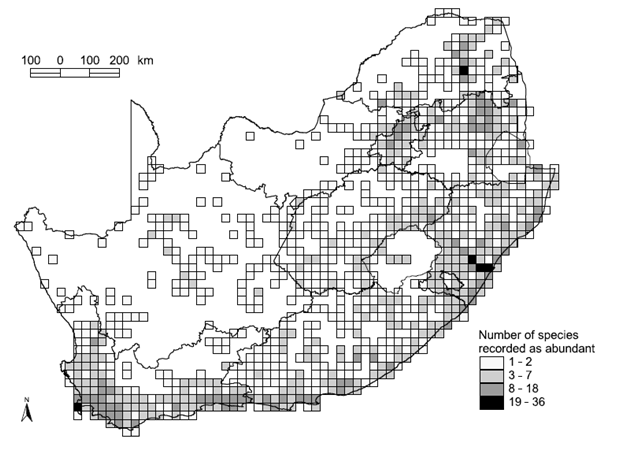
\includegraphics[scale = 0.8]{Images/SA_map}
	\caption{Distribution of alien invasive plants in South Africa (\cite{Henderson2001}).}
	\label{fig:SAmap}
\end{figure}

\clearpage
\noindent A 1996/7 survey conducted by \citet{Maitre2000} estimated that IAPs occupied approximately 10.1 million ha (or 1.736 million condensed ha) of South Africa. Combined estimates published 14 years later by \citet{Kotze2010} and \citet{VandenBerg2010} raised that figure to 1.813 million condensed ha. The annual economic cost associated with the damage inflicted by these IAPs was estimated to be approximately R6.5 billion (at 2008 inflation values) \citep{DeLange2010}. Water loss and the degradation of grazing land were the highest contributors to this figure.\newline 
One of the major groups of IAPs in both South Africa and Australia are the Cactaceae \citep{Moran1991BiologicalAfrica, Zimmermann2009, Klein2011,Paterson2011BiologicalAfrica}. The first successful biological control initiative on record for a weed was for the control of \textit{Opuntia monacantha} Haworth in India in the 1800s, and was the result of a misidentification of a \textit{Dactylopius} species \citep{Greenfield2005,Zimmermann2009}. \textit{Dactylopius ceylonicus} Green (Hemiptera: Dactylopiidae) was initially introduced to India in the belief that it was \textit{D. coccus}; a species reared for its high output of carminic acid used for the production of red dye. The insect caused such damage to \textit{O. monacantha} that the dye industry failed, but the insect continued to be used as a control agent for \textit{O. monacantha} infestations in the country, and in Sri Lanka \citep{Zimmermann2009}. Following its success in India, South Africa released \textit{D. ceylonicus} to combat \textit{O. monacantha} in 1913, which resulted in complete control of the weed within a few years and is the first intentional biological control programme on record globally \citep{lounsbury1915,Zimmermann2004BiologicalWater, Paterson2011BiologicalAfrica}. Australia followed suit and released \textit{D. ceylonicus} in 1914, which established successfully and delivered widespread control of the same weed \citep{Winston2014BiologicalWeeds.}. \\
The Dactylopiidae family (\textit{Dactylopius} Costa) is predominantly host specific to cactaceous species in the \textit{Opuntia} and \textit{Nopalea} genera \citep{DeLotto1974, Campana2015, VanDam2015}. These two cactus genera are genetically and taxonomically closely related \citep{griffith2009phylogeny}. The Dactylopiidae family is monogeneric and comprises eleven species of cactophagous insects (commonly referred to as `cochineal') \citep{Campana2015, VanDam2015}. Four \textit{Dactylopius} species are used in South Africa and Australia as biocontrol agents for invasive \textit{Opuntia} and \textit{Cylindropuntia} (Engelm.(Kuth)) cacti \citep{zachTable}. Twelve other countries around the world have released \textit{Dactylopius} species to control invasive cacti, where the impacts recorded are generally very high when establishment was successful \citep{Winston2014BiologicalWeeds.}. Many of the \textit{Dactylopius} species contain distinct genetic groups that display differential host specificities \citep{Volchansky1999, Mathenge2009,  Mathenge2010a, Mathenge2010, Jones2015, Mathenge2015}. These intraspecific groups are frequently referred to as `biotypes' in the literature, but in agreement with the criticism raised by \citet{Downie2010}, this thesis will instead use the term `lineage'. This is discussed in detail in Section \ref{sec:biotypes}. It is currently impossible to distinguish between \textit{Dactylopius} lineages using morphological characteristics \citep{Mathenge2015, jones2016host}, raising a need to address this using genetic methods. Being able to identify the species and lineages of \textit{Dactylopius} insects is fundamental to the practice of biological control of Cactaceae worldwide.  
\section{Impacts of Invasive Species}
 
Alien invasive organisms have the potential to significantly alter novel environments and affect native species at the genetic through to the ecosystem level \citep{Thompson1991, Crooks, Lockwood2013}.  \citet{Vila2017} grouped the impacts of invasive species on ecosystem services into four categories; namely that of 1) supporting, 2) provisioning, 3) regulating, and 4) cultural and human well-being. \\
Supporting services include important ecosystem processes incorporating nutrient and energy flows, such as carbon sequestration and primary production, nutrient cycling, habitat structure, and hydrology. As an example, invasive \textit{Acacia mearnsii} De Wild. (black wattle) dominate riparian zones in South Africa and use significantly more water than indigenous plants. This causes major reductions in water catchment yields and streamflow \citep{Maitre2000, Dye2004}. \citet{Maitre2000} estimated that IAPs in South Africa use approximately 3.3 billion m\textsuperscript{3} of water annually. This is a very disconcerting figure taking into account that many parts of the country face severe water shortages. \\
% \textit{Spartina alterniflora} Loisel. (`smooth cordgrass'), for example, is an invader of coastal wetlands and causes a significant increase in primary production, and hence the increased availability of soil organic carbon \citep{Nie2017}. Similarly, the nitrogen-fixer \textit{Morella faya} Aiton (`fire tree') increased the nitrogen content of soils in invaded areas of Hawaii by one order of magnitude \citep{Vitousek1989}. Among other effects, this large nutrient input facilitated the secondary growth of other invasive weeds such as \textit{Psidium cattleianum} Sabine (`strawberry guava'), and altered primary succession patterns on young volcanic rock sites \citep{Vitousek1989}. A similar effect was seen in South Africa, where invasive \textit{Acacia saligna} Labill. (Wendl.) facilitated the growth of a secondary grass invader (\textit{Ehrharta calycina} Smith) in the Fynbos region due to nitrogen fixation \citep{Yelenik2018a}. Many invasive species proceed to alter habitat structure, such as altering light and water availability \citep{Yelenik2018a, Asner2008}, rates of sedimentation \citep{Daehler1996,DiTomaso1998}, erosion \citep{VanWilgen1985} and water quality \citep{VanWilgen2011,DeLange2010,Chamier2012}. For example, \textit{Eichhornia crassipes} (Solms. Laubach), one of the world’s worst aquatic weeds, alters habitats by forming dense mats over freshwater bodies \citep{Cilliers1991}. This prevents sunlight from reaching native submerged plants, contributes to evapotranspiration and sedimentation and depletes dissolved oxygen in the surrounding water \citep{Cilliers1991, VanWyk2002, VanWilgen2011}. The weed is also known to block waterways, impede water flow and damage infrastructure \citep{Cilliers1991, Catford2012}. Invaders can disrupt and modify hydrological systems \citep{LeMaitre1996, Pejchar2009, Catford2012}, such as \textit{Tamarix} L. spp. (salt cedars) in the United States \citep{DiTomaso1998} and \textit{Pinus} L. \citep{Scott1997}, \textit{Eucalyptus} L’ Hér. \citep{Dye2013}, \textit{Prosopis} \citep{Maitre2000} and \textit{Acacia} Martius \citep{VanLill1980} spp. in South Africa. \citet{Zavaleta2000}, for example, estimated that \textit{Tamarix ramosissima} Ledeb. used 1.4-3.0 billion m\textsuperscript{3} more water than native plants in the south western United States. Similarly, \textit{Acacia mearnsii} De Wild. (black wattle) dominates riparian zones and uses significantly more water than indigenous plants, which can cause major reductions in water catchment yields and streamflow \citep{Maitre2000, Dye2004}. \citet{Maitre2000} estimated that IAPs in South Africa use approximately 3.3 billion m\textsuperscript{3} of water annually. \newline 
Provisioning services include the resources humans need for food, fuel, water, and other essential materials such as fibre \citep{Pejchar2009,Vila2017}. Approximately 10\% of the Earth's land surface comprises arable land used for agriculture and horticulture \citep{Fried2017}. These areas are particularly vulnerable to biological invasions due to the high incidence of fertilisation and disturbance, where weeds can interfere through competitive, allelopathic, and parasitic mechanisms \citep{Fried2017}. \textit{Parthenium hysterophorus} L. (‘famine weed’), for example, has invaded agricultural lands in parts of Africa, Asia, and Australia \citep{Mcconnachie2011}. The weed is highly competitive and allelopathic, and releases phenolics and sesquiterpenes into the surrounding soil that inhibits the growth of important crops such as cereals, vegetables, and grasses \citep{Evans1997}. \\
% \textit{Centaurea solstitialis} L. (yellow star thistle), for example, is a weed native to Europe that is unpalatable to grazing livestock, and causes major losses in forage yields in California \citep{Eagle2007}. Another highly damaging weed native to Central America, \textit{Parthenium hysterophorus} L. (‘famine weed’), has invaded agricultural lands in parts of Africa, Asia and Australia \citep{Mcconnachie2011}. The weed is highly competitive and allelopathic, releasing phenolics and sesquiterpenes into the surrounding soil that inhibits the growth of important crops such as cereals, vegetables and grasses \citep{Evans1997}. Some recorded crop losses are severe, such as an approximate 40-97\% loss in sorghum yield in Ethiopia \citep{Tamado2002InterferenceCompetition}, crop losses of up to 40\% in India \citep{Kohsla1981} and a reduction in the carrying capacity of some farms in Australia and India by approximately 40 and 90\%, respectively \citep{McFadyen1992, Evans1997}. Additionally, the weed can serve as a reservoir for crop pests \citep{Robertson}, degrade grazing areas \citep{McFadyen1992} and cause severe health implications for livestock (such as gastrointestinal irritation, dermatitis, anorexia and death) \citep{Evans1997}. Many invasive aquatic macrophytes cause large-scale damage to fisheries and nursery grounds, such as \textit{Lagarosiphon major} Ridl. (`curly water weed'), \textit{Myriophyllum aquaticum} Vell. Verd. (`parrot’s-feather'), \textit{Crassula helmsii} Kirk. Cockayne (`New Zealand pigmyweed'), \textit{Alternanthera philoxeroides} Griseb (`alligator weed'), \textit{Lythrum salicaria} L. (`purple loosestrife') and \textit{Caulerpa taxifolia} M. Wahl. (`killer alga') \citep{Gozlan2017}. These weeds tend to deplete dissolved oxygen, alter water chemical profiles, decrease light penetration, outcompete native plant life and ultimately modify community structures and trophic interactions \citep{Schultz2012, Gozlan2017}. 
Regulating services are those that sustain and adjust an ecosystem, such as pollination services, disturbance regimes, food webs, water purification, soil stabilization, climate regulation, and the role of endemic species (e.g. mutualistic relationships) \citep{Pejchar2009, Vila2017}. As an example of how a disturbance regime can be affected, invasive plants can alter fire regimes by serving as a fuel source and promoting more intense fires \citep{DAntonio1992, Brooks2004,Milton2004,LeMaitre2014}. This allows invaders to outcompete native species that are not suitably adapted to this disturbance and do not recover as quickly \citep{Milton2004}. \\
% Invasive plants can alter fire regimes by serving as a fuel source and promoting frequent fires \citep{DAntonio1992, Brooks2004,Milton2004,LeMaitre2014}. This allows invaders to outcompete native species that are not suitably adapted to this disturbance and do not recover as quickly \citep{Milton2004}. Invasive perennial grasses are particularly notorious \citep{DAntonio1992}, such as \textit{Arundo donax} L. (`Spanish reed'), \textit{Nassella tenuissima} Trin. Barkworth (`tussock grass') and \textit{Pennisetum setaceum} Forssk. Chiov. (‘crimson fountain grass’) \citep{Milton2004}. \citet{VanWilgen1985} conducted a fire simulation study using \textit{Hakea sericea} Schrad. (`silky hakea') and \textit{Acacia saligna} (Labill.) Wendl., (`Port Jackson willow') and found that these two shrubs increased fuel load by 60\% and 50\%, respectively. Fires also alter nutrient budgets in ecosystems by volatizing and converting elements such as nitrogen and carbon into more bioavailable forms \citep{DAntonio1992}. The impacts of invasive species on food webs are extensive (see a review by \citet{David2017a}). One classic example is that of the invasive \textit{Anoplolepsis gracilipes} Smith (Hymenoptera: Formicidae) (`yellow crazy ant') on Christmas Island \citep{ODowd2003}. \textit{Gecarcoidea natalis} Pocock (`red land crab') is endemic, and serves as a keystone species in ecosystem functioning in the forests on the island \citep{ODowd2003}. The crustacean regulates processes such as seedling recruitment, leaf litter degradation and the density of litter invertebrates \citep{Green1997, Green1999a}. \textit{Anoplolepsis gracilipes} form supercolonies, and attack and kill \textit{G. natalis} by spraying formic acid into their eyes and mouths \citep{ODowd2003}. The crabs are particularly vulnerable to attack during their annual migration through the forest to the ocean shore \citep{ODowd2003}. Declines in the population numbers of \textit{G. natalis} have been shown to have both bottom-up and top-down effects on the forest ecosystem that affect multiple trophic levels; namely through the change in vegetation composition and the association of scale insects with the invasive ant \citep{ODowd2003}. These sap-sucking scale insects cause die-back of the forest canopy cover \citep{ODowd2003}. \newline 
Cultural and human well-being services entail the aesthetics of nature and the spread of diseases \citep{Vila2017}. For example, \textit{Eichhornia crassipes} infestations in fresh water bodies limits boating activity and other water recreation activities \citep{Villamagna2018}. Invaded areas tend to display lower diversity, where invasive species tend to dominate the landscape and reduce its aesthetic value \citep{Kueffer2017}. Invasive species can act as vectors and reservoirs of diseases, such as \textit{Aedes aegypti} L. (`yellow fever mosquito') and \textit{A. albopictus} Skuse (`Asian tiger mosquito') (Diptera: Culicidae) that vector the Chikungunya virus, and \textit{Phlebotomus} Loew and \textit{Lutzomyia} França spp. (`sandflies') (Diptera: Psychodidae) that vector Leishmania pathogens \citep{Rabitsch2017}. \\
% Conflicts of interest arise when an invasive species holds economic value in its introduced range, such as \textit{Opuntia ficus-indica} L. (Mill.), which is both highly invasive and a source of income for many rural communities in South Africa \citep{Brutsch1993ThePlants, Beinart2011}. The prickly pear fruit is harvested and sold, and is also used to make beer, jam, and traditional medicines \citep{Brutsch1993ThePlants, shackleton2011invasive}. Rural communities in the Eastern Cape in particular rely heavily on the fruit for an income, and the local people are generally unaware of its invasive status   \citep{shackleton2007assessing}. Greater communication between these informal traders and the municipality is necessary, where legislation needs to be implemented that achieves a balance between limiting the negative effects of the invader on the environment, and promoting economic growth \citep{shackleton2011invasive}. \\
% Cultural services associated with the recreation and tourism industry are relatively easier to quantify, such as the cost associated with \textit{Myriophyllum spicatum} L. (`Eurasian water milfoil') on Lake Tahoe in the USA, and the decline in outdoor activities due to the lacerations caused by \textit{Centaurea solstitialis} L. (`yellow star thistle') and stings by \textit{Solenopsis invicta} Buren (`red imported fire ant') \citep{Pejchar2009}. Other invasive species, such as venomous spiders (e.g. \textit{Latrodectus hasselti} Thorell, `widow spiders' (Araneae: Theridiidae)), wasps (e.g. \textit{Vespula germanica} Fabricius, `German yellowjacket' (Hymenoptera: Vespidae)), fish (e.g. \textit{Pterois volitans} L., `lionfish' and \textit{Lagocephalus sceleratus} Gmelin, `pufferfish'), snakes (e.g. \textit{Boiga irregularis} Merrem, `brown tree snake') and plants (e.g. \textit{Solanum nigrum} L., `European black nightshade'), can be harmful to humans, sometimes even fatal \citep{Nentwig2017}. 
The impacts associated with invasive Cactaceae touch on all four invasion impact categories, predominantly relating to the loss of biodiversity, ecological functioning, and agricultural output \citep{kaplan2017proposed, novoa2019spinelessness}. Areas of dense cactus infestation leads to the exclusion of indigenous plants and animals through competitive exclusion and damage caused by spines and glochids \citep{walters2011}. Negative impacts on agricultural practices are caused by reduced grazing areas for livestock and the resulting decrease in productivity, costs incurred by mechanical and chemical control practices (where the costs of control sometimes exceed the value of the land itself), injuries to livestock caused by spines, and damage to fleece and hides \citep{Lloyd2014}. 
\section{Biological control}
\subsection{Overview}
\citet{VanDriesche2009} defines biological control as \textit{``The use of populations of natural enemies to suppress pest populations to lower densities, either permanently or temporarily''}. Biological control is a broad term encompassing the following methods: 
\vspace{0.4cm}
\begin{enumerate}
    \item `Classical', which is the most common approach, and refers to the use of natural enemies from the native range of a target pest (which share an evolutionary history) to achieve control.
    \item `Neo-classical' or `new association' methods, which makes use of non-native agents to control native species (which share no previous evolutionary history).
    \item `Augmentative', where the natural enemies of a target pest are mass-reared and released in order to augment naturally occurring enemy populations.
    \item `Conservation', which focuses on the maintenance of natural enemy populations in order to optimise their efficacy as parasitoids, pathogens, or predators. \\
    \citep{mcfadyen1998biological, collier2004critical,  VanDriesche2009, gullan2014insects, begg2017functional}.
\end{enumerate}
\vspace{0.4cm}

 \noindent Classical biological control is based primarily upon the enemy release hypothesis (ERH), which proposes that when a plant species is introduced into a new environment, it is released from its natural enemies (particularly specialist enemies) and is more readily able to spread quickly and invest resources into growth and reproduction \citep{keane2002exotic, mcevoy2002insect, liu2006testing}. This often involves energy trade-offs where chemical and structural defenses are down-regulated in favour of rapid growth and seed production \citep{blossey1995evolution, van1996optimal}. The ERH also predicts that it will be rare for the natural enemies of native plants to switch hosts and begin feeding on the invader, and that native generalist enemies will be more likely to feed on native species \citep{keane2002exotic}. \\
The benefits of biological control include: 
\vspace{0.4cm}
\begin{enumerate}
    \item Permanency of control and the self-perpetuation of agent populations.
    \item Host-specificity with little chance of non-target effects.
    \item High cost-to-benefit ratios relative to mechanical and chemical control methods.
    \item Being environmentally friendly (involving no toxic residues, and requiring a low energy input).
    \item Being able to naturally spread across the range of the host plant.
    \item The ability to be used in combination with other control methods as part of an integrated pest management (IPM) programme. \\
    \citep{hokannen1995, vanWilgen2004TheAfrica, culliney2005benefits, VanDriesche2009, zachariades2017assessing}.
\end{enumerate}

\subsection{The biological control pipeline}

A review by \citet{mcfadyen1998biological} summarised the steps involved in a biological control programme as follows: exploration in the weed's region/s of origin $\rightarrow$ selection of potential agents $\rightarrow$ host specificity testing $\rightarrow$ mass rearing of the chosen agent/s $\rightarrow$ releases into target areas $\rightarrow$ post-release evaluation and the implementation of integrated control strategies. The two central steps are that of agent selection and host specificity testing, which will briefly be reviewed here.

\subsubsection{Agent selection and prioritisation}

There is often an array of phytophagous species associated with a particular host plant \citep{frost1954numerical, southwood1961number}, but they do not all inflict the same mode and/or level of damage. \citet{wilson1960}, for example, reported that only five of the 52 insects imported for the control of \textit{Opuntia ficus-indica} in Australia could serve as damaging agents. The costs and time required for testing can quickly become unfeasible and impractical \citep{harris1991classical, mcfadyen1998biological, paterson2014prioritisation}. Host specificity testing is estimated to take approximately three scientist years and AUD\$460 000 (at 1997 prices) per agent \citep{mcfadyen1998biological}. The prioritisation of agents is thus integral to a biological control programme, such that only the most effective candidates are selected to deliver the highest level of targeted damage possible. This concept is central to this thesis, as the identification of the correct \textit{Dactylopius} lineage is necessary to inflict the most damage to the target cactus species.  Quoting \citet{mcfadyen1998biological}, predicting the success of an agent prior to release and selecting the most effective one is the `holy grail of weed biocontrol'. A number of factors need to be considered in order to select the most suitable candidate, including the following from a general scoring system originally proposed by \citet{harris1973selection} and modified by \citet{goeden1983}:
\vspace{0.4cm}
\begin{enumerate}
    \item The degree of host-specificity displayed (the agent must express suitable levels of specialisation for release in the introduced range).
    \item The level of direct and indirect damage caused to the host plant (where damage to vascular and mechanical support tissue is the most effective).
    \item Phenology of attack (where a prolonged attack is optimal that extends over the growing and/or reproductive phase of the target weed)
    \item The number of generations and progeny per generation produced (where a multivoltine and highly fecund agent is desired).
    \item Extrinsic mortality factors (where ideally only specialised natural enemies are associated with the agent, and competition by other species for the host plant is negligible).
    \item Feeding behaviour (where gregarious feeding is desired for greater damage).
    \item Compatibility with other agents.
    \item Distribution (where ideally the agent covers a large part of the range of the target weed).
    \item Previous successes as a biological control agent in other parts of the world.
\end{enumerate} 
\vspace{0.4cm}
Although the proposed scoring system was criticised for not being thorough enough \citep{wapshere1985effectiveness, cullen1995, kriticos2003}, it presented an initial framework and opened further discussion. \citet{cullen1995}, \citet{kriticos2003}, and \citet{klinken2006scientific} suggest that a more integrative approach to agent selection should be based on ecological modelling. This involves understanding the interactions between the agent and its host plant, and being able to predict how various factors such as disturbance regimes, competition, plant succession, different life stages of the host plant, and climatic variation may influence their dynamics \citep{mcevoy1999biological}. 
Closely linked to the concept of ecological modelling is that of climatic and genotypic matching; where the climatic compatibility between the native and introduced range is assessed, and the genetic variation (i.e. the number of haplotypes present) in both the host plant and agent is considered \citep{iline2004allozyme, dhileepan2006systematic, goolsby2006matching, robertson2008climate, Paterson2009UsingControl, VanDriesche2009, paterson2014prioritisation, fischbein2019modelling, jourdan2019sourcing, sutton2019searching}.
 Despite all the tools available, extrapolating results from a controlled environment to field conditions remains a major challenge (see for example \citet{buccellato2019post}). 

\subsubsection{Host specificity testing}

The safety of a biological control programme is of vital importance, and requires a thorough risk assessment of the potential non-target effects that could arise following the release of an agent into a target area \citep{mcevoy1996host, secord1996perils, mcfadyen1998biological, heard1999concepts, vanklinken1999host, schaffner2001host, heard2002host, VanDriesche2009}. This form of risk assessment is referred to as `host specificity testing', and aims to elucidate what the agent's host range breadth is, and its relative acceptability of different host plant species \citep{vanklinken1999host}.  \citet{vanklinken1999host} outline three central steps in the testing process, namely: 
\vspace{0.4cm}

\begin{enumerate}
    \item Identifying which stages in an agent's life history need to be host-specific
(larval instars might display differential feeding behaviours, and adults might damage non-target plants through feeding, oviposition, or the transferal of pathogens).
\item Estimating the fundamental host range, which is the range of host plants on which the agent is capable of completing its life cycle \citep{schaffner2001host}. This is tested through the use of the centrifugal-phylogenetic method proposed by \citet{wapshere1974strategy}. The method entails the testing of an array of plant species in the agent's host range; beginning with those most closely related to the target weed, working outwards to more distantly related species. Plants occurring in the same habitat, that share similar chemical and/or morphological traits, or serve as hosts to congeneric insects to that of the target weed are included in the testing procedure. Importantly, economically important crops and rare and endangered species in the same family as the target weed are prioritised. The testing procedure encompasses choice and no-choice tests \citep{schaffner2001host}, continuation, oogenesis, and open-field tests \citep{VanDriesche2009, Schaffner2018}.
\item Extrapolating to the field, which involves predicting what the realised host range will be under field conditions. The realised host range comprises the host plants that the agent can develop on under field conditions, and is initially predicted by taking surveys of related host plants occurring sympatrically with the target weed \citep{schaffner2001host}, followed by open field tests if possible \citep{balciunas1996comparison}.
\end{enumerate}
\vspace{0.4cm}
In cases where test results indicate that an agent will cause damage to one or more non-target species, a cost to benefit assessment is required to determine whether the relative value of the non-target species is higher than the damage caused by the target weed \citep{mcfadyen1998biological, VanDriesche2009}. Cost to benefit analyses have been used in the past to determine whether an agent should be released \citep{mcfadyen1990leaf, olckers1995interpreting, cristofaro1998biology, haye2006controlling} \\
Risk assessments are important to determine potential non-target effects associated with a released agent \citep{paynter2015relative, paynter2018making, hinz2019safe}. This is done by quantifying the performance of an agent on target and non-target plants, and calculating risk scores that can predict the probability of attack \citep{paynter2015relative}.

\subsubsection{Biological control track record}

Using the data compiled by \citet{Winston2014BiologicalWeeds.}, \citet{schwarzlander2018biological} summarised that up to the year 2012, 468 biological control agent species have been released onto 175 weed species (comprising 48 plant families) across the world. Of the agents released, 70.9\% established successfully. Post-release surveys determined that only 7\% of releases resulted in no impact at all on the target weed, and that 55\% of agents caused heavy, medium, or variable impact in at least one release. Of the targeted 175 weed species, 115 (65.7\%) have been controlled to some degree by at least one biological control agent. \\  
A review by \citet{hinz2019safe} stated that of the 457 species of biological control agents intentionally released between the years 1863 and 2008, 60 (13.1\%) were associated with non-target attacks (NTAs). Of those 60 NTAs, 42 involved attacks on native species. In agreement with \citet{sheppard2003global} and \citet{suckling2014magnitude}, the review concluded that less than 1\% of all weed biological control releases have the potential to result in negative non-target effects. Additionally, it found that the proportion of agent releases associated with NTAs has decreased despite the increase in releases over the years. This is most likely due to a combination of more stringent host specificity testing measures and stricter regulations regarding the release of biocontrol agents. \citet{hinz2019safe} emphasise that post-release monitoring should be as important as pre-release host specificity testing in order to accurately quantify agent impact and NTAs.
\section{The Cactaceae}

There are approximately 130 genera and 2000 species in the Cactaceae family (order Caryophyllales); all of which are indigenous to the Americas \citep{Anderson2001, Wallace2002, Zimmermann2009, Novoa2015IntroducedReview, christenhusz2016number}. The one exception is the epiphyte \textit{Rhipsalis baccifera} Stern (`mistletoe cactus'), which is possibly native to southern Africa and Madagascar \citep{Wallace2002, Zimmermann2009}. The centre of cactus diversity in the native range is in Mexico, where the three most speciose genera are \textit{Opuntia}, \textit{Echinopsis}, and \textit{Mammillaria} \citep{Novoa2015IntroducedReview}. The Cactaceae family evolved about 65 mya in South America \citep{Anderson2001}, and radiated about 30 to 35 mya in response to the aridification of the Americas and increased atmospheric CO\textsubscript{2} \citep{Arakaki2011, Majure2012}. The Cactaceae comprise four subfamilies; namely the Pereskioideae, Cactoideae, Maihuenioideae, and Opuntioideae \citep{Labra2003}. Their distribution spans from southern Patagonia in Argentina to British Columbia in Canada \citep{Anderson2001, Edwards2005}. Most cactaceous plants are succulents and are adapted to extreme xeric environments, although some epiphytes have even been found to thrive in rain forests \citep{Anderson2001}. Most species possess leafless photosynthetic stems and protective spines, which are modified leaves arising from areoles \citep{eggli1993glossary}. The spines of cactaceous plants are adapted for a number of functions across different species, such as protection from herbivores, camouflage, thermoregulation, water conservation, and dispersal \citep{Anderson2001}.
The Cactaceae display a diverse range of growth forms and sizes, from the smallest species (\textit{Blossfeldia liliputana} Werdermann) measuring 9 mm in diameter to one of the largest that stands nearly 20 m tall (\textit{Pachycereus pringlei} Britton \& Rose, the `Giant Mexican cardon') \citep{Anderson2001}. Some botanists have classified 13 different growth forms within this family, ranging from globular and columnar, to leaf-like and clustering \citep{Anderson2001}. Cactaceous plants typically display a diploid chromosome system of 2n = 22, but numerous species in the Opuntioideae family are known to display polyploidy \citep{Anderson2001}. Additionally, asexual reproduction is common in many Cactaceae, where stem joints can break off the main plant, grow adventitious roots, and give rise to new plants \citep{Anderson2001}. \\
Although the Cactaceae are endemic to the New World, they have become naturalised widely outside their native distribution, and, in many cases, have become serious invaders \citep{Novoa2015IntroducedReview}. Of the 1922 cactus species reviewed by \citet{Novoa2015IntroducedReview}, 57 (3\%) were invasive in other parts of the world (Fig. \ref{fig:novoaMap}). The review reported that \textit{O. ficus-indica} was the most widespread invader; having been recorded in 22 countries outside its native range. The countries most heavily invaded by cactaceous weeds are Australia, South Africa, and Spain; with 39, 35, and 24 recorded species, respectively.
\vspace{0.4cm}

\begin{figure}[H]
	\centering
	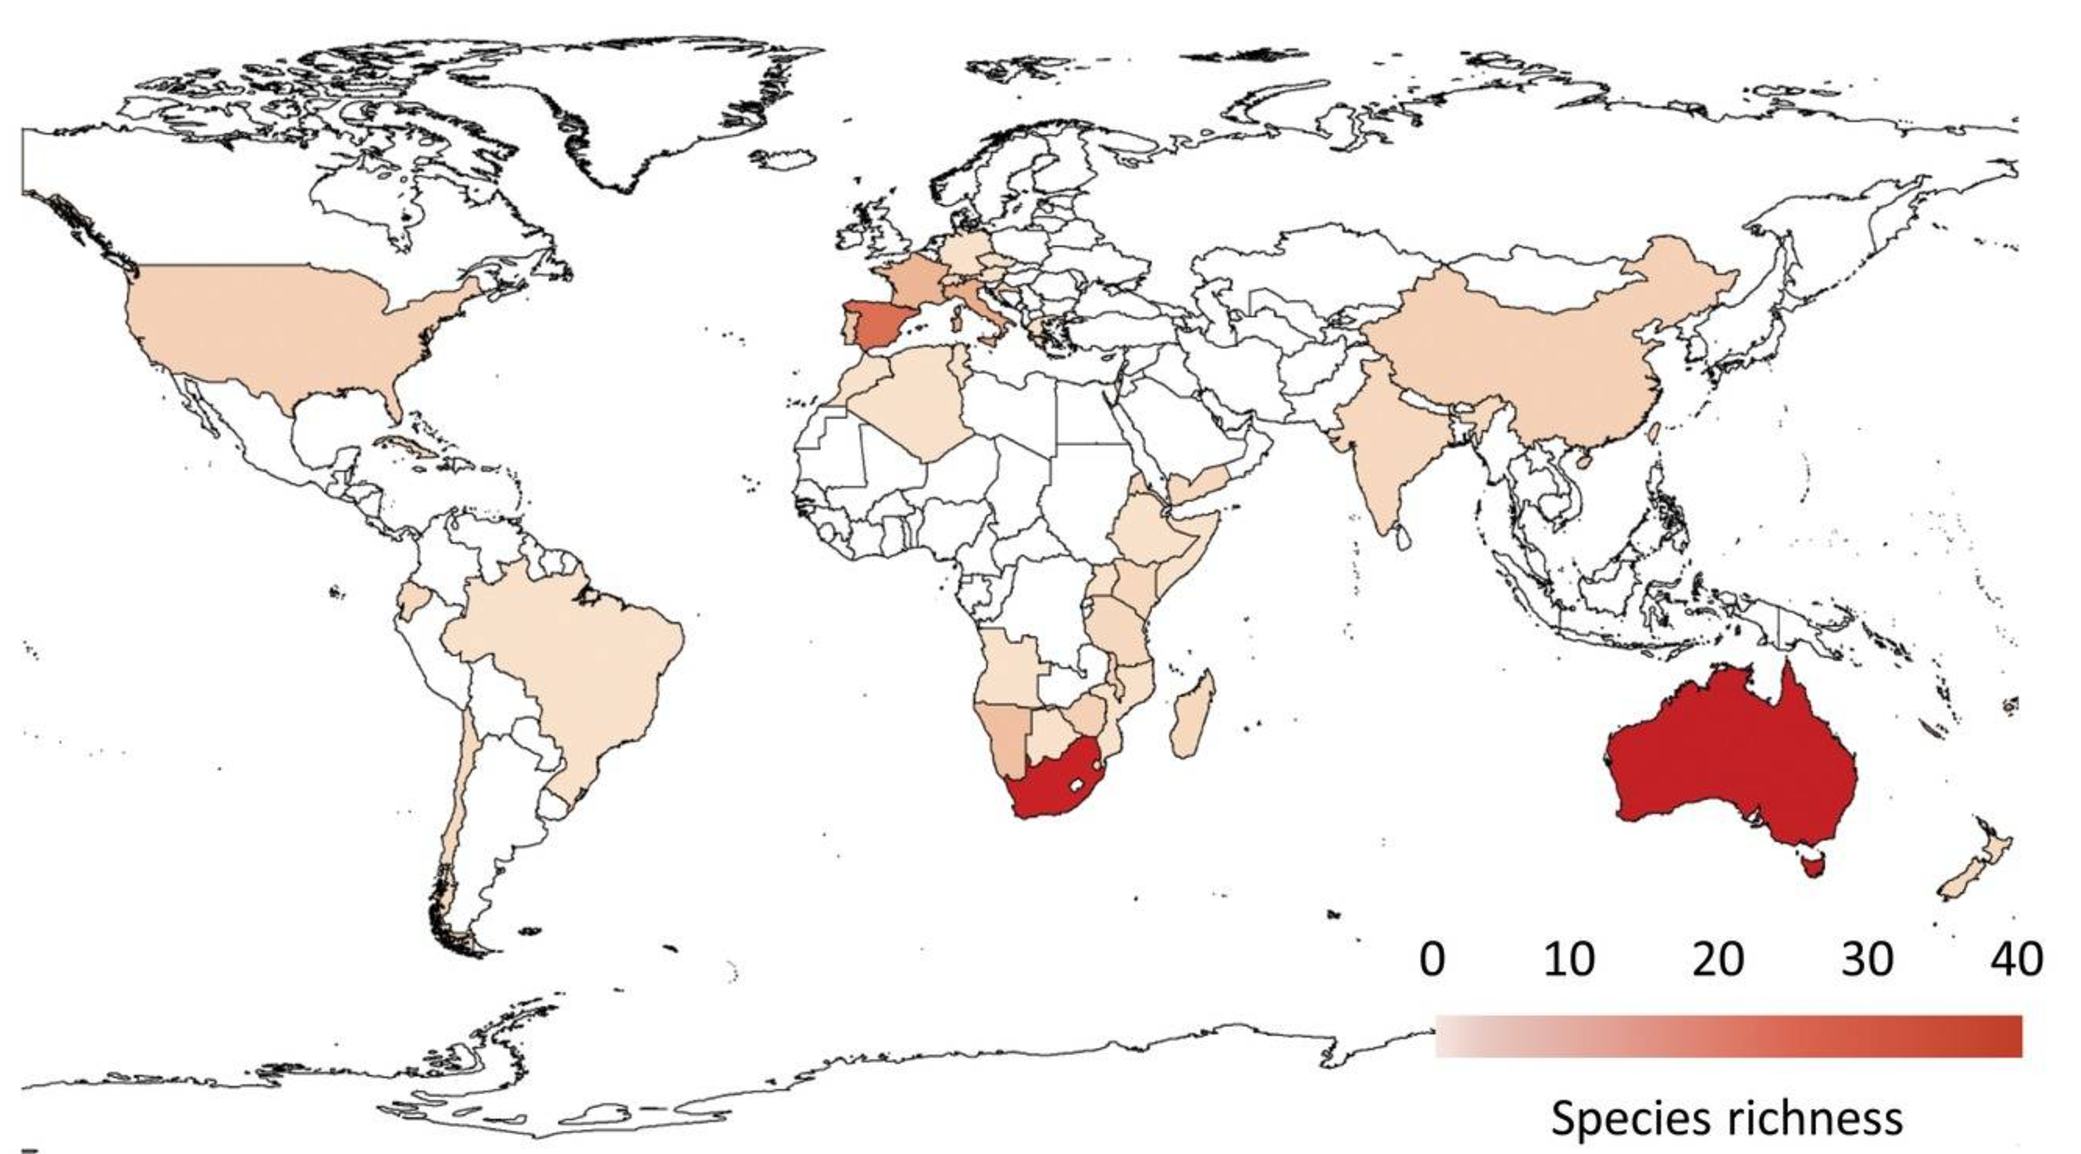
\includegraphics[scale = 0.45]{Images/novoa_map.pdf}
	\caption{The invasive range of 57 cactus species, as reviewed by \citet{Novoa2015IntroducedReview}.}
	\label{fig:novoaMap}
\end{figure}

\subsection{Biological control of invasive Cactaceae}

The two predominant countries implementing cactus biocontrol are South Africa and Australia \citep{Moran1991a, paterson2019prospects}.
Numerous cactus species were introduced to these countries as ornamental and hedge plants, as a source of fruit and fodder, and for the establishment of a red dye industry during their early colonial periods \citep{Zimmermann2009, Paterson2011BiologicalAfrica, kaplan2017proposed, managingOpuntioid2017} (Tables \ref{tab:invasiveCactiSA} and \ref{tab:invasiveCactiAus}). There are four main groups of invasive cacti: namely the `platyopuntia' (e.g. \textit{Opuntia ficus-indica, O. stricta}, and \textit{O. monacantha}), `cylindropuntia' (e.g. \textit{Cylindropuntia imbricata}), `organ-pipe' (e.g. \textit{Harrisia martinii} and \textit{Cereus jamacaru}), and `leafy' (e.g. \textit{Pereskia aculeata}) \citep{Klein2002WeedsBiocontrol}. The main adaptations enabling the invasibility of these plants are their:
\vspace{0.4cm}
\begin{enumerate}
    \item Tolerance to xeric conditions and their water-efficient CAM (Crassulacean Acid Metabolism) photosynthetic strategy.
    \item Ability to outcompete native vegetation under disturbed conditions.
    \item Ability to reproduce both sexually and asexually. \\ \citep{Zimmermann2009}.
\end{enumerate}
\vspace{0.4cm}

\noindent Approximately 400 cactus taxa have been introduced to South Africa \citep{kaplan2017proposed}, of which 35 species are invasive \citep{Novoa2015IntroducedReview}. Twenty three of these have been subject to biological control using 19 insect species \citep{Zimmermann2009, Klein2011,Paterson2011BiologicalAfrica}. Of these, four are under complete control (\textit{Cereus jamacaru} D. C., \textit{Cylindropuntia fulgida} Engelmann, \textit{C. leptocaulis} Knuth, and \textit{Harrisia martinii} Labour) and eight are under substantial control (\textit{Cylindropuntia imbricata} Haworth, \textit{Harrisia balansae} (K.Schum.)  N. P. Taylor \& Zappi, \textit{Opuntia aurantiaca} Lindley, \textit{O. engelmannii} Salm-Dyck ex. Engelm., \textit{O. ficus-indica} (L.) Mill., \textit{O. monacantha} Haworth. \textit{O. salmiana} J. Parm. ex Pfeiff, and \textit{O. stricta}  Haworth) \citep{Klein2011}. \\
From 1920 to 1935, the Australian government funded the importation of 52 different potential cactus biocontrol agents for host specificity testing; of which 12 were released \citep{raghu2007understanding}. These included multiple \textit{Dactylopius} species, two \textit{Chelinidea} spp. (Hemiptera: Coreidae), an \textit{Olycella} sp. (Lepidoptera: Pyralidae), and \textit{Tetranychus opuntiae} (Acari: Tetranychidae) \citep{raghu2007understanding}. Additionally, \textit{Cactoblastis cactorum} (Lepidoptera: Pyralidae) was released in 1925 and established successfully \citep{mann1970cacti}; destroying hundreds of hectares of \textit{Opuntia}-infested areas within two years \citep{raghu2007understanding}.
Australia currently has 39 recorded invasive cactus taxa belonging to four genera; and is the most heavily invaded of all the countries surveyed by \citet{Novoa2015IntroducedReview}. Twenty-seven species are listed in the Weeds of National Significance (WoNS) database (Table \ref{tab:invasiveCactiAus}) \citep{managingOpuntioid2017}. Of the naturalised species, \textit{Corynopuntia} sp., \textit{O. dejecta}, and \textit{O. ficus-indica} are not considered invasive \citep{managingOpuntioid2017}. The two most prominent biological control agents in use are \textit{C. cactorum} and four \textit{Dactylopius} species; namely \textit{D. austrinus}, \textit{D. ceylonicus}, \textit{D. opuntiae}, and four \textit{D. tomentosus} lineages \citep{managingOpuntioid2017}. \\
The absence of indigenous Cactaceae and its relatives outside the New World allows for the use of less host-specific (oligophagous) agents in invaded areas, as there is a lower risk of non-target attack \citep{Zimmermann2002}. This also means that multiple target weeds can be attacked by oligophagous agents \citep{paterson2019prospects}. \\

\begin{table}[H]
\caption{National Environmental Management: Biodiversity Act (NEM:BA) Category 1 and 2 invasive cactus species in South Africa. Category 1a and 1b weeds require compulsory control, and need to be removed and destroyed. Category 2 weeds are regulated by area, and require demarcation permits (none are, however, allowed in riparian zones) \citep{nemba}.} \label{tab:invasiveCactiSA} 
\renewcommand{\arraystretch}{0.5}
\resizebox{\columnwidth}{!}{%
\begin{tabular}{@{}lll@{}}
\toprule
\textbf{Species} & \textbf{Common name} & \textbf{Category} \\ \midrule
\textit{Austrocylindropuntia cylindrica} (Juss. ex Lam.) Backeberg. & Cane cactus & 1a \\
\textit{Austrocylindropuntia subulata}
(Muehlenpf.) \\ Backeb. subsp. exaltata 
(A. Berger) D. R. Hunt & Long spine cactus & 1b \\
\textit{Cereus hexagonus} (L.) Mill. & Queen of the night & 1b \\
\textit{Cereus hildmannianus} K. Schum. & Queen of the night & 1b \\
\textit{Cerues jamacaru} D. C. & Queen of the night & 1b \\
\begin{tabular}[c]{@{}l@{}}\textit{Cylindropuntia fulgida} (Engelm.)\\ F. M. Knuth var. \textit{fulgida} \end{tabular} & Chain-fruit cholla & 1b \\
\begin{tabular}[c]{@{}l@{}}\textit{Cylindropuntia fulgida} (Engelm.)\\ F. M. Knuth var. \textit{mamillata} (Schott ex\\ Engelm.)\end{tabular} & Boxing glove cactus & 1b \\
\begin{tabular}[c]{@{}l@{}}\textit{Cylindropuntia imbricata} (Haw.)\\ F. M. Knuth\end{tabular} & Imbricate cactus & 1b \\
\textit{Cylindropuntia leptocaulis} (D. C.) F. M. Knuth & Pencil cactus & 1b \\
\textit{Cylindropuntia pallida} (Rose) F. M. Knuth & Pink-flowered sheathed cholla & 1a \\
\textit{Cylindropuntia spinosior} (Englem.) F. M. Knuth & Cane cholla & 1a \\ 
\textit{Harrisia balansae} (K. Schum.) N. P. Taylor \& Zappi & Strangler prickly apple & 1a \\ 
\textit{Harrisia martinii} (Labour.) Britton & Moon cactus & 1b \\
\textit{Harrisia pomanensis} (F. A. C. Weber) Britton \& Rose & Midnight lady & 1a \\
\textit{Harrisia tortuosa} (J. Forbes ex Otto \& A. Dietr.) \\ Britton \& Rose & Spiny snake cactus & 1b \\
\textit{Hylocereus undatus} (Haw.) Britton \& Rose & Night-blooming cereus & 2 \\
\textit{Myrtillocactus geometrizans} (Mart.) Console & Bilberry cactus & 1a \\
\textit{Opuntia aurantiaca} Lindl. & Jointed cactus & 1b \\
\textit{Opuntia elata} Link \& Otto ex Salm-Dyck & Orange tuna & 1b \\
\textit{Opuntia engelmannii} Salm-Dyck ex Engelm. & Small round-leaved prickly pear & 1b \\
\textit{Opuntia ficus-indica} (L.) Mill. & Sweet prickly pear & 1b \\
\textit{Opuntia humifusa} (Raf.) Raf & Creeping prickly pear & 1b \\
\textit{Opuntia leucotricha} D. C. & Aaron's-beard prickly pear & 1b \\
\textit{Opuntia microdasys} (Lehm.) Pfeiff & Yellow bunny-ears & 1b \\
\textit{Opuntia monacantha} Haw & Drooping prickly pear & 1b \\
\textit{Opuntia pubescens} J. C. Wendl. ex Pfeiff. & Velvet bur cactus & 1a \\
\textit{Opuntia robusta} H. L. Wendl. ex Pfeiff & Blue-leaf cactus & 1a \\
\textit{Opuntia salmiana} J. Parm. ex Pfeiff & Bur cactus & 1a \\
\textit{Opuntia spinulifera} Salm-Dyck & Saucepan cactus & 1b \\
\textit{Opuntia stricta} (Haw.) Haw. var. \textit{stricta} \\
and var. \textit{dillenii} (Ker Gawl.) L. D. Benson  & Pest pear of Australia & 1b \\
\textit{Opuntia tomentosa} Salm-Dyck & Velvet opuntia & 1b \\
\textit{Peniocereus serpentinus} (Lag. \& Rodr.) N. P. Taylor & Serpent cactus & 1b \\
\textit{Pereskia aculeata} Mill. & Barbados gooseberry & 1b \\
\textit{Tephrocactus articulatus} (Pfeiff.) Backeb. & Pine cone cactus & 1a \\
\bottomrule
\end{tabular}
}
\end{table}

\clearpage

\begin{table}[H]
\caption{List of the Cactaceae in the Australian Weeds of National Significance (WoNS) database \citep{managingOpuntioid2017}.} \label{tab:invasiveCactiAus} 
\renewcommand{\arraystretch}{0.5}
\centering
\begin{tabular}{@{}ll@{}}
\toprule
\textbf{Species} & \textbf{Common name} \\ \midrule
\textit{Austrocylindropuntia cylindrica} & Cane cactus \\
\textit{Austrocylindropuntia subulata} & Eve’s needle cactus \\
\textit{Cylindropuntia fulgida var. mamillata} & Coral cactus \\
\textit{Cylindropuntia imbricata} & Devil’s rope \\
\textit{Cylindropuntia kleiniae} & Klein's cholla \\
\textit{Cylindropuntia leptocaulis} & Pencil cactus \\
\textit{Cylindropuntia pallida} & White-spined Hudson pear \\
\textit{Cylindropuntia prolifera} & Jumping cholla \\
\textit{Cylindropuntia spinosior} & Snake cactus \\
\textit{Cylindropuntia tunicata} & Brown-spined Hudson pear \\
\textit{Opuntia aurantiaca} & Tiger pear \\
\textit{Opuntia elata} & Riverina pear \\
\textit{Opuntia elatior} & Red-flower prickly pear \\
\textit{Opuntia engelmannii} & Engelmann's prickly pear \\
\textit{Opuntia humifusa} &  \\
\textit{Opuntia leucotricha} &  \\
\textit{Opuntia microdasys} & Bunny ears \\
\textit{Opuntia sp. aff. microdasys} &  \\
\textit{Opuntia monacantha} & Drooping tree pear \\
\textit{Opuntia aff. polyacantha} &  \\
\textit{Opuntia puberula} &  \\
\textit{Opuntia robusta} &  \\
\textit{Opuntia schickendantzii} &  \\
\textit{Opuntia streptacantha} & Westwood pear \\
\textit{Opuntia stricta} var. \textit{stricta} and var. \textit{dillenii} &  \\
\textit{Opuntia sulphurea} &  \\
\textit{Opuntia tomentosa} & Velvet tree pear \\ \bottomrule
\end{tabular}
\end{table}

\subsubsection{\textit{Opuntia} Mill}

The \textit{Opuntia} genus is the most widespread of all the cacti, comprising approximately 180 species and numerous hybrids \citep{Anderson2001, Griffith2003}. \textit{Opuntia ficus-indica} L. (`sweet prickly pear') was likely one of the first cactus species introduced to South Africa in the early 1700s, and became widespread throughout the Karoo and Eastern Cape by the 1800s \citep{Annecke1978, Dean2000}. 
Numerous spineless varieties were bred in the early 1900s by the horticulturist Luther Burbank, and exported around the world as a source of food and fodder for livestock, and for its fruit \citep{anderson2015vast}. The first record of an \textit{Opuntia} species in Australia was in 1788, when the British brought both \textit{O. monacantha} and \textit{Dactylopius} species into the country to establish a red dye industry \citep{mann1970cacti}.
Many more \textit{Opuntia} species were introduced over the next few decades, and proceeded to cause major environmental damage and economic losses to the agricultural sectors in South Africa and Australia due to the growth of dense, impenetrable thickets on farmlands \citep{Dean2000}. \citet{novoa2019spinelessness} showed that spineless varieties grown from seeds (i.e. sexual reproduction) reverted back to their spiny form, which explains their high incidence in invaded regions. 
Mechanical and chemical control methods were initially implemented to control the weed, particularly the use of arsenical herbicides such as injectable monosodium methanearsonate (MSMA) \citep{Annecke1978,Zimmermann1991BiologicalAfrica}. \\ \textit{Opuntia stricta} Haworth (var. \textit{stricta}) (`Australian pest pear') was first recorded in Australia in 1839, and spread at a rate of 320 000 ha per year (at densities of about 250 000 kg per ha!) by the 1920s \citep{raghu2007understanding}. \textit{Dactylopius ceylonicus} was initially released to combat the weed in 1903, but did not establish because this insect is host-specific to \textit{O. monacantha}. The later release of the \textit{D. opuntiae} `stricta' lineage in 1921 caused substantial damage \citep{Winston2014BiologicalWeeds.}.
Following the success of the biological control of \textit{Opuntia stricta} Haworth (both subspecies, nameley var. \textit{stricta} and var. \textit{dillenii}) and \textit{O. ficus-indica} L. in Australia, four insects were successfully released in South Africa as an additional means to control the weed \citep{Annecke1978,Zimmermann1991BiologicalAfrica}. These were the cladode boring moth \textit{C. cactorum} Berg (Lepidoptera: Pyralidae) released in 1933, the cladode sucking cochineal bug \textit{D. opuntiae} (`ficus' lineage) Cockerell (Hemiptera: Dactylopiidae) released in 1938, and the stem boring beetles \textit{Lagocheirus funestus} Thompson (Coleoptera: Cerambycidae) released in 1943 and \textit{Metamasius spinolae} Gyllenhal (Coleoptera: Curculionidae) released in 1948 \citep{Klein2011}. Of these, \textit{C. cactorum}, and particularly \textit{D. opuntiae}, have been the most effective agents - to the point that the agents themselves were seen as a threat to commercial \textit{O. ficus-indica} plantations \citep{Zimmermann1991BiologicalAfrica}. This is currently the case in Brazil, Israel, and the Mediterranean area, where \textit{D. opuntiae} is threatening and/or causing substantial losses to the cactus fodder and fruit industry \citep{spodek2014first, torres2018management, mazzeo2019dactylopius}. Conflicts of interest are common in the control of invasive Cactaceae \citep{novoa2016resolving}, and arise when an invasive species holds economic value in its introduced range. 
For example, \textit{Opuntia ficus-indica} L. (Mill.) provides a source of income for many rural communities in South Africa \citep{Brutsch1993ThePlants, Beinart2011}. The fruit is harvested and sold, and is also used to make beer, jam, and traditional medicines \citep{Brutsch1993ThePlants, shackleton2011invasive}. Rural communities in the Eastern Cape Province in particular rely heavily on the fruit for an income, and the local people are generally unaware of its invasive status  \citep{shackleton2007assessing}. Greater communication between these informal traders and the municipality is necessary, where legislation needs to be implemented that achieves a balance between limiting the negative effects of the invader on the environment, and promoting economic growth \citep{shackleton2011invasive}. \\ 
\textit{Opuntia stricta} became particularly problematic in the Kruger National Park in South Africa; where elephants, baboons, and rivers aid in its dispersal \citep{hoffmann1998long}. \textit{Cactoblastis cactorum} was released in the park in 1988 to control the weed  \citep{Hoffmann1998EvaluationAfrica}, followed by \textit{D. opuntiae} (`stricta' lineage) in 1997 \citep{Klein2011}. Both these insects established successfully, where a biomass reduction of over 90\%, and an almost complete end to fruit production, has been recorded \citep{Paterson2011BiologicalAfrica}. The weed is currently considered to be under substantial control \citep{Klein2011}. \\
\textit{Opuntia aurantiaca} Lindley, commonly referred to as `jointed cactus', is indigenous to Argentina and Uruguay, and is thought to be a hybrid of \textit{O. discolor} Britton \& Rose and \textit{O. salmiana} J. Parm ex. Pfeiff \citep{Moran1991BiologicalAfrica}. 
% The botanist John Lindley first described \textit{O. aurantiaca} in 1833, and incorrectly claimed that it was native to Chile based on a misinterpreation of a report by the avid British plant collector John Gillies \citep{moran1976}. The name `\textit{aurantiaca}' stems from the Latin word `auros', meaning `gold'. The name was based upon a manuscript by John Gillies in which he recorded a cactus plant with orange flowers occurring in Chile and Mendoza, Argentina. Subsequent confusion arose regarding the identity of the plant, as the flowers originally described by Lindley were bright yellow. The cacti with orange flowers turned out to be a misidentification, and were in fact \textit{O. longispina} var. \textit{corrugata} Backeberg \citep{moran1976}.  
It is now accepted that \textit{O. aurantiaca} is native to east Argentina and Uruguay \citep{DeLotto1974, gunn1979, zimmermann1981JointedCactus}.
The weed was introduced to South Africa as an ornamental plant in 1843 from collections in the United Kingdom \citep{zimmermann1981JointedCactus}, and later became problematic in grazing areas in the Karoo region and the Eastern Cape Province \citep{Moran1991BiologicalAfrica}.
The first biocontrol agent to be released on this weed in Australia and South Africa was \textit{D. austrinus} De Lotto (Hemiptera: Dactylopiidae) in 1933 and 1935, respectively \citep{Moran1991BiologicalAfrica, Winston2014BiologicalWeeds.}. Only \textit{D. austrinus} and \textit{C. cactorum} established successfully on the weed \citep{Klein2011}, while the other three attempted agents failed (\textit{Mimorista pulchellalis} Dyar (Lepidoptera: Crambidae), \textit{Nanaia} spp. (Lepidoptera: Pyralidae), and \textit{Zophodia tapiacola} Dyar (Lepidoptera: Pyralidae)). 

\subsubsection{\textit{Cylindropuntia} (Engelmann) (Knuth)}
The \textit{Cylindropuntia} genus (commonly known as `chollas') is a monophyletic clade that falls within the Opuntioideae subfamily \citep{Anderson2001}. It was originally classified as a subgenus of \textit{Opuntia} in 1856, but was later placed in its own genus in 1935 \citep{Anderson2001}. The genus comprises 33 species, and, as with many of the \textit{Opuntia} species, undergoes natural hybridisation \citep{Anderson2001}. 
\textit{Cylindropuntia imbricata} was first introduced to South Africa in the early 1900s \citep{Moran1991BiologicalAfrica}. 
The weed was successfully controlled in Australia by \textit{D. tomentosus} after its release in the country in 1925 \citep{Dodd1940}. South Africa followed suit and released the insect in 1970 \citep{Moran1991BiologicalAfrica}. The only other biocontrol agent associated with the weed, \textit{Metamasius spinolae}, did not establish successfully \citep{Klein2011}. \\
\textit{Cylindropuntia fulgida} (Engelm. Knuth) (‘chain fruit cholla’) is a tree-like cactus that comes in two varieties; namely var. \textit{fulgida} and var. \textit{mamillata} \citep{Anderson2001}. \textit{Cylindropuntia fulgida} var. \textit{fulgida} was introduced to South Africa in the 1940s as an ornamental plant \citep{DeBeer1986}, and has become particularly damaging to pastoral lands in the Northern Cape and Limpopo Provinces \citep{Moran1991BiologicalAfrica,Paterson2011BiologicalAfrica}. The cactus was initially misidentified as \textit{C. rosea}, and as a result, biocontrol efforts were largely unsuccessful due to a less effective \textit{D. tomentosus} lineage being released \citep{Paterson2011BiologicalAfrica}. Following the correct identification of the weed, various \textit{D. tomentosus} lineages were collected in Mexico; namely from the two \textit{C. fulgida} varieties and from \textit{C. cholla} (F.A.C. Weber) (Knuth) \citep{Paterson2011BiologicalAfrica}. It was found that the \textit{C. cholla} lineage was the most damaging, and hence became the agent of choice for this cactus variety \citep{Mathenge2009a}. Other category 1a and 1b species in this genus in South Africa are \textit{C. pallida}, \textit{C. spinosior}, and \textit{C. leptocaulis} (Table \ref{tab:invasiveCactiSA}). In addition to these, Australia has listed \textit{C. kleiniae}, \textit{C. prolifera}, and \textit{C. tunicata} in their WoNS database (Table \ref{tab:invasiveCactiAus}).
\section{The Dactylopiidae}
The Dactylopiidae family (Hemiptera: Sternorrhyncha: Coccoidea) comprises 11 species and a variety of intraspecific lineages in the \textit{Dactylopius} genus; which are all indigenous to the Americas \citep{Rodriguez2001, VanDam2012} (Table \ref{tab:dactylopius_species}). 

\vspace{0.5cm}

\begin{table}[H]
\caption{A list of the 11 recorded \textit{Dactylopius} species and intraspecific lineages} \label{tab:dactylopius_species}
\centering
\renewcommand{\arraystretch}{0.5}
\begin{tabular}{@{}l@{}}
\toprule
\multicolumn{1}{c}{Species} \\ \midrule
\textit{Dactylopius austrinus} De Lotto \\
\textit{Dactylopius bassi} Targioni Tozzetti \\
\textit{Dactylopius ceylonicus} Green \\
\textit{Dactylopius coccus} Costa \\
\textit{Dactylopius confertus} De Lotto \\
\textit{Dactylopius confusus} Cockerell \\
\textit{Dactylopius gracilipilus} Van Dam \& May \\
\begin{tabular}[c]{@{}l@{}}\textit{Dactylopius opuntiae} Cockerell\\ Lineages: `ficus', and `stricta' \end{tabular} \\
\begin{tabular}[c]{@{}l@{}}\textit{Dactylopius tomentosus} Lamarck\\ Lineages: `bigelovii', `californica var. parkeri', \\ `cholla', `cylindropuntia sp.', `echinocarpa x \\ acanthocarpa', `imbricata' \end{tabular} \\
\textit{Dactylopius salmianus} De Lotto \\
\textit{Dactylopius zimmermannii} De Lotto \\ \bottomrule
\end{tabular}
\end{table}

\noindent  Four of these are currently used as biological control agents in South Africa and Australia; namely \textit{D. austrinus} De Lotto, \textit{D. ceylonicus} Green, \textit{D. opuntiae} Cockerell, and \textit{D. tomentosus} Lamarck \citep{DeLotto1974, Perez-Guerra1992, managingOpuntioid2017}. 
% These sap-sucking insects feed predominantly on cactaceous plants in the \textit{Opuntia} and \textit{Nopalea} genera \citep{DeLotto1974, VanDam2012, Campana2015}. 
All species produce carminic acid, a deep red anthraquinone, as a defensive compound \citep{Eisner1980, Perez-Guerra1992}. The Aztecs and Incas domesticated \textit{D. coccus} as a dye for wool, cotton, paint, and cosmetics \citep{Nobel2002CactiUses}. The dye has been used for over two thousand years, with the first historical reports from Peru dating back to the early 1500s \citep{Nobel2002CactiUses}. The Spanish conquistadors initiated large-scale cultivation of the insects in Oaxaca, Mexico, and began exporting them to Europe by the year 1526 \citep{Meyer2000}. The dye became the third highest source of income to the Spanish Empire after gold and silver \citep{Humboldt1966,Chavez-Moreno2009TheDistribution}.

\subsection{Identification issues}
The taxonomy of the Dactylopiidae is largely understudied, and until fairly recently, only morphological characters were used to create phylogenies \citep{Ramirez-Puebla2010MolecularBacteria}. The history of this insect's taxonomy is rooted in misidentifications. Many of the species are notoriously difficult to differentiate using morphological traits, even for experts \citep{Mann1969Cactus-feedingMites, Perez-Guerra1992, Gullan1997, Portillo2006AENEMIES}. Considering the high species diversity of the Cactaceae, the probability of there being many more \textit{Dactylopius} species, cryptic species, and lineages in the native range is very high. Using molecular tools to assist in the taxonomic organisation of this group is therefore very valuable. Different \textit{Dactylopius} species and lineages display different levels of damage on target Cactaceae, and so correctly distinguishing between them is fundamental to selecting the most effective agents for biological control programmes. This is where the use of genetic barcoding can be useful. 

\subsection{`Biotypes'}
\label{sec:biotypes}

Species within the Dactylopiidae consist of genetically and/or behaviourally-distinct groups, which have been referred to as `biotypes' in the literature \citep{githure1999host, Volchansky1999, Hoffmann2004a, Mathenge2009, Mathenge2010a, Mathenge2010, Jones2015, Mathenge2015}. \citet{Mathenge2010}, for example, suggest that \textit{``biotypes of} Dactylopius \textit{species may not have developed sufficient behavioural, physiological or genetic changes during their prolonged association with their respective hosts to cause reproductive isolation and should be regarded as biotypes rather than as races.''}, while a more recent paper by \citet{Mathenge2015} concludes that \textit{``...currently described} Dactylopius \textit{species may be species complexes composed of biotypes, host races, cryptic, or sibling species''}. \citet{Volchansky1999} use the terms `biotype', `strain', and `host race' interchangeably regarding the two distinct `ficus' and `stricta' \textit{D. opuntiae} lineages. 
A review by \citet{miller1979recent} refers to `demes' of scale insect populations that arise due to differences in host-plant defenses, such as with \textit{Dynaspidiotus californica} Coleman (Hemiptera: Diaspididae) on \textit{Pinus ponderosa} Douglas \citep{edmunds1978coevolution}. \\
Numerous definitions exist for the term `biotype', synonymous with the species concept debate \citep{hauser1987debate}. \citet{eastop1973aphidbioytpes} states that a ``\textit{`Biotype' is a taxonomic concept mostly used by non-taxonomists and has been defined as consisting of all individuals of equal genotype. Biotypes are recognised by a biological function rather than by morphological characters. In practice a biotype contains those individuals performing whatever biological feat interests the observer and thus may contain one or more races or strains.}''
\citet{maxwell1980breeding} define the term as \textit{``an individual or population that is distinguished from the rest of its species by criteria other than morphology, for example, a difference in parasite ability''}, while \citet{Diehl1984AnBiotypes} define it as \textit{``Entomophagous or phytophagous parasites or parasitoids distinguished by survival and development on a particular host or by host preference for feeding, oviposition, or both. Other insect biotypes differ in diurnal or seasonal activity patterns, size, shape, color, insecticide resistance, migration and dispersal tendencies, pheromone differences, or disease vector capacities.''}. A review by \citet{Downie2010} labels this term as a pseudo-taxonomic classification that is too simplistic and misleading. Similarly, \citet{Claridge1983TheAgriculture} suggested that the term `biotype' is a convenient one to cover the lack of understanding of particular plant-insect interactions, that it is confusingly applied to both individuals and populations within a species, and that it incorrectly implies that these genetic groups are discrete entities.
The concept of biotypes was first mentioned by \citet{printz1937contribution} in describing differences in the virulence of \textit{Phylloxera} populations, and again by \citet{painter1941economic} for the description of different geographic populations of Hessian flies (\textit{Mayetiola destructor} Say (Diptera: Cecidomyiidae)) that differed in their virulence to wheat.  \citet{Downie2010} discusses a number of other agricultural insect pests that have been designated into multiple biotypic groups, including the greenbug \textit{Schizaphis graminum} Rondani (Hemiptera: Aphididae) \citep{porter1997greenbug, burd2006biotypic}, the rice brown planthopper \textit{Nilaparvata lugens} Stal (Hemiptera: Delphacidae) \citep{naeemullah2009characterization}, grape phylloxera (\textit{Daktulosphaira vitifoliae} Fitch (Hemiptera: Phylloxeridae)) \citep{stevenson1970strains}, and the whitefly (\textit{Bemisia tabaci} Gennadius (Hemiptera: Aleyrodidae)) \citep{perring2001bemisia}. Numerous definitions and terms have been used in conjunction, and synonymously with, that of `biotype', adding to the confusion. Some of these follow below along with their given definitions taken from various sources in the literature: \newline \newline 
\textbf{Biological strain:} \textit{``An isolate or group of isolates that can be distinguished from other isolates of the same genus and species by phenotypic characteristics or genotypic characteristics or both.''} \citep{tenover1995interpreting} \newline 
\textit{``A natural or artificial mating group detected by difference in parasitic adaptation.''} \citep{darlington1950elements} \newline \newline
\textbf{Clade:} \textit{``Branch of a phylogenetic tree containing the set of all organisms descended from a particular common ancestor which is not an ancestor of any non-member of the group.''} \citep{hendersonDictionary} \newline
\textit{``In cladistics, a lineage branch that results from splitting in an earlier lineage. A split produces two distinct new taxa, each of which is represented as a branch in a phylogenetic diagram. The term is derived from the Greek} klados \textit{meaning `twig' or `branch'.''} \citep{allaby1992concise} \newline \newline 
\textbf{Cryptic species:} \textit{``Two or more species that have been classified as a single nominal species because they are at least superficially morphologically indistinguishable.''} \citep{bickford2007cryptic} \newline \newline 
\textbf{Deme:} \textit{``A local population unit of a species within which breeding is completely random.''} \citep{hendersonDictionary} \newline
\textit{``A spatially discrete, interbreeding group of organisms with definable genetic or cytological characters (i.e. a subpopulation of a species). There is very restricted genetic exchange, if any, with other demes, although demes are usually contiguous with one another, unlike subspecies or races, which are often isolaated by some geographical or habitat barrier.''} \citep{allaby1992concise} \newline \newline 
\textbf{Ecotype:} \textit{``The ecological unit arising as a result of the genotypical response of an ecospecies to a particular habitat.''} \citep{turrill1946ecotype} \newline 
\textit{``A genetically unique population that is adapted to its local environment.''} \citep{turesson1922genotypical} \newline 
\textit{``A subspecific form within a true species, resulting from selection within a particular habitat and therefore adapted genetically to that habitat, but which can interbreed with other members of the species.''} \citep{hendersonDictionary} \newline \newline 
\textbf{Host race:} \textit{``1) uses different host taxa in the wild, 2) consists of individuals that exhibit `host fidelity', 3) coexists in sympatry [with other host races] in at least part of their ranges, 4) is genetically differentiated at more than one locus, 5) is spatially and temporally replicable, 6) displays a correlation between host choice and mate choice, 7) undergoes actual gene flow (hybridization and backcrossing), 8) has higher fitness on natal than alternative hosts and 9) [in some cases] produces hybrids that are less fit than parental forms.''} \citep{dres2002host} \newline
\textit{``A population of a species that is partially reproductively isolated from other conspecific populations as a direct consequence of adaptation to a specific host. The basis of isolation may involve genetically based differences in host preference or many other factors such as allochronic [= occurring in different segments in geologic time] barriers that arise as a direct result of phenological differences among hosts.''} \citep{Diehl1984AnBiotypes} \newline \newline
\textbf{Lineage:} \textit{``An ancestral-descendant sequence of interbreeding populations.''} \citep{simpson1951species} \newline 
\textit{``An evolutionary unit that includes an ancestral population, all of its descendants, and only its descendants. Also called a monophyletic group or a clade.''} \citep{biologicalScienceScott} \newline 
\textit{`` ... ultimately extends back through the various taxonomic levels, from the species to the genus, from the genus to the family, from the family to the order, etc.''} \citep{allaby1992concise} \newline \newline
\textbf{Morph:} \textit{``Discrete phenotypic variants that segregate within a population.''} \citep{mayr1970populations} \newline \newline 
\textbf{Race:} \textit{``... where the individuals of a species can be divided into groups, usually isolated to some extent by food preferences, occurring in the same locality and showing definite differences in biology, but with corresponding structural differences, either few or inconsistent, or completely absent.''} \citep{thorpe1930biological} \newline 
\textit{``A genetically, and as a rule geographically, distinct mating group within a species.''} \citep{darlington1950elements} \newline 
\textit{``A group of individuals within a species which forms a permanent and genetically distinguishable variety.''} \citep{hendersonDictionary} \newline
\textit{``A population that has different characteristics from another population of the same species, whether or not there are significant genetic differences between them.''} \citep{biologicalScienceScott} \newline \newline 
\textbf{Sibling species:} \textit{``Morphologically similar or identical populations which are reproductively isolated.''} \citep{mayr1963} \newline 
\textit{``True species which do not interbreed but are difficult to separate on morphological grounds alone.''} \citep{hendersonDictionary} \newline \newline
\textbf{Variety:} \textit{``A sub-division of a species owing its uniformity either to genetic isolation in nature, or to artificial propagation in cultivation (where a variety is often a clone).''} \citep{darlington1950elements} \newline
\textit{``Taxonomic group below the species level.''} \citep{hendersonDictionary} \\ \\
In agreement with the view presented by \citet{Diehl1984AnBiotypes} and \citet{Downie2010} regarding the superfluous nature of the term `biotype', this thesis instead makes use of the term `lineage' relative to the particular genetic markers used to differentiate between clades and genotypic clusters. 

\subsection{Species summary}
\label{ch01:species_summary}

The Dactylopiidae occur across the Americas; where five species occur in North America, and five in South America \citep{Rodriguez2001}. \textit{Dactylopius coccus} has a disjoint distribution, being present in both these regions (referred to as an `amphitropical' distribution) \citep{Rodriguez2001, VanDam2015}. \textit{Dactylopius bassi} was collected in Mexico and initially placed in the \textit{Coccus} genus in 1867, but was later reclassified as a member of the Dactylopiidae by \citet{ben2001taxonomy}. The type material for this species has since been lost and it cannot at present be distinguished from the other \textit{Dactylopius} species; making its classification somewhat dubious. See Section \ref{appendix:lifecycle} for a description of the life-cycle of the Dactylopiidae. \\

\noindent \textbf{\textit{Dactylopius coccus} Costa} \\
This is a domesticated species that has undergone artificial selection for well over a thousand years \citep{gon1984invertebrate, Chavez-Moreno2009TheDistribution}, and is the only \textit{Dactylopius} species with 16 chromosomes; the other recorded species have 10 \citep{gavrilov2007catalog}. It was used as a source of red dye by the Aztecs since at least the tenth century, and was cultivated on a mass scale by the Spanish during their conquest of Mexico in the 1500s \citep{Mann1969Cactus-feedingMites, Perez-Guerra1992, Greenfield2005, Chavez-Moreno2009TheDistribution}. \textit{Dactylopius coccus} produces the largest amount of carminic acid of all the \textit{Dactylopius} species \citep{Chavez-Moreno2009TheDistribution}. Its origin is currently unknown, and is disputed in the literature. \citet{Rodriguez2001} suggest that it originated in South America, and was introduced to North America through trade during pre-Columbian times. Contrastingly, \citet{Campana2015} suggest that the species derives from at least two population sources; namely in Mexico and Peru. The original source population is unknown, although  \citet{portillo2007biogeography} suggests that it originated in North America due to the presence of all its host plants and natural enemies there. \\ 
The host plant most commonly used to rear this insect is \textit{Opuntia ficus-indica} \citep{Donkin1977SpanishCactus, Portillo2006AENEMIES}; which is a major cause of the spread of this weed around the world.
\textit{Dactylopius coccus} was released as a biological control agent in Australia in 1926, but it did not establish successfully \citep{Dodd1940, Winston2014BiologicalWeeds.}. Other recorded host plants include \textit{Nopalea cochenillifera} L. (Mill.), \textit{O. atropes} Rose, \textit{O. crassa} Haw., \textit{O. fulginosa} Griffiths, \textit{O. hyptiacantha} F. A. C. Weber, \textit{O. jaliscana} Bravo, \textit{O. pilifera} F. A. C. Weber, \textit{O. robusta} Wendl. ex Pfeiff., \textit{O. steptacantha} Lem., \textit{O. tomentosa} Salm-Dyck and \textit{O. undulata} Griffiths \citep{Mann1969Cactus-feedingMites, Chavez-Moreno2011DistributionOpuntioideae}. \newline

\noindent \textbf{NORTH AMERICA} \\ \\
\noindent \textbf{\textit{Dactylopius confusus} Cockerell} \newline
This species covers a wide distribution from Canada to Texas, as well as California, Mexico, and Florida \citep{Gilreath1987BionomicsDactylopiidae}. Recorded host plants are \textit{Cylindropuntia imbricata} (Haw.) Knuth, \textit{Cylindropuntia kleiniae} (D. C.) Knuth, \textit{Cylindropuntia leptocaulis} (D. C.) Knuth, \textit{Cylindropuntia tunicata} (Lehm.) Knuth, \textit{Grusonia grahamii} (Engelm.) H. Rob., \textit{Opuntia ficus-indica} (L.) Mill., \textit{Opuntia fuliginosa} Griffiths, \textit{Opuntia hyptiacantha} F. A. C. Weber, \textit{Opuntia jaliscana} Bravo, \textit{Opuntia phaeacantha} Engelm., \textit{Opuntia pubescens} H. L. Wendl. ex Pfeiff., \textit{Opuntia spinulifera} Salm-Dyck, and \textit{Opuntia streptacantha} Lem. \citep{Mann1969Cactus-feedingMites, Chavez-Moreno2011DistributionOpuntioideae}. The insect was introduced to Australia in 1915 and 1926, South Africa in 1832, and India in 1836 and 1838 as a biological control agent of \textit{Opuntia monacantha} (Willd.) Haw, but it did not successfully establish in any of these countries \citep{Dodd1940, Winston2014BiologicalWeeds.}. \newline 

\noindent \textbf{\textit{Dactylopius gracilipilus} van Dam \& May}  \newline
\textit{Dactylopius gracilipilus} was described as a new species in 2012 by \citet{VanDam2012}. The insects were found on \textit{Corynopuntia schottii} Engelm. in the Chihuahuan Desert, Texas. This species is host-specific to the Opuntioid genus \textit{Corynopuntia} Knuth, and is very morphologically similar to \textit{D. tomentosus} \citep{VanDam2012}. \\

\noindent \textbf{\textit{Dactylopius opuntiae} Cockerell} 
\label{info:opuntiaeLineages} \newline 
\noindent \textit{Dactylopius opuntiae} is indigenous to Mexico, and the southern regions of Texas, New Mexico, and Arizona  \citep{Mann1969Cactus-feedingMites}. Its recorded host plants are \textit{C. imbricata}, \textit{C. tunicata}, \textit{N. cochenillifera}, \textit{N. karwinskiana}, \textit{O. atropes}, \textit{O. fuliginosa}, \textit{O. hyptiacantha}, \textit{O. jaliscana}, \textit{O. joconostle}, \textit{O. leucotricha}, \textit{O. macdougaliana}, \textit{O. megacantha}, \textit{O. phaeacantha}, and \textit{O. robusta}. \citep{Mann1969Cactus-feedingMites, Chavez-Moreno2011DistributionOpuntioideae}. Numerous consignments of the insect were introduced to Australia between 1921 and 1935 to control \textit{O. stricta} Haw., \textit{O. streptacantha} Lem., and \textit{O. tomentosa} Salm-Dyck \citep{Dodd1940, Winston2014BiologicalWeeds.}.
Other releases took place in Madagascar in 1923, Sri Lanka in 1925, India in 1926, Mauritius in 1928, Indonesia in 1935, Hawaii in 1949 and 1950, the Federation of St Kitts and Nevis in 1957, and Kenya from 1958 onwards \citep{Winston2014BiologicalWeeds.}.
The insect was introduced to South Africa from an Australian stock (originally collected in Mexico and Arizona) in 1938, with further releases taking place in the 1980s from Australian stocks collected in Texas and Arizona, to control \textit{O. ficus-indica}, \textit{O. stricta}, and \textit{O. engelmannii} \citep{Volchansky1999, Winston2014BiologicalWeeds.}. It established on \textit{O. ficus-indica} and \textit{O. engelmannii}, but not on \textit{O. stricta}, despite successes on the plants in Australia \citep{Volchansky1999}. It was initially thought that Australian and South African \textit{O. stricta} host plants were genetically distinct, but the confusion arose due to the fact that the Australians had unknowingly imported multiple lineages of \textit{D. opuntiae} from the Americas during the 1920s and 1930s \citep{Dodd1940, Volchansky1999}. Insects were collected from and reared on different species of host plants prior to transportation (most commonly \textit{O. engelmannii} var \textit{lindheimeri} Engelm.) \citep{Dodd1940}. It is believed that the lineage originally sent to South Africa was collected from \textit{Opuntia streptacantha} Lem. in Mexico, which is more closely related to \textit{O. ficus-indica} than to \textit{O. stricta} \citep{Volchansky1999}. This was the `ficus' lineage. \textit{Dactylopius opuntiae} `stricta' was collected from Tamworth in Australia, and released in South Africa in 1997 to control \textit{Opuntia stricta}, and again in 2000 to combat \textit{O. humifusa} Raf., with successful establishment on the weeds \citep{Hoffmann2004, rule2018performance}. \citet{githure1999host} showed that the `stricta' lineage was unable to develop on \textit{O. ficus-indica}, with the exception of one spineless cultivar (the American Giant). Development and survival on this cultivar, was, however lower than on the preferred \textit{O. stricta} host plant. \newline 
The presence of both the `ficus' and `stricta' lineages in South Africa has led to cases of hybridisation, which affects the host-specificity of progeny \citep{Hoffmann2002BiologicalBiotypes, Hoffmann2004}. \citet{Hoffmann2002BiologicalBiotypes} found that F1 generation hybrids lost their host-specificity and could develop equally as well on both \textit{O. ficus-indica} and \textit{O. stricta}, while crossing hybrids with true-bred individuals in the F2 generation yielded progeny that were either all true-bred (host-specific), hybrids (not host-specific), or a mixture of the two. This inheritance dynamic is attributed to the unusual lecanoid genetic system of many scale insects, where males only pass on their maternal genes to progeny (see Section \ref{appendix:geneticSystem} for further details). The study concluded that although non-host specific hybrids could be beneficial to the biological control of both cactus weeds, the production of host-specific F2 progeny could result in agents on an incompatible plant. It is thus recommended that the two insect lineages should be mass-reared and released separately. \newline 

\noindent \textbf{\textit{Dactylopius tomentosus} Lamarck} \newline 
This species is native to Arizona, New Mexico, Mexico, and Texas \citep{Rodriguez2001}. Recorded host plants are \textit{C. acanthocarpa} Knuth, \textit{C. bigelovii} (Engelm.) Knuth, \textit{C. leptocaulis} Knuth, \textit{C. tunicata} (Lehm.) Knuth, \textit{Nopalea karwinskiana} Salm-Dyck., \textit{C. atropes = velutina} Rose/F. A. C. Weber, and \textit{O. ficus-indica} (L.) Mill. \citep{Mathenge2009, Chavez-Moreno2011DistributionOpuntioideae}. Two \textit{Dactylopius tomentosus} lineages have been released in Australia, namely `imbricata' (released in 1925 from a population collected in Texas in the USA \citep{Winston2014BiologicalWeeds.}) and `cholla' (approved for release in 2016 \citep{managingOpuntioid2017}), to combat \textit{C. imbricata} and \textit{C. fulgida}, respectively \citep{jones2016releasestrat}. The `cholla' lineage was obtained in 2011 from Musina in the Limpopo Province in South Africa; which was originally collected in Loretto and La Paz (Baja California Sur, Mexico) \citep{DayReleaseApp2015}.
\textit{Cylindropuntia imbricata} is the only \textit{Cylindropuntia} species to have been successfully controlled in Australia to date, making the search for additional \textit{D. tomentosus} lineages to combat the other seven species a priority \citep{Jones2015, jones2016releasestrat, jones2016host}. \citet{jones2016host} screened an additional four populations collected from different \textit{Cylindropuntia} host plants in the southern USA. These were namely `leptocaulis', `acanthocarpa', `echinocarpa x acanthocarpa' (a suspected hybrid of \textit{C. echinocarpa} and \textit{C. acanthocarpa}), and `cylindropuntia sp.' from an undetermined \textit{Cylindropuntia} host plant. Three lineages were approved for release in 2017; namely the `bigelovii' lineage for the control of \textit{Cylindropuntia spinosior}, the `cylindropuntia sp.' lineage for \textit{C. kleiniae} and \textit{C. leptocaulis}, and the `acanthocarpa x echinocarpa' lineage for \textit{C. tunicata} \citep{managingOpuntioid2017}. \\
There are two predominant lineages of \textit{D. tomentosus} in South Africa, namely `cholla' (effective only on \textit{Cylondropuntia fulgida} var. \textit{fulgida} and var. \textit{mammilata}) and `imbricata'' (effective only on \textit{Cylindropuntia imbricata}) \citep{Mathenge2010}. The `imbricata' lineage was first introduced to South Africa in 1970 from stocks collected in Texas, USA (via Australia) \citep{Moran1991a}. The `cholla' lineage was subsequently released after it was found that the `imbricata' lineage only minimally impacted \textit{C. fulgida} var. \textit{fulgida} \citep{Moran1991BiologicalAfrica}. Establishment was successful, and resulted in moderate to high impact \citep{Winston2014BiologicalWeeds.}. Two releases have also taken place in Zimbabwe in 2009 and 2011 for the control of \textit{C. fulgida} var. \textit{fulgida} and \textit{C. fulgida} var. \textit{mamillata} \citep{Winston2014BiologicalWeeds.}. \newline
\citet{Mathenge2009} worked on five \textit{D. tomentosus} source populations, and found that each group showed a host preference to particular \textit{Cylindropuntia} species. This indicates that there are numerous potential lineages, and even possible cryptic species. \citet{Jones2015} also supported this multi-lineage finding. Hybridisation between the lineages occurs where \textit{C. fulgida} var. \textit{fulgida} and \textit{C. imbricata} occur in sympatry, resulting in offspring that display differential host-specificities and fitness indices depending on the host plant associated with the maternal parent \citep{Mathenge2010}. Hybrids with a `cholla' maternal genome displayed higher fitness on \textit{C. fulgida}, while those with an `imbricata' maternal genome displayed higher fitness on \textit{C. imbricata}. Overall, the host-specificity of hybrids for their choice of either \textit{C. fulgida} or \textit{C. imbricata} was reduced. It is recommended that the two lineages be kept apart in the field until the long-term effects of hybridisation are better-understood \citep{Paterson2011BiologicalAfrica}. \newline  

\noindent \textbf{SOUTH AMERICA}  \\

\noindent \textbf{\textit{Dactylopius austrinus} De Lotto} \newline 
This insect is native to central, north, and western Argentina \citep{DeLotto1974, gunn1979, zimmermann1981JointedCactus}. Recorded host plants are \textit{O. retrorsa} Speg., \textit{O. discolor} Britton \& Rose, \textit{O. canina} Speg., \textit{O. kiskaloro}, \textit{O. palmadora = Tacinga palmadora}, \textit{O. sulphurea} G. Don, and \textit{O. salmiana} J. Parm. \citep{Moran1979}. It was first released in Australia in 1933, and South Africa in 1935 to control \textit{Opuntia aurantiaca} Lindley (jointed cactus) \citep{Moran1991BiologicalAfrica,Perez-Guerra1992}. \textit{Dactylopius austrinus} does not occur on \textit{O. aurantiaca} in its native range, but rather on \textit{O. utkilio (= elata)} Link \& Otto and/or \textit{O. sulphurea} G. Don \citep{Moran1979, Moran1991BiologicalAfrica}. This is because the host plant of the original \textit{D. austrinus} stock brought to South Africa was collected from an unidentified host plant in the Catarmaca province in Argentina. The insects were transferred to \textit{O. aurantiaca} and then shipped to South Africa and Australia \citep{gunn1979}. \newline 

\noindent \textbf{\textit{Dactylopius ceylonicus} Green} \newline   
This species is native to Argentina, Uruguay, and Brazil \citep{Mann1969Cactus-feedingMites}. Host plants in its native range include \textit{O. quimilo} K. Schum., \textit{O. bonaerensis = elata} Link \& Otto, \textit{O. discolor} Britton \& Rose, \textit{O. salmiana} J. Parm., and \textit{O. monacantha} (Willd.) Haw. \citep{Mann1969Cactus-feedingMites}. Other recorded host plants include \textit{C. imbricata}, \textit{O. ficus-indica}, and \textit{O. fuliginosa} \citep{Chavez-Moreno2011DistributionOpuntioideae}. The insect seldom occurs on \textit{O. aurantiaca} Lindl., but can be cultivated on it \citep{Mann1969Cactus-feedingMites}.
\textit{Dactylopius ceylonicus} was the first insect released for biological control in South Africa in 1913 to combat \textit{Opuntia monacantha} Haw. \citep{Zimmermann2004BiologicalWater}. It was released in Australia and Mauritius in 1914, in Tanzania in 1957, and Kenya in 1958 to control the same weed \citep{Winston2014BiologicalWeeds.}. \newline 

\noindent \textbf{\textit{Dactylopius confertus} De Lotto, \textit{Dactylopius salmianus} De Lotto, and \textit{Dactylopius zimmermannii} De Lotto} \newline  
\textit{Dactylopius confertus} is native to Argentina, where its recorded host plants include \textit{Cleistocactus baumannii} Lem., \textit{Echinopsis leucantha} Walp., \textit{Cereus aethiops} Haw., \textit{Denmoza rhodocantha} (Salm-Dyck) Britton \& Rose, \textit{Gymnocalycium monvillei} (Lem.) Britton \& Rose, \textit{Harrisia tortuosa} Britton \& Rose, \textit{Pilocereus} spp., and \textit{Trichocereus candicans} Britton \& Rose \citep{Claps2001CoccoideaArgentina}. This wide range of host plants may indicate that this species contains a number of cryptic species, which could be revealed through genetic barcoding. \\
\textit{Dactylopius salmianus} is native to Argentina, and host-specific to \textit{Opuntia salmiana} J. Parm \citep{Perez-Guerra1992}. \textit{Dactylopius zimmermannii} is native to Mendoza, Argentina \citep{Perez-Guerra1992}, and is host-specific to \textit{Tephrocactus ovatus} Gill, \textit{Maihueniopsis ovata} F. Ritter, \textit{Cereus aethiops} Haw., \textit{Maihuenia patagonica} Britton \& Rose, and \textit{Maihueniopsis darwinii} F. Ritter \citep{Claps2001CoccoideaArgentina}.

% \subsection{Life cycle}
% \citet{Perez-Guerra1992} undertook a detailed study of the life history of \textit{D. coccus}, which is representative of the genus. Males undergo six life stages (egg $\rightarrow$ first instar $\rightarrow$ second instar $\rightarrow$ pre-pupa $\rightarrow$ pupa $\rightarrow$ winged adult), while females undergo four (egg $\rightarrow$ first instar $\rightarrow$ second instar $\rightarrow$ sessile adult female). Oviposition usually occurs at night. Eggs are a light red colour and either hatch within the female (ovoviviparity), or within ten to thirty minutes after oviposition, yielding red nymphs (referred to as `crawlers') approximately 1 mm in length \citep{Nobel2002CactiUses}. Both male and female crawlers begin producing waxy filaments within an hour of hatching to assist in wind dispersal. Following attachment to a host plant, female nymphs produce a dense protective waxy layer after the second moult. Adult females lay an average of approximately 430 eggs in their lifetime, that they oviposit in chain-like formations on the surface of the host plant. Males display a holometabolous-like life cycle, which incorporates a pre-pupal and pupal stage, giving rise to winged adults \citep{Nobel2002CactiUses}. Adult males do not feed, mate with multiple females, and live for approximately 50 to 80 days. Females are significantly longer-lived than males, living for up to five months \citep{Moran1979, Nobel2002CactiUses}.

% \begin{figure}[H]
% 	\centering
% 	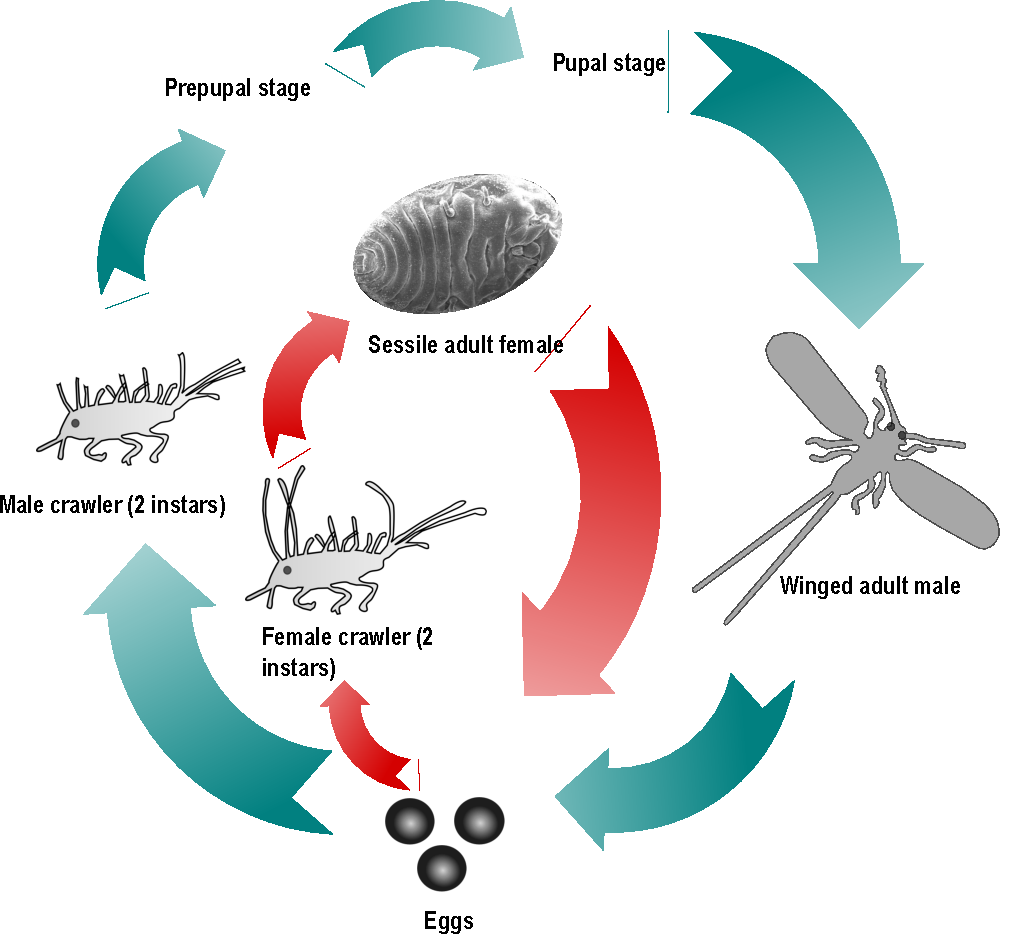
\includegraphics[scale = 0.5]{Images/lifecycle.pdf}
% 	\caption{Lifecycle of \textit{Dactylopius}. Adapted from \citet{Moran1979}}
% 	\label{fig:lifecycle}
% \end{figure}
\section{DNA and molecular barcoding}

\subsection{History and application}

Analogous to the Universal Product Codes (UPCs) found on commercial goods, genetic barcodes are created through the amplification and sequencing of short segments or gene regions of an organism\textsc{\char13}s genome - most commonly the mitochondrial cytochrome oxidase I (COI) gene in animals, and the chloroplast rbcL (RuBisCo large subunit) and matK (maturase k) loci in plants \citep{Hebert2003, CBOL2009, Floyd2010}. These unique signature sequences are used for identification and for phylogenetic analyses \citep{Hebert2003}. Mitochondrial genes are the preferred targets for barcoding initiatives due to their generally higher mutation rates compared to nuclear genes \citep{Drake1998, Ballard2004, Haag-Liautard2008}, their relatively low rates of recombination \citep{Piganeau2004}, and their high abundance in cells \citep{Waugh2007}. The COI marker is particularly useful because it displays low rates of insertions and deletions, and despite being a relatively conserved region, it can be used to differentiate between species; particularly in insects \citep{Hebert2003, Blaxter2004}. 
Although the concept of species identification using molecular techniques began in the 1980s, particularly regarding microorganisms \citep{Nanney1982, McAndrew1983, Anderson1985}, \citet{Arnot1993} first used the term `DNA barcode' in a study aiming to barcode isolates of the \textit{Plasmodium falciparum} Welch protozoan. The method gained popularity in 2003 \citep{Hebert2003, Hebert2003a}, and the Consortium for the Barcode of Life (CBOL) was founded the following year \citep{CBOL2009}. The Barcode of Life Database (BOLD) currently contains over 6 million genetic barcodes representing 215 000 animal, 69 000 plant, and 22 000 fungal species \citep{BOLD2019}.
Also referred to as `microgenomic identification', genetic barcoding relies on nucleotide diversity between organisms to group them taxonomically, or according to distinct haplotypes \citep{Hebert2003a}. It is based on the premise that interspecific variation is greater than intraspecific variation, referred to as the `barcoding gap' \citep{Hebert2003}. An arbitrary sequence divergence criterion suggested that species could be delineated at 3\% for insects, and 2\% and above for vertebrates \citep{Hebert2003}. 
DNA barcoding can serve as an efficient tool for taxonomists, and has a wide variety of cross-disciplinary applications \citep{Savolainen2005, Frezal2008, Valentini2008} (see Table \ref{tab:barcoding}).
A major advantage of genetic barcoding is its applicability to various stages of an organism's life cycle; as the genetic signature remains the same irrespective of differences in the individual's age \citep{Floyd2010}. 

\subsection{Caveats}

Despite the advantages, there are a number of criticisms of DNA barcoding, particularly with reference to its use as a standalone tool for the description of new species \citep{Rubinoff2006a}. The main arguments put forward include the the following: \vspace{0.4cm}
% \citet{Moritz2004DNAPitfalls, Will2004MythClassification,Rubinoff2005BetweenInference,Will2005,Cameron2006, Rubinoff2006, Rubinoff2006a, Frezal2008, Valentini2008, Pecnikar2014}. \\

\begin{enumerate}
    \item Heteroplasmy and differential inheritance of mitochondrial genomes.
    \item Maternal mitochondrial inheritance.
    \item Differential rates of gene evolution.
    \item Introgression of mitochondrial genes.
    \item Incomplete lineage sorting.
    \item The occurrence of nuclear mitochondrial DNA segments (numts).
\end{enumerate}

\subsubsection{Heteroplasmy}
Heteroplasmy in the mitochondrial genome refers to the presence of more than one genotype within an organism, such that there is a ratio of `mitotypes' (analogous to haploptypes); where one is often predominant over the others \citep{Kmiec2006}. Mitotypes can come about due to differences in nucleotide length (length heteroplasmy) or composition of mtDNA (site heteroplasmy) due to the insertion or deletion of large fragments, or errors in the replication process \citep{Barr2005}. New mitotypes can also be created following the exposure of mtDNA to oxygen metabolites, resulting in point mutations \citep{Kmiec2006}. Mitochondria are the vestiges of ancestral bacterial endosymbionts \citep{Gray1999} and replicate independently of the nucleus \citep{Meusel1993}. This unique system of genomic segregation and replication results in the differential transferal of mitochondrial genomes to daughter cells; facilitating heteroplasmy \citep{Barr2005}. 

\subsubsection{Maternal inheritance}
Although mitochondrial genomes are predominantly maternally inherited and rarely undergo recombination in animals, there are an increasing number of cases of biparental inheritance, or `paternal leakage', in which some mitochondrial sequences are inherited from males \citep{Gyllensten1991, Zouros1992, Skibinski1994, Hoarau2002, Kvist2003, Barr2005, Xiong2013, Ladoukakis2017}. This has been found in some insects, such as \textit{Drosophila simulans} Sturtevant (Diptera: Drosophilidae) \citep{Wolff2013} and \textit{Magicicada} spp. L. (Hemiptera: Cicadidae) \citep{Fontaine2007}. Additionally, `doubly uniparental inheritance' is another system that is common in bivalves, where male offspring inherit mtDNA from both parents while females inherit maternal mtDNA only \citep{Zouros1994}. The paternal transmission of mtDNA is usually prevented through a number of mechanisms across species, such as the destruction of male mitochondria in the developing zygote, the total absence of mitochondria in sperm, and the prevention of male mitochondria entering the oocyte upon fertilisation \citep{Rokas2003}. The process of paternal leakage, however, occurs more frequently in animals than was previously realised and can contribute to inconsistencies in the comparison of genetic barcodes. This is in addition to the growing understanding of the effects of mitochondrial bottlenecks during oogenesis \citep{Jenuth1996, Stewart2008} and the occurrence of mitochondrial recombination in some animals \citep{Piganeau2004, Rubinoff2006a}. \\
Since mitochondrial genomes are predominantly maternally inherited, the resulting sequences may be sex-biased \citep{Rubinoff2006a, Frezal2008, Innocenti2011}. Selection pressures that differentially affect males and females are therefore not taken into account, such as differences in motility \citep{Rubinoff2004}, feeding preference \citep{Hulcr2007}, and the occurrence of genetic diseases \citep{Frank1996, Camus2012}. Additionally, the barcoding of insects infected with \textit{Wolbachia} bacteria might lead to inaccuracies due to the effect that the symbionts have on reproductive functioning and the transferal of mitochondrial haplotypes in a population \citep{Gerth2011}. 

\subsubsection{Differential rates of gene evolution}
Analogous to the uncertainties of the differential rate of mutation in the use of molecular clocks \citep{Penny2005, Pulquerio2007, Weir2008}, the rate of evolution in the genes used for barcoding will vary between taxonomic groups \citep{Rubinoff2006a}. Mutation rates of genes in mitochondria are influenced by the unique asymmetrical mode of replication of the genome, where proximity to the site where replication begins is important \citep{Gibson2004}. The lagging strand remains single-stranded until about two thirds of the leading strand has been replicated, which renders it more susceptible to mutations \citep{Clayton2003, Rubinoff2006}. Genome arrangements are not necessarily consistent across taxonomic groups owing to the vast array of genetic systems in existence, and to factors such as life history strategies \citep{Rubinoff2006}. 
This could affect genetic barcoding through the size of the resulting barcode gap. A small or negative barcode gap results when there are too few mutational differences between groups to be able to tell them apart.

\subsubsection{Introgression of mitochondrial genes}
Introgression, also referred to as interspecific gene flow, is the incorporation of genes from the gene pool of one species into that of another through hybridisation and backcrossing \citep{Funk2003, Harrison2014}. This leads to polyphyly and the incongruence between gene and species trees \citep{Funk2003, Petit2009}. The introgression of mitochondrial genes used in barcoding initiatives can result in misleading conclusions, as taxonomic boundaries can become blurred \citep{Rubinoff2006, Petit2009, Ermakov2015}.
Mitochondrial introgression is particularly problematic due to limited recombination, resulting in the persistence of introgressed gene regions in a genome \citep{Funk2003}. An important assumption in analysing intra-and interspecific variation is that the study species are monophyletic with regards to the gene region of interest \citep{Funk2003}. \\
A number of studies have found that COI barcodes [alone] were unable to distinguish between species due to potential mitochondrial introgression and/or incomplete lineage sorting, such as in some cave-dwelling spiders (\textit{Circurina} spp.) (Araneae: Dictynidae) \citep{Paquin}, ground beetles (\textit{Carabus} L.) spp. (Coleoptera: Carabidae) \citep{Sota2001, Raupach2010}, African fruit bats (\textit{Pteropodidae} Gray) \citep{Nesi2011}, swallowtail butterflies (\textit{Papilio machaon} L.) (Lepidoptera: Papilionidae) \citep{Sperling1994}, and hairstreak butterflies (\textit{Calycopis} Scudder spp.) (Lepidoptera: Lycaenidae) \citep{Cong2017}. 

\subsubsection{Incomplete lineage sorting}
As with introgression, incomplete lineage sorting (or `deep coalescence') results in inconsistencies in topology between gene and species trees, such that the phylogeny of a particular gene does not match that of the species as a whole \citep{Maddison1997, Nichols2001,Funk2003}. Incomplete lineage sorting occurs when the coalescence of a gene back to a common ancestor pre-dates the speciation event (Fig. \ref{fig:gene_tree}) \citep{Maddison1997}. As such, the `sorting' of genes into the bifurcating lineages is not yet complete. 

\begin{figure}[H]
	\centering
	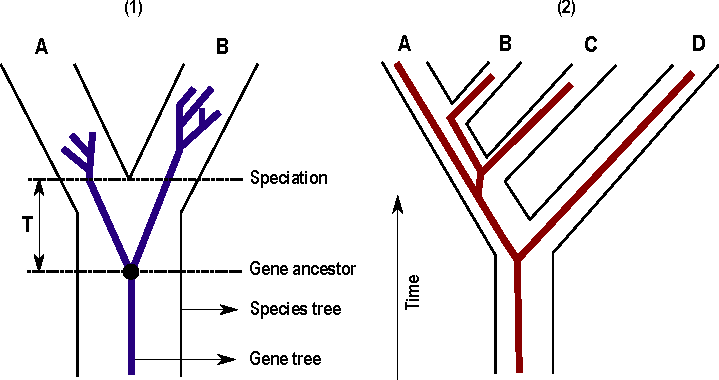
\includegraphics[scale = 1]{Images/gene_trees.pdf}
    \newline
	\caption{Gene trees within species trees, illustrating deep coalescence. (1) shows how the most recent common ancestor in the gene tree pre-dates that of the species tree by time T. (2) is another example of how the topology of a gene and species tree can differ. The species tree suggests that A and B share the most recent common ancestor, while the gene tree contrastingly shows that this is true for B and C. (Adapted from \citet{Maddison1997,Nichols2001,Edwards2009}).}
	\label{fig:gene_tree}
\end{figure}

\subsubsection{Nuclear mitochondrial DNA segments}
Nuclear mitochondrial DNAs (`numts'), also referred to as `pseudogenes', are non-functional gene regions that have translocated from the mitochondrial to the nuclear genome \citep{DErrico2004, Frezal2008, Hazkani-Covo2010, Leite2012}. Pseudogenes were first discovered in mice \citep{DuBuy1967} and locusts (\textit{Locusta migratoria} L.) (Orthoptera: Acrididae) \citep{Gellissen1983}, and have since been found to occur frequently across a wide range of taxa \citep{Lopez1994, Zhang1996, Williams2001, Richly2004, Pamilo2007}; particularly in plants and arthropods \citep{Gellissen1983, Bensasson2000, Bensasson2001, Buhay2009}. One of the most extreme examples was found in the domestic cat, where nearly half of its mitochondrial genome was present in the nucleus \citep{Lopez1994}! It is believed that the transfer of mitochondrial genes to the nucleus is a very ancient process, and that pseudogenes might arise due to unsuccessful transfers between the two organelles \citep{DErrico2004}. 
Pseudogenes are problematic in DNA barcoding because these regions can be co-amplified in addition to the target mitochondrial gene (identifiable by differences in nucleotide composition, the presence of indels, point mutations, and in-frame stop codons) \citep{Bensasson2001, Song2008, Moulton2010, Ahmed2015}. Depending on the accumulation of mutations (where mutation rates and selection pressures differ between the mitochondrial and nuclear genomes), conservative primers may preferentially amplify pseudogenes, resulting in paralogous sequences that have little comparative value and lead to the inference of incorrect phylogenetic relationships \citep{Bensasson2001, Song2008, Moulton2010, Leite2012}. To further complicate matters, the number of copies and composition of pseudogenes can vary between individuals, where multiple independent transferral events could have occurred over time \citep{Bensasson2000,Bensasson2001}. \citet{Song2008} found that the presence of pseudogenes in the COI barcodes for grasshoppers and crayfish lead to an overestimation of the number of species sampled by 2.8 and 3.6-fold, respectively. The authors concluded that the co-amplification of pseudogenes can be `disastrous' for DNA barcoding if sequences are not screened properly, and if only one gene marker is relied upon. \\
Despite the potential shortcomings of barcoding, the method has been successfully applied in numerous studies involving insects, representing groups such as the Heteroptera \citep{Raupach2014, Havemann2018}, Orthoptera \citep{Hawlitschek2017}, Lepidoptera \citep{Hausmann2013GeneticSystem, Razowski2017UncoveringTortricidae, Spitsyn2018DNAPleistocene}, Coleoptera \citep{Raupach2010, Hendrich2015ABOLD}, Diptera \citep{Lin2015ExploringBarcodes}, Ephemeroptera, Plecoptera, Trichoptera \citep{Cordero2017DNACanada,Cukusic2017DNACroatia}, and Hymenoptera \citep{Schmidt2017IdentificationCaveats}. If used appropriately, while remaining cognisant of its weaknesses, genetic barcoding can serve as a very valuable identification tool.
\section{Inter-simple sequence repeats (ISSRs)}

Inter-Simple Sequence Repeats (ISSRs) are sections of DNA located between microsatellites (=‘Simple Sequence Repeats’ (SSRs)) in an organism's genome \citep{Zietkiewicz1994, wolfe2005issr, Gaskin2011} (Fig. \ref{fig:issr}). Microsatellites are sequences of repeated DNA motifs that usually occur randomly at multiple loci in a genome, range from one to six nucleotides in length, and display a high mutation rate \citep{Gaskin2011, Hoy2013}. The ISSRs between these regions are particularly useful in detecting intraspecific variation due to their polymorphic nature \citep{Abbot2001}. In other words, each individual displays unique ISSR fragment sizes throughout their genome, which can be detected through the visualisation of banding patterns on an agarose gel and/or through capillary electrophoresis. ISSR primers typically consist of dinucleotide or trinucleotide base repeats \citep{wolfe2005issr}. ISSR analysis was developed in 1994, and was originally used to differentiate between plant cultivars \citep{wolfe2005issr}. Its application later extended to a wide range of other taxonomic groups, such as fungi \citep{kerrigan2003ascobotryozyma}, molluscs \citep{casu2005fine, casu2006inter}, birds \citep{haig2003parentage, wink2006use}, crocodiles \citep{machkour2009between}, snakes \citep{guicking2006introduced, nagy2007species}, lizards \citep{joger2007phylogeography}, tarantulas \citep{machkour2009issr}, sphingid moths (Lepidoptera: Sphingidae) \citep{hundsdoerfer2006incongruence}, the diamondback moth (\textit{Plutella xylostella} L.) \citep{roux2007issr}, lac insects (\textit{Kerria} spp.) \citep{saha2011genetic}, and silkworms (\textit{Bombyx mori} L.) \citep{chatterjee2003identification}. The technique has been used in the field of biological control in recent years, such as the genetic matching of invasive weeds to their native range \citep{paterson2013issrs, barker2015barcoding, Sutton2017GeneticAgents} and the detection of cryptic species \citep{Paterson2016} and genetic diversity \citep{Taylor2011GeneticMiridae} within the insect agent \textit{Eccritotarsus catarinensis} Carvalho (Hemiptera: Miridae), which is used for the biological control of water hyacinth. 
ISSR analysis is advantageous for the following reasons: \vspace{0.4cm}

\begin{enumerate}
    \item Primers are universal and can be used without prior knowledge of the target genomic sequence \citep{Wolfe1998, Gaskin2011}.
    \item ISSRs are abundant in the genomes of a wide variety of taxonomic groups and are highly informative and reproducible.
    \item The method is quick and cost-effective relative to other genotyping methods such as AFLP\textsuperscript{\textregistered} (amplified fragment length polymorphism) and RFLP (restriction fragment length polymorphism) \citep{Zietkiewicz1994, bornet2001nonanchored, bornet2004issr, DNAFragAnalysis}.
    \item The mutation rate of microsatellite regions is rapid \citep{wan2004genetic, DNAFragAnalysis}.
    \item Inherited microsatellite alleles are stable over multiple generations, and can be used at the population and individual level \citep{DNAFragAnalysis}.
\end{enumerate}

\subsection{Caveats of inter-simple sequence repeats}

\citet{meudt2007almost} state that AFLPs tend to outperform ISSRs and RAPDs (random amplified polymorphic DNA) in terms of lower genotyping error and higher robustness and informativeness. A number of studies involving crop cultivars and other plants have compared different fragment analysis methods, and many have supported this statement \citep{jones1997reproducibility, mcgregor2000comparative, hodkinson2002characterization, archak2003comparative, garcia2004comparison, behera2008relative, costa2016comparison}. \newline
Genotyping error refers to the differences between the genotypic data obtained independently from the same sample \citep{bonin2004track}.
The two overarching causes of such errors associated with `band-based' methods (including AFLPs and RAPDs) are allele homoplasy and scoring errors \citep{,bonin2004track, bonin2007statistical, holland2008optimizing}. 

\subsubsection{Homoplasy}
The term `homoplasy' means that the same characteristic has evolved independently in two or more otherwise different entities/species. Allele homoplasy thus refers to instances where fragments appear at the same position on a gel or an electropherogram, but are non-homologous \citep{bonin2007statistical, simmons2007penalty}. This phenomenon appears to increase in frequency in smaller fragments and in dense profiles, and when taxonomic distance increases; such that its effect on intraspecific comparisons is negligible \citep{bonin2007statistical}. Conversely, a particular locus may have undergone a mutation, insertion or deletion, resulting in the appearance of two or more independent loci that are actually linked \citep{simmons2007penalty}. \citet{simmons2007penalty} also mention the concerns around the origins of the amplified fragments (i.e. whether they are from the nuclear or mitochondrial genome, or whether they are in fact contaminants from hosts, parasites, or symbionts). 

\subsubsection{Error rates}
Data scoring is considered to be the main source of errors in fragment analysis procedures due to the high level of subjectivity involved at various stages of the analysis process \citep{bonin2004track}. Scoring errors for ISSRs can be largely overcome through the replication of each sample at the polymerase chain reaction (PCR) step. The most important determining factors in the comparison of replicate samples include:
\vspace{0.4cm}
\begin{enumerate}
    \item Differences in band intensity and what the peak height threshold is set at (i.e. what level of fluorescence is considered background noise, and how the number of false positive and negative calls can be minimised?).
    \item The bin width applied to score the presence and absence of bands (i.e. how strict or lenient should one be when determining whether a band occurs at the same locus in a replicate pair? What level of leeway should there be? If the bin width is too large, otherwise separate characters will be grouped as one, whereas a bin width that is too small will result in the scoring of numerous characters which are actually only representative of one locus) (Fig. \ref{fig:scoring_errors}). 
\end{enumerate}
\vspace{0.4cm}

\noindent Error rates are typically calculated as the average ratio between the number of mismatches and the total number of instances where a band was present, and absent, in both replicates (referred to as the Euclidean error rate) \citep{pompanon2005genotyping, bonin2007statistical}. It is suggested that an alternative error rate (the Jaccard error) should be calculated to complement the Euclidean error value. The Jaccard error calculation does not consider the shared absence of a band, as this absence may not be biologically meaningful \citep{holland2008optimizing}. AFLP Euclidean error rates typically range between 2 and 5\%, but \citet{bonin2007statistical} suggest that it should ideally not exceed 1\%. \citet{holland2008optimizing}, however, suggest that inter-study comparisons of error rates are not always reliable, as they encompass both PCR and scoring errors, and varying levels of divergence and data set size. Their study, for example, yielded AFLP error rates of 9 to 18\% and 6 to 13\% for sweet potato (\textit{Ipomoea batatas} (Convolvulaceae)) and \textit{Ourisia} (Plantaginaceae), respectively. Additionally, most of the studies reporting genotyping errors refer to AFLP techniques, and so it is unclear to what degree ISSR error rates are comparable. Surveys conducted by \citet{guichoux2011current} and \citet{bonin2004track} found that only between 6 and 26\% of papers, respectively, dealing with microsatellites reported error rates.  

\subsection{ISSRs as an identification tool}
Due to the significantly higher mutation rate in microsatellites compared to other DNA regions \citep{Zietkiewicz1994, Reddy2002}, ISSRs can offer higher resolution results that reveal greater differences between groups. This could be valuable in cases where traditional DNA barcoding regions are not sufficient in differentiating between closely related taxa, such as intraspecific lineages and different population groups. Fragment analysis methods, such as ISSRs, can therefore be used as molecular barcodes through the creation of unique fingerprint profiles (see for example \citet{galbacs2009identification}, \citet{adhikari2015efficiency}, \citet{li2018establishment}, and \citet{zhao2019molecular}).

\vspace{0.5cm}

\begin{figure}[H]
	\centering
	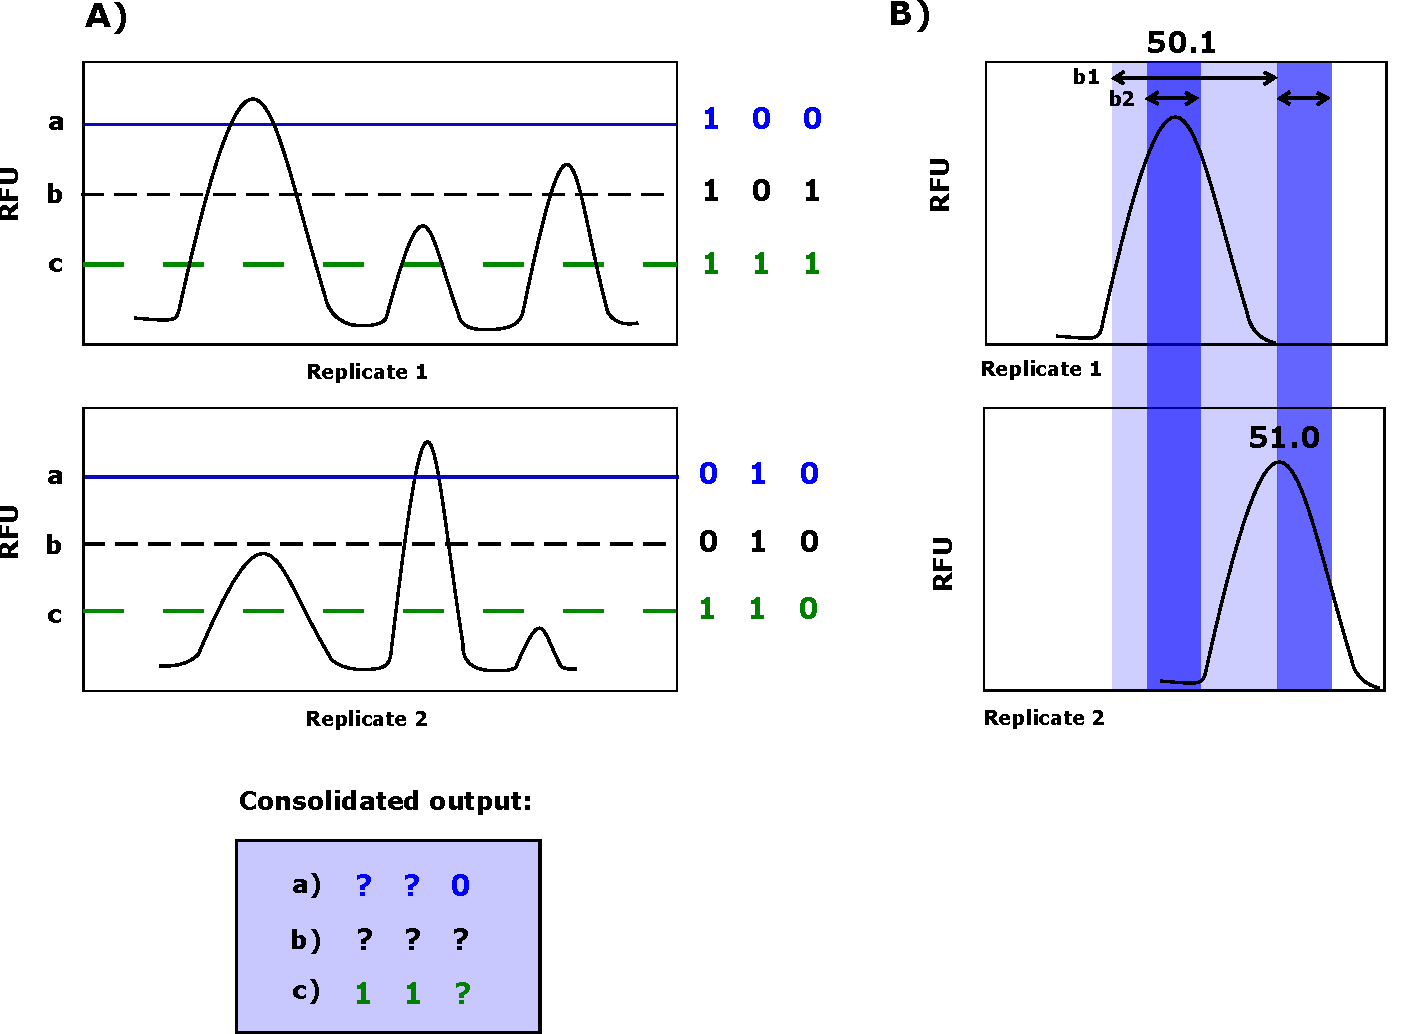
\includegraphics[scale = 0.7]{Images/source_of_scoring_errors.pdf}
	\caption{Potential sources of scoring errors in band-based genotyping methods: A) Determining the optimal threshold value to apply when scoring the presence or absence of a peak. The illustration shows three RFU (Relative Fluorescence Units) threshold levels (a, b and c), the resulting binary output at each, and the consolidated binary output representing a replicate pair (where a 1 and 0 or 0 and 1 outputs a `?', the shared presence of a band outputs a `1' and the shared absence a `0'). B) The effect of bin width on the scoring of peaks. Replicate 1 shows a band of 50.1 base pairs (bp) in size, and replicate 2 shows one of 0.9 bp larger. With a bin width set at b1, both will be scored as present at the same locus, but at a width of b2, these bands will be scored as two seperate loci.}
	\label{fig:scoring_errors}
\end{figure} 
\section{Aims}

The aims of this Master's thesis were to: 
\vspace{0.4cm}

\begin{enumerate}
    \item Obtain DNA and molecular barcode data to create phylogenies for the Dactylopiidae.
    \item Test the accuracy of these barcode databases.
    \item Develop protocols to allow for the accurate and quick identification of species, and more importantly, intraspecific lineages within \textit{Dactylopius opuntiae} and \textit{D. tomentosus}.
\end{enumerate}
\vspace{0.4cm}

\noindent To date, a number of distinct genetic lineages of \textit{D. tomentosus} have been determined (e.g. \citet{Mathenge2009, Mathenge2010}), but not for \textit{D. opuntiae} (namely the `ficus' and `stricta' lineages). Filling this knowledge gap is very valuable to the biological control of invasive Cactaceae around the world, and offers a number of important  practical applications. 



\chapter{Materials and Methods}
\label{sec:MaterialsAndMethods}
This document contains two appendices: A and B. Figures and Tables in Appendix A begin with the prefix `A', and Section numbers with `5'. 
The Figures and Tables in Appendix B begin with the prefix `B', and Section numbers with `6'. 

\section{Sourcing of samples}

\noindent Tables \ref{appendix:sequenceInfo} and \ref{appendix:issr_sample_table} contain detailed lists of all the samples used in this study. Outgroup and additional ingroup sequences were obtained from Genbank to supplement the dataset, and are listed in Table \ref{appendix:outgroups}.

\subsection{South Africa}

\subsubsection{Wild populations} 
\textit{Dactylopius opuntiae} samples were collected from wild populations on \textit{Opuntia ficus-indica} and \textit{Opuntia engelmannii} from various locations in the Eastern Cape Province. These are known to be the `ficus' lineage. 

\subsubsection{Uitenhage Mass Rearing Facility} 
 The Uitenhage Mass Rearing Facility in the Eastern Cape Province rears six insect agents for the control of invasive Cactaceae in the country. Four of these are \textit{Dactylopius} species, and were included in the analyses of this project. These were \textit{D. austrinus}, \textit{D. tomentosus} `imbricata', \textit{D. ceylonicus}, and \textit{D. opuntiae} `stricta' (more information is available at the Centre for Biological Control (CBC) Website, at \url{https://www.ru.ac.za/centreforbiologicalcontrol/massrearing/uitenhagemassrearingfacility/}). \\
As there are wild populations of the `ficus' \textit{D. opuntiae} lineage on \textit{O. ficus-indica} cacti in the surrounding vicinity, it is a concern as to whether this lineage is hybridising with the desired `stricta' lineage reared inside the facility. It is known that these two lineages can hybridise, which affects the host-specificity of offspring.
`Stricta' samples were collected from the facility and compared to original `stricta' source population samples and to `ficus' specimens to determine whether hybridisation had occurred. Individuals of the `stricta' lineage from the original stock imported from Australia were kept by Hildegard Klein and John Hoffmann (biological control specialists), and were used as a benchmark for the identification of this lineage.

\subsubsection{\textit{Dactylopius tomentosus} `cholla'} 
The \textit{Dactylopius tomentosus} `cholla' lineage was sourced from \textit{Cylindropunita fulgida} var. \textit{mammilata} in the Kirstenbosch Cape Town Botanical Gardens. Additional samples collected from \textit{C. fulgida} var. \textit{mammilata} in Jansenville in the Eastern Cape Province required identification confirmation, and were included in the analyses. 

\subsubsection{Kruger National Park}
\textit{Opuntia stricta} is the most widespread IAP in the Kruger National Park (KNP), covering approximately 35 000 ha surrounding Skukuza \citep{lotter1998integrated, foxcroft2004reconstructing}. It was first recorded in the Skukuza staff village in 1953, and spread rapidly within the subsequent decades \citep{lotter1998integrated}.
% Mechanical control attempts began in 1985 with the use of herbicides \citep{foxcroft2003Kruger}, but this was unsuccessful due to the survival of soil-stored seeds and small plants that had been overlooked, and the lack of follow-up work \citep{hoffmann1998long, foxcroft2004reconstructing}. 
% Biological control initiatives began in 1988 with the release of the phycitid moth \textit{Cactoblastis cactorum}, which provided a moderate level of control by stinting plant growth and reducing the time taken for plants to reach sexual maturity \citep{Hoffmann1998EvaluationAfrica, hoffmann1998long}.
\textit{Dactylopius opuntiae} was released on three separate occasions between 1990 and 1995, but did not establish on the weed \citep{lotter1998integrated, foxcroft2000dispersal}. This was because it was the `ficus' lineage, which does not establish on \textit{O. stricta} \citep{Volchansky1999}. The `stricta' lineage was subsequently imported from an Australian stock and released in the KNP in 1997, and has provided a substantial level of control \citep{lotter1998integrated, foxcroft2000dispersal}.
\textit{Dactylopius opuntiae} samples were obtained from Skukuza in the KNP in 2018 in order to confirm whether they were still of the original `stricta' lineage released in 1997. 

\subsection{Namibia}
\textit{Dactylopius opuntiae} samples were collected from \textit{O. ficus-indica} and \textit{O. stricta}. These were expected to be the `ficus' lineage, as this was the only lineage intentionally released in the country in 1975 and 1980 \citep{brown1985invasive, paterson2019prospects}. The first release in 1975 was for the control of \textit{O. stricta}, but the `ficus' lineage did not establish \citep{brown1985invasive} due to it being the incorrect agent. This is another example of the importance of correct identification. Additionally, two samples collected on an unidentified \textit{Harrisia} sp. in Windhoek were included in the present analysis. It was unexpected to find \textit{D. opuntiae} `ficus' on a \textit{Harrisia} cactus, and so further identification was required. 
\subsection{The USA}
\textit{Dactylopius} populations were collected from ten different \textit{O. engelmannii} lineages across the southern states of Arizona, New Mexico, Texas, and California in 2017 \citep{isbcw2018byrne}, and were identified morphologically as \textit{D. opuntiae}. These are currently in quarantine at the University of the Witwatersrand in Johannesburg, and are being tested for their use as additional biological control agents for \textit{O. engelmannii}. Samples from each lineage were included in the present genetic analysis.
Additional confirmed \textit{D. confusus} specimens were sourced from the Entomology Department at the University of Arizona, and included in the analysis for comparison. This is because \textit{D. opuntiae} and \textit{D. confusus} are frequently confused, as they are often found on the same individual host plant. Genetic analyses could therefore confirm the morphological identifications made for these ten lineages.

\subsection{Australia}
There are eight naturalised \textit{Cylindropuntia} species in Australia; namely \textit{C. fulgida} var. \textit{mamillata} ((D. C.) Backeberg), \textit{C. imbricata} (Haworth) F. M. Knuth, \textit{C. kleiniae} (D. C.) F. M. Knuth, \textit{C. leptocaulis} (D. C.) F. M. Knuth, \textit{C. prolifera} (Engelm.) F. M. Knuth, \textit{C. rosea} (D. C.) Backeberg, \textit{C. spinosior} (Engelm.) F. M. Knuth, and \textit{C. tunicata} (Lehm.) F. M. Knuth \citep{Jones2015}. All of these species negatively impact the environment, agricultural practices, and recreational activities \citep{Lloyd2014, Jones2015}. The Australians have imported 20 \textit{D. tomentosus} lineages into the country to serve as potential biocontrol agents \citep{isbcw2018Jones}, of which the `bigelovii', `acanthocarapa x echinocarpa', `cylindropuntia sp.', `imbricata', `cholla', and `californica' lineages
were obtained from Michael Day at the Department of Agriculture, Fisheries and Forestry, (Biosecurity Queensland) for inclusion in this project. These lineages are the most damaging to target weeds, and are in the process of, or have already been, released. Additional \textit{D. austrinus}, \textit{D. ceylonicus}, and \textit{D. opuntiae} specimens were included as well, which are commonly used biological control agents in Australia for Cactaceae, and have been established in the country for many years.

\subsection{Saudi Arabia}

\textit{Dactylopius opuntiae} samples collected from \textit{Opuntia stricta} were sourced from four localities in the Jazan Region of Saudi Arabia; namely Aldyer, Jazan City, Hurob, and Alaredah. Confirmation was required that these belonged to the `stricta' lineage, because this particular lineage provides the greatest level of control for \textit{O. stricta} weeds.

% Scanning electron microscope (SEM) images were taken of \textit{Dactylopius austrinus}, \textit{D. ceylonicus}, \textit{D. tomentosus} `imbricata' and `cholla' and \textit{D. opuntiae} `ficus' (images are in the \hyperref[appendix:semImages]{Appendix}). 

\section{Sample preservation and DNA extraction}
All specimens were preserved in 95\% ethanol and stored at -18\textsuperscript{o}C. Microscope slides of selected specimens were prepared according to the methods of \citet{Ben-Dov1997}. 
Buffer ATL (tissue lysis buffer) (Qiagen\textsuperscript{\textcopyright}) and Proteinase K (Qiagen\textsuperscript{\textcopyright}) were used to digest insect tissue, followed by a standard salt extraction procedure \citep{Bruford1992} (See Section \ref{appendix:extractionProtocol} for the detailed protocol). DNA pellets were resuspended in 100 $\mu$L AE (elution) buffer (Qiagen\textsuperscript{\textcopyright}) and stored at -18\textsuperscript{o}C. The concentration and purity of DNA extracts were ascertained through the use of a ThermoScientific Nanodrop 2000 spectrophotometer. When present, carminic acid residues in the extracts affected spectrometry and DNA concentration readings, but did not inhibit the successful amplification of target fragments.  

\section{DNA sequencing}

\subsection{Gene regions}

Three gene regions were amplified; namely the mitochondrial cytochrome oxidase subunit 1 (COI) region and 12S ribosomal (12S rRNA) region, and the nuclear 18S ribosomal (18S rRNA) region. 
% Mitochondrial DNA (mtDNA) is a double-stranded circular molecule ranging between 15 and 18 kb in length; containing 37 genes as well as non-coding regions \citep{Cameron2014InsectPhylogeny}. It makes up about 1 to 2\% of the total DNA in a cell \citep{Yang2014}. The coding gene region comprises of 13 protein coding, 22 transfer RNA (tRNA) and 2 ribosomal RNA (rRNA) genes \citep{Yang2014,Cameron2014InsectPhylogeny}. 
Mitochondrial DNA is maternally inherited, and is highly conserved across the insect orders and bilaterian animals as a whole \citep{Hoy2013, Cameron2014InsectPhylogeny}. This high level of conservation makes it particularly useful for phylogenetic studies \citep{Lunt1996, Hoy2013, DeMandal2014}. Another useful property of mtDNA is that different gene regions mutate at different rates, allowing for greater analytical potential \citep{Hoy2013}. 
% The COI mitochondrial gene encodes for the production of subunit 1 of the cytochrome c oxidase enzyme \citep{Lunt1996}. This enzyme plays an important role in cellular respiration by acting as both an electron transporter and translocator of protons across the cell membrane \citep{Lunt1996}. \citet{Yang2014} showed how conserved this gene is across organisms as disparate as humans and bacteria. 
The third position nucleotides of the COI gene display a high rate of base substitutions (`wobble'), leading to a mutation rate about three times faster than that of the 12S and 16S rDNA genes \citep{Knowlton1998}. This rapid rate of gene evolution has been found to be useful in using genetic barcoding to discriminate between phylogeographic lineages within the same species \citep{Cox2001, Gentekaki2012}. \\
% The 12S mitochondrial gene encodes for the production of rRNA, which translates mRNA into mitochondrial proteins \citep{Yang2014}. The 18S nuclear gene also encodes for the production of rRNA, which makes up the small ribosomal subunit \citep{Meyer2010}. 
The 18S gene is one of the slowest-evolving nuclear sequences, and is useful for assessing the ancestral relationships between organisms \citep{Hillis1991}. \citet{Campana2015} did not find any variation between the 18S markers across \textit{D. coccus} lineages, and hence discarded them from their study. The present study however used this gene because it involved a multi-species analysis.

\subsection{Polymerase Chain Reaction (PCR)}

Forward and reverse primers were used according to the methods of
\citet{Park2010RecoveryPrimers}, \citet{Campana2015}, and \citet{Mathenge2015} (Table \ref{tab:primers}). 

\vspace{0.5cm}

\begin{table}[H]
\renewcommand{\arraystretch}{0.6}
\centering
\caption{Primers used for the amplification of the COI, 12S, and 18S gene regions in \textit{Dactylopius} species.} 
\label{tab:primers} 
\begin{tabular}{@{}lll@{}}
\toprule
\multicolumn{1}{c}{\textbf{Gene}} & \multicolumn{1}{c}{\textbf{Primer pair (5' $\rightarrow$ 3')}} & \multicolumn{1}{c}{\textbf{Reference}} \\ \midrule
\multirow{4}{*}{\textbf{COI-A}} & \textbf{Forward (PcoF1)} & \citet{Park2010RecoveryPrimers} \\
 & CCTTCAACTAATCATAAAAATATYAG &  \\
 & \textbf{Reverse (LepR1)} &  \\
 & TAAACTTCTGGATGTCCAAAAAATCA &  \\ \hline
\multirow{4}{*}{\textbf{COI-B}} & \textbf{Forward (DTOMf )} & \citet{Mathenge2015} \\
 & TCCGRATAGAACTWATAAAYACYAA &  \\
 & \textbf{Reverse (HCO2198)} &  \\
 & TAAACTTCAGGGTGACCAAAAAATCA &  \\ \hline
\multirow{4}{*}{\textbf{12S}} & \textbf{Forward (12S-F)} & \citet{Campana2015} \\
 & AAGAGTGACGGGCRATTTGTACATA &  \\
 & \textbf{Reverse (12S-R)} &  \\
 & GTGCCAGCAGTWGCGGTTA &  \\ \hline
\multirow{4}{*}{\textbf{18S}} & \textbf{Forward (18S-F)} & \citet{Campana2015} \\
 & CTGGTTGATCCTGCCAGTAG &  \\
 & \textbf{Reverse (18S-R)} &  \\
 & CCGCGGCTGCTGGCACCAGA &  \\ \bottomrule 
\end{tabular}
\end{table}

\noindent The PcoF1 forward primer designed by \citet{Park2010RecoveryPrimers} binds upstream of the COI gene, in the tRNA domain, as this is a more conserved region. This increases the chance of amplification in groups that do not amplify with universal primers, as is generally found in the scale insects. This was true for the Dactylopiidae, as the universal HCO2198 and LCO1490 COI primers were tested here, and did not work for any species. \\
The two COI primer pairs used here (COI-A and COI-B) were checked to ascertain whether they amplify the same region of the COI gene by aligning representative sequences derived from each primer to the whole mitochondrial sequence of \textit{Ceroplastes japonicus} Green (Coccoidea: Coccidae) (Genbank ID: MK847519.1). Although they do amplify the same COI region, it was found here that COI-A only worked for \textit{D. confertus}, \textit{D. opuntiae}, and \textit{D. confusus}; while COI-B only worked for \textit{D. tomentosus}, as it was particularly designed by \citet{Mathenge2015} for this species. 
Samples were prepared according to the protocol in Table \ref{tab:PCRrecipe}, and amplified in a Bio-Rad T100 Thermal Cycler\textsuperscript{TM} set according to the protocol given in Table \ref{tab:PCRprotocol}.

\vspace{0.5cm}

\begin{table}[H]
\renewcommand{\arraystretch}{0.5}
	\centering
	\caption{PCR protocol for the 12S, 18S, COI-A, and COI-B genes in \textit{Dactylopius}.}
	\label{tab:PCRrecipe}
	\begin{tabular}{lcccc}
		\toprule
		\multicolumn{1}{c}{\textbf{Constituent}} & \multicolumn{3}{c}{\textbf{\begin{tabular}[c]{@{}c@{}}Quantity\\ ($\mu$L)\end{tabular}}} & \textbf{\begin{tabular}[c]{@{}c@{}}Concentration \end{tabular}} \\ \hline
		\begin{tabular}[c]{@{}l@{}}iTaq\textsuperscript{TM} Master Mix \end{tabular} & \multicolumn{3}{c}{12.5} & \multicolumn{1}{l}{} \\ 
		& \multicolumn{3}{c}{\textbf{Gene}} & \multicolumn{1}{l}{} \\ 
		& \multicolumn{1}{l}{\textbf{12S}} & \multicolumn{1}{l}{\textbf{18S}} & \multicolumn{1}{l}{\textbf{COI-A \& COI-B}} \\ 
		Forward primer & 3 & 3 & 2 & 10 $\mu$M \\ 
		Reverse primer & 3 & 3 & 2 & 10 $\mu$M \\ 
		ddH\textsubscript{2}O & 4.5 & 4.5 & 6.5 &  \\ 
		DNA sample & 2 & 2 & 2 & $\sim$50-150 ng/$\mu$L \\ 
		\textbf{Total} & \multicolumn{3}{c}{\textbf{25}} & \multicolumn{1}{l}{} \\ \bottomrule 
	\end{tabular}
\end{table}

\begin{table}[H]
\renewcommand{\arraystretch}{0.5}
	\centering
	\caption{PCR protocol for the 12S, 18S, COI-A, and COI-B genes.}
	\label{tab:PCRprotocol}
	\begin{tabular}{@{}clcc@{}}
		\toprule
		\textbf{Cycles} & \multicolumn{1}{c}{\textbf{Step}} & \textbf{Temperature (\textsuperscript{o}C)} & \textbf{Time} \\ \midrule
		1 & Initial denaturation & 94 & 5 min \\ \hline 
		\multirow{3}{*}{45} & Denaturation & 94 & 40 s \\ 
		& Annealing & 52 (12S); 58 (18S); 43 (COI-A); 50 (COI-B) & 35 s \\
		& Extension & 72 & 45 s \\ \hline 
		1 & Final extension & 72 & 10 min \\ \hline
		1 & Hold & 12 & $\infty$ \\ \bottomrule
	\end{tabular}
\end{table}

\noindent iTaq\textsuperscript{TM} Universal SYBR\textsuperscript{\textregistered} Green Supermix (Bio-Rad Laboratories Inc., USA) provided better amplification than TopTaq\textsuperscript{\textregistered} (Qiagen, Germany). The 12S, 18S, and COI genes yielded products approximately 450-500, 630-650, and 600-630 base pairs long. 
The 12S primers had a tendency to produce double bands for some samples (the target fragment plus a fragment approximately 1500 bp in size. See Fig \ref{fig:12Sgel}). Touchdown PCR (TD-PCR) was applied in such cases according to the protocol in Table \ref{tab:TDPCRprotocol}. 

\begin{table}[H]
\renewcommand{\arraystretch}{0.5}
\centering
\caption{12S Touchdown-PCR protocol that addressed double-band amplification.}
	\label{tab:TDPCRprotocol}
\begin{tabular}{@{}clcc@{}}
\toprule
\textbf{Cycles} & \textbf{Step} & \textbf{Temperature (\textsuperscript{o}C)} & \textbf{Time} \\ \midrule
1 & Initial denaturation & 94 & 5 min \\ \hline 
\multirow{3}{*}{5} & Denaturation & 94 & 30 s \\
 & Annealing & 54 & 30 s \\
 & Extension & 72 & 30 s \\  \hline
\multirow{3}{*}{35} & Denaturation & 94 & 30 s \\
 & Annealing & 51 & 40 s \\
 & Extension & 72 & 40 s \\  \hline
1 & Final extension & 72 & 8 min \\  \hline
1 & Hold & 12 & $\infty$ \\ \bottomrule
\end{tabular}
\end{table}

% \begin{itemize}
%     \item 1 cycle at 94\textsuperscript{o}C for 5 minutes
%     \item 5 cycles of 94\textsuperscript{o}C for 30 seconds, 54\textsuperscript{o}C for 30 seconds, 72\textsuperscript{o}C for 30 seconds
%     \item 35 cycles of 94\textsuperscript{o}C for 30 seconds, 51\textsuperscript{o}C for 40 seconds, 72\textsuperscript{o}C for 40 seconds
%     \item 72\textsuperscript{o}C for 8 minutes
%     \item 12\textsuperscript{o}C hold
% \end{itemize}


% \begin{table}[H]
% \renewcommand{\arraystretch}{0.5}
% \centering
% \caption{Primers used for the amplification of the COI, 12S and 18S genes in \textit{Dactylopius} species} 
% \label{tab:primers} 
% \begin{tabular}{ll}
% \toprule
% \textbf{Gene} & \textbf{Primer pair} \\ \hline
% COI & \begin{tabular}[l]{@{}l@{}}\\ \textbf{Forward (PcoF1):} \\ CCTTCAACTAATCATAAAAATATYAG\\ \textbf{Reverse (LepR1):}\\ TAAACTTCTGGATGTCCAAAAAATCA \\ \citet{Park2010RecoveryPrimers} \end{tabular} \\ \hline
% COI & \begin{tabular}[l]{@{}l@{}}\\ \textbf{Forward (DTOMf):} \\ TCCGRATAGAACTWATAAAYACYAA\\ \textbf{Reverse (HCO2198):}\\ TAAACTTCAGGGTGACCAAAAAATCA \\ \citet{Mathenge2015} \end{tabular} \\ \hline
% 12S & \begin{tabular}[l]{@{}l@{}}\\ \textbf{Forward (12S-F):}\\ AAGAGTGACGGGCRATTTGTACATA\\ \textbf{Reverse (12S-R):}\\ GTGCCAGCAGTWGCGGTTA \\ \citet{Campana2015} \end{tabular} \\ \hline
% 18S & \begin{tabular}[l]{@{}l@{}}\\ \textbf{Forward (18S-F):}\\ CTGGTTGATCCTGCCAGTAG\\ \textbf{Reverse (18S-R):}\\ CCGCGGCTGCTGGCACCAGA \\ \citet{Campana2015} \end{tabular} \\ \hline
% \end{tabular} 
% \end{table}

%\begin{figure}[h]
%	\centering
%	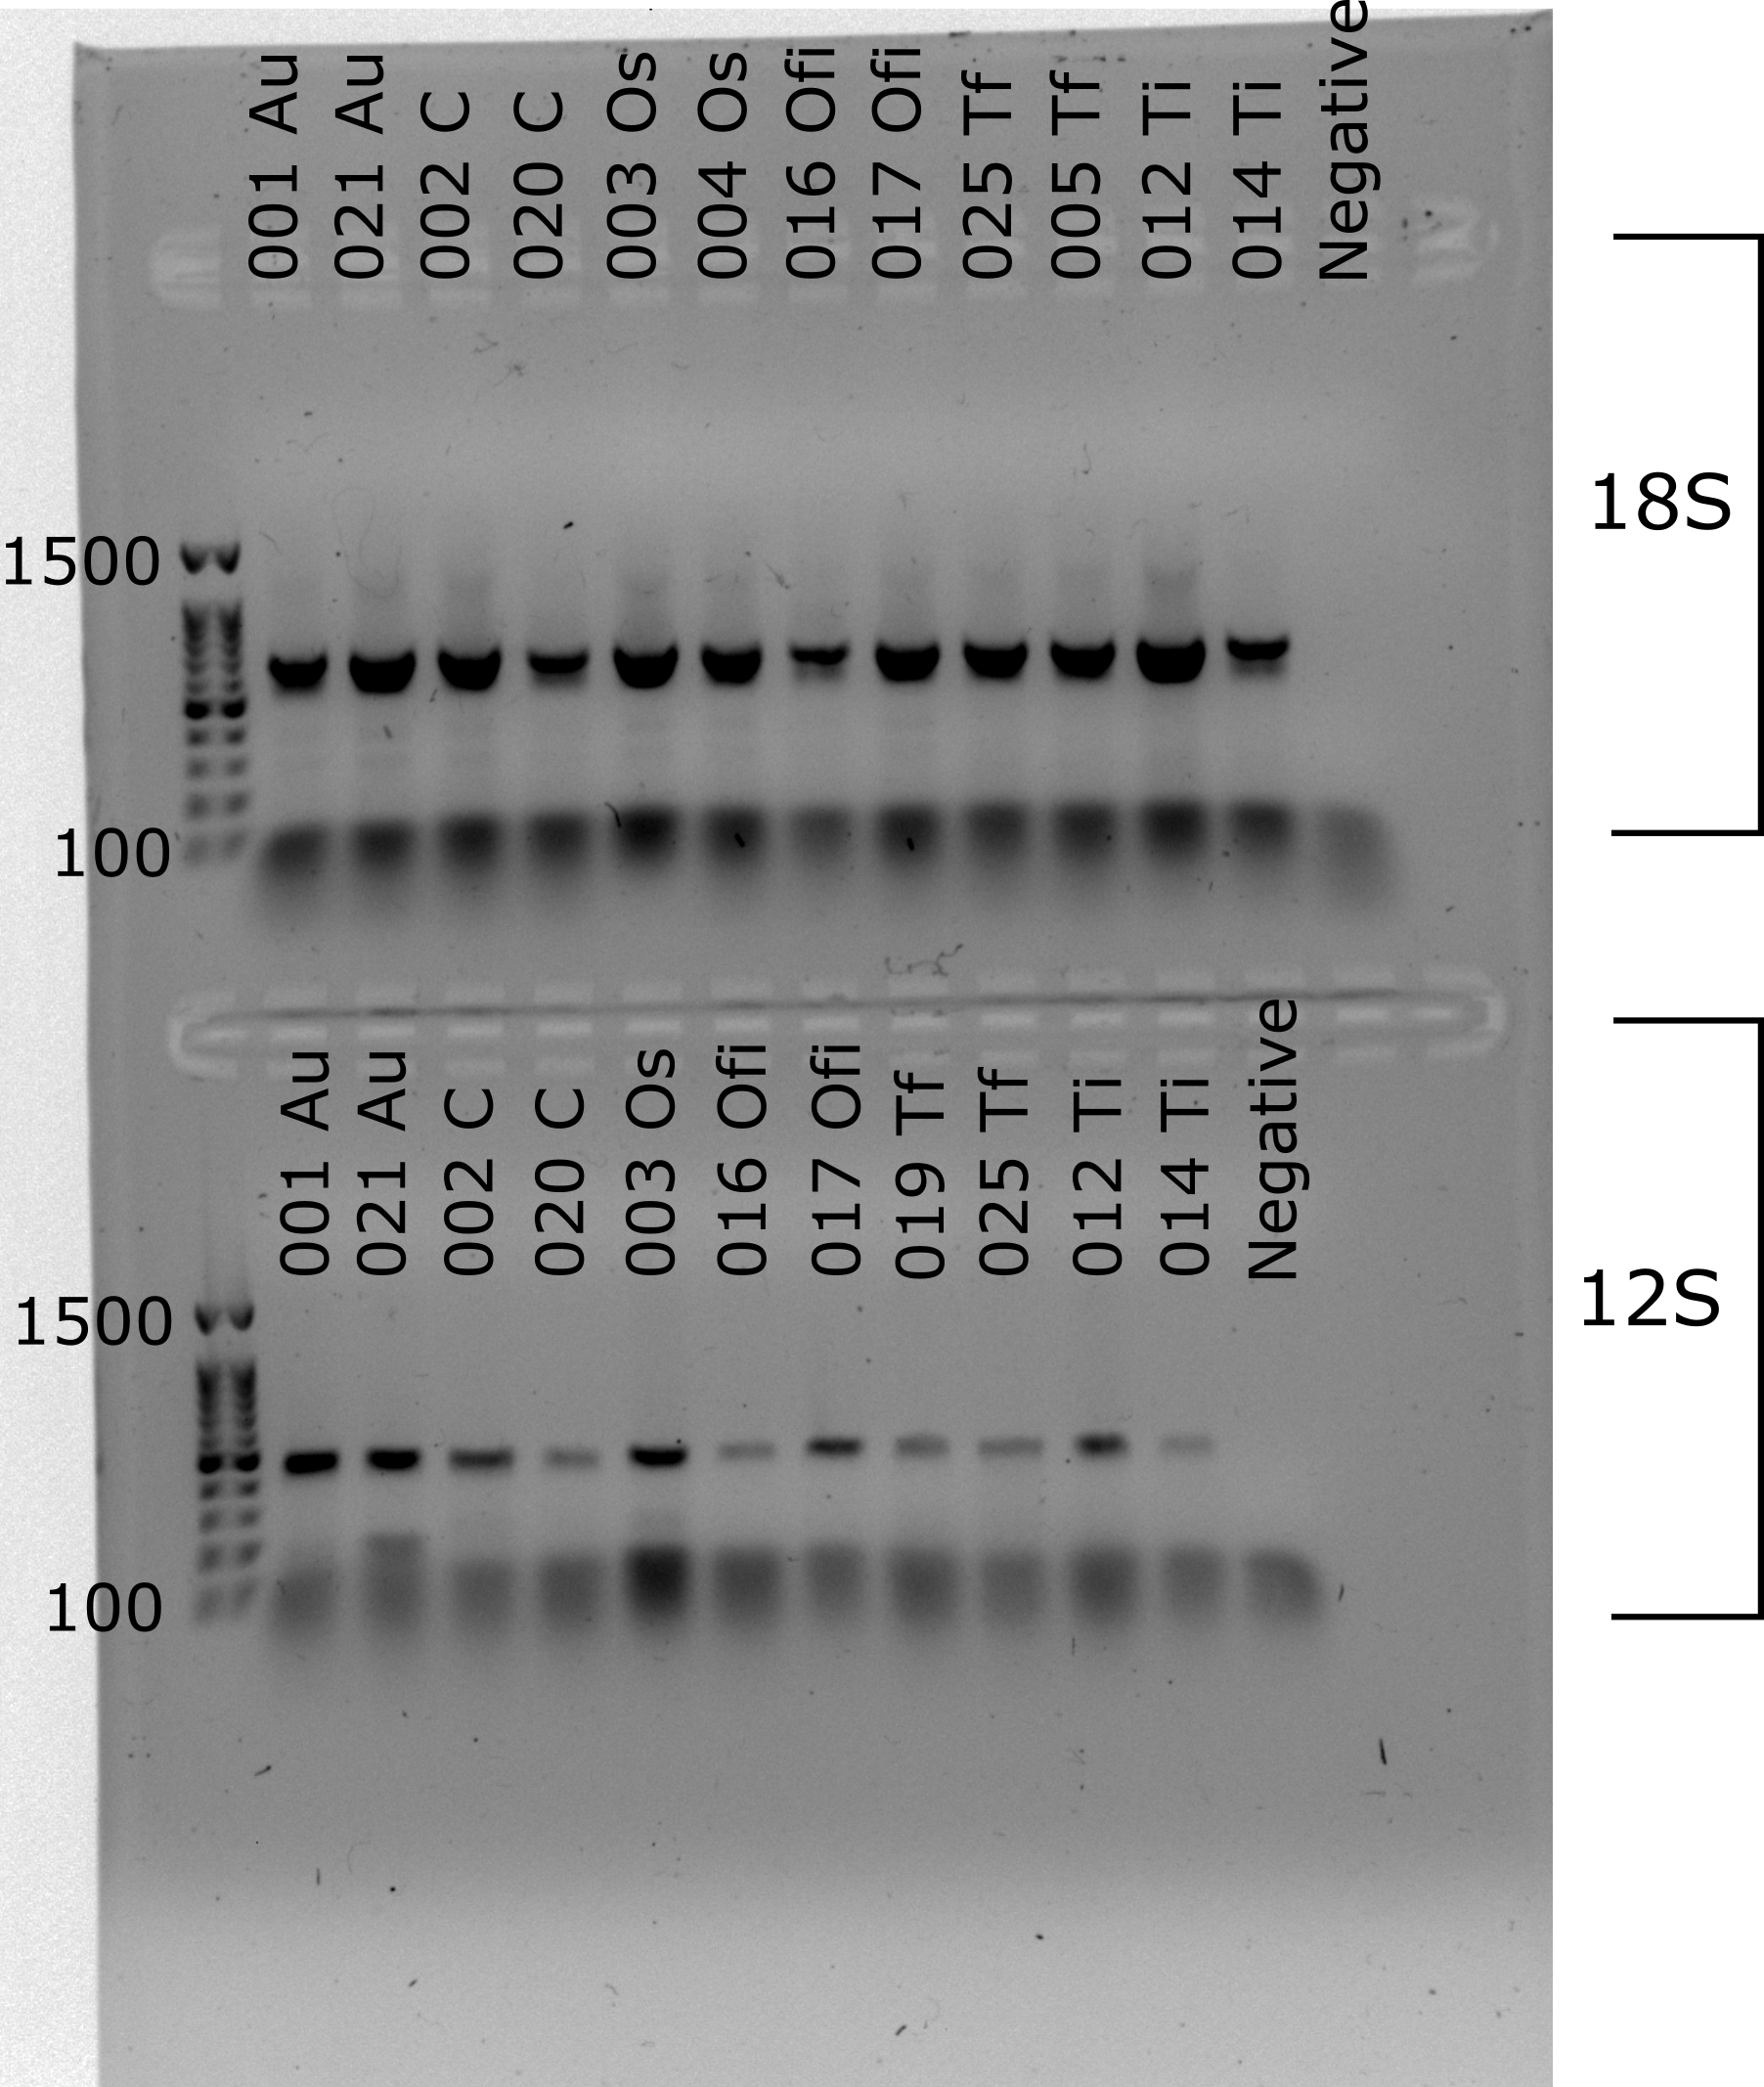
\includegraphics[scale = 1.3]{Images/12S_and_18S_gel}
%	\caption{Successful amplification of 12S and 18S genes}
%	\label{fig:gel1}
%\end{figure}

\subsection{Gel electrophoresis}
Gels were prepared using 100 mL TBE buffer (1X), 1 g Seakem\textsuperscript{TM} agarose (1\%) and 10 $\mu$L ethidium bromide. A 2 $\mu$L aliquot of loading buffer (PCRBIO Loading Buffer A) was added to 5 $\mu$L of each DNA sample. A 2 $\mu$L DNA ladder (PCRBIO Ladder IV, PCRBIOSYSTEMS) served as a standard. Gels were run at 90 V for 40 minutes using a Bio-Rad Powerpac\textsuperscript{TM}. Bands were visualized on a Bio-Rad Geldoc\textsuperscript{TM} molecular imager system and photographed using Image Lab\textsuperscript{TM} software. Amplified PCR products were sent to Macrogen Inc. in the Netherlands for purification, and for sequencing in the forward direction in all cases. 
% Relevant forward primer aliquots, diluted down to a concentration of 5 $\mu$M, were provided with the samples. 
% such that for n samples, n+5$\mu$L primer (at the original 10$\mu$M) was added to n+5 $\mu$L ddH\textsubscript{2}O.

\subsection{Sequence alignment}
Chromatograms were opened in Chromas v2.6.4 (Technelysium Pty Ltd.), where the beginning and ends of sequences were trimmed accordingly ($\pm$ 50 - 70 bp). These were subsequently opened in BioEdit v7.0.5 \citep{Hall1999BioEdit:95/98/NT}, and their base calls verified against their corresponding chromatograms. Sequences were aligned online using MAFFT v7 \citep{Katoh2017MAFFTVisualization}. The MAFFT alignment method was chosen based on the review by \citet{Morrison2006L.Purposes}, which found this method to be the most accurate and consistent compared to the ProAlign, ClustalW, T-coffee, Muscle, and Clustal methods. \\
As an additional analysis, the 12S rRNA sequences were aligned according to their predicted secondary structures using R-Coffee \citep{moretti2008, wilm2008} on the \href{http://tcoffee.crg.cat/apps/tcoffee/index.html}{T-Coffee server} \citep{notredame2000t, di2011t}. Sequences that did not show high consistencies were removed from the alignment. \\
Final sequences were submitted to Genbank via the online submission portal available at \url{https://submit.ncbi.nlm.nih.gov/}. See Section \ref{appendix:genbank_submission} for more details regarding the Genbank submission process.

\subsection{Construction of phylogenetic trees}
jModelTest v2.1.10 \citep{Guindon2003ALikelihood., Darriba2012JModelTestComputing} was used to select appropriate evolutionary models for the 12S, 18S, and COI gene regions, followed by the use of Bayesian Inference and Maximum Likelihood methods to create phylogenies for each. A concatenated phylogeny was made for the 12S and 18S regions. The COI region was not included in this concatenation, because it contained only 49\% of the sequences represented by the 12S and 18S datasets. A test concatenated phylogeny with all three genes did not show well-resolved clades within \textit{D. tomentosus}. \\
Maximum Likelihood \citep{Felsenstein1981EvolutionaryApproach} phylogenies were created using GARLI v2.01 \citep{zwickl2006genetic}, and Bayesian phylogenies were created using MrBayes v3.2.6 \citep{Huelsenbeck2001MRBAYES:Trees.} via the CIPRES Science Gateway portal \citep{Miller2010CreatingTrees} (\url{http://www.phylo.org/}). Trees were viewed in FigTree v1.4.3 and edited in Inkscape v0.92.3. 

\subsubsection{Bayesian Inference and Maximum Likelihood}

MrBayes was run using random starting trees, four chains (three hot and one cold) and set to 50 million generations. Trees were sampled every 1000 generations with a burnin of 1250 (see Section \ref{appendix:bayesblocks} for the MrBayes Nexus files used for each gene region). Tracer v1.7 was used to check for MCMC convergence \citep{rambaut2018posterior}. \\ 
% \begin{figure}[H]
% 	\centering
% 	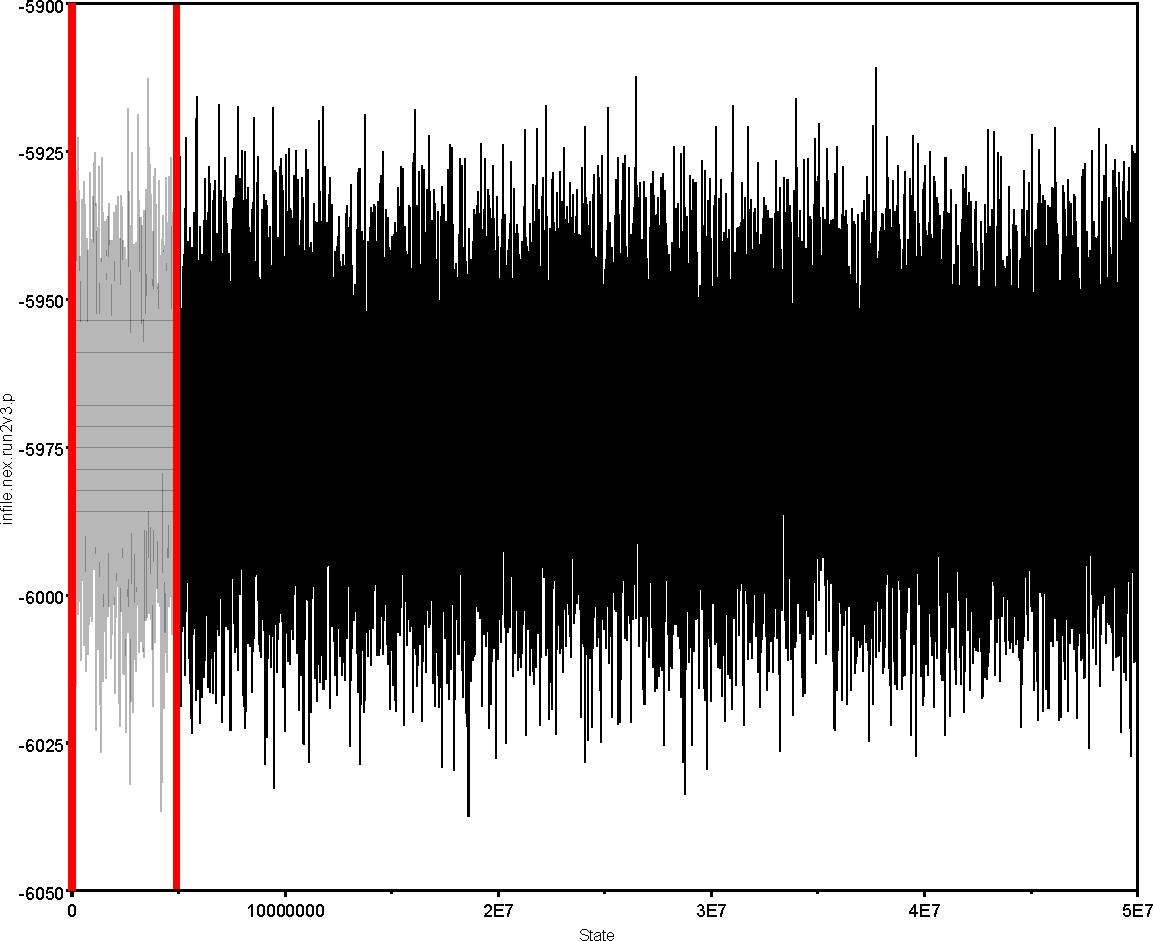
\includegraphics[scale = 0.32]{Images/tracer.pdf}
%     \newline
% 	\caption{An ideal tracer diagram indicating MCMC convergence. Burnin is the grey area between the two vertical red lines.}
% 	\label{fig:tracer}
% \end{figure}
Protein-coding COI sequences were assessed for substitution saturation at positions 1, 2, 3, and 1 \& 2 using the tests created by \citet{xia2003index} and \citet{xia2009assessing} in DAMBE v6 \citep{xia2018dambe7}. It is important to check for codon saturation, because the actual genetic distances in a dataset could be significantly underestimated due to multiple substitutions having taken place \citep{philippe2011resolving}. 
Sequences were ensured to be in the longest open-reading frame using BioEdit v7.0.5.3. 
% A significant p-value and an index of substitution saturation (ISS) less than the critical index of substitution saturation (ISSc) indicates little saturation, and that a partition model for that particular codon position is not required. 
GARLI and CONSENSE were used for the construction of Maximum Likelihood phylogenies via CIPRES. One thousand bootstrap repeats were run with two search repetitions. \\
Topologies of the individual gene trees for the 12S and 18S gene regions were compared using the online congruency index test `Icong', developed by \citet{devienne2007congruence}. To do this, a neighbour-joining tree was created for each gene region in MEGA v7 \citep{mega7} using the default settings. A significant p-value in `Icong' supports congruency, and thus the concatenation of the two relevant genetic datasets. 

\subsubsection{Haplotype networks in POPART}
POPART v1.7 \citep{leigh2015popart} was used to create 12S and COI haplotype networks for \textit{D. opuntiae} and \textit{D. confusus} using the TCS network method \citep{clement2000tcs}. \textit{Dactylopius tomentosus} haplotypes were not presented here because the 12S and COI phylogenies sufficiently represented the different lineages. It was, however, used to report the number of nucleotide differences between lineages of interest in this species. 
The 18S gene did not provide enough intraspecific variation, and was therefore not included. See Section \ref{appendix:popart} for the relevant file input formatting for POPART.
% The program was also used to calculate nucleotide diversity ($\pi$), the total number of segregating sites and Tajima's D statistic. 

\subsection{Distance-based testing of barcodes}
 The accuracy of barcode sequences were tested using the SPIDER package \citep{Brown2012Spider:Barcoding} in R v3.6.1 \citep{RCoreTeam2013R:Computing} at both the species and lineage level. This entailed the use of the Nearest Neighbour (NN), Threshold Identification (TID), and Best Close Match (BCM) methods. The threshold percentage used in TID was optimised to minimise cumulative error (false negatives + false positives). This was done by testing a range of threshold values from 0.0001\% to 2.5\% in increments of 0.005\% using the threshold optimisation function in the package. Pairwise distances were calculated using the K80 substitution model, using the dna.dist function in the R `Ape' package \citep{Paradis2004APE:Language}. The genetic barcoding gap was calculated and plotted using the SPIDER package by calculating the largest intraspecific and the smallest interspecific genetic distance for each sequence \citep{Meier2006DNASuccess}. See Section \ref{appendix:RCODE,SPIDER} for the R code used to implement these tests.
 
\subsubsection{Nearest Neighbour (NN)}
The NN algorithm was used to compare the genetic distance of each sequence of interest (treating it as a query sequence) to every other sequence in the relevant dataset. This method found the sequence that was most similar to it, and then checked whether this most similar sequence was conspecific or not. This was based upon the predefined species names, which returned a `true' or `false' result. In this way, the accuracy of each species' identification was tested and converted into a percentage of positive and negative outcomes. 

\subsubsection{Threshold ID (TID)}
The TID algorithm was used to find all the sequences that were within a genetic distance threshold of the query sequence, and returned `correct', `incorrect', or `no id' based on whether those matches were conspecific to the query sequence or not. The distance threshold was 1\% by default, but was set to an optimal value that minimised false positive and false negative results. 

\subsubsection{Best Close Match (BCM)}
The BCM algorithm was used in addition to the NN and TID, but instead of narrowing down all the matches within the genetic distance threshold, it only compared to the single nearest neighbour. It also returned `correct', `incorrect', or `no id' as output. The ambiguous output `no id' was returned when more than one sequence matched the query, where these matches included both conspecific and allospecific individuals. 
\subsubsection{Scoring of the barcode algorithms}
As per the methods of \citet{Birch2017TestingAustralia} and the R SPIDER documentation \citep{Brown2012Spider:Barcoding}, species and lineage identifications were considered: 
\vspace{0.4cm}

\begin{enumerate}
    \item ``True" in NN when the closest individual to the query was conspecific,  and ``correct" in BCM and TID analyses when all individuals with the closest distance to the query were conspecific and fell within the threshold applied.
    \item ``Ambiguous" in BCM analyses when different allospecific individuals shared the closest distance to the query and were within the threshold value or in TID analyses when different allospecific individuals were within the threshold value.
    \item ``No identification" in BCM and TID analyses when individuals were genetically more distant to the query than the threshold value.
    \item ``False" in NN when the closest individual to the query was allospecific, and ``incorrect" in BCM analyses when allospecific individuals shared the closest distance to the query and were within the threshold value or in TID analyses when all individuals within the threshold value were allospecific.
\end{enumerate}
\vspace{0.4cm}

\section{Inter-simple Sequence Repeats (ISSRs)}

\subsection{PCR protocol, data capturing and data processing}

Universal ISSR primers 809 (5'- AGA GAG AGA GAG AGA GC - 3') and 826 (5'- ACA CAC ACA CAC ACA CC -3') from Primer set \# 9 of the University of British Columbia Nucleic Acid Protein Service Unit  were used \citep{Abbot2001}. These were labelled with 5'6-FAM\textsuperscript{TM} fluorescent dye. PCRs were run in 20 $\mu$L reactions, consisting of 10 $\mu$L iTaq\textsuperscript{TM}, 1.5 $\mu$M primer and 1 $\mu$L DNA template (50 - 150 ng/$\mu$L). The PCR protocol was adapted from that of \citet{saha2011genetic} and \citet{silva2013genetic}, and carried out as per Table \ref{tab:PCRprotocol_ISSR}. 
A replication of each sample was conducted in a different PCR machine in order to validate the occurrence of bands/peaks \citep{Taylor2011GeneticMiridae, Sutton2017GeneticAgents}. As a preliminary validation step, 5 $\mu$L PCR product was run on a 1.5\% agarose gel at 6 V/cm for 3 hours (Fig. \ref{fig:issrGel}).
Samples were subsequently sent to the Central Analytical Facilities (CAF) division in Stellenbosch, South Africa, where DNA fragment analysis was performed using capillary electrophoresis (Applied Biosystems Inc., 3130 genetic analyser, GS500LIZ size standard).

\vspace{0.5cm}

\begin{table}[H]
\renewcommand{\arraystretch}{0.5}
	\centering
	\caption{PCR protocol for the ISSR 809 and ISSR 826 primers for \textit{Dactylopius} spp.}
	\label{tab:PCRprotocol_ISSR}
	\begin{tabular}{@{}clcc@{}}
		\toprule
		\textbf{Cycles} & \multicolumn{1}{c}{\textbf{Step}} & \textbf{Temperature (\textsuperscript{o}C)} & \textbf{Time} \\ \midrule
		1 & Initial denaturation & 95 & 7 min \\ \hline 
		\multirow{3}{*}{38} & Denaturation & 95 & 45 sec \\ 
		& Annealing & 44 (ISSR 809); 48 (ISSR 826) & 45 sec \\
		& Extension & 72 & 2 min \\ \hline 
		1 & Final extension & 72 & 7 min \\ \hline
		1 & Hold & 12 & $\infty$ \\ \bottomrule
	\end{tabular}
\end{table}

\subsection{ISSR data processing and analysis}

% \textbf{Summary: \newline \newline 
% \fbox{\parbox{\textwidth}{%
% Electropherograms uploaded to GeneMarker\textsuperscript{\textregistered} $\rightarrow$ Filtering of peaks above a 50RFU threshold $\rightarrow$ Creation of a peak summary table $\rightarrow$ Exportation to RawGeno for further filtering (100 RFU threshold) and binning (0.5-1bp) $\rightarrow$ Exportation of a binary matrix $\rightarrow$ Consolidation of ISSR replicates $\rightarrow$ Conversion of the binary matrix to a distance matrix using Jaccard's transformation $\rightarrow$ Creation of a hierarchical clustering dendrogram (UPGMA method) and nMDS plot in R and a NeighborNet tree in SplitsTree $\rightarrow$ Importation of the binary matrix into STRUCTURE to assess distinct genotypic clusters $\rightarrow$ STRUCTURE SELECTOR to find the optimal K-value (the best estimate of the number of genotypic clusters) $\rightarrow$ CLUMPAK (CLUster Markov Packager Across K) to visualise results as histograms.}
% }}
% \newline 
\subsubsection{Electropherograms to binary data}
Electropherograms were analysed in Genemarker\textsuperscript{\textregistered} v2.7.4 (SoftGenetics\textsuperscript{\textregistered}) (Fig. \ref{fig:overlay_electro}). 
See Section \ref{appendix:genemarker_settings} for more details regarding the settings applied.
Binary data from GeneMarker\textsuperscript{\textregistered} were opened in RawGeno v2.0 \citep{arrigo2012automated}. The following parameters were found to be the most efficient, while remaining conservative: 
\vspace{0.4cm}
\begin{enumerate}
    \item Maximum and minimum bin width of 1 and 0.5 base pairs (bp), respectively.
    \item Scoring from 100 to 500 bp.
    \item Low relative fluorescent units (RFU) of 100, as recommended by \citet{DNAFragAnalysis} for data produced by 3130 Series instruments.
\end{enumerate}
\vspace{0.4cm}

\noindent The resulting binary matrix was organised in Microsoft Excel\textsuperscript{\textregistered} and converted to a pairwise distance matrix in R using Jaccard's distance transformation. This transformation was applied because it does not consider the shared absence of bands as being biologically meaningful (Fig. \ref{fig:jaccard}) \citep{jacc}. See Section \ref{appendix:RCODE,Jaccard} for the relevant R code used to calculate distance matrices applying Jaccard's transformation. The Jaccard's distance (dJ\textsubscript{i}), and similarity (J\textsubscript{i}) index calculations are shown below, where f\textsubscript{11} represents the total number of times that a band occurred at the same place in both samples, f\textsubscript{00} represents the shared absence of bands, and f\textsubscript{10} and f\textsubscript{01} represents the number of times that a band was present in only one of the two sample replicates. Jaccard's distance is equal to 1 - Jaccard's similarity (J\textsubscript{i}). 
\vspace{0.4cm}

\[dJ\textsubscript{i} = \frac{f\textsubscript{01} + f\textsubscript{10}}{f\textsubscript{01} + f\textsubscript{10} + f\textsubscript{11}} = 1 - J\textsubscript{i} \] 

\[J\textsubscript{i} = \frac{f\textsubscript{11}}{f\textsubscript{01} + f\textsubscript{10} + f\textsubscript{11}} \] 

\subsubsection{Grouping methods}
The transformed distance matrix was subsequently used to create a hierarchical clustering dendrogram using the unweighted pair group method with arithmetic mean (UPGMA, 1000 bootstraps) using the `pvclust' R package \citep{suzuki2006pvclust}. See Section \ref{appendix:RCODE,upgma} for the R code used to construct this dendrogram. Further ISSR clustering and statistical analyses were applied to the \textit{Dactylopius opuntiae} `ficus' and `stricta' lineages in particular, as the traditional DNA barcoding regions could not differentiate between them.
Kruskal's non-metric multidimensional scaling (nMDS) method was applied using the isoMDS function in the MASS package in R \citep{MASS_R}. See Section \ref{appendix:RCODE, nmds} for the relevant R code used to create the nMDS plot. Dimensions K = 2 and K = 3 were tested, and the one yielding the lowest stress value was selected. The use of an nMDS ordination method was confirmed using stress and Shepard plots. 
% A stress plot shows how the number of dimensions of an MDS ordination affects the stress value, which is a measure of goodness of fit. The lower the stress value, the better the fit \citep{clarke1993}. A Shepard plot illustrates the relationship between the distance data before and after the ordination method has been applied. Ideally, the resulting regression should yield a high R\textsuperscript{2} value and show a significant correlation. \newline
An ANOSIM (ANalysis Of SIMilarity) was applied to lineages and populations using the `vegan' package in R \citep{vegan_R}, using 999 permutations \citep{clarke1993}. Pairwise p and R-values were obtained from PAST v3 \citep{Hammer2001PAST:Analysis}. 
% where a large positive R-value indicates a high level of dissimilarity, and a smaller value indicates increasing similarity. 
In addition to the ANOSIM, a Permutational Multivariate Analysis Of Variance (PERMANOVA) using distance matrices was used, applying the adonis function in the `vegan' package, with 999 permutations. This test is less sensitive to within-group heterogeneity \citep{anderson2014permutational}. Post-hoc pairwise comparisons were obtained via the pairwise.perm.manova function in the `RVAideMemoire' package \citep{herve2015rvaidememoire}. See Section \ref{appendix:RCODE,anosim,permanova} for the R code used to output the ANOSIM and PERMANOVA test results. \\
Data were also imported to SplitsTree4 v4.15.1 \citep{huson2006splitstree}, and used to create NeighborNet trees based on distance matrices that were transformed using Jaccard's distance index. NeighborNet trees were chosen because \citet{huson2006splitstree} suggest that this method produces highly resolved networks. See Section \ref{appendix:splitstree_input} for the SplitsTree file input format. 

\subsubsection{STRUCTURE}
STRUCTURE v2.3.4 \citep{Pritchard2000InferenceData, evanno2005detecting} was used to analyse the genetic clustering of \textit{D. opuntiae} samples. 
% This particular species was used because the traditional DNA markers did not show a separation between the `ficus' and `stricta' lineages. 
The program uses Bayesian analysis and the Markov Chain Monte Carlo (MCMC) estimation method to assign individuals to genotypic cluster groups (\textit{K}) \citep{Pritchard2000InferenceData}. 
% The method assumes that the input loci are in Hardy-Weinberg and linkage equilibrium, and does not consider any particular underlying mutation processes \citep{structureManual2009}.
STRUCTURE was run twice; once where the population origins for samples were given as priors (`PopData'), and once where they were not. 
% This was done through selecting the `use sampling locations as prior' option in the parameter settings.
See Section \ref{appendix:structure_settings} for details regarding the specific settings used. 
The results obtained from STRUCTURE were uploaded to STRUCTURE SELECTOR \citep{li2018structureselector}, which finds the best estimate of the number of genetic cluster groups (\textit{K}-value) present. The Peuchmaille method was preferred for this analysis, as it was found to outperform previous methods for datasets containing both even and uneven sample sizes \citep{puechmaille2016program}. \citet{puechmaille2016program} developed four statistical tests to estimate the optimal \textit{K}-value for a dataset, namely `MedMeaK', `MaxMeaK', `MedMedK', and `MaxMedK'. 
% The algorithm calculates mean and median membership coefficient values for each sample, compares it to a threshold (where a higher threshold implements a higher stringency), and assigns it accordingly to a cluster group. The mean and median number of cluster groups are subsequently estimated. 
The present analysis set the threshold to range between 0.5 and 0.8, as per the recommendations of \citet{puechmaille2016program}. The \textit{K}-estimation according to the conventional Evanno method \citep{evanno2005detecting} was also reported. CLUMPAK software \citep{Kopelman2015} was used to visualise results. 

% \subsubsection{POPGENE}
% POPGENE \citep{yeh1997population} was used to calculate the total number of alleles (na), effective number of alleles (ne), Nei's genetic diversity (h), Shannon's information index (I), polymorphic loci, total genetic diversity (Ht), intra population genetic diversity (Hs) and the coefficient of gene differentiation (Gst) for \textit{D. opuntiae} samples. This was done for each individual primer, as well as for their concatenation. See Section \ref{appendix:popgene_input} for details regarding the file input format.

\subsubsection{ISSR error rates}

Two genoytyping error rates were calculated, namely the `Euclidean' (EE) and `Jaccard' (JE) errors, as suggested by \citet{bonin2004track}, \citet{pompanon2005genotyping}, and \citet{holland2008optimizing}. \newline 
\[EE = \frac{f\textsubscript{10} + f\textsubscript{01}}{f\textsubscript{10} + f\textsubscript{01} + f\textsubscript{11} + f\textsubscript{00}} \] 
 
\[JE = \frac{f\textsubscript{10} + f\textsubscript{01}}{f\textsubscript{10} + f\textsubscript{01} + f\textsubscript{11}} \]
 
\noindent Due to the JE not taking the shared absence of bands into account, it will be inflated if the data contain numerous band-absent loci.

\section{Graphical User Interface (GUI) Applications}

\subsection{R Shiny Applications}
R Shiny applications \citep{shiny} are hosted on Amazon's Web Services online platform, and the front end can be accessed by any user via a unique url link. Running the program only requires an Internet connection, and does not rely on any pre-installed R software or related packages. Each Shiny application comprises of a user interface object (ui.R) and a server function (server.R), which are uploaded to a profile on \url{https://www.shinyapps.io/}. Three such applications were created and are described below. A help file accompanies each application. 

\subsection{Barcode Testing}
An application that allows a user to apply barcode testing algorithms to a set of aligned FASTA sequences (Fig. \ref{fig:barcodeTesterGUI}) is available at \url{https://clarkevansteenderen.shinyapps.io/BarcodeTester/}. The barcode tests were taken from the SPIDER package developed by \citet{Brown2012Spider:Barcoding}. The user can also view and download a heat map representation of a distance matrix, plots for base frequencies and GC content (using the `Ape' package \citep{Paradis2004APE:Language}), and a UPGMA clustering tree in the case of binary data.  

\subsection{Binary data processing: `BINMAT'}
A second GUI application (Fig. \ref{fig:binmatGUI}) was created in order to rapidly consolidate replicate pairs in a binary matrix containing fragment analysis data from a dominant genetic marker such as an ISSR or AFLP analysis (i.e. it requires already-scored data from a program such as GeneMarker\textsuperscript{\textregistered}). The algorithm combines replicates such that if a band was only present in one replicate (``0'' and a ``1''), it is treated as ambiguous (scored as a ``?''). The dual presence or absence of a band remains a ``1'' or ``0'', respectively. The application also calculates the average Euclidean and Jaccard error rates with standard deviations, and outputs the average, minimum, and maximum number of peaks and their standard deviations. An option is provided for constructing a UPGMA clustering tree to preview the clustering pattern of the data.
An additional feature allows the user to upload their consolidated matrix to create an interactive nMDS plot that can be downloaded as a .svg file. Options are available to view scree and Shepard plots for the data, download the distance matrix, and remove samples with total peak numbers below a specified threshold value. These filtered datasets can be downloaded and re-uploaded to create new nMDS plots. 
The BINMAT application is accessible at \url{ https://clarkevansteenderen.shinyapps.io/BINMAT/}.

\subsection{Identification of query sequences: `Dacty-ID'}

The third GUI application allows the user to paste a query nucleotide sequence into a search box, which is then aligned with sequences in a pre-selected database (Fig. \ref{fig:identifier_GUI}). The databases are the sequences for the 12S, 18S, and COI gene regions (COI-A and COI-B) obtained in this project. Alternatively, the user can upload their own set of sequences to serve as a database. A phylogenetic tree is subsequently created, where the position of the query sequence is highlighted in red relative to the database. The Dacty-ID application is available at
\url{ https://clarkevansteenderen.shinyapps.io/Dactylopius_ID_version_1/}. 

\chapter{Results}

\section{Codon saturation}

The COI gene region displayed little saturation at all codon positions (Table \ref{tab:saturation} and Fig. \ref{fig:COI_saturation_graphs}). This meant that additional codon models were not necessary in the construction of the COI phylogeny.
% See Figures \ref{fig:pcof1_saturation} and \ref{fig:co1_dtom_saturation} for the saturation graphs.

\section{Phylogenies}

\subsection{12S}
Sequence lengths were approximately 413 bp, with mean nucleotide base frequencies of A (44.57 $\pm$ 2.47\%), C (12.79 $\pm$ 1.74\%), T (38.11 $\pm$ 2.42\%), and G (4.54 $\pm$ 2.08\%). The optimal model used was GTR + G.
The 12S gene region provided well supported clades for all the \textit{Dactylopius} species included in the analysis, and for three of the six lineages within \textit{D. tomentosus} (Fig. \ref{fig:12S_tree}). The `echinocarpa x acanthocarpa', `bigelovii', and `cylindropuntia sp.' lineages grouped together as one clade. There were only two nucleotide differences between `bigelovii' and `echinocarpa x acanthocarpa', and one nucleotide difference between the latter and `cylindropuntia sp.'. The \textit{D. opuntiae} `ficus' and `stricta' lineages did not show any separation. 
See Figure \ref{fig:12S_rcoffee} for the resulting Bayesian tree produced from sequences aligned according to their secondary structure.
The samples collected from an unidentified \textit{Harrisia} sp. in Windhoek, Namibia, did not successfully amplify using this marker. 
The \textit{D. ceylonicus} clade showed a well-supported split between the South African and Australian samples. 
The Bayesian and Maximum Likelihood trees showed the same overall topologies, but the posterior probability and bootstrap support values differed quite substantially for some clades. For example, the split between the \textit{D. tomentosus} `californica' and `echinocarpa x acanthocarapa'/`bigelovii'/`cylindropuntia' lineages showed a posterior probability support of 0.8, but a bootstrap support value of only 47. Similarly, the split between \textit{D. confusus}, and \textit{D. austrinus} and \textit{D. ceylonicus} had a posterior probability support value of 0.9, but a bootstrap support value of only 18.
Apart from the outgroup, the greatest within-group p-distances were \textit{D. tomentosus} `cholla' (0.068) and \textit{D. ceylonicus} (0.05), followed by \textit{D. confusus} (0.015) and \textit{D. opuntiae} (0.0005) (Table \ref{tab:p_dist_12S}). Excluding the outgroup, the average between-group K2P p-distance was 0.30 $\pm$ 0.14. \\
The haplotype network for \textit{D. opuntiae} (Fig. \ref{fig:12S_tree}) had a total of only seven segregating sites between seven haplotype groups, in contrast to the 16 and 60 found for \textit{D. confusus} and \textit{D. tomentosus}, respectively. 
% It also showed low nucleotide diversity ($\pi$ = 0.0021, which is approximately 36-fold and 4-fold less than \textit{D. tomentosus} and \textit{D. confusus}, respectively). 
The haplotype shared by most individuals comprised of samples from five different groups (MRF, `ficus', `stricta', USA, and Australia), which indicates the absence of intra-specific resolution within \textit{D. opuntiae} using this gene region. 
% The \textit{D. confusus} haplotype network contained seven groups. Some of the samples from Four Peaks Mountain (Arizona) and Las Cruces (New Mexico) shared a haplotype (yellow and red) in the \textit{D. confusus} haplotype network.

\subsection{18S}

Sequence lengths were approximately 570 bp, with mean nucleotide base frequencies of A (25.02 $\pm$ 0.60\%), C (24.17 $\pm$ 0.61\%), T (22.95 $\pm$ 0.74\%), and G (27.85\% $\pm$ 0.40). The optimal model used was TIM2ef + I.
The 18S gene region showed well-supported clades for all species, except for \textit{Dactylopius austrinus} and \textit{D. ceylonicus}, which grouped into one clade (Fig. \ref{fig:18S_tree}).
Within group p-distances for the ingroups were all zero apart from the \textit{D. austrinus} and \textit{D. ceylonicus} group (0.006), and \textit{D. tomentosus} (0.001) (Table \ref{tab:p_dist_18S}). Excluding the outgroup, the average between-group K2P p-distance was 0.03 $\pm$ 0.02. 
This marker only showed the \textit{D. tomentosus} `cholla' lineage forming a separate clade, and the `echinocarpa x acanthocarpa' and `bigelovii' grouping together, but did not distinguish between the other three lineages (namely `imbricata', `californica', and `cylindropuntia sp.'). It also did not show any intraspecific variation within the \textit{D. opuntiae} clade.

\subsection{COI}
Sequence lengths were approximately 603 bp, with mean nucleotide base frequenceis of A (36.33 $\pm$ 1.61\%), C (19.64 $\pm$ 1.66\% ), T (37.55 $\pm$ 1.19\%), and G (6.49 $\pm$ 0.55\%). The optimal model used was HKY + G.
COI-A primers amplified only \textit{D. confertus}, \textit{D. opuntiae}, and \textit{D. confusus}, and COI-B primers amplified only \textit{D. tomentosus}. The Bayesian and Maximum Likelihood phylogenies showed the same overall topology, and had well-supported clades for these species, and for the \textit{D. tomentosus} `cholla', `imbricata', and `californica' lineages (Fig. \ref{fig:COI_tree}). Corroborating the 12S phylogeny (Fig. \ref{fig:12S_tree}), there is support for the `echinocarpa x acanthocarpa', `bigelovii', and `cylindropuntia sp.' lineages forming one clade. `Bigelovii' samples differed from `echinocarpa x acanthocarpa' by only one nucleotide. `Cylindropuntia sp.' samples differed from `bigelovii' and `echinocarpa x acanthocarpa' by 4, and 5 nucleotides, respectively.
The highest within-group p-distance for the ingroup was for \textit{D. confusus} (0.017), followed by \textit{D. opuntiae} (0.014) and \textit{D. confertus} (0.008) (Table \ref{tab:p_dist_COI}). Excluding the outgroup, the average between-group K2P p-distance was 0.22 $\pm$ 0.1.
The \textit{D. opuntiae} haplotype network contained more haplotypes than represented by the 12S region, with a total of 19 segregating sites (compared to 30 for \textit{D. confusus} and 126 for \textit{D. tomentosus} for COI). Despite this, it also showed that there was not enough genetic variation to tell the `ficus' and `stricta' lineages apart, or to distinguish between different populations.

% \subsubsection{DTOMf \& HCO2198}
% This primer pair successfully amplified all \textit{D. tomentosus} samples.
% Sequence lengths were approximately 546 bp, with mean nucleotide base frequencies of A (36.04\% $\pm$ 0.85), C (19.58\% $\pm$ 1.31), T (38.30\% $\pm$ 1.48), and G (6.10\% $\pm$ 0.47). The optimal model used was TrN + G.
% The Bayesian and Maximum Likelihood trees showed slightly different topologies, and thus both are presented (Fig. \ref{fig:COIDTOM_bayes} and \ref{fig:COIDTOM_garli}).
% The highest within-group p-distance value for the ingroup was for \textit{Dactylopius tomentosus} `cholla' (0.1), followed by \textit{D. tomentosus} `bigelovii' (0.003), \textit{D. tomentosus} `imbricata' (0.003) and \textit{D. tomentosus} `rosea' (0.002) (Fig. \ref{tab:p_dist_dtom}). The haplotype network had a total of 126 segregating sites. Excluding the outgroup, the average between-group K2P p-distance was 0.13 $\pm$ 0.07. The `echinocarpa x acanthocarpa' lineage differed from `bigelovii' by only one nucleotide, and by five nucleotides from `cylindropuntia sp.' (Fig. \ref{fig:COIDTOM_bayes}).

% \subsubsection{Bayesian Tree}
% The \textit{Dactylopius tomentosus} lineages formed well-supported clades except for `bigelovii' sequences, which formed polytomies separating from `echinocarpa x acanthocarpa' (Fig. \ref{fig:COIDTOM_bayes}). The Genbank sequences for \textit{D. tomentosus} `fulgida', `mamillata' (GU228783.1) (GU228784.1), `chollaD' (GU228779.1), `chollaE' (GU228780.1), and `molesta' (GU228782.1) also formed polytomies.  

% \subsubsection{Maximum Likelihood}
% In contrast to the Bayesian tree, the separation between the `echinocarpa x acanthocarpa' and `bigelovii' lineages is well supported, and the `cholla' clade is better resolved (Fig. \ref{fig:COIDTOM_garli}). The `molesta' lineage formed a sister group to the `cholla' clade, and the `fulgida' and `mamillata' lineages formed sister groups to `echinocarpa x acanthocarpa' and `bigelovii'.

\subsection{Concatenation of the 12S and 18S gene regions}

The 12S and 18S data sets were concatenated due to a significant Icong value (Icong = 1.72, p = 2.47x10\textsuperscript{-8}), indicating that the gene tree topologies were significantly congruent. All the \textit{Dactylopius} species, and half of the \textit{D. tomentosus} lineages formed separate clades. The \textit{D. tomentosus} `bigelovii', `cylindropuntia sp.', and `echinocarpa x acanthocarapa' lineages grouped together, and the \textit{D. opuntiae} `ficus' and `stricta' lineages did not separate (Fig. \ref{fig:concatTrees}).

\section{Sample identification}
None of the gene phylogenies (12S, 18S, or COI) differentiated between the \textit{D. opuntiae} `ficus' and `stricta' lineages. This was where ISSR analyses were used to gain higher resolution results; which are reported in Section \ref{sec:issrs}. 

\subsection{South Africa}
Using the 12S marker, the unidentified \textit{D. tomentosus} samples collected from \textit{Cylindropuntia fulgida} var. \textit{mammilata} in Jansenville in the Eastern Cape (Extraction IDs: Ekh4, Ekh5, and Ekh6) were confirmed to belong to the `cholla' lineage (Fig. \ref{fig:12S_tree}). 

\subsection{Namibia}
The \textit{Dactylopius} specimens collected on the unidentified \textit{Harrisia} sp. (Extraction IDs: CSW001H and CSW002H) formed a completely separate clade in the 18S and COI phylogenies (Fig. \ref{fig:18S_tree} and Fig. \ref{fig:COI_tree}). These specimens were sent to Ian Millar, a Hemipteran taxonomist at the Agricultural Research Council (ARC) in Pretoria, who identified them as \textit{D. confertus}. This is the first record of \textit{D. confertus} in Africa.

\subsection{The USA}
Of the samples collected on \textit{O. engelmannii} in the native range, which were all believed to be \textit{D. opuntiae}, five grouped within the \textit{D. confusus} clade in the 12S (Fig. \ref{fig:12S_tree}), 18S (Fig. \ref{fig:18S_tree}), and COI  phylogenies (Fig. \ref{fig:COI_tree}). These were collected in Tucson; Arizona, Laredo; Texas, Las Cruces; New Mexico, and Four Peaks Mountain; Arizona (Extraction IDs: VS035O.4PM, VS036O.4PM, VS037O.4PM, VS038LC, VS039LC, VS040LC, VS072u, VS073u, VS074u, VS078u, VS079u, VS080u, VS081u). Representatives of these five samples were re-identified by Ian Millar, and were confirmed to be \textit{D. confusus}. The original misidentification is because current morphological keys for the Dactylopiidae tend to be inconsistent and subjective. The remaining lineages grouped with \textit{D. opuntiae}, including the `Flagstaff', `Sedona', and `Tucson' lineages (extraction IDs with the suffixes `O.flag', `O.sed', and `O. tuc'). Rhodes University Accession numbers for these samples are RH1286 - RH1295 (Table \ref{appendix:ianMillarIds}).

\subsection{Australia}
The 12S, 18S, and COI-B primers amplified \textit{Dactylopius tomentosus} samples very well, but only the 12S and COI-B primers clearly differentiated between the `imbricata', `californica', and `cholla' lineages (Fig. \ref{fig:12S_tree} and Fig. \ref{fig:COI_tree}).
The 12S and COI phylogenies grouped the \textit{D. tomentosus} `echinocarpa x acanthocarpa', `bigelovii' and `cylindropuntia' lineages into one clade. The 18S phylogeny showed the grouping of \textit{D. tomentosus} `cholla' into a separate clade, and the `echinocarpa x acanthocarpa' and `bigelovii' lineages into another; while the `imbricata', `californica', and `cylindropuntia sp.' lineages formed polytomies (Fig. \ref{fig:18S_tree}). 

\clearpage
\begin{figure}[H]
	\centering
	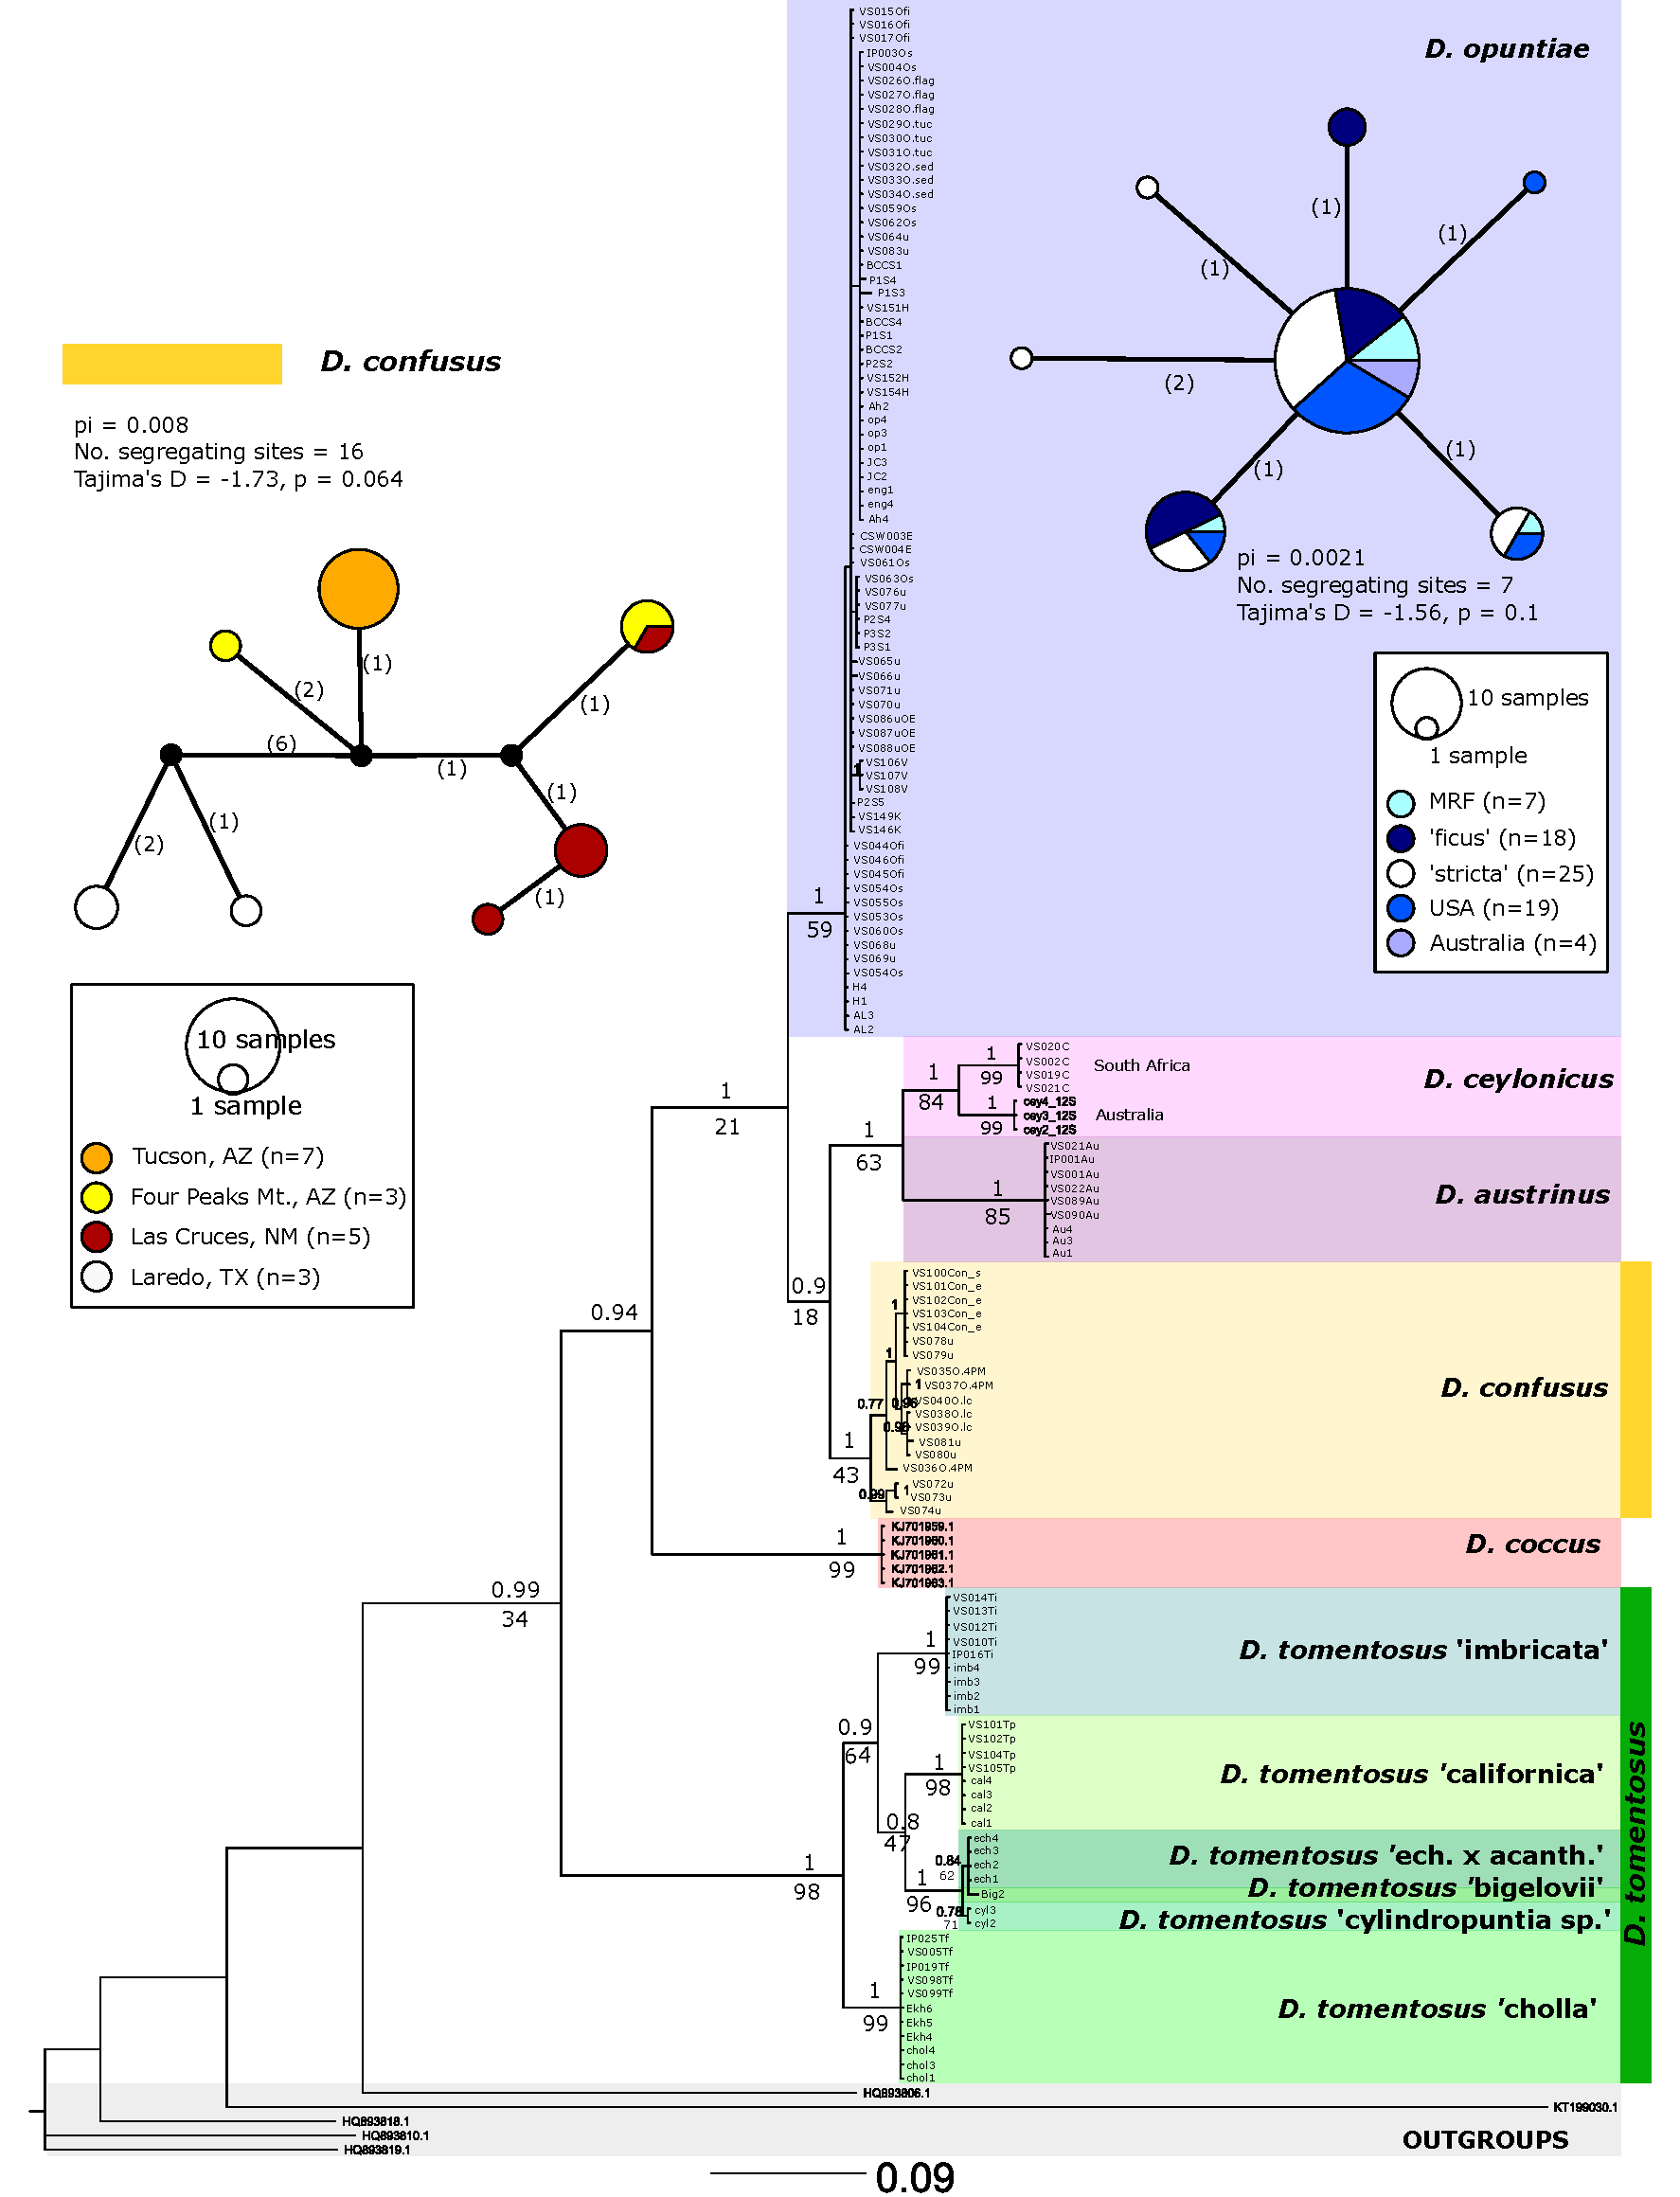
\includegraphics[scale =0.55]{Images/12S_MrBayes_2.pdf}
	\caption{Bayesian and Maximum likelihood phylogenies for the 12S gene region. Posterior probability values are above, and bootstrap values are below the branches. Haplotype networks are shown inset for \textit{D. opuntiae} and \textit{D. confusus}. Small black dots indicate missing haplotypes, and the diameter of each circle is proportional to the number of genetic sequences that comprise it. Numbers in brackets indicate the number of nucleotide differences between haplotypes.} 
	\label{fig:12S_tree}
\end{figure}

\clearpage
\begin{figure}[H]
	\centering
	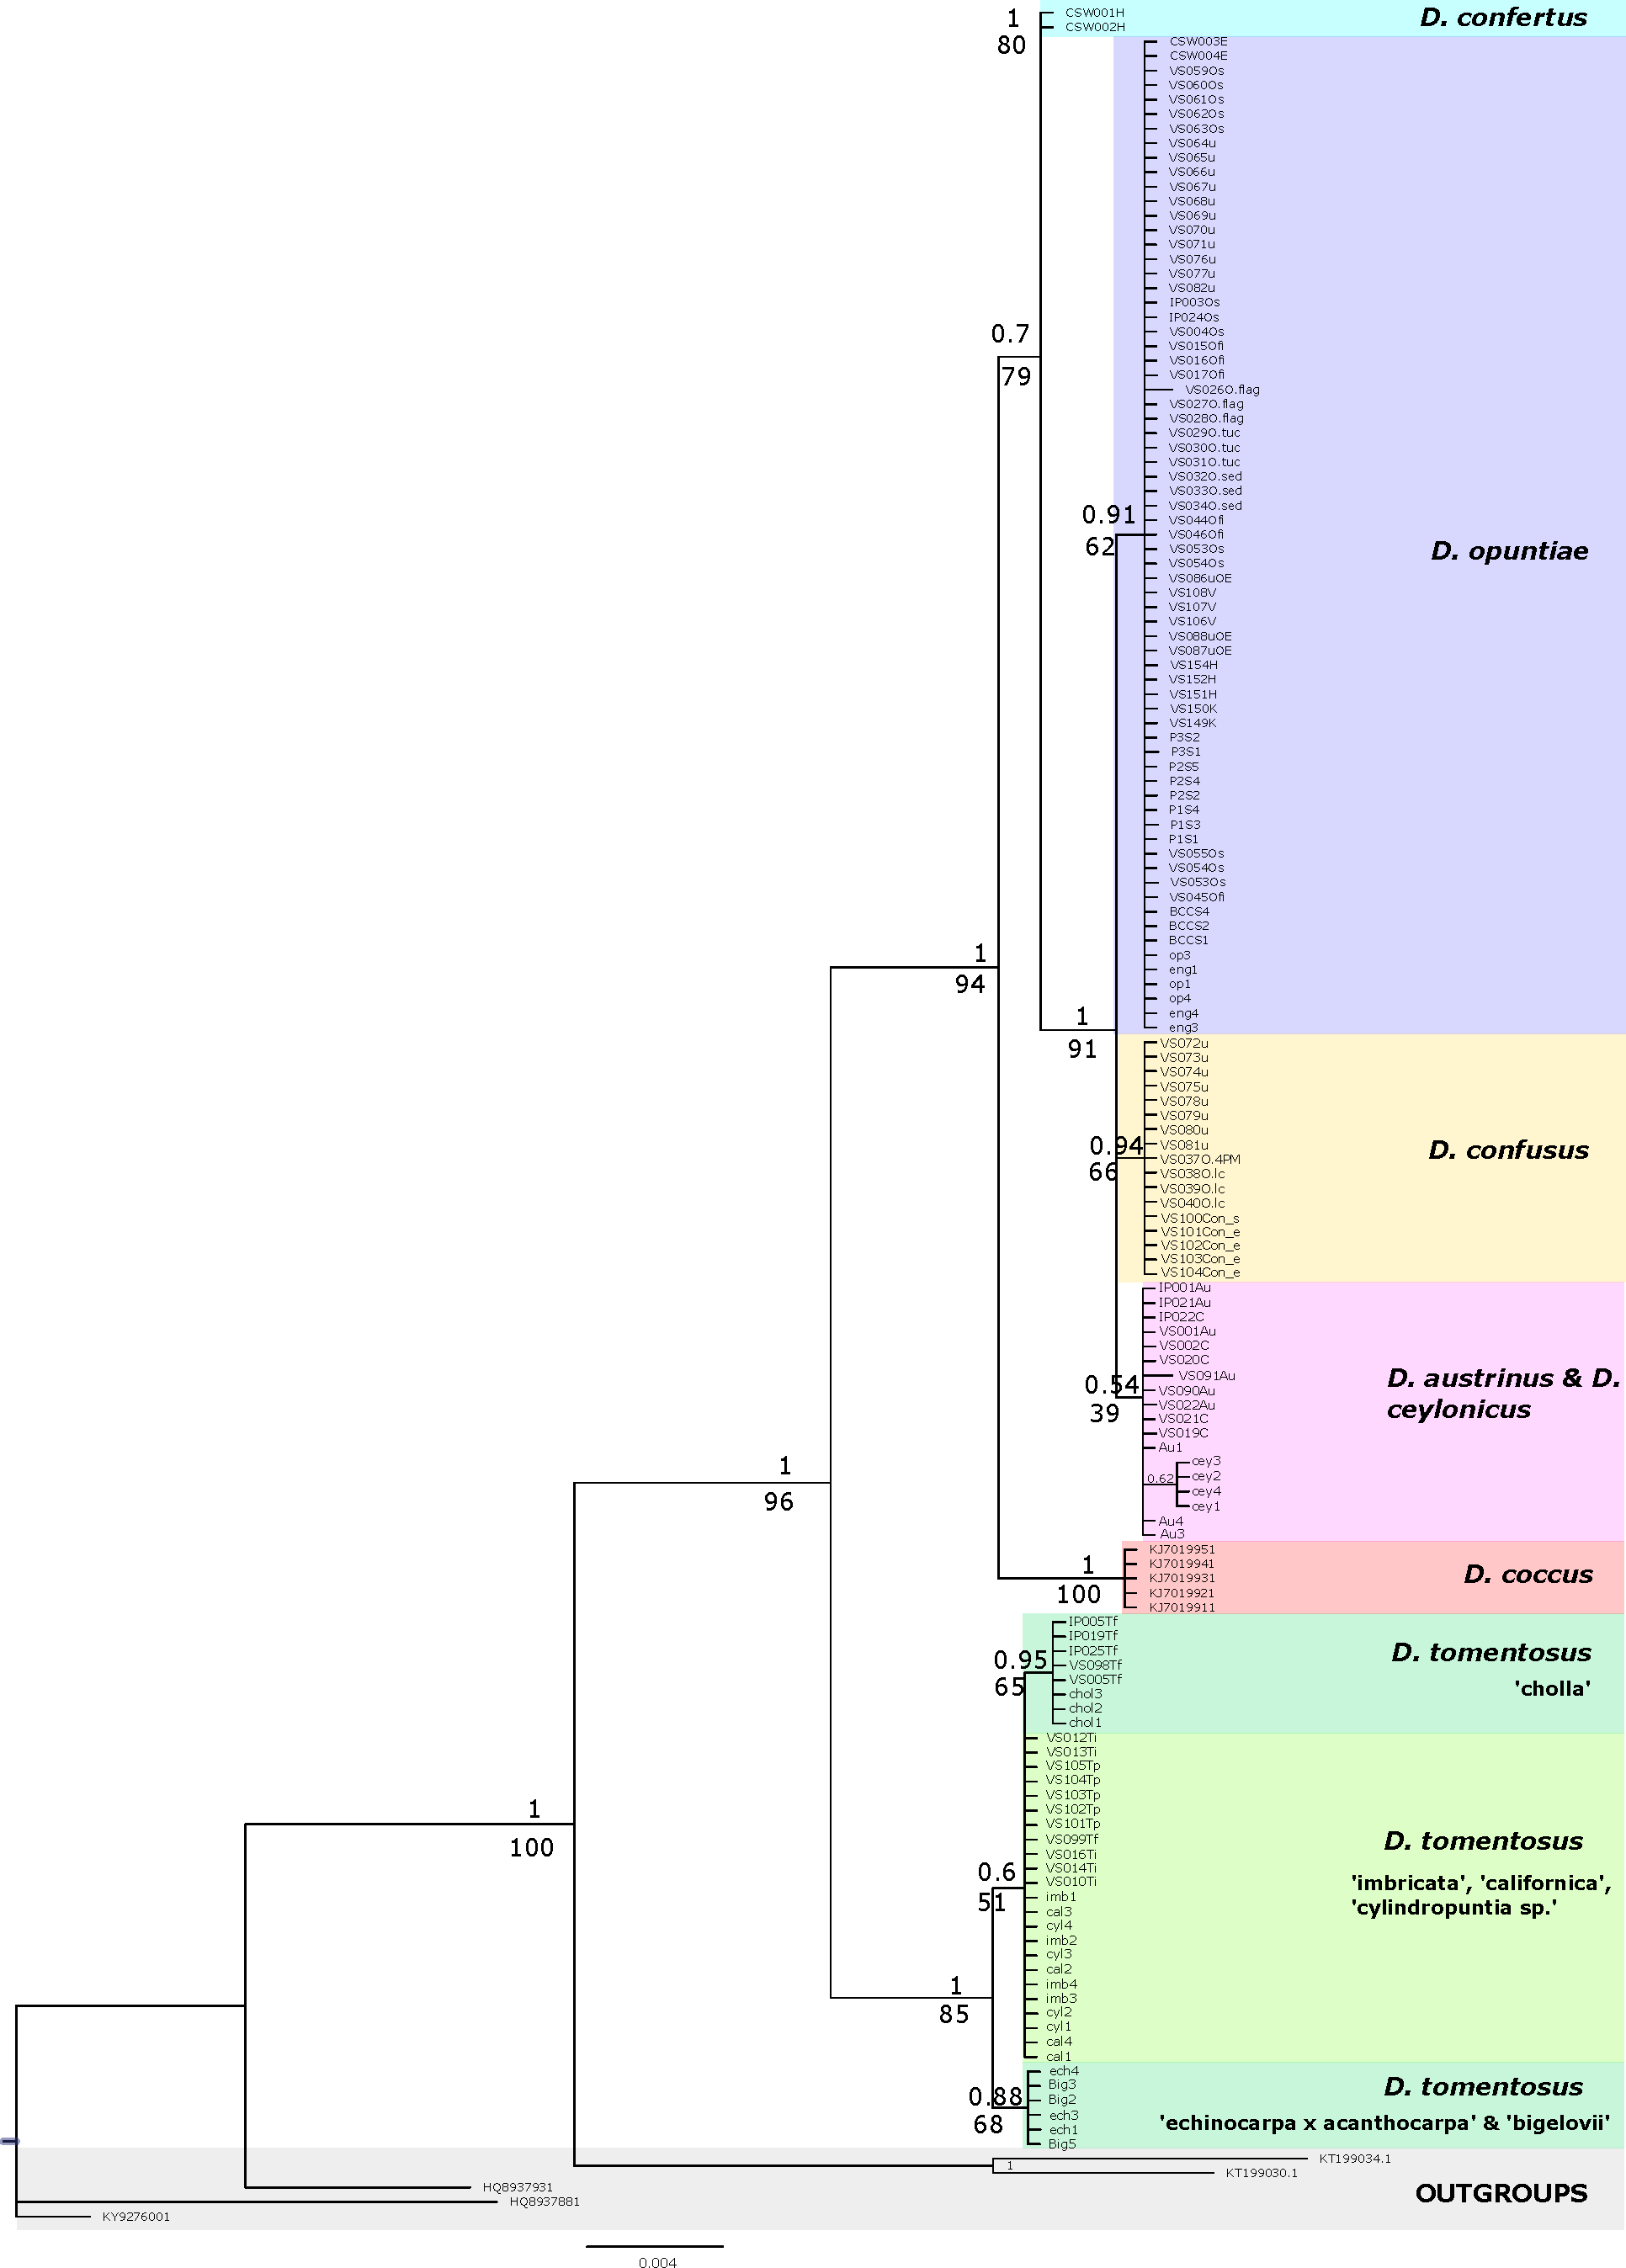
\includegraphics[scale =0.5]{Images/18S.pdf}
	\caption{Bayesian and Maximum likelihood  phylogenies for the 18S gene region. Posterior probability values are above, and bootstrap values are below the branches.} 
	\label{fig:18S_tree}
\end{figure}

\begin{figure}[H]
	\centering
	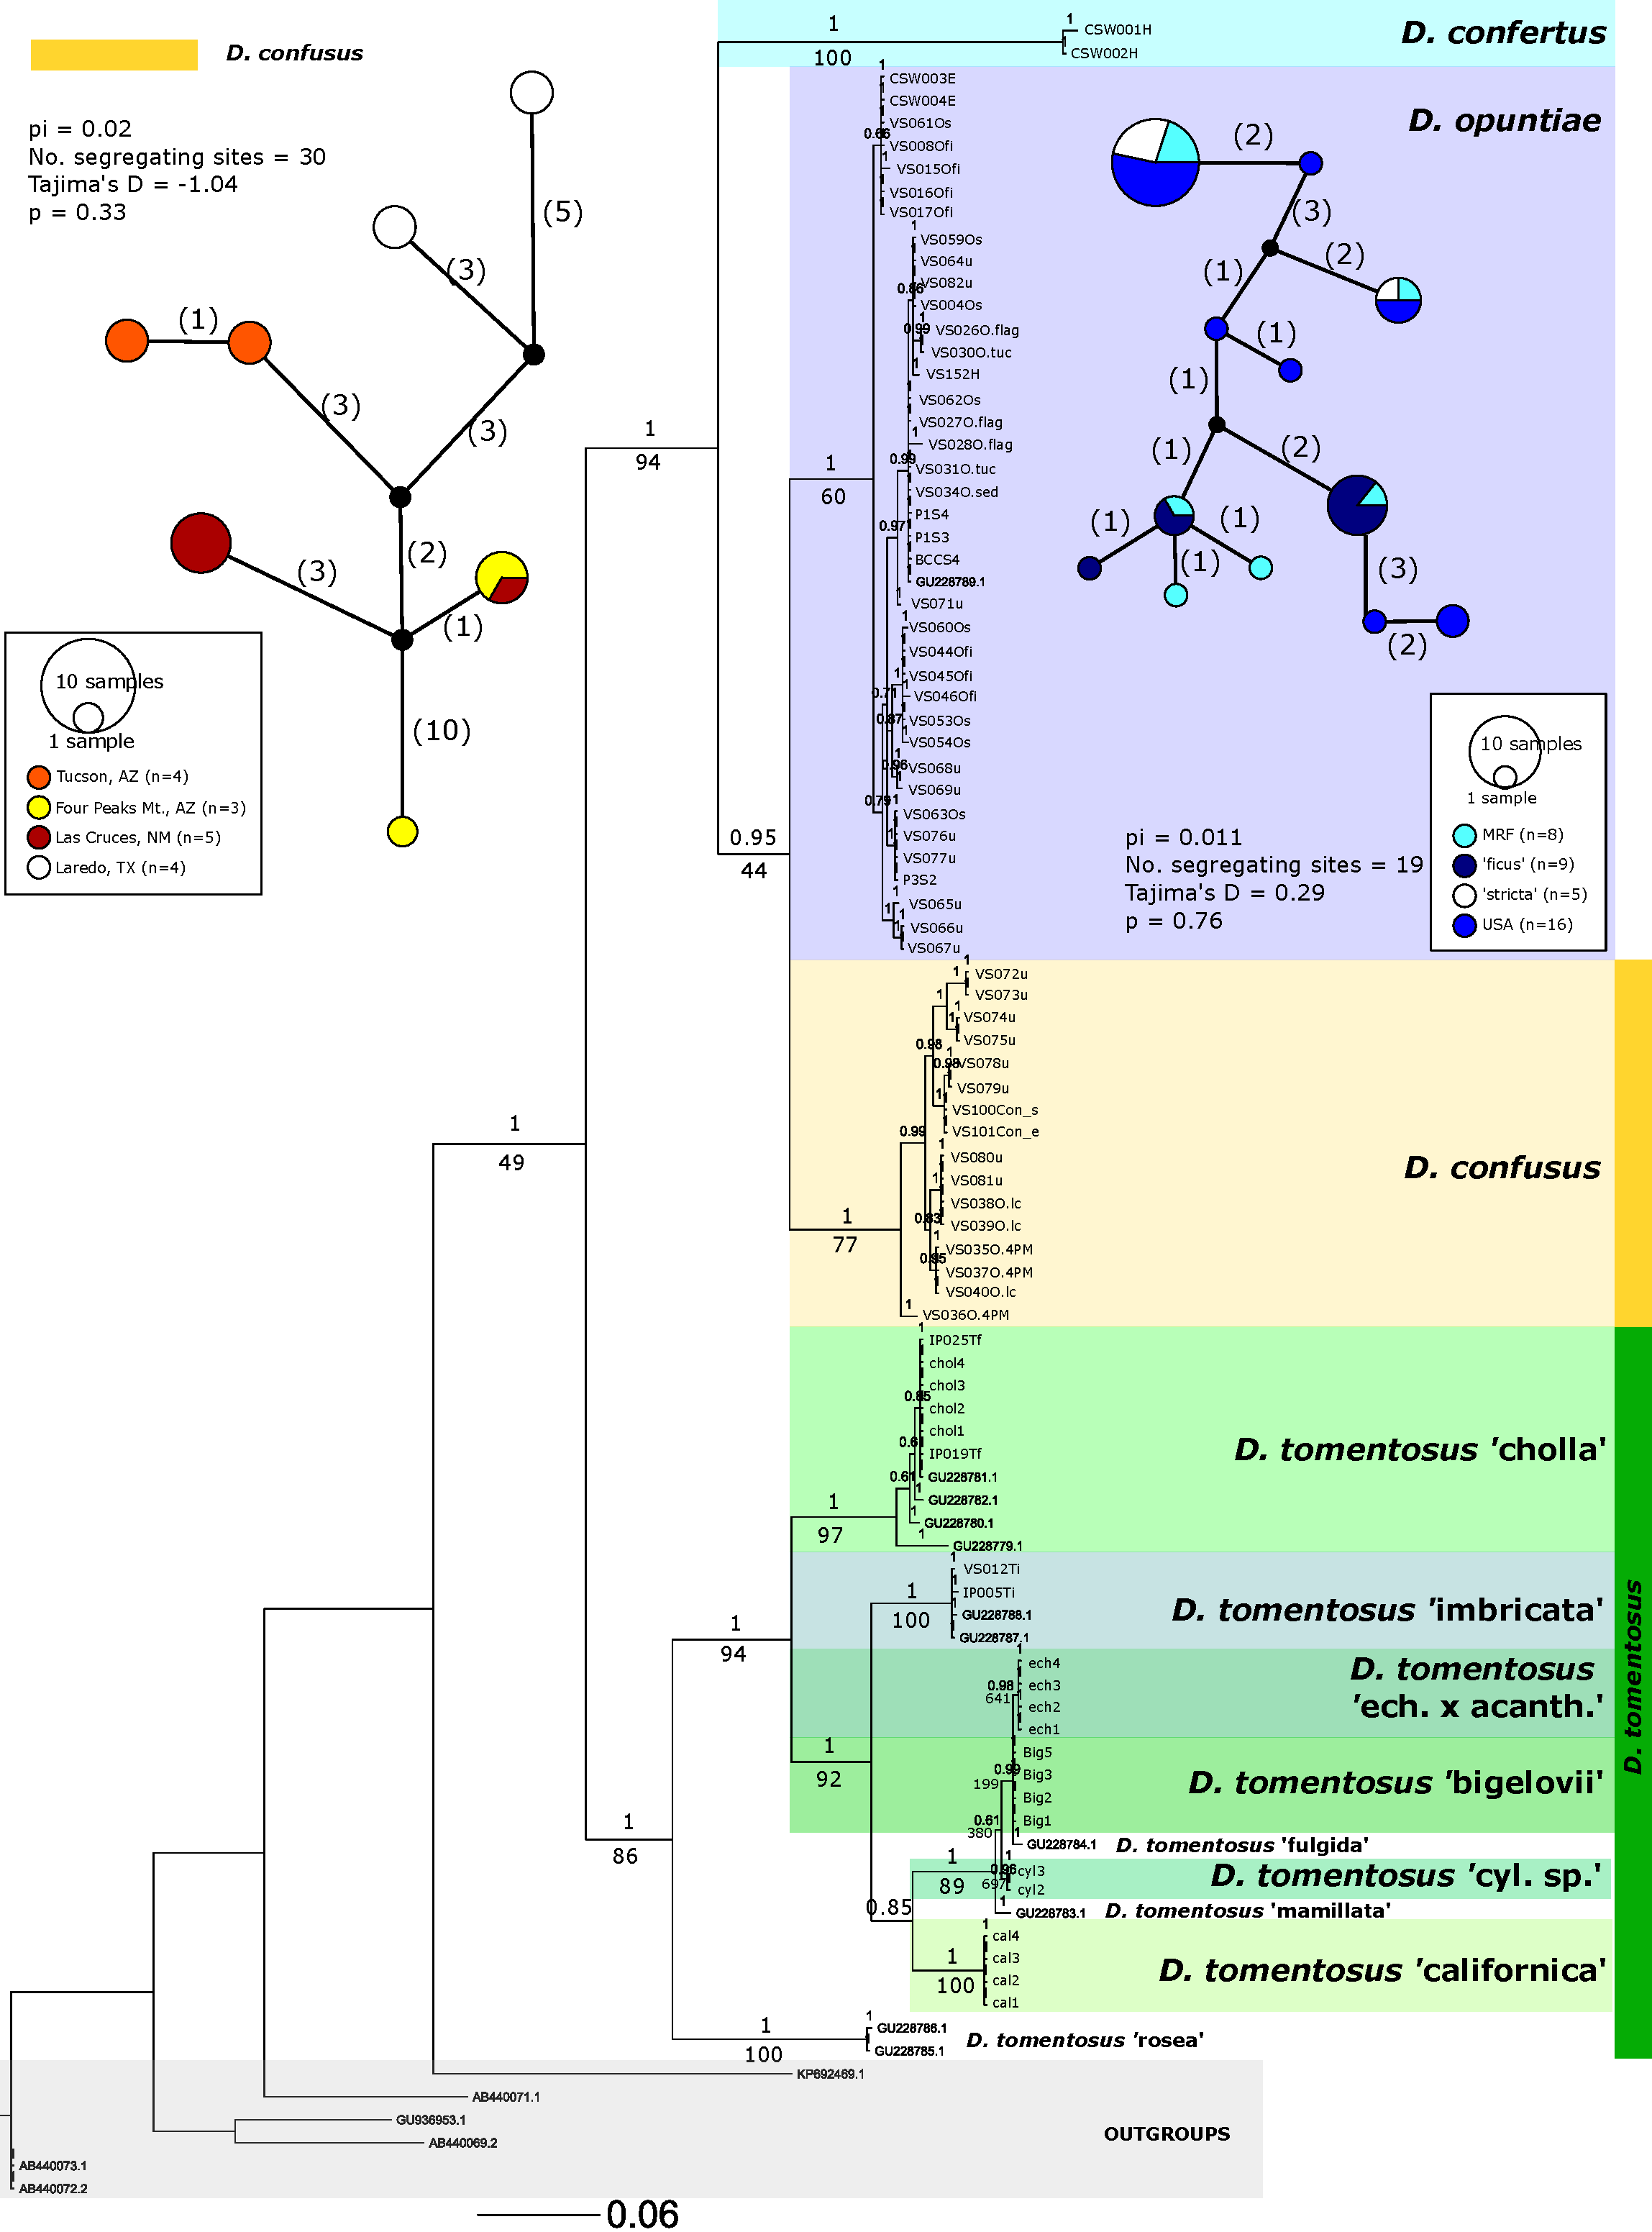
\includegraphics[scale =0.42]{Images/Bayesian_COI_both_primers.pdf}
	\caption{Bayesian and Maximum likelihood  phylogenies for the COI gene region. Posterior probabilities are above, and bootstrap values are below the branches. Haplotype networks are shown for \textit{D. opuntiae} and \textit{D. confusus}. Small black dots indicate missing haplotypes, and the diameter of each circle is proportional to the number of individuals it comprises. Numbers in brackets indicate the number of nucleotide differences between haplotypes.} 
	\label{fig:COI_tree}
\end{figure}

% \begin{landscape}

% \begin{figure}[H]
% 	\centering
% 	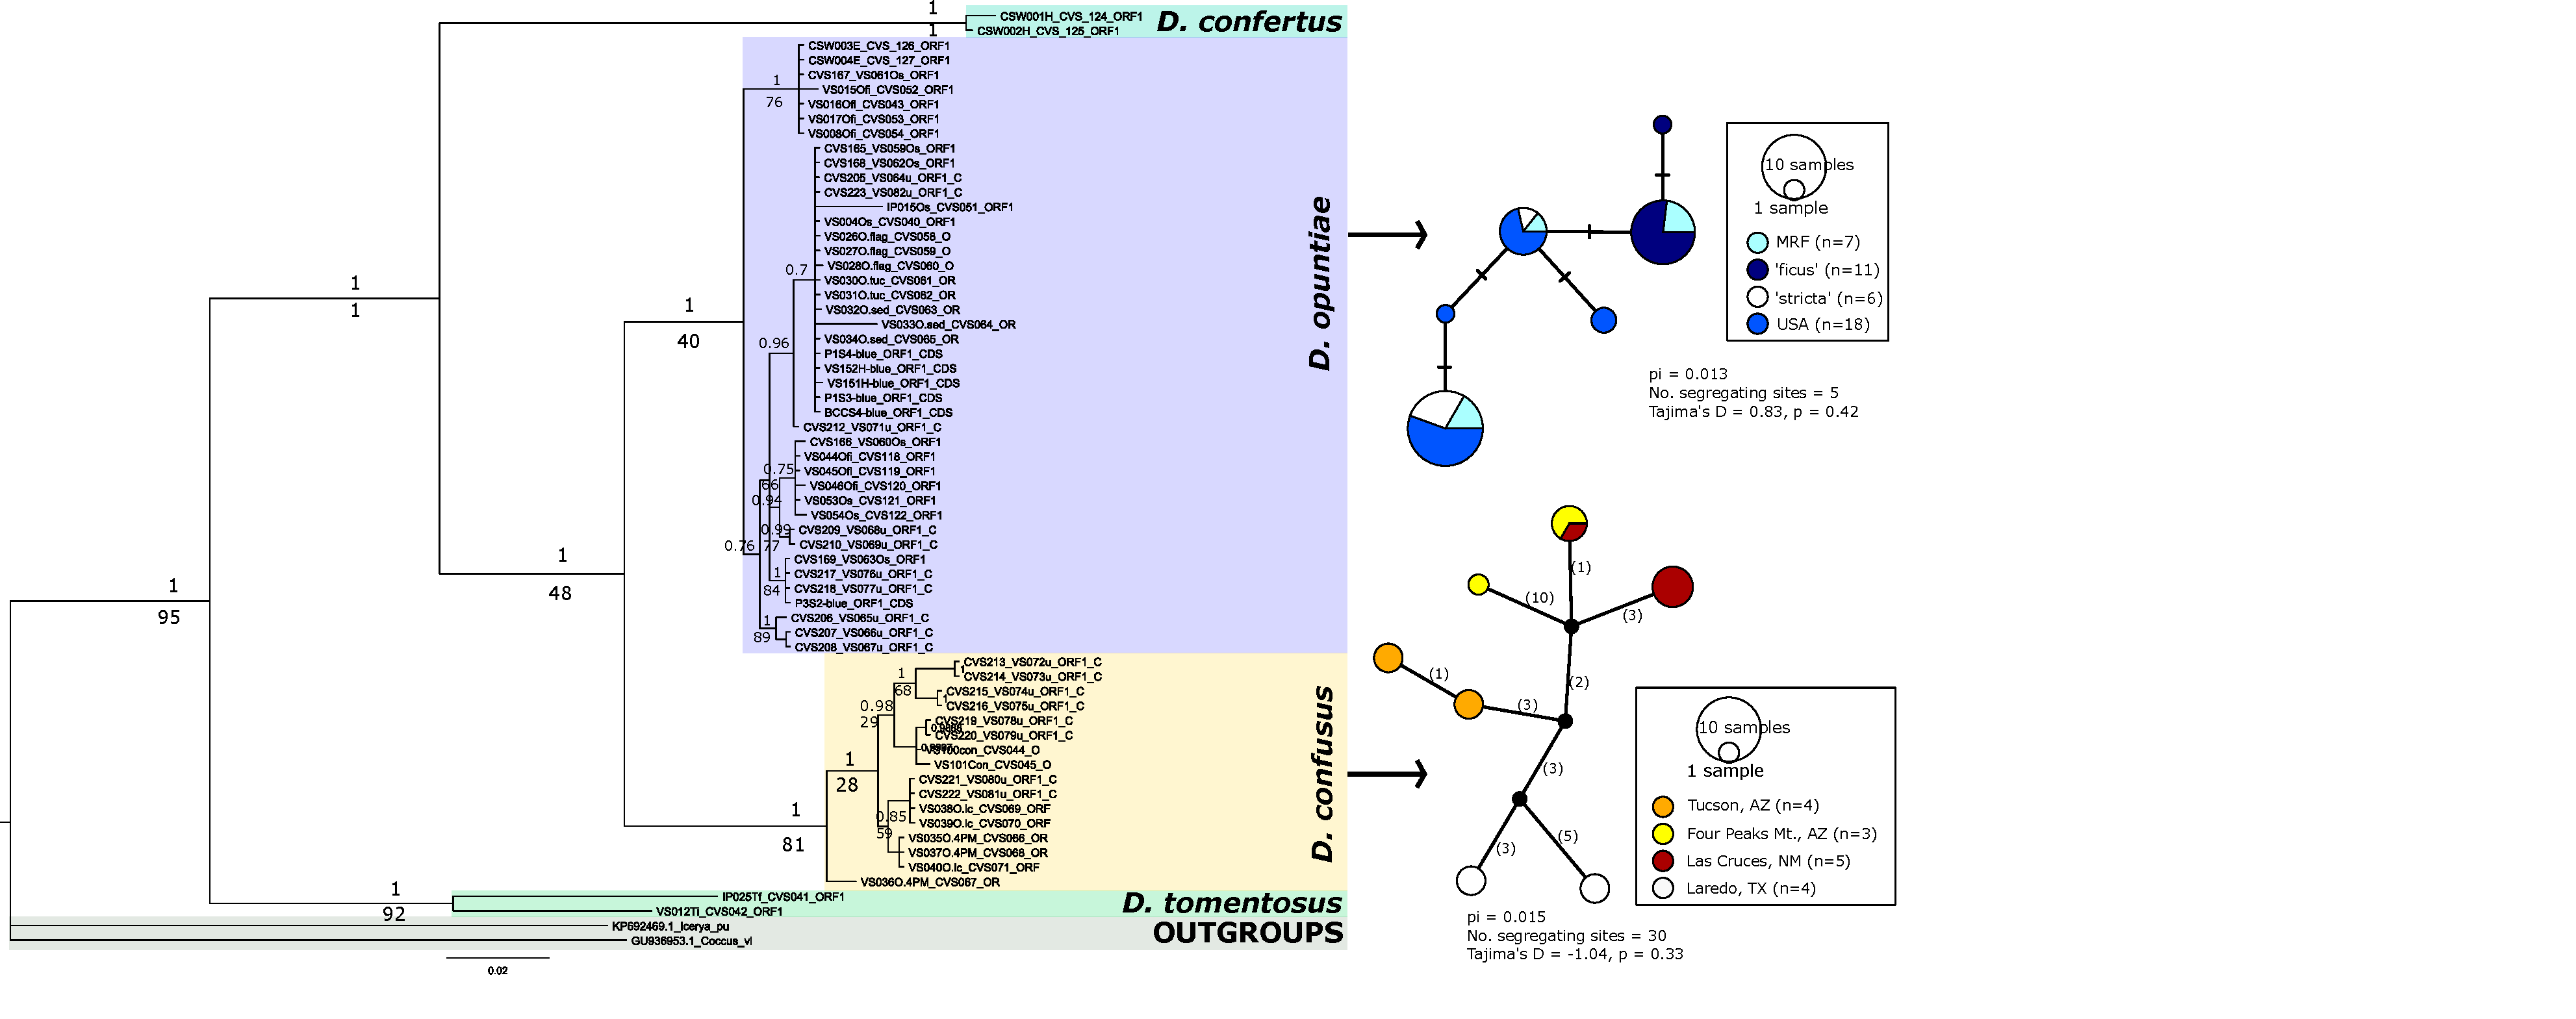
\includegraphics[scale =0.5]{Images/PCOF1.pdf}
% 	\caption{Bayesian (MrBayes) and Maximum likelihood (GARLI) phylogenetic trees for the COI (PCOF1 \& LepR1) gene. Bayesian posterior probability values are above, and Maximum likelihood bootstrap values are below the branches. Haplotype networks (using the TCS network method) are shown for \textit{D. opuntiae} and \textit{D. confusus}. Small black dots indicate missing haplotypes, and the diameter of each circle is proportional to the number of genetic sequences that share that particular haplotype. Hatch marks and numbers in brackets indicate the number of nucleotide differences between haplotypes.} 
% 	\label{fig:PCOF1_tree}
% \end{figure}

% \begin{figure}[H]
% \centering
% 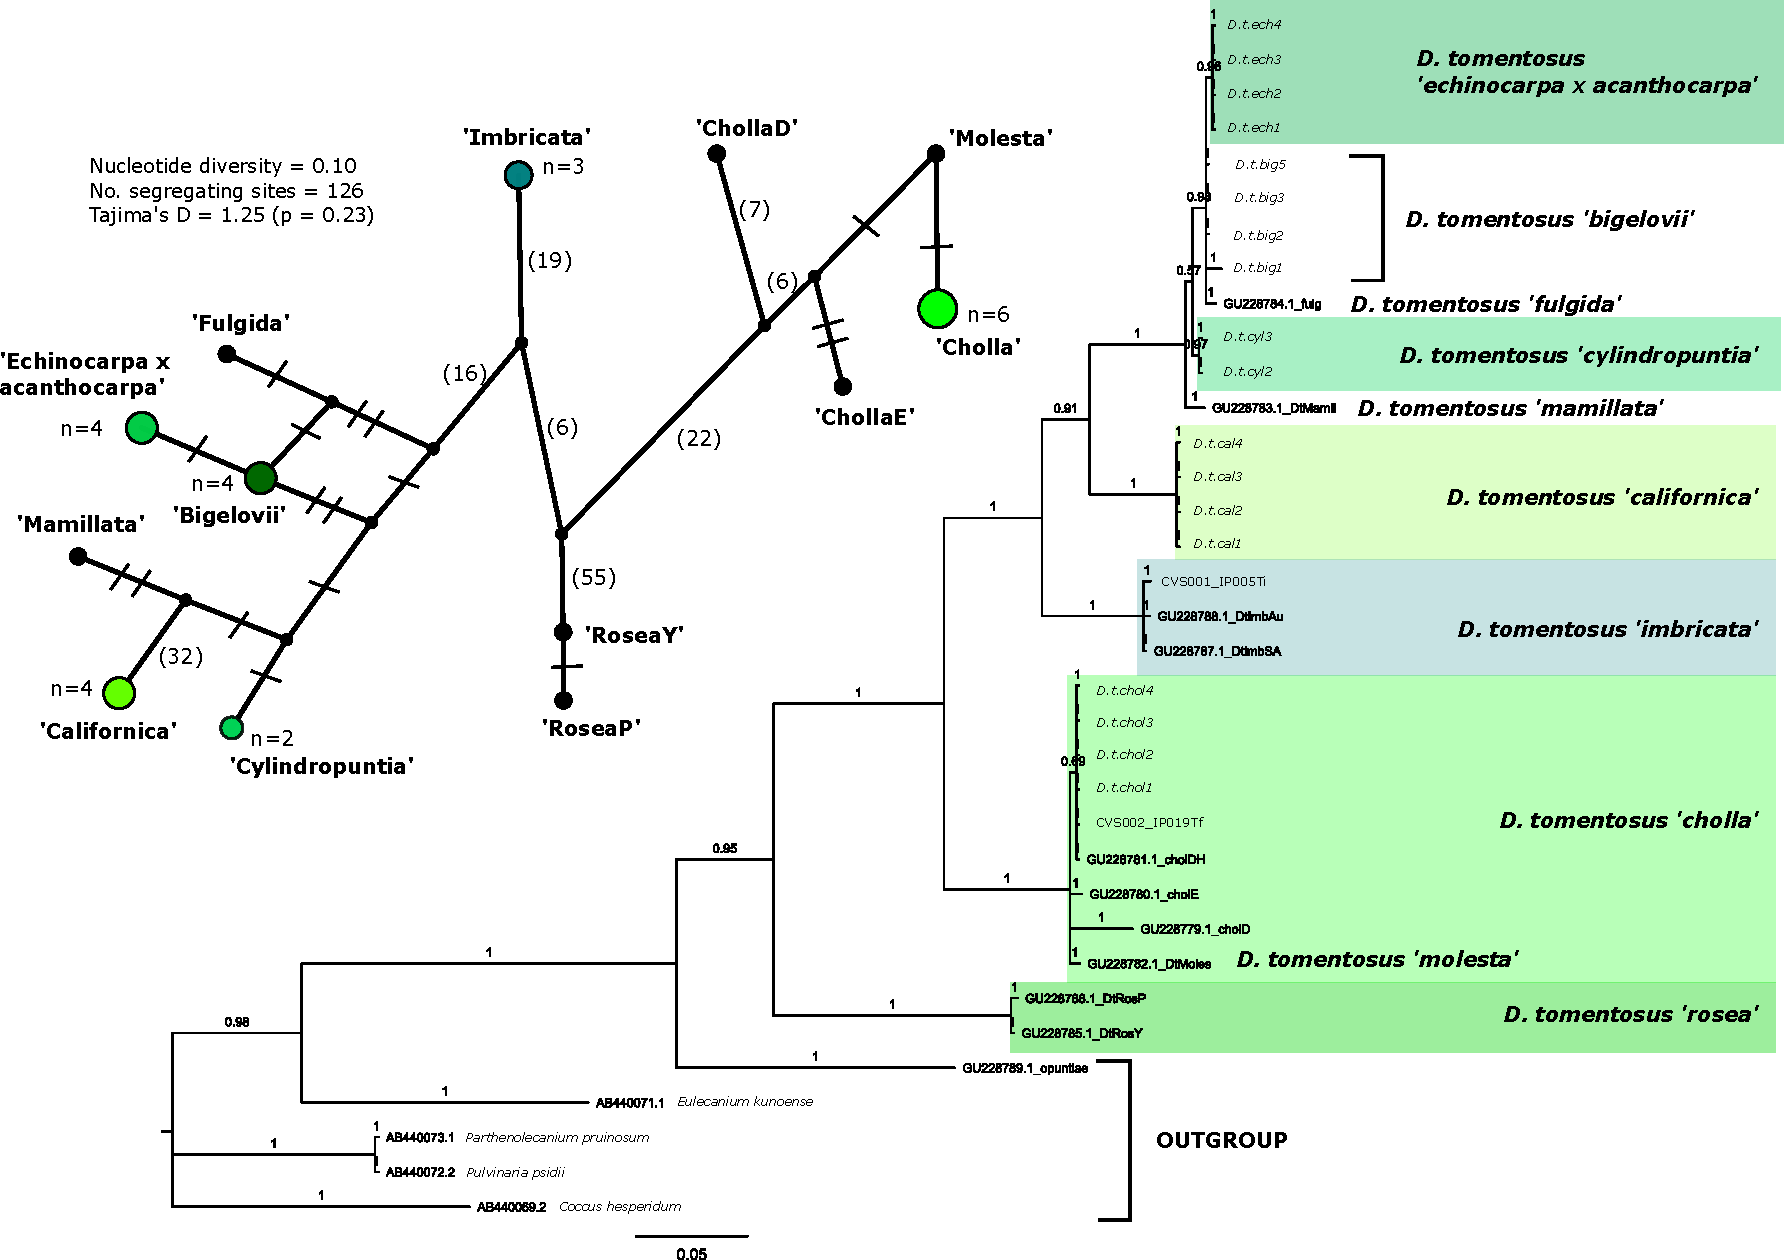
\includegraphics[scale = 0.75]{Images/COI_DTOM_BayesianTree.pdf}
% \caption{Bayesian phylogenetic tree for the COI(DTOMf \& HCO2198) gene. Posterior probabilities are shown on the branches. A haplotype network is shown alongside the tree (TCS network method) for \textit{D. tomentosus} lineages. Small black dots indicate missing haplotypes, and the diameter of each circle is proportional to the number of genetic sequences that share that particular haplotype. Hatch marks and numbers in brackets indicate the number of nucleotide differences between haplotypes.}
% \label{fig:COIDTOM_bayes}
% \end{figure}

% \begin{figure}[H]
% \centering
% 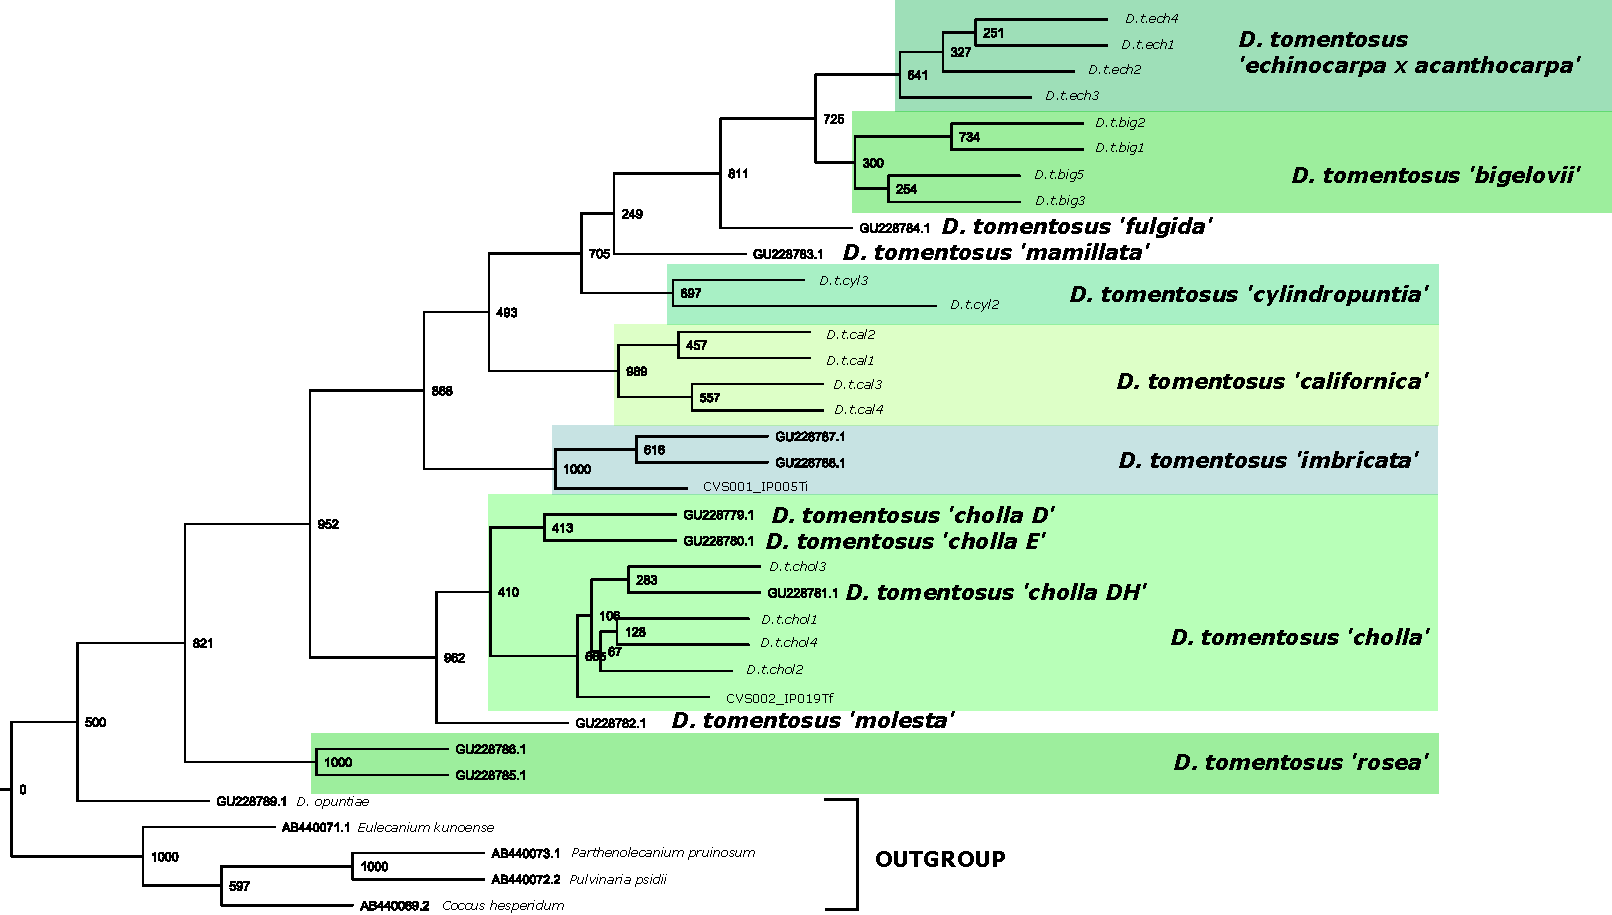
\includegraphics[scale = 0.85]{Images/COI_DTOM_GARLI.pdf}
% \caption{Maximum Likelihood phylogenetic tree for the COI(DTOMf \& HCO2198) gene. Bootstrap probabilities are shown on the branches.}
% \label{fig:COIDTOM_garli}
% \end{figure}

%  \end{landscape}

\begin{figure}[H]
	\centering
	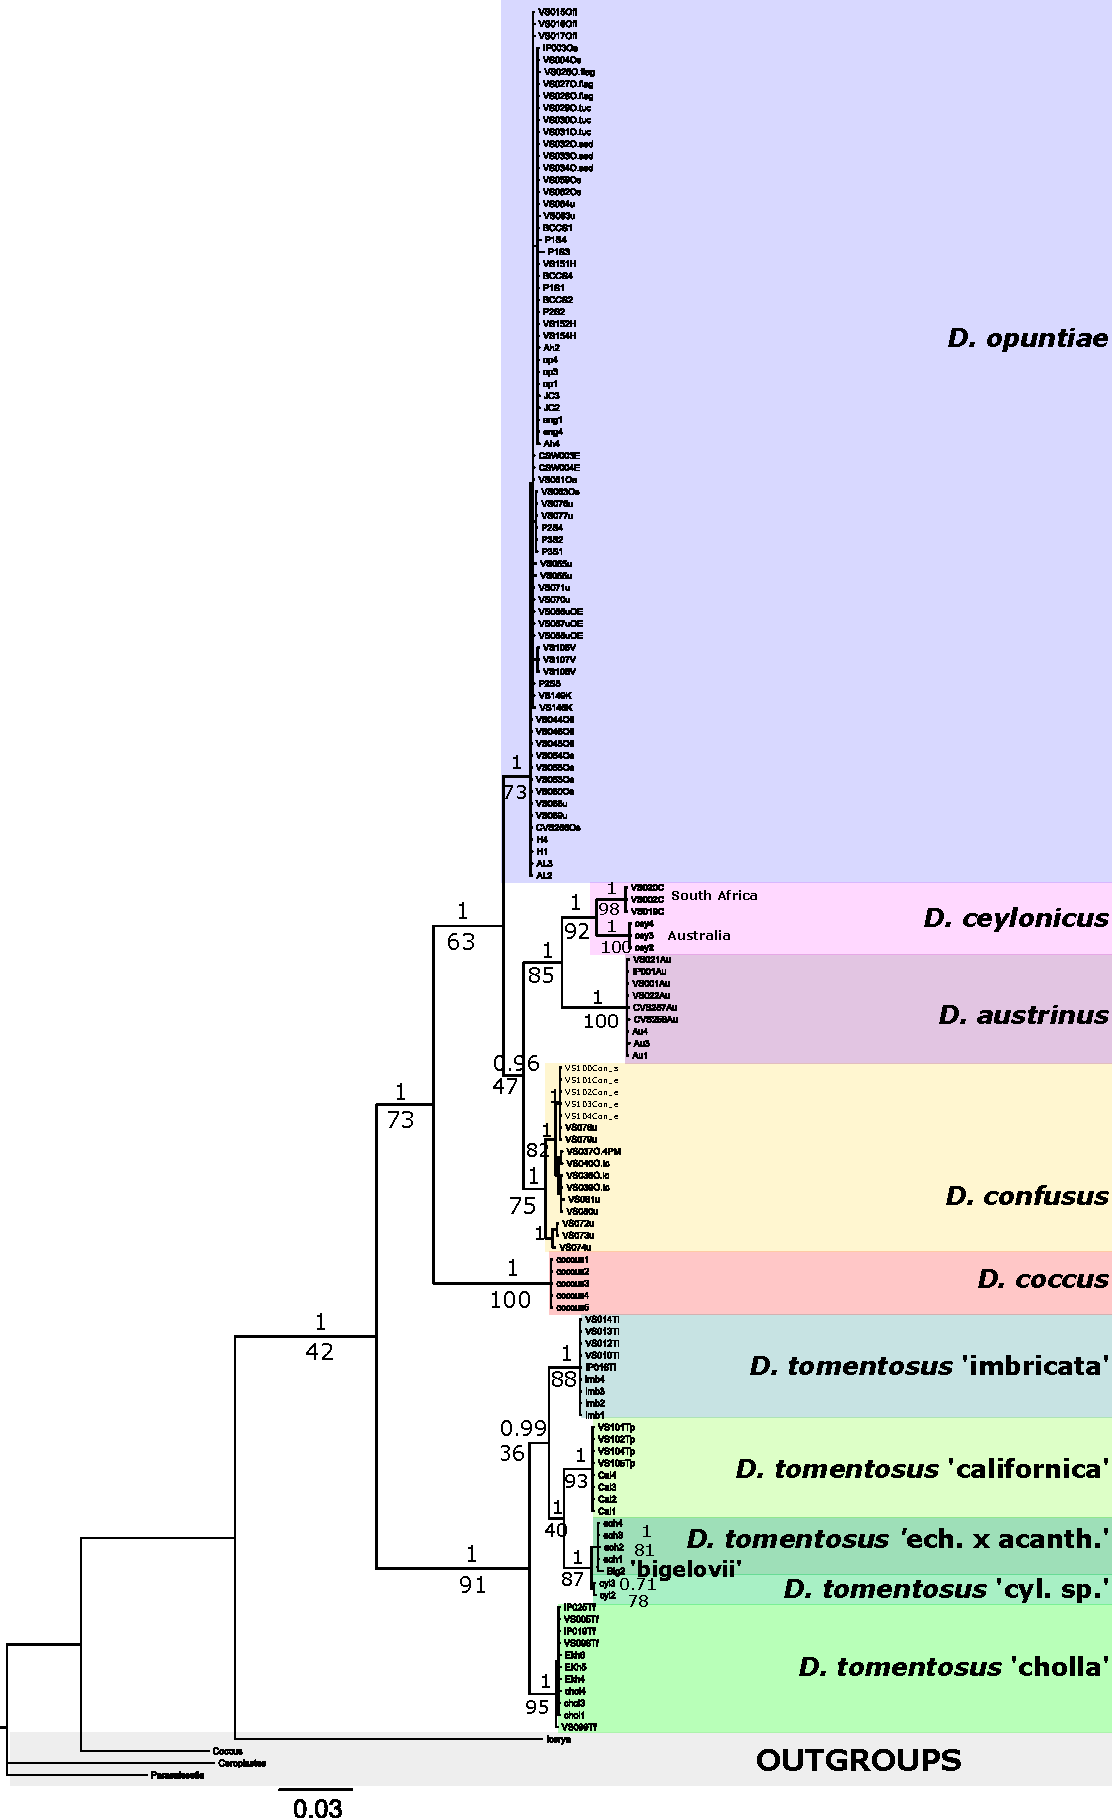
\includegraphics[scale =0.75]{Images/bayesian_concat2.pdf}
	\caption{Concatenated Bayesian and Maximum Likelihood phylogenies for the 12S and 18S gene regions. Bayesian posterior probability values are above, and Maximum likelihood bootstrap values are below the branches.} 
	\label{fig:concatTrees}
\end{figure}

\begin{landscape}
\begin{table}[H]
\renewcommand{\arraystretch}{0.4}
\caption{Within and between group p-distance matrix for the 12S gene, using the Kimura 2-parameter model. Species are represented by a total of 151 nucleotide sequences consisting of 779 positions. Bold values along the diagonal represent within-group p-distances.}
\label{tab:p_dist_12S}
\resizebox{\columnwidth}{!}{%
\begin{tabular}{@{}llllllllllll@{}}
\toprule
 & \textit{D. austrinus} & \textit{D. ceylonicus} & \textit{D. coccus} & \textit{D. confusus} & \textit{D. opuntiae} & \textit{D. tomentosus} `californica' & \textit{D. tomentosus} `cholla' & \textit{D. tomentosus} `cylindropuntia sp.' & \textit{D. tomentosus} `echinocarpa' & \textit{D. tomentosus} `imbricata' & Outgroup \\ \midrule
\begin{tabular}[l]{@{}l@{}} \textit{D. austrinus} \\ (n = 9) \end{tabular} & \textbf{0.000} &  &  &  &  &  &  &  &  &  &  \\
\begin{tabular}[l]{@{}l@{}} \textit{D. ceylonicus} \\ n = 6\end{tabular} & 0.17 & \textbf{0.050} &  &  &  &  &  &  &  &  &  \\
\begin{tabular}[l]{@{}l@{}} \textit{D. coccus} \\ n = 5\end{tabular} & 0.38 & 0.33 & \textbf{0.000} &  &  &  &  &  &  &  &  \\
\begin{tabular}[l]{@{}l@{}} \textit{D. confusus} \\ n = 18\end{tabular} & 0.17 & 0.16 & 0.30 & \textbf{0.015} &  &  &  &  &  &  &  \\
\begin{tabular}[l]{@{}l@{}} \textit{D. opuntiae} \\ n = 73\end{tabular} & 0.18 & 0.17 & 0.27 & 0.11 & \textbf{0.005} &  &  &  &  &  &  \\
\begin{tabular}[l]{@{}l@{}} \textit{D. tomentosus} `californica'\\ n = 8\end{tabular} & 0.42 & 0.39 & 0.41 & 0.39 & 0.42 & \textbf{0.000} &  &  &  &  &  \\
\begin{tabular}[l]{@{}l@{}} \textit{D. tomentosus} `cholla' \\ n = 12\end{tabular} & 0.39 & 0.38 & 0.39 & 0.37 & 0.39 & 0.13 & \textbf{0.068} &  &  &  &  \\
\begin{tabular}[l]{@{}l@{}} \textit{D. tomentosus} \\ `cylindropuntia sp.' \\ n = 2\end{tabular} & 0.42 & 0.41 & 0.41 & 0.40 & 0.40 & 0.09 & 0.14 & \textbf{0.000} &  &  &  \\
\begin{tabular}[l]{@{}l@{}} \textit{D. tomentosus} `echinocarpa' \\ n = 4\end{tabular} & 0.42 & 0.42 & 0.40 & 0.40 & 0.39 & 0.09 & 0.15 & 0.00 & \textbf{0.00} &  &  \\
\begin{tabular}[l]{@{}l@{}} \textit{D. tomentosus} `imbricata' \\ n = 9\end{tabular} & 0.44 & 0.40 & 0.40 & 0.41 & 0.42 & 0.10 & 0.13 & 0.09 & 0.09 & \textbf{0.00} &  \\
\begin{tabular}[l]{@{}l@{}} Outgroup \\ n = 5\end{tabular} & 0.70 & 0.66 & 0.71 & 0.65 & 0.67 & 0.73 & 0.75 & 0.73 & 0.71 & 0.74 & \textbf{0.903} \\ \bottomrule
\end{tabular}
}
\end{table}

\begin{table}[H]
\renewcommand{\arraystretch}{0.5}
\caption{Within and between group p-distance matrix for the 18S gene, using the Kimura 2-parameter model. Species are represented by a total of 153 nucleotide sequences consisting of 630 positions. Bold values along the diagonal represent within-group p-distances.}
\label{tab:p_dist_18S}
\resizebox{\columnwidth}{!}{%
\begin{tabular}{@{}lp{3.8cm}llllllll@{}}
\toprule
 & \begin{tabular}[c]{@{}l@{}} \textit{D. austrinus} \&\\ \textit{D. ceylonicus}  \end{tabular} & \textit{D. coccus} & \textit{D. confertus} & \textit{D. confusus} & \textit{D. opuntiae} & \textit{D. tomentosus} & \begin{tabular}[c]{@{}l@{}} \textit{D. tomentosus} `echinocarpa'\\ \& \textit{D. tomentosus} `bigelovii' \end{tabular} & \textit{D. tomentosus} `cholla' & Outgroup \\ \midrule
\begin{tabular}[c]{@{}l@{}} \textit{D. austrinus} \&\\ \textit{D. ceylonicus} (n=18) \end{tabular}  & \textbf{0.006} &  &  &  &  &  &  &  &  \\
\textit{D. coccus} (n=5)  & 0.033 & \textbf{0} &  &  &  &  &  &  &  \\
\textit{D. confertus} (n=2) & 0.016 & 0.020 & \textbf{0} &  &  &  &  &  &  \\
\textit{D. confusus} (n=17)  & 0.010 & 0.027 & 0.012 & \textbf{0} &  &  &  &  &  \\
\textit{D. opuntiae} (n=69)  & 0.010 & 0.028 & 0.013 & 0.004 & \textbf{0} &  &  &  &  \\
\textit{D. tomentosus} (n=31)  & 0.057 & 0.048 & 0.043 & 0.047 & 0.049 & \textbf{0} &  &  &  \\
\begin{tabular}[c]{@{}l@{}} \textit{D. tomentosus} `echinocarpa'\\ \& \textit{D. tomentosus} `bigelovii' (n=6) \end{tabular}  & 0.058 & 0.049 & 0.043 & 0.047 & 0.050 & 0.004 & \textbf{0} &  &  \\
\textit{D. tomentosus} `cholla' (n=5)  & 0.059 & 0.047 & 0.045 & 0.049 & 0.051 & 0.002 & 0.005 & \textbf{0} &  \\
Outgroup (n=5) & 0.134 & 0.129 & 0.123 & 0.125 & 0.127 & 0.114 & 0.117 & 0.116 & \textbf{0.114} \\ \bottomrule
\end{tabular}
}
\end{table}
\end{landscape}

\begin{landscape}

\begin{table}[]
\renewcommand{\arraystretch}{0.5}
\caption{Within and between group p-distance matrix for the COI-A and COI-B regions, using the Kimura 2-parameter model. Species are represented by a total of 95 nucleotide sequences consisting of 603 positions. Bold values along the diagonal represent within-group p-distances.}
\label{tab:p_dist_COI}
\centering
 \resizebox{\columnwidth}{!}{%
\begin{tabular}{@{}llllllllllll@{}}
\toprule
 & \textit{D. confusus} & \textit{D. confertus} & \textit{D. opuntiae} & \begin{tabular}[c]{@{}l@{}} \textit{D. tomentosus} \\ `bigelovii'\end{tabular} & \begin{tabular}[c]{@{}l@{}} \textit{D. tomentosus} \\ `californica'\end{tabular} & \begin{tabular}[c]{@{}l@{}} \textit{D. tomentosus} \\ `cholla'\end{tabular} & \begin{tabular}[c]{@{}l@{}} \textit{D. tomentosus} \\ `cylindropuntia sp.'\end{tabular} & \begin{tabular}[c]{@{}l@{}} \textit{D. tomentosus} \\ `echinocarpa'\end{tabular} & \begin{tabular}[c]{@{}l@{}} \textit{D. tomentosus} \\ `imbricata'\end{tabular} & \begin{tabular}[c]{@{}l@{}} \textit{D. tomentosus} \\ 'rosea'\end{tabular} & Outgroups \\ \midrule
\textit{D. confusus} (n=16) & \textbf{0.017} &  &  &  &  &  &  &  &  &  &  \\
\textit{D. confertus} (n=2) & 0.29 & \textbf{0.008} &  &  &  &  &  &  &  &  &  \\
\textit{D. opuntiae} (n=39) & 0.13 & 0.28 & \textbf{0.014} &  &  &  &  &  &  &  &  \\
\textit{D. tomentosus} `bigelovii' (n=4) & 0.24 & 0.36 & 0.23 & \textbf{0.000} &  &  &  &  &  &  &  \\
\textit{D. tomentosus} `californica' (n=4) & 0.24 & 0.31 & 0.24 & 0.09 & \textbf{0.000} &  &  &  &  &  &  \\
\textit{D. tomentosus} `cholla' (n=9) & 0.27 & 0.36 & 0.25 & 0.14 & 0.14 & \textbf{0.009} &  &  &  &  &  \\
\textit{D. tomentosus} `cylindropuntia sp.' (n=2) & 0.24 & 0.36 & 0.24 & 0.01 & 0.09 & 0.15 & \textbf{0.000} &  &  &  &  \\
\textit{D. tomentosus} `echinocarpa' (n=4) & 0.25 & 0.37 & 0.23 & 0.00 & 0.10 & 0.15 & 0.01 & \textbf{0.000} &  &  &  \\
\textit{D. tomentosus} `imbricata' (n=4) & 0.26 & 0.34 & 0.23 & 0.10 & 0.11 & 0.14 & 0.10 & 0.10 & \textbf{0.002} &  &  \\
\textit{D. tomentosus} `rosea' (n=2) & 0.25 & 0.31 & 0.25 & 0.22 & 0.23 & 0.21 & 0.23 & 0.22 & 0.21 & \textbf{0.002} &  \\
Outgroups & 0.34 & 0.44 & 0.32 & 0.34 & 0.33 & 0.32 & 0.34 & 0.34 & 0.32 & 0.31 & \textbf{0.235} \\ \bottomrule
\end{tabular}
}
\end{table}


% \begin{table}[H]
% \renewcommand{\arraystretch}{0.5}
% \caption{Within and between group p-distance matrix for the COI (DTOMf \& HCO2198) gene, using the Kimura 2-paramter model. Species are represented by a total of 32 nucleotide sequences consisting of 546 positions. Bold values along the diagonal represent within group p-distances.}
% \label{tab:p_dist_dtom}
% \resizebox{\columnwidth}{!}{%
% \begin{tabular}{@{}lllllllll@{}}
% \toprule
%  & \textit{\begin{tabular}[c]{@{}l@{}}D. tomentosus 'echinocarpa x \\ acanthocarpa'\end{tabular}} & \textit{\begin{tabular}[c]{@{}l@{}}D. tomentosus \\ 'cylindropuntia'\end{tabular}} & \textit{\begin{tabular}[c]{@{}l@{}}D. tomentosus \\ 'cholla'\end{tabular}} & \textit{\begin{tabular}[c]{@{}l@{}}D. tomentosus \\ 'californica'\end{tabular}} & \textit{\begin{tabular}[c]{@{}l@{}}D. tomentosus \\ 'bigelovii'\end{tabular}} & \textit{\begin{tabular}[c]{@{}l@{}}D. tomentosus \\ 'imbricata'\end{tabular}} & \textit{\begin{tabular}[c]{@{}l@{}}D. tomentosus \\ 'rosea'\end{tabular}} & Outgroup \\ \midrule
% \textit{\begin{tabular}[c]{@{}l@{}}D. tomentosus 'echinocarpa x \\ acanthocarpa' (n=4)\end{tabular}} & \textbf{0} &  &  &  &  &  &  &  \\
% \textit{\begin{tabular}[c]{@{}l@{}}D. tomentosus \\ 'cylindropuntia' (n=2)\end{tabular}} & 0.011 & \textbf{0} &  &  &  &  &  &  \\
% \textit{\begin{tabular}[c]{@{}l@{}}D. tomentosus \\ 'cholla' (n=8)\end{tabular}} & 0.146 & 0.152 & \textbf{0.1} &  &  &  &  &  \\
% \textit{\begin{tabular}[c]{@{}l@{}}D. tomentosus \\ 'californica' (n=4)\end{tabular}} & 0.096 & 0.089 & 0.139 & \textbf{0} &  &  &  &  \\
% \textit{\begin{tabular}[c]{@{}l@{}}D. tomentosus \\ 'bigelovii' (n=4)\end{tabular}} & 0.004 & 0.010 & 0.145 & 0.094 & \textbf{0.003} &  &  &  \\
% \textit{\begin{tabular}[c]{@{}l@{}}D. tomentosus \\ 'imbricata' (n=3)\end{tabular}} & 0.102 & 0.102 & 0.143 & 0.105 & 0.100 & \textbf{0.003} &  &  \\
% \textit{\begin{tabular}[c]{@{}l@{}}D. tomentosus \\ 'rosea' (n=2)\end{tabular}} & 0.218 & 0.226 & 0.213 & 0.222 & 0.216 & 0.212 & \textbf{0.002} &  \\
% \begin{tabular}[c]{@{}l@{}}Outgroup \\ (n=5)\end{tabular} & 0.317 & 0.313 & 0.298 & 0.312 & 0.314 & 0.296 & 0.288 & \textbf{0.23} \\ \bottomrule
% \end{tabular}
% }
% \end{table}

\end{landscape}

\section{Identification accuracy}

\subsection{Nearest Neighbour (NN) results}
For species-level identification at a default distance threshold of 1\%, the NN algorithm can be a useful test of accuracy. However, when different genes are being analysed that display different evolutionary rates, an adjustable threshold value is required. The NN algorithm tends to result in an abnormally high number of false positive identifications, and is therefore not considered further. For example, Table \ref{tab:barcode_test_results} shows a NN `True' outcome of 88.46\% for the correct identification of the \textit{D. opuntiae} lineages using the COI region, while the more stringent TID test only had an accuracy rate of 59.62\% at a lower threshold of 0.8\%.  

\subsection{12S}
At the species level, and at the optimal genetic distance threshold of 1\%, identification accuracy (IA) was 100\% for both barcode tests (BCM and TID) (Table \ref{tab:barcode_test_results}). At the lineage level, \textit{Dactylopius tomentosus} had an IA of 100\% (BCM) and 82.4\% (TID) at a distance threshold of 1\%. The TID result increased to 100\% at a lower optimal threshold value of 0.2\%. \textit{Dactylopius opuntiae} only had an IA of 15.22\% (with ambiguities at 82.61\% and incorrect IDs at 2.17\%) for the BCM test and a zero IA (100\% ambiguities) for the TID test at a threshold of 1\%. At a decreased threshold of 0.2\%, the TID only increased to a 13.04\% IA, with amibiguities at 80.43\% (incorrect and no IDs at 2.17\% and 4.35\%, respectively). The range of threshold genetic distance values for the \textit{D. opuntiae} lineages all showed a high occurrence of false negatives. 
Barcode gaps at the species level and for \textit{D. tomentosus} lineages were all positive (i.e., interspecific $>$ intraspecific variation), while the lineages within \textit{D. opuntiae} were all negative (i.e., interspecific $<$ intraspecific variation). Of the \textit{D. tomentosus} lineages, the `cylindropuntia sp.' and `echinocarpa x acanthocarpa' lineages had the smallest barcode gaps. 

\subsection{18S}
At the species level, and at the default genetic threshold of 1\%, IA was 94.59\% (5.41\% ambiguity) for the BCM test, but only 29.73\% (70.27\% ambiguities) for the TID test (Table \ref{tab:barcode_test_results}). At a lower threshold of 0.2\%, the IA for both the BCM and TID tests were 94.59\%, with ambiguities of 5.41\%. At the lineage level, at a threshold of 0.1\%, \textit{D. tomentosus} had an IA of 22.22\% (77.78\% ambiguities) for both the BCM and TID tests. The intraspecific lineages of \textit{Dactylopius opuntiae} produced 100\% ambiguous results for the BCM and TID tests at the 0.1\% threshold. The range of genetic threshold distance values for the lineages within \textit{D. tomentosus} and \textit{D. opuntiae} all showed a high number of false negatives. 
Barcode gaps at the species level were all positive, except for \textit{D. austrinus} and \textit{D. ceylonicus} sequences, which had negative barcode gaps (as illustrated in the phylogenetic tree in Figure \ref{fig:18S_tree}). The largest positive barcode gaps at the species level were for \textit{D. tomentosus}. Barcode gaps for \textit{D. opuntiae} and \textit{D. tomentosus} at the lineage level were all zero (i.e., the intra-and interspecific variation in these groups were equal); except for \textit{D. tomentosus} `cholla' sequences, which had positive barcode gaps. 

\subsection{COI}
Identification accuracy at the species level at a 1\% threshold was 100\% for both the BCM and TID tests (Table \ref{tab:barcode_test_results}). At the lineage level, at a 1\% threshold, \textit{D. opuntiae} had an IA of 61.54\% (32.69\% ambiguities and 5.77\% incorrect) for the BCM test, and an IA of 46.15\% (51.92\% ambiguities and 1.92\% incorrect) for the TID test. The BCM test results remained the same at a lower optimal threshold of 0.8\%, but the TID IA rose to 59.62\% (38.46\% ambiguities and 1.92\% incorrect). 
At the lineage level for \textit{D. tomentosus}, when `bigelovii', `cylindropuntia sp.', and `echinocarpa x acanthocarpa' were treated as separate lineages, IA was 96.3\% (3.7\% ambiguities) for the BCM test, and 59.26\% (37.04\% ambiguities and 3.7\% no ID) for the TID test (Table \ref{tab:barcode_test_results}). At a lower threshold value of 0.2\%, the BCM decreased to an IA of 88.89\% (11.11\% ambiguities), and the TID rose to 70.37\% (18.52\% ambiguities and 11.11\% no ID). When `bigelovii', `cylindropuntia sp.', and `echinocarpa x acanthocarpa' were treated as one group, at a threshold of 3.3\%, the IA for both the BCM and TID tests was 100\%. 
Barcode gaps were positive for all sequences at the species level, but negative for all \textit{D. opuntiae} sequences at the lineage level. Barcode gaps for \textit{D. tomentosus} lineages were all positive except for three `bigelovii' sequences.

\begin{landscape}

\begin{table}[!htp]
\renewcommand{\arraystretch}{0.5}
\caption{Results of the Best Close Match (BCM), Threshold ID (TID) and Nearest Neighbour (NN) barcode testing algorithms for the 12S, 18S and COI gene regions. Values for BCM and TID are shown at the default 1\% and at the optimum threshold value. Results are shown at the species and lineage level. In the COI section, \textit{D. tomentosus} (G) indicates a test conducted where the `bigelovii', `cylindropuntia sp.', and `echinocarpa x acanthocarpa' sequences were grouped as one lineage.}
\label{tab:barcode_test_results}
\resizebox{\columnwidth}{!}{%
\begin{tabular}{@{}llllllllllllll@{}}
\toprule
 &  & \textbf{BCM} & \textbf{\begin{tabular}[c]{@{}l@{}}Proportion of\\   samples (\%)\end{tabular}} & \textbf{TID (1\%)} & \textbf{\begin{tabular}[c]{@{}l@{}}Proportion of\\   samples (\%)\end{tabular}} & \textbf{BCM (optimum \%)} & \textbf{\begin{tabular}[c]{@{}l@{}}Proportion of\\   samples (\%)\end{tabular}} & \textbf{TID (optimum \%)} & \textbf{\begin{tabular}[c]{@{}l@{}}Proportion of\\   samples (\%)\end{tabular}} & \textbf{} & \textbf{} & \textbf{NN} & \textbf{\begin{tabular}[c]{@{}l@{}}Proportion of\\   samples (\%)\end{tabular}} \\ \midrule
\multicolumn{14}{c}{\textbf{12S}} \\ \midrule
\textbf{\begin{tabular}[c]{@{}l@{}}SPECIES\\   LEVEL\end{tabular}} & \textbf{Correct} & 147 & 100 & 147 & 100 &  &  &  &  &  & \textbf{T} & 147 & 100 \\
 &  &  &  &  &  &  &  &  &  &  & \textbf{F} & 0 & 0 \\
% \textbf{LINEAGE LEVEL (overall)} &  &  &  &  &  & \textbf{0.2\%} &  & \textbf{0.2\%} &  &  &  &  &  \\
%  & \textbf{Correct} & 78 & 53.06 & 67 & 45.58 & 73 & 49.66 & 73 & 49.66 &  &  &  &  \\
%  & \textbf{Incorrect} & 2 & 1.36 & 0 & 0 & 1 & 0.68 & 1 & 0.68 &  & \textbf{T} & 110 & 74.83 \\
%  & \textbf{Ambiguous} & 67 & 45.58 & 80 & 54.42 & 65 & 44.22 & 65 & 44.22 &  & \textbf{F} & 37 & 25.17 \\
%  & \textbf{No id} & 0 & 0 & 0 & 0 & 8 & 5.44 & 8 & 5.44 &  &  &  &  \\
\textbf{LINEAGE LEVEL} &  &  &  &  &  &  &  &  &  &  &  &  &  \\
 & \textit{\textbf{D. opuntiae}} &  &  &  &  & \textbf{0.2\%} &  & \textbf{0.2\%} &  &  &  &  &  \\
 & \textbf{Correct} & 7 & 15.22 & 0 & 0 & 6 & 13.04 & 6 & 13.04 &  & \textbf{T} & 37 & 80.43 \\
 & \textbf{Incorrect} & 1 & 2.17 & 0 & 0 & 1 & 2.17 & 1 & 2.17 &  & \textbf{F} & 9 & 19.57 \\
 & \textbf{Ambiguous} & 38 & 82.61 & 46 & 100 & 37 & 80.43 & 37 & 80.43 &  &  &  &  \\
 & \textbf{No id} & 0 & 0 & 0 & 0 & 2 & 4.35 & 2 & 4.35 &  &  &  &  \\
 & \textit{\textbf{D. tomentosus}} &  &  &  &  &  &  & \textbf{0.2\%} &  &  &  &  &  \\
 & \textbf{Correct} & 34 & 100.0 & 28 & 82.4 &  &  & 34 & 100.0 &  & \textbf{T} & 34 & 100.0 \\
 & \textbf{Incorrect} & 0 & 0.0 & 0 & 0.0 &  &  & 0 & 0.0 &  & \textbf{F} & 0 & 0 \\
 & \textbf{Ambiguous} & 0 & 0.0 & 6 & 17.6 &  &  & 0 & 0.0 &  &  &  &  \\
 &  &  &  &  &  &  &  &  &  &  &  &  &  \\ \midrule
\multicolumn{14}{c}{\textbf{18S}} \\ \midrule
 &  &  &  &  &  & \textbf{0.2\%} &  & \textbf{0.2\%} &  &  &  &  &  \\
\textbf{\begin{tabular}[c]{@{}l@{}}SPECIES\\   LEVEL\end{tabular}} & \textbf{Correct} & 140 & 94.59 & 44 & 29.73 & 140 & 94.59 & 140 & 94.59 &  & \textbf{T} & 148 & 100 \\
 & \textbf{Ambiguous} & 8 & 5.41 & 104 & 70.27 & 8 & 5.41 & 8 & 5.41 &  & \textbf{F} & 0 & 0 \\
 &  &  &  &  &  &  &  &  &  &  &  &  &  \\
% \textbf{LINEAGE LEVEL (overall)} &  &  &  &  &  & \textbf{0.1\%} &  & \textbf{0.1\%} &  &  &  &  &  \\
%  & \textbf{Correct} & 42 & 28.38 & 7 & 4.73 & 41 & 27.70 & 41 & 27.70 &  &  &  &  \\
%  & \textbf{Incorrect} & 1 & 0.68 & 0 & 0 & 1 & 0.68 & 1 & 0.68 &  & \textbf{T} & 77 & 52.03 \\
%  & \textbf{Ambiguous} & 105 & 70.95 & 141 & 95.27 & 105 & 70.95 & 105 & 70.95 &  & \textbf{F} & 71 & 47.97 \\
%  & \textbf{No id} & 0 & 0 & 0 & 0 & 1 & 0.68 & 1 & 0.68 &  &  &  &  \\
\textbf{LINEAGE LEVEL} &  &  &  &  &  &  &  &  &  &  &  &  &  \\
 & \textit{\textbf{D. opuntiae}} &  &  &  &  &  &  & \textbf{0.1\%} &  &  &  &  &  \\
 & \textbf{Correct} &  &  & 0 & 0 &  &  & 0 & 0 &  &  &  &  \\
 & \textbf{Incorrect} &  &  & 0 & 0 &  &  & 0 & 0 &  &  &  &  \\
 & \textbf{Ambiguous} &  &  & 35 & 100 &  &  & 35 & 100 &  &  &  &  \\
 & \textbf{No id} &  &  & 0 & 0 &  &  & 0 & 0 &  &  &  &  \\
 & \textit{\textbf{D. tomentosus}} &  &  &  &  & \textbf{0.1\%} &  & \textbf{0.1\%} &  &  &  &  &  \\
 & \textbf{Correct} & 8 & 22.22 & 0 & 0 & 8 & 22.22 & 8 & 22.22 &  & \textbf{T} & 8 & 22.22 \\
 & \textbf{Incorrect} & 0 & 0 & 0 & 0 & 0 & 0 & 0 & 0 &  & \textbf{F} & 28 & 77.78 \\
 & \textbf{Ambiguous} & 28 & 77.78 & 36 & 100 & 28 & 77.78 & 28 & 77.78 &  &  &  &  \\
 &  &  &  &  &  &  &  &  &  &  &  &  &  \\ \midrule
\multicolumn{14}{c}{\textbf{COI}} \\ \midrule
\textbf{SPECIES LEVEL} & \textbf{Correct} & 83 & 100 & 83 & 100 &  &  &  &  &  & \textbf{T} & 83 & 100 \\
 &  &  &  &  &  &  &  &  &  &  & \textbf{F} & 0 & 0 \\
\textbf{LINEAGE LEVEL} & \textit{\textbf{D. opuntiae}}  &  &  &  &  & \textbf{0.8\%} &  & \textbf{0.8\%} &  &  &  &  &  \\
 & \textbf{Correct} & 32 & 61.54 & 24 & 46.15 & 32 & 61.54 & 31 & 59.62 &  & \textbf{T} & 46 & 88.46 \\
 & \textbf{Incorrect} & 3 & 5.77 & 1 & 1.92 & 3 & 5.77 & 1 & 1.92 &  & \textbf{F} & 6 & 11.54 \\
 & \textbf{Ambiguous} & 17 & 32.69 & 27 & 51.92 & 17 & 32.69 & 20 & 38.46 &  & \textbf{} &  &  \\ \\
% \textbf{SPECIES LEVEL} & \textbf{Correct} & 26 & 100 & 26 & 100 &  &  &  &  &  & \textbf{T} & 26 & 100 \\
%  &  &  &  &  &  &  &  &  &  &  & \textbf{F} & 0 & 0 \\
 & \textit{\textbf{D. tomentosus}} &  &  &  &  & \textbf{0.2\%} &  & \textbf{0.2\%} &  &  &  &  &  \\
 & \textbf{Correct} & 26 & 96.3 & 16 & 59.26 & 24 & 88.89 & 19 & 70.37 &  & \textbf{T} & 27 & 100 \\
 & \textbf{Incorrect} & 0 & 0 & 0 & 0 & 0 & 0 & 0 & 0 &  & \textbf{F} & 0 & 0 \\
 & \textbf{Ambiguous} & 0 & 0 & 10 & 37.04 & 0 & 0 & 5 & 18.52 &  & \textbf{} &  &  \\
 & \textbf{No ID} & 1 & 3.7 & 1 & 3.7 & 3 & 11.11 & 3 & 11.11 &  &  &  &  \\
 &  &  &  &  &  & \textbf{3.3\%} &  & \textbf{3.3\%} &  &  &  &  &  \\
 & \textit{\textbf{D. tomentosus}} (G) &  &  &  &  &  &  &  &  &  &  &  &  \\
& \textbf{Correct} & 26 & 96.3 & 26 & 96.3 & 27 & 100 & 27 & 100 &  & \textbf{T} & 27 & 100 \\
 & \textbf{Incorrect} & 0 & 0 & 0 & 0 & 0 & 0 & 0 & 0 &  & \textbf{F} & 0 & 0 \\
 & \textbf{Ambiguous} & 0 & 0 & 9 & 0 & 0 & 0 & 0 & 0 &  &  &  &  \\
 & \textbf{No ID} & 1 & 3.7 & 1 & 3.7 & 0 & 0 & 0 & 0 &  &  &  &  \\ \bottomrule
\end{tabular}
}
\end{table}
\end{landscape}

\clearpage

\section{ISSR fragment analysis}
\label{sec:issrs}

ISSR 809 had more peaks, and lower Jaccard and Euclidean error rates than ISSR 826 (Table \ref{tab:issr_primer_stats} and Fig. \ref{fig:primer_bands}). See Figures \ref{fig:error_graphs} and \ref{fig:error_graphs2} for additional statistics regarding the error rates for both ISSR primers, and Tables \ref{tab:issr_stats_eachPrimer} and \ref{tab:popgene_stats} and Figure \ref{fig:genetic_distances_boxplot} for statistics regarding measures of genetic diversity.

\vspace{0.5cm}
\begin{table}[h]

\caption{Summary of the number of loci, the average number of bands obtained, standard deviations, the maximum and minimum number of peaks yielded, and the Euclidean and Jaccard error rates for ISSR primers 809 and 826. Values were obtained after conservative filtering parameters had been applied to the data in RawGeno, and are representative of all the individuals for each primer's data set.}
\vspace{0.5cm}
\label{tab:issr_primer_stats}

\resizebox{\textwidth}{!}{%

\begin{tabular}{@{}lp{1.5cm}p{3cm}p{1.5cm}p{1.5cm}p{5.5cm}p{5.5cm}@{}}

\toprule
\textbf{Primer} & \textbf{No. loci} & \textbf{Avg. peaks $\pm$ sd} & \textbf{Max. peaks} & \textbf{Min. peaks} & \textbf{Avg. Euclidean error rate $\pm$ sd \citep{bonin2004track}} & \textbf{Avg. Jaccard error rate $\pm$ sd \citep{holland2008optimizing}}  \\ \midrule
ISSR 809 & 384 & 36.58 $\pm$ 15.75 & 88 & 5 & 0.08 $\pm$ 0.03 & 0.48 $\pm$ 0.14  \\
ISSR 826 & 366 & 32.09 $\pm$ 18.93 & 87 & 4 & 0.09 $\pm$ 0.03 & 0.53 $\pm$ 0.17  \\ \bottomrule
\end{tabular}
}
\end{table}

\begin{figure}[H]
	\centering
	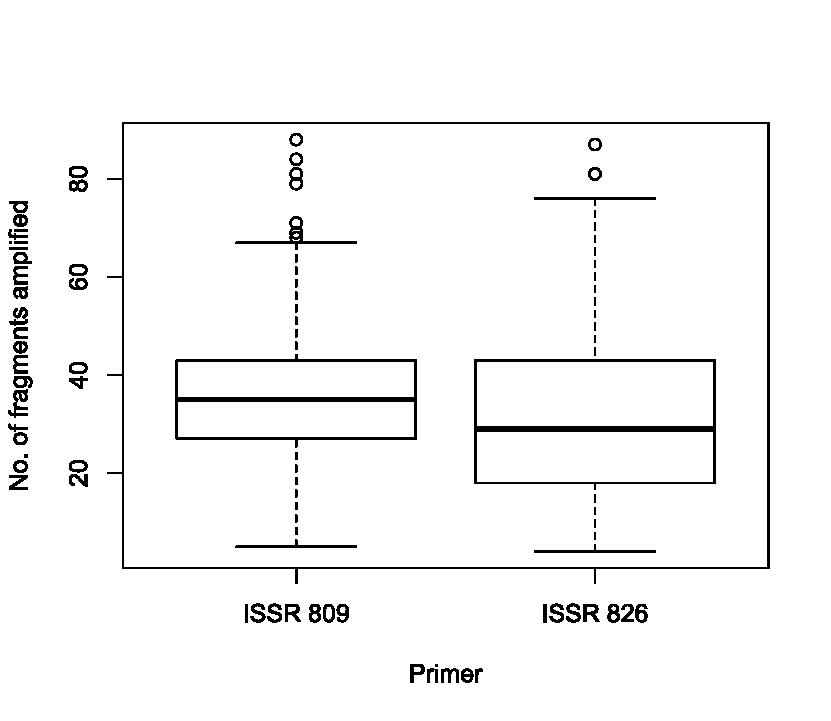
\includegraphics[scale =0.75]{Images/number_fragments_amplified.pdf}
	\caption{A box plot for the number of fragments amplified by the ISSR 809 and ISSR 826 primers.}
	\label{fig:primer_bands}
\end{figure}

% \begin{figure}[H]
% 	\centering
% 	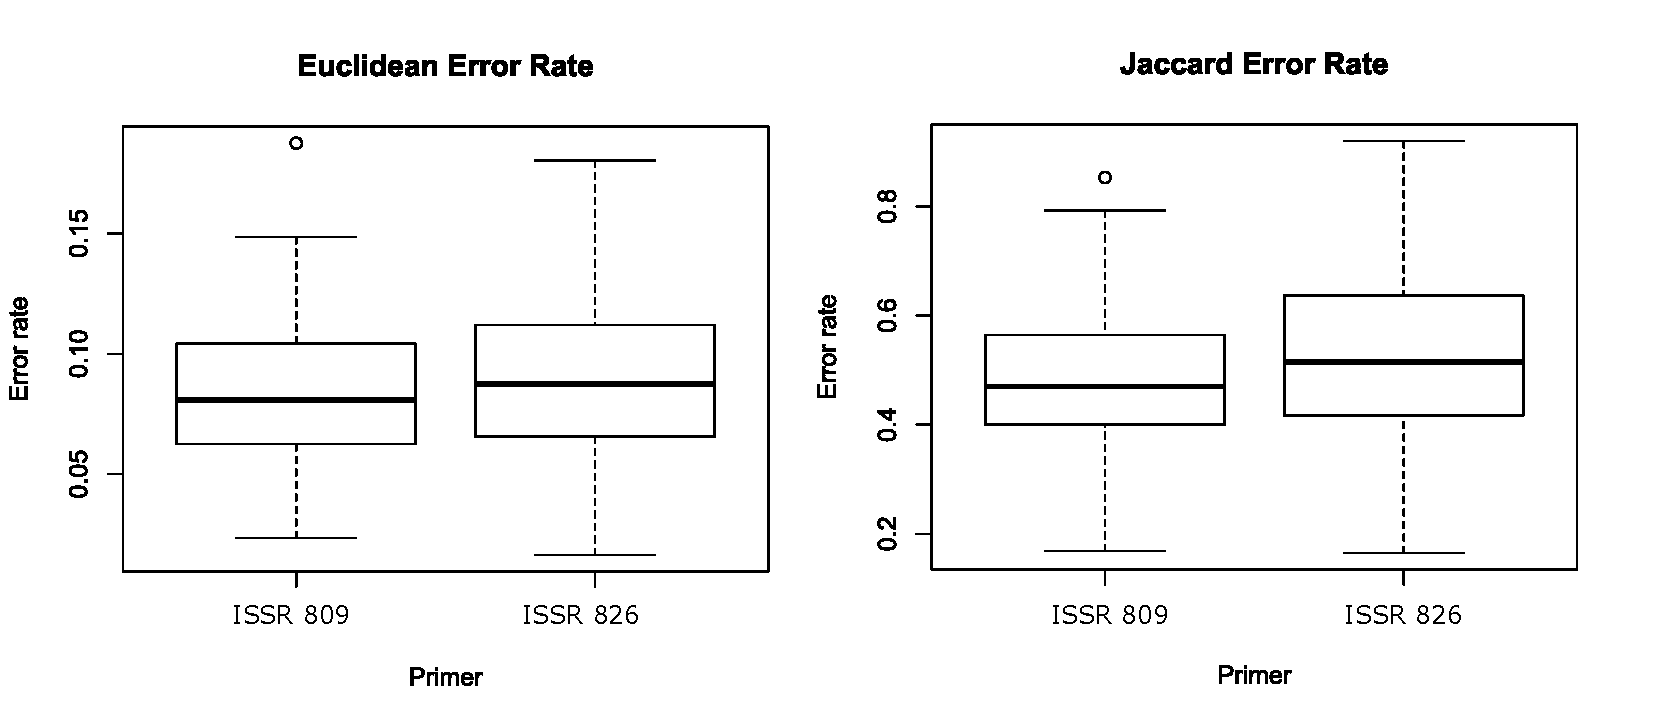
\includegraphics[scale =0.6]{Images/error_rates.pdf}
% 	\caption{Box plots for the Euclidean and Jaccard error rates for ISSR 809 and ISSR 826. Values are representative of the full data set.}
% 	\label{fig:primer_errors}
% \end{figure}

\subsection{Hierarchical clustering tree}
The UPGMA clustering tree representative of the combination of both ISSR primers showed a separation of all the \textit{Dactylopius} species (Fig. \ref{fig:issr_upgmaTree}), and corroborated the topologies in the 12S, 18S, and COI phylogenies. \textit{Dactylopius tomentosus} separated into the `californica', `imbricata', and `cholla' lineages, but `imbricata' samples split into two separate groups. The Uitenhage `ficus' and Mass Rearing Facility samples grouped together as a sister group to the Namibia `ficus' samples. The `stricta' samples from the Kruger National Park, Saudi Arabia, and samples from `stricta' source populations (kept by John Hoffmann and Hildegard Klein) separated from the `ficus' samples and from those collected in the United States. Samples from the Pecos County in Texas in the USA (VS082u and VS145) grouped with the wild `ficus' samples collected in the Eastern Cape, South Africa. Two MRF samples (Extraction IDs: VS059Os and VS063Os) grouped with samples from the USA.

\begin{figure}[H]
	\centering
	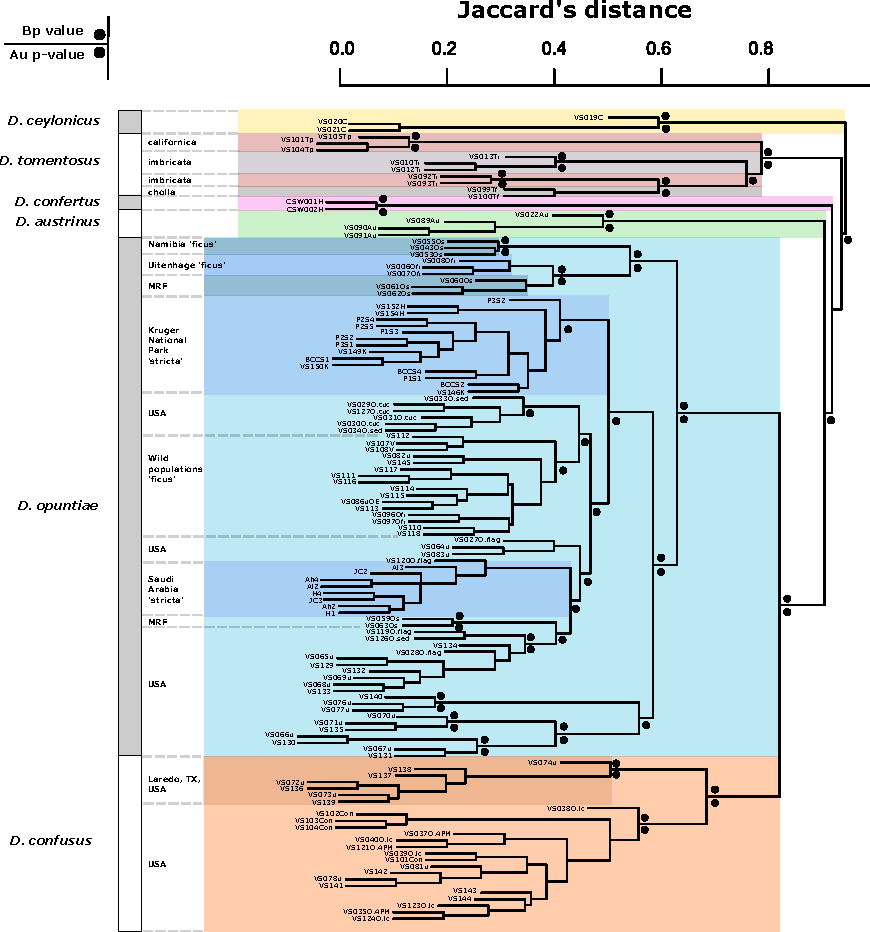
\includegraphics[height = 22cm, width = 18cm, scale =0.7]{Images/upgma_tree.pdf}
	\caption{Hierarchical clustering tree (UPGMA method) applying Jaccard's transformation for the ISSR binary data obtained from two primers (ISSR 809 and ISSR 826). Approximately unbiased p-values (Au p-value) and the bootstrap probability values (Bp-value) above 70 are shown as black dots above and below the relevant clades. One thousand bootstrap repetitions were run. MRF = Uitenhage Mass Rearing Facility.}
	\label{fig:issr_upgmaTree}
\end{figure}

\subsection{SplitsTree}
Overall, the `stricta' and `ficus' lineages showed a clear separation (Fig. \ref{fig:splitsTree}). The ANOSIM results in Table \ref{tab:ANOSIM_stats} suggest that the MRF samples were not significantly different to `ficus', but that they were to `stricta'.
The Kruger National Park and Saudi Arabian `stricta' samples separated into two groups, and the John Hoffman and Hildegard Klein samples fell into the Kruger National Park group. The wild populations, Namibian, and Uitenhage `ficus' samples also formed separate groups. See Figures \ref{fig:issr809_splitstree} and \ref{fig:issr826_splitstree} for SplitsTree diagrams for each individual ISSR primer.

\vspace{0.5cm}
\begin{figure}[H]
	\centering
	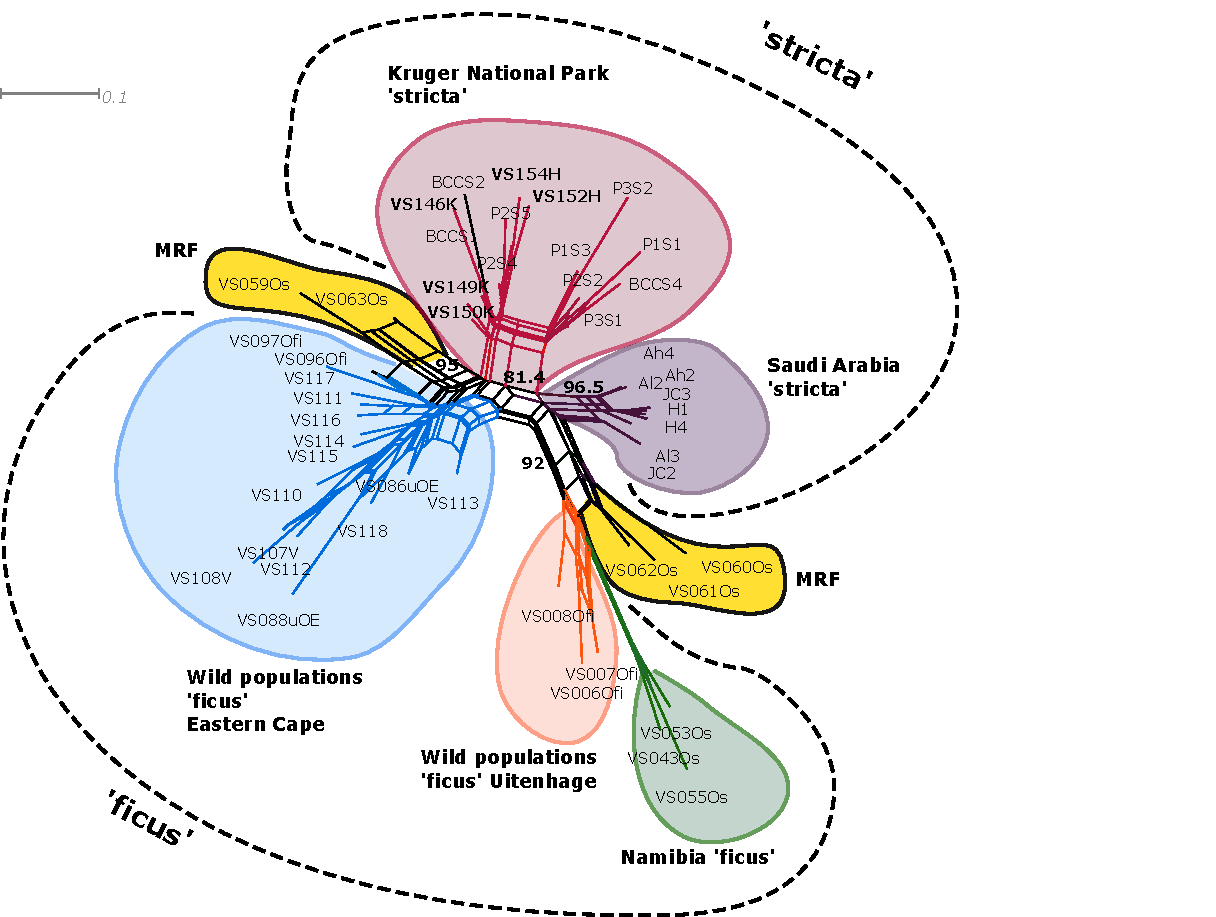
\includegraphics[scale =0.85]{Images/opuntiae_for_splitstree.pdf}
	\caption{SplitsTree graphical output (NeighborNet method, applying Jaccard's index to calculate the distance matrix) for \textit{Dactylopius opuntiae} individuals (ISSR 809 and ISSR 826). The Uitenhage and Namibia clusters are known to be the `ficus' lineage, and the Kruger National Park (KNP) contain the `stricta' lineage. Individuals in the `wild populations' group were sampled from \textit{Opuntia ficus-indica} and \textit{O. engelmannii} host plants in the Eastern Cape. MRF = the Mass Rearing Facility at Uitenhage (Eastern Cape). Bootstrap values above 75 are shown. Bold names in the KNP group denote the known `stricta' source population samples (kept by Hildegard Klein and John Hoffmann).}
	\label{fig:splitsTree}
\end{figure}

\subsection{Non-metric Multi-dimensional Scaling (nMDS) Plot}
A non-metric MDS plot (Fig. \ref{fig:2D_scatter}) showed a very similar output to the SplitsTree diagram in Figure \ref{fig:splitsTree}, with the difference of one of the Uitenhage MRF samples (VS063Os) falling within the `stricta' group. 

\vspace{0.5cm}

\begin{figure}[H]
	\centering
	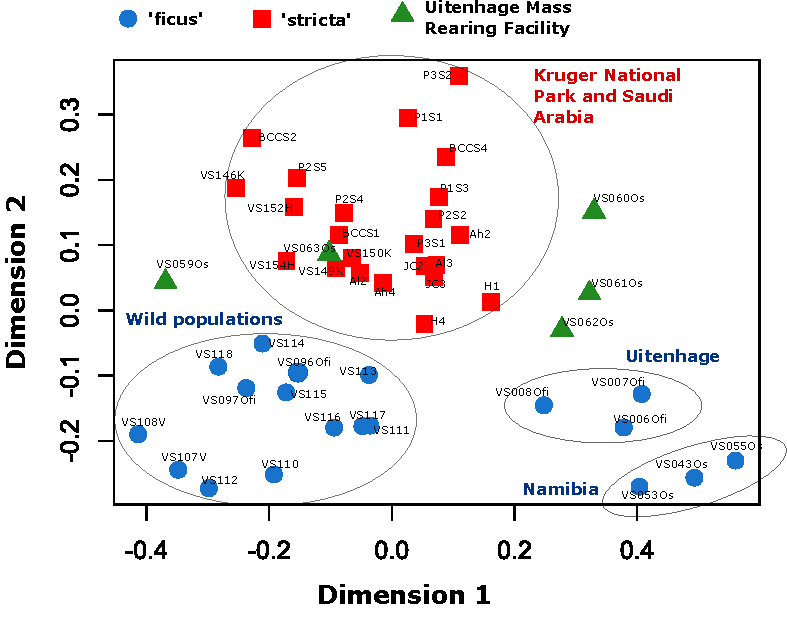
\includegraphics[scale =1.25]{Images/2d_nmds_3.pdf}
	\caption{A non-metric MDS plot based on the binary data (applying Jaccard's distance transformation) obtained from ISSR 809 and ISSR 826 to represent two different \textit{Dactylopius opuntiae} lineages. Blue circles = `ficus', red squares = `stricta', and green triangles = the Uitenhage Mass Rearing Facility.} 
	\label{fig:2D_scatter}
\end{figure}

\noindent The K = 2 dimension was applied for the nMDS plot, as the resulting stress value fell within the acceptable range (Fig. \ref{fig:shep_plots} A, B and C) \citep{dugard2010stats}. 
% Between the dimensions k = 2 and k = 3, the latter produced the lowest stress value of 0.11 compared to 0.14 (Fig. \ref{fig:shep_plots} A, B and C). The number of dimensions in a MDS analysis should ideally be kept to a minimum, and so K = 2 was applied as this stress value still falls within the acceptable range  \\
With the `ficus' group as a whole (ANOSIM: R = 0.43, p = 0.001; PERMANOVA: DF = 2, F = 6.6, R\textsuperscript{2} = 0.22, p = 0.001), and divided into known ficus samples and wild populations (ANOSIM: R = 0.72, p = 0.001; PERMANOVA: DF = 3, F = 11.69, R\textsuperscript{2} = 0.43, p = 0.001), pairwise comparisons showed that all groups were significantly different from each other (Tables \ref{tab:ANOSIM_stats}, \ref{tab:ANOSIM_stats_2}, \ref{tab:adonis_stats} and \ref{tab:adonis_stats2}). The `ficus' and MRF groups showed the greatest level of similarity (Tables \ref{tab:ANOSIM_stats} and \ref{tab:adonis_stats2}).

\begin{table}[H]
\renewcommand{\arraystretch}{0.5}
\centering
\caption{ANOSIM intra-group statistics for \textit{D. opuntiae} `stricta', `ficus' and Mass Rearing Facility (MRF) groups, showing their R values, followed by uncorrected p-values in brackets. Permutations = 999. Overall R value = 0.44, p = 0.001. Asterisks denote significance (p $<$ 0.05).}
\label{tab:ANOSIM_stats}
\begin{tabular}{@{}llll@{}}
\toprule
 & \textbf{`stricta' \scriptsize{(n = 23)}} & \textbf{`ficus' \scriptsize{(n = 21)}} & \textbf{MRF \scriptsize{(n = 5)}} \\ \midrule
\textbf{`stricta'} &  &  &  \\
\textbf{ficus} & 0.46 (0.0001)* &  & \\
\textbf{MRF} & 0.57 (0.0001)* & 0.20 (0.066) & \\ \bottomrule
\end{tabular}
\end{table}

\begin{table}[H]
\renewcommand{\arraystretch}{0.5}
\centering
\caption{ANOSIM intra-group statistics for \textit{D. opuntiae}, where the `ficus' group is split into wild populations and the `ficus' collected from around Uitenhage and in Namibia. R values are shown, followed by uncorrected p-values in brackets. Permutations = 999. Overall R value = 0.72, p = 0.001. Asterisks denote significance (p $<$ 0.05).}
\label{tab:ANOSIM_stats_2}
\begin{tabular}{@{}lllll@{}}
\toprule
 & \textbf{`stricta' \scriptsize{(n = 23)}} & \textbf{`ficus' \scriptsize{(n = 6)}} & \textbf{MRF \scriptsize{(n = 5)}} & \textbf{Wild \scriptsize{(n = 15)}} \\ \midrule
\textbf{`stricta'} &  &  &  &  \\
\textbf{`ficus'} & 0.90 (0.0001)* &  &  & \\
\textbf{MRF} & 0.57 (0.0001)* & 0.43 (0.0043)* &  &  \\
\textbf{Wild} & 0.66 (0.0001)* & 0.96 (0.0001)* & 0.74 (0.0002)* &  \\ \bottomrule
\end{tabular}
\end{table}

\begin{table}[H]
\renewcommand{\arraystretch}{0.5}
\centering
\caption{Permutational Multivariate Analysis Of Variance Using Distance Matrices for \textit{D. opuntiae} `stricta', `ficus' and Mass Rearing Facility (MRF) groups. Pairwise p-values are shown. Permutations = 999, DF = 2, F = 6.60, R\textsuperscript{2} = 0.22, p = 0.001. Asterisks denote significance (p $<$ 0.05).}
\label{tab:adonis_stats}
\begin{tabular}{@{}lll@{}}
\toprule
 & \textbf{`stricta'} & \textbf{`ficus'} \\ \midrule
\textbf{`ficus'} & 0.003* &   \\
\textbf{MRF} & 0.003* & 0.045*   \\ \bottomrule
\end{tabular}
\end{table}

\begin{table}[H]
\renewcommand{\arraystretch}{0.5}
\centering
\caption{Permutational Multivariate Analysis Of Variance Using Distance Matrices intra-group statistics for \textit{D. opuntiae} where the `ficus' group is split into wild populations and the `ficus' collected from around Uitenhage and in Namibia. MRF = Mass Rearing Facility. Pairwise p-values are shown. Permutations = 999, DF = 3, F = 11.69, R\textsuperscript{2} = 0.43, p = 0.001. Asterisks denote significance (p $<$ 0.05).}
\label{tab:adonis_stats2}
\begin{tabular}{@{}llll@{}}
\toprule
 & \textbf{`stricta'} & \textbf{ficus} & \textbf{MRF} \\ \midrule
\textbf{`ficus'} & 0.0012* & &  \\
\textbf{MRF} & 0.0012* & 0.006* &  \\
\textbf{Wild} & 0.0012* & 0.0012* & 0.0012* \\ \bottomrule
\end{tabular}
\end{table}

% With all `ficus' samples grouped (all the samples collected from \textit{O. ficus-indica} and \textit{O. engelmannii}), a one-way ANOSIM (9999 permutations applying the Jaccard similarity index) showed that the MRF samples were more similar to the `ficus' group (R = 0.20, p = 0.066) than they were to the `stricta' group (R = 0.57, p = 0.0001) (Table \ref{tab:ANOSIM_stats}). When the `ficus' group was divided into two, namely 1) the wild populations and 2) known `ficus' samples from Uitenhage and Namibia, the MRF samples were significantly different (R = 0.76, p = 0.0002) from the wild populations, and showed more similarity to the `ficus' samples from \textit{O. ficus-indica} in Uitenhage and Namibia (R = 0.43, p = 0.0043) than to `stricta' (R = 0.57, p = 0.0001). (Table \ref{tab:ANOSIM_stats_2}). `Stricta' and `ficus' showed significant dissimilarity to each other (R = 0.90, p = 0.0001). Corroborating with the Bayesian structure results (Fig. \ref{fig:struc}), the wild populations were more similar to `stricta' (R = 0.66, p = 0.0001) than to `ficus' (R = 0.96, p = 0.0001).

% \begin{figure}[H]
% 	\centering
% 	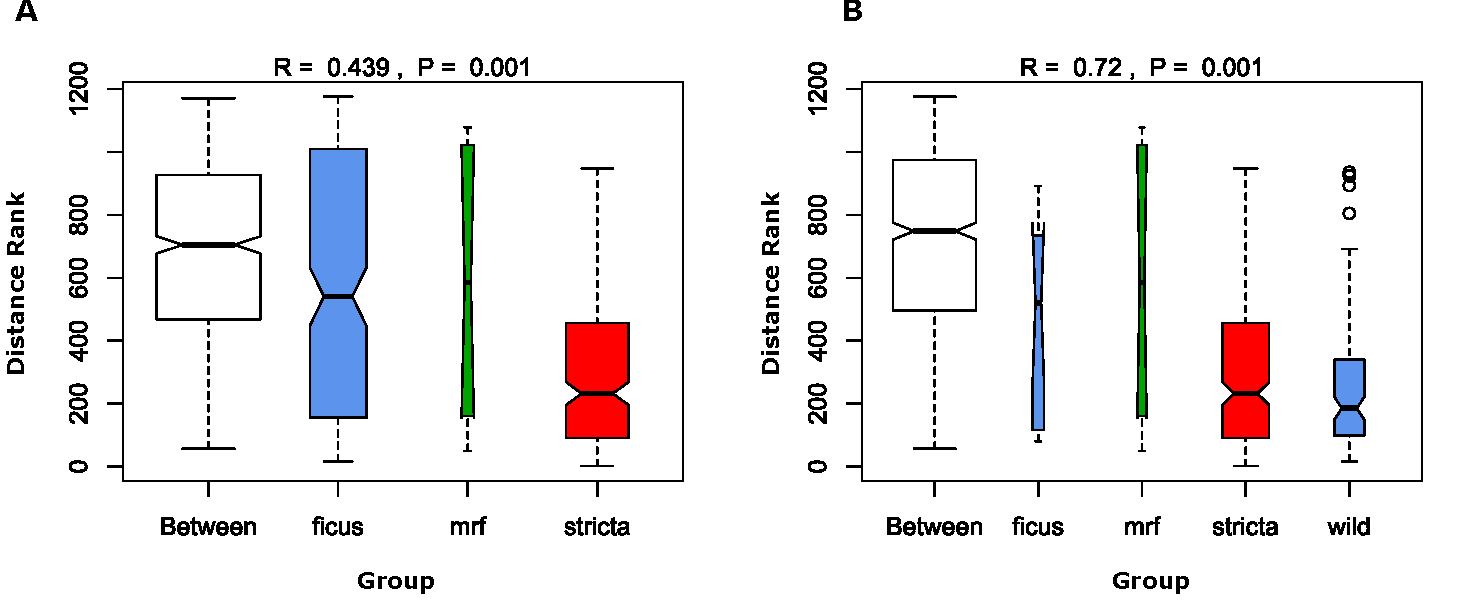
\includegraphics[scale =0.65]{Images/Anosim_opuntiae_1.pdf}
% 	\caption{Analysis of Similarity (ANOSIM) boxplots for the distances between and within A) `stricta', `ficus' and Mass Rearing Facility (MRF) groups, and B) where the `ficus' cluster is divided into samples from Uitenhage and Namibia (`ficus') and from wild populations collected in the Eastern Cape (`wild'). Black horizontal bars in the boxes indicate the median, and the bottom and top of each box represents the 25th and 75th percentile. The whiskers extend to the most extreme data points, with outliers shown as open circles. The widths of the bars are directly proportional to sample size.}
% 	\label{fig:ranked_distances}
% \end{figure}

\subsection{Structure plots}
With population data not set as priors, the \citet{puechmaille2016program} method indicated an optimal \textit{K}-value of 5, set at a threshold of 0.6, for all four tests (the MedMedK, MedMeanK, MaxMedK and MaxMeanK). The \citet{evanno2005detecting} method indicated optimal \textit{K}-values of 2 and 6 according to the $\Delta$\textit{K} and mean LnP(\textit{K}) methods, respectively. \\
When population data were set as priors, the \citet{puechmaille2016program} method gave the same output as above, except that the \citet{evanno2005detecting} method gave the optimal \textit{K}-value as being 2 for the $\Delta$\textit{K} method, and 5 for the mean LnP(\textit{K}) method. Clusters \textit{K} = 2 and \textit{K} = 5 are presented in the resulting Structure plots (Fig. \ref{fig:struc}). 
In both Structure plots (with and without priors), when \textit{K} = 2, the Saudi Arabia, Kruger National Park and Klein and Hoffmann source populations of `stricta' formed one shared cluster (light blue). The Uitenhage and Namibia `ficus' and three of the MRF samples formed a second cluster (orange). Two of the MRF samples shared the same cluster group as `stricta'. When forced into one of two clusters, the wild `ficus' populations were more genetically similar to the `stricta' cluster than they were to `ficus' samples. \\
When \textit{K} = 5, the Kruger National Park and Klein and Hoffmann source population `stricta' samples formed one cluster (maroon) (Fig. \ref{fig:struc}). The Uitenhage `ficus' and three of the MRF samples formed a separate cluster (orange). The remaining two MRF samples shared a cluster with the wild `ficus' populations (light blue). The MRF samples shared some similarity to the Kruger National Park and Saudi Arabian `stricta' clusters. The Saudi Arabian `stricta' (dark purple) and Namibian `ficus' (green) formed their own separate clusters. Taking into account Figures \ref{fig:splitsTree} and \ref{fig:struc}, individuals from the Uitenhage MRF appear to be either a hybrid of the `stricta' and `ficus' lineages, or they fall within the `ficus' group. 

\subsection{Identification accuracy}
At the species level, at an optimal threshold of 60\%, all barcode tests (BCM, TID, and NN) had a 100\% IA (Table \ref{tab:issr_barcode_results}). At the lineage level, at an optimal threshold of 45\%, \textit{D. tomentosus} had an IA of 100\% for both the BCM and TID tests (Table \ref{tab:issr_barcode_results}). At the same 45\% threshold, \textit{D. opuntiae} had an IA of 81.82\% (no ID of 18.18\%) for both the BCM and TID tests.

\vspace{0.5cm}
\begin{table}[H]
\renewcommand{\arraystretch}{0.5}
\caption{Barcode testing results for the Best Close Match (BCM), Threshold ID (TID), and Nearest Neighbour (NN) tests, at the species and lineage level.}
\label{tab:issr_barcode_results}
\resizebox{\columnwidth}{!}{%
\begin{tabular}{lllllllll}
\hline
 &  & \textbf{BCM} & \textbf{\% of samples} & \textbf{TID} & \textbf{\% of samples} & \textbf{} & \textbf{NN} & \textbf{\% of samples} \\ \hline
\textbf{SPECIES LEVEL} & \textbf{} & \textbf{60\% threshold} &  & \textbf{60\% threshold} &  &  &  &  \\
 & \textbf{Correct} & 124 & 100 & 124 & 100 & \textbf{True} & 124 & 100 \\
\textbf{} & \textbf{No id} & 0 & 0 & 0 & 0 & \textbf{False} & 0 & 0 \\
 & \textbf{} &  &  &  &  & \textbf{} &  &  \\
\textbf{LINEAGE LEVEL} & \textit{\textbf{D. tomentosus}} & \textbf{45\% threshold} &  & \textbf{45\% threshold} &  & \textbf{} &  &  \\
 & \textbf{Correct} & 10 & 100 & 10 & 100 & \textbf{True} & 10 & 100 \\
 & \textbf{Incorrect} & 0 & 0 & 0 & 0 & \textbf{False} & 0 & 0 \\
\textbf{} & \textbf{Ambiguous} & 0 & 0 & 0 & 0 &  &  &  \\
 & \textit{\textbf{}} &  &  &  &  &  & \textbf{} &  \\
 & \textit{\textbf{D. opuntiae}} & \textbf{45\% threshold} &  & \textbf{45\% threshold} &  &  &  &  \\
 & \textbf{Correct} & 36 & 81.82 & 36 & 81.82 & \textbf{True} & 44 & 100 \\
 & \textbf{Incorrect} & 0 & 0 & 0 & 0 & \textbf{False} & 0 & 0 \\
 & \textbf{Ambiguous} & 0 & 0 & 0 & 0 &  &  &  \\
 & \textbf{No id} & 8 & 18.18 & 8 & 18.18 &  & \textbf{} & \\ \bottomrule
\end{tabular}
}
\end{table}

\vspace{0.5cm}
\begin{figure}[H]
	\centering
	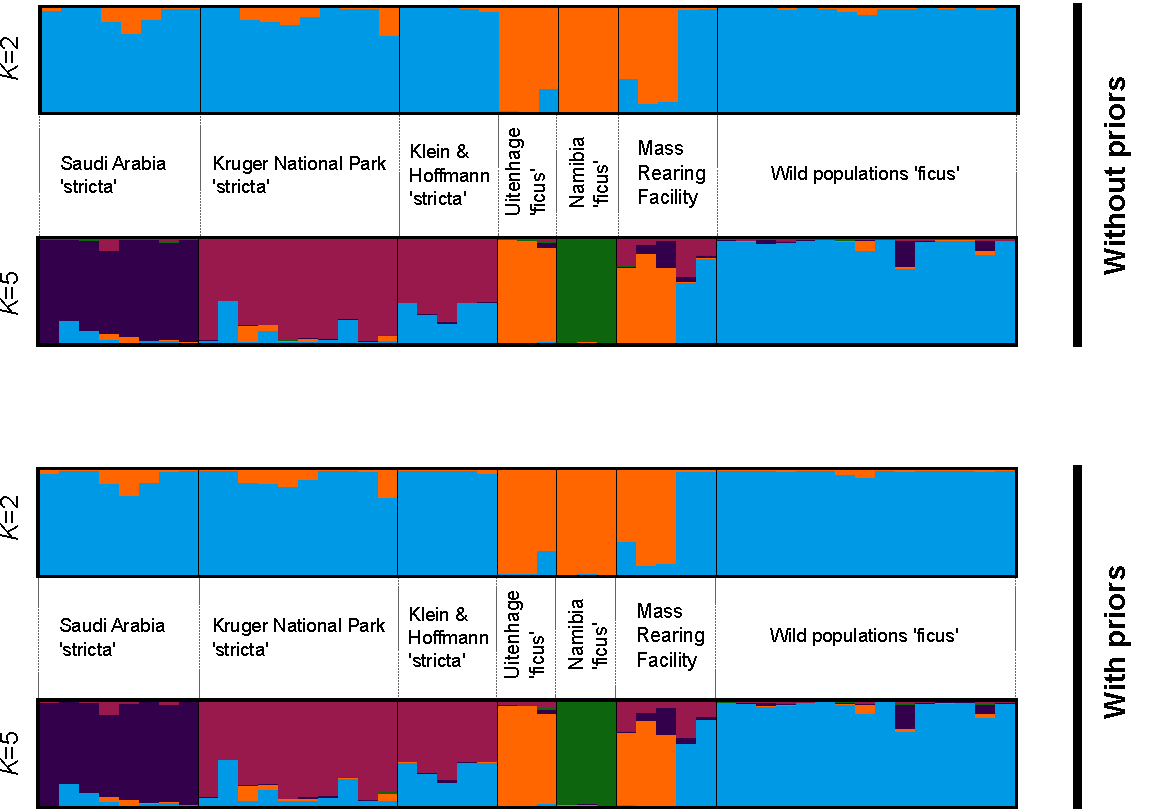
\includegraphics[scale =0.9]{Images/structure_diagrams.pdf}
	\vspace{0.2cm}
	\caption{STRUCTURE results using Bayesian analysis (MCMC = 50 000, burn-in = 100 000), showing genetic clustering patterns for \textit{Dactylopius opuntiae} individuals. Results for both \textit{K} = 2 and \textit{K} = 5 are shown for runs with and without priors.}
	\label{fig:struc}
\end{figure}


%\end{landscape}


\chapter{Discussion}

% This study aimed to generate multi-locus genetic barcoding data for the identification of the species and lineages within the \textit{Dactylopius} genus. Of particular interest were the lineages within \textit{Dactylopius opuntiae}, namely `ficus' and `stricta', used for the control of \textit{Opuntia ficus-indica} and \textit{Opuntia stricta}, respectively, and a number of \textit{D. tomentosus} lineages used for the control of invasive \textit{Cylindropuntia} species. Successful biological control programmes rely on the correct identification of control agents, as different species and intraspecific lineages can offer varying levels of control efficacy. The output of this project is thus highly valuable to programmes aimed at controlling invasive Cactaceae using \textit{Dactylopius} agents. \\
This chapter summarises and explains the results obtained from two mitochondrial regions, one nuclear gene region, and two ISSRs used to assess the identification accuracy of the Dactylopiidae using both tree-based methods and barcode testing algorithms. It also discusses aspects relating to geographical distribution, and the practical applications arising from this thesis.

\section{Genetic markers}
\subsection{12S}

The 12S rRNA genetic marker provided 100\% identification accuracy (IA) at both the species level (at a 1\% genetic distance threshold) and for three of the six \textit{D. tomentosus} lineages (at a 0.2\% genetic distance threshold) using barcode testing algorithms. Bayesian (BI) and Maximum Likelihood (ML) phylogenies supported this result, showing well-supported clades that distinguished all species. Both standard and secondary structure RNA alignment methods suggest that this marker can accurately distinguish between the `californica', `cholla', and `imbricata' lineages, but that the `echinocarpa x acanthocarpa', `bigelovii', and `cylindropuntia spp.' samples form one clade. \\
The BI tree showed a well-supported separation between South African and Australian \textit{D. ceylonicus} samples. This is most likely due to the fact that the species was released in South Africa and Australia in 1913 and 1914, respectively, and have been isolated from each other for more than a hundred years. The agents used in these two releases came from the same stock, which were originally collected in Brazil, then exported to India, and subsequently to Sri Lanka \citep{Winston2014BiologicalWeeds.}. \textit{Dactlopius austrinus} and \textit{D. tomentosus} `imbricata' and `cholla' did not show the same separation between the two countries, most likely because they have not been separated for long enough. \\ 
The 12S rRNA primers successfully amplified the target region of five of the six \textit{Dactylopius} species used in this project (only \textit{D. confertus} was unsuccessful), and had the highest mean between-group K2P distance (0.30 $\pm$ 0.14). The marker is not, however, useful for distinguishing between \textit{D. opuntiae} `ficus' and `stricta' lineages, due to the presence of negative barcode gaps (i.e. intraspecific variation $>$ interspecific variation) at that higher resolution taxonomic level. The BI tree aligned according to the secondary structure of RNA did not vary greatly from the standard alignment, but did show stronger support for a single clade containing the \textit{D. tomentosus} `echinocarpa x acanthocarpa' and `bigelovii' lineages that was separate from the `cylindropuntia sp.' samples.  \\
A number of other studies have found the 12S rRNA marker highly useful for DNA fingerprinting, such as for the identification of ticks (Acari: Ixodida) \citep{lv2014assessment}, earthworms (Lumbricidae) \citep{klarica2012comparing}, commercial fishes \citep{ardura2010dna, hardy2011dna, cawthorn2012evaluation}, snakes (from venom samples) \citep{pook2005mitochondrial}, and various animal species used in traditional medicines \citep{luo2011application}.
Based on the results of this study, and due to the ease of PCR amplification of the Dactylopiidae using this gene region, it is recommended as the most efficient for species-level identification, and for the identification of the `cholla', `californica', and `imbricata' lineages within the \textit{D. tomentosus} species.

\subsection{18S}
The 18S rRNA marker could accurately distinguish between all \textit{Dactylopius} species, except for \textit{D. austrinus} and \textit{D. ceylonicus}, which grouped into one clade and were the only two species with negative barcode gaps. This may suggest a more recent speciation event between these two species, relative to the others. The overall IA was 94.59\% at the species level. The primers successfully amplified the target region of all six \textit{Dactylopius} species used in this study. The genetic distance threshold for this marker was lower (0.2\%) for species level identification, and had the lowest mean between-group K2P distance (0.03 $\pm$ 0.02) owing to the slow evolutionary rate in this nuclear gene relative to mitochondrial regions. \citet{evans2007assessment}, for example, tested COI, rbcL, 18S and ITS rDNA as potential barcoding regions, and found that 18S was the least variable marker. \\
Of the \textit{D. tomentosus} lineages, only `cholla', and `echinocarpa x acanthocarpa' and `bigelovii' formed separate clades, while `imbricata', `californica', and `cylindropuntia' were unresolved. In their study of Murray-Darling Basin fishes, \citet{hardy2011dna} found that the 18S rRNA marker could successfully identify 83.1\% of the species sampled, but that there were a number of different species within a genus complex that shared identical sequences. In the study by \citet{Campana2015}, no intraspecific variation was found within the seven sequences obtained from \textit{D. coccus} populations. This corroborates the findings of the current project, namely that this marker is uninformative for identification beyond the species level. It can, however, be used for the inference of phylogenetic relationships between species, particularly when supplementing a concatenated genetic data set.

\subsection{COI}
COI-A primers could distinguish between \textit{D. confertus}, \textit{D. opuntiae}, and \textit{D. confusus} with a 100\% IA. A 1\% genetic distance threshold was found to be to be optimal for assessing identification accuracy at the species level, which is consistent with the barcoding literature \citep{Hebert2003, Hebert2003a}. It is not, however, able to distinguish between \textit{D. opuntiae} lineages. When barcode accuracy was tested at the lineage level, all \textit{D. opuntiae} sequences displayed negative barcode gaps (intraspecific variation $>$ interspecific variation) due to the high similarity between the `ficus' and `stricta' lineages. 
The average within-group p-distance was similar to that of the 12S region (0.22 $\pm$ 0.1). \\
COI-B primers successfully amplified all \textit{D. tomentosus} lineages. At a genetic distance threshold of 3.3\%, IA increased from 70.37\% to 100\% when the `echinocarpa x acanthocarpa', `bigelovii', and `cylindropuntia sp.' lineages were treated as one lineage. ISSR analyses for these particular lineages may reveal further differences between them. 

\section{Distance-based barcode testing}

In agreement with \citet{Birch2017TestingAustralia}, the TID barcode testing algorithm is the more conservative test, and is recommended as the most appropriate since it takes into consideration a genetic distance threshold. It, therefore, reduces the number of false positive identifications, as opposed to the NN and BCM tests. The NN algorithm was mostly an inappropriate measure in the context of this study, particularly with reference to the lineage level where genetic similarity was very high. 
% For example, the 12S marker showed a TID hit rate of only 13.04\% for \textit{D. opuntiae} lineages at a 0.2\% threshold, but the NN showed a 80.43\% accuracy rate. 
Since each gene evolves at a different rate, a one-size-fits-all approach of a default 1\% distance threshold is inaccurate. Combining appropriate distance and tree-based methods to determine barcoding accuracy offers a more thorough approach to the identification of target taxa.

\section{Posterior probabilities vs bootstrap values}

Some clades in the phylogenies in this study showed much higher bayesian posterior probability (BPP) support than their corresponding ML bootstrap values. This is not uncommon, and stems from the fact that these two methods assess data in fundamentally different ways and are based upon different statistical assumptions \citep{huelsenbeck2002potential, douady2003comparison, garcia2004comparison, huelsenbeck2004frequentist}. \citet{huelsenbeck2002potential} suggest that the ML bootstrap method underestimates the confidence of phylogenetic clades, and propose that a Bayesian analysis is the most easily interpretable and accurate given the correct evolutionary models. In a simulation, \citet{alfaro2003bayes} found that the greatest disparity between BPP and bootstrap values occurred when the branch lengths were short, or when the number of characters available for comparison was small. They suggest that a Bayesian analysis offers a greater sensitivity to phylogenetic signal, and that a substantial increase in the number of characters will facilitate the convergence of bootstrap values to BPP. \\ 
% The 12S sequences were the shortest of the four genetic markers, at $\sim$ 413 base pairs in length in the final alignment (compared to 18S with $\sim$ 570 base pairs, PCOF1 and LepR1 with $\sim$ 526 and DTOMf and HCO2198 with $\sim$ 546 base pairs). This could be a contributing factor to the differences in support values between the BI and ML trees. 
A study by \citet{hardy2011dna} used the 12S rRNA region (in addition to 18S rRNA and the mtDNA control region (CR)) to differentiate between different fish species in the Murray-Darling River Basin in Australia. The BI and ML analyses did not differ substantially in their support values, but they did report that the 12S trees in particular showed greater variability (where a number of clades had bootstrap support values $<$ 75 and BPP $>$ 95). Similarly, a study by \citet{wilcox2002phylogenetic} analysed the 12S, 16S, and valine-tRNA gene regions of dwarf boa snakes (Tropidophiidae), and found that some branches in their 12S and 16S phylogenies had BPP values more than double that of the corresponding bootstrap support values. Based on their results, the authors recommended the use of Bayesian analyses above bootstrapping methods, as it provided a more reliable estimation of phylogenetic accuracy. The present study supports this statement, especially taking into account the faster computational time that a Bayesian analysis offers compared to other methods \citep {huelsenbeck2001bayesian, douady2003comparison}.

\section{ISSR fragment analysis}
The percentage of polymorphism found in this study was lower than that reported by \citet{silva2013genetic}, who collected \textit{D. opuntiae} on \textit{O. ficus-indica} host plants in the native range in northeast Brazil. 
% For example, the present study reported a percentage polymorphism average of 22 and 38.53\% for `stricta' and `ficus', respectively, compared to the 71.4\% polymorphic loci for ISSR 809 ((AG)\textsubscript{8}C), and a maximum of 87.5\% for the TCT(GA)\textsubscript{7} primer reported in their study. 
Their overall polymorphism percentage was 70.9\%, taken as an average of nine different ISSR primers. The present study reported only 44.93\% polymorphism. Additionally, they reported a genetic similarity of 80\% across all populations. Comparatively, the present study reported an average Jaccard similarity of 51.67\% (SE $\pm$ 1.01) for all \textit{D. opuntiae} samples. This is arguably due to the higher number of fragments reported in the present study due to the use of DNA fragment analysis using capillary electrophoresis. Over three-fold more fragments were found per primer than by \citet{silva2013genetic}, who scored fragments manually through visualising bands on agarose gels. 
\citet{silva2013genetic} used both ISSR and RAPD primers to distinguish between \textit{D. opuntiae} populations, and concluded that the RAPD primers used were more effective than ISSRs in grouping populations, but neither method succeeded in discriminating between populations from different geographic regions. \\
The \textit{D. opuntiae} ISSR data using Bayesian and ordination methods showed a statistically significant difference between the `ficus' and `stricta' lineages that the traditional DNA gene regions failed to reveal. The methods also showed significant differences between \textit{D. opuntiae} `ficus' populations; namely wild populations collected on \textit{O. ficus-indica} and \textit{O. engelmannii} in the Eastern Cape, and specimens collected from \textit{O. ficus-indica} around the Uitenhage Mass Rearing Facility (MRF) and in Namibia. 

\subsection{`Stricta' and `ficus' lineages}

\subsubsection{Eastern Cape wild populations}
An unexpected result arising from the Bayesian Structure analysis (and supported by the nMDS ordination grouping) was that when forced into one of two cluster groups, the wild `ficus' populations collected from \textit{O. ficus-indica} and \textit{O. engelmannii} in the Eastern Cape were more genetically similar to the `stricta' cluster than they were to known `ficus' samples. It is possible that the wild populations have regularly hybridised with `stricta' and `ficus' lineages (hybridisation between these two lineages is reported in the work by \citet{Hoffmann2002BiologicalBiotypes} and  \citet{Hoffmann2004}), and that the genotypic status detected by the two specific ISSR primers used in this study currently aligns more with that of `stricta'. Collecting more specimens from \textit{O. ficus-indica} and \textit{O. engelmannii} in more distant regions of the country (in addition to the Namibian samples included in this study that grouped in the `ficus' cluster) could provide further clarity. When forced into one of five cluster groups, the wild populations did represent a distinct genotypic cluster not shared by any of the `stricta' genotypes. 


\subsubsection{Uitenhage Mass Rearing Facility (MRF)}
The \textit{D. opuntiae} population believed to be of the pure-bred `stricta' lineage at the MRF were more similar to `ficus' samples collected from \textit{O. ficus-indica} growing around the facility and from Namibian samples than they were to `stricta' samples. The MRF individuals are either the result of crosses between the two lineages, or they are merely part of the `ficus' group. This suggests that contamination has taken place, and that the control efficacy of the hybrid individuals being reared may be compromised. It is recommended that 1) the current culture be destroyed, and replaced with a new colony that is known to be the `stricta' lineage, 2) the wild `ficus' populations around the MRF should be killed, and 3) the genetic status of the colonies be checked on a regular basis to ensure that a pure-bred lineage is maintained. Additionally, it would be worth crossing and backcrossing the pure `stricta', `ficus', and MRF populations to test their host-specificities.

\subsubsection{The Kruger National Park and Saudi Arabia}
The \textit{D. opuntiae} samples from the Kruger National Park shared a genotypic cluster with the known `stricta' source populations (kept by Hildegard Klein and John Hoffmann), and were different from the `ficus' clusters. It could therefore be confirmed that these samples were of the `stricta' lineage. Similarly, the Saudi Arabian \textit{D. opuntiae} samples collected from \textit{O. stricta} shared a genetic cluster with the `stricta' source populations; confirming their identity as well. These populations can therefore effectively control \textit{O. stricta} \citep{githure1999host, Volchansky1999}, and can be mass reared if necessary. These populations can also be used as a source for the new clean culture of `stricta' at the Uitenhage MRF.

\subsection{ISSR identification accuracy}
Due to the different kind of data that ISSR analyses produce, the distance threshold required to create species group designations was much higher than that of nucleotide sequence data (60\% compared to the standard 1\%). This is because the latter is much more data-rich compared to binary information. \\
The identification success rate for \textit{D. opuntiae} lineages was 81.82\% at a 45\% distance threshold, with the remaining 18.18\% falling into the `No ID' category.  ISSR analysis using the methods described in this work offers a new and valuable tool to biological control efforts, as it allows practitioners to distinguish between these otherwise morphologically identical lineages. The \textit{D. tomentosus} lineages included in the ISSR analyses (`imbricata', `cholla', and `californica') showed a 100\% IA at a distance threshold of 45\%, although using the 12S rRNA marker to identify these is less labour intensive. \\
Of the two ISSR primers used, ISSR 826 had an average Jaccard error rate 5\% greater than ISSR 809, and tended to be less informative for some population groups compared to the latter primer. The average Euclidean error rates of 0.08 ($\pm$ 0.03) and 0.09 ($\pm$ 0.03) for ISSR 809 and ISSR 826, respectively, were in the same range as that found by \citet{paterson2013issrs} for \textit{Chromolaena odorata}. Whether the shared absence of bands is included in the error rate calculation can greatly impact its interpretation, and so it is important that future studies include both the Euclidean and Jaccard error rates for comparison. The present study reported average Jaccard error rates 6-fold greater than their Euclidean equivalent, which is comparable to those found by \citet{holland2008optimizing}, who reported a 4-fold difference in one experiment. \\
Although a 81.82\% hit rate is high for the identification of \textit{D. opuntiae} lineages, there are a multitude of other ISSR primers that may offer lower error rates and amplify a larger number of fragments. It would be worth using capillary electrophoresis to test the TCT(GA)\textsubscript{7} ISSR primer reported by \citet{silva2013genetic} as producing the highest percentage of polymorphic loci, and to test the RAPD primers used in their study.

% \subsection{Australian \textit{D. tomentosus} lineages}
% Both the 12S rRNA and COI (DTOMf \& HCO2198) markers clearly distinguished between the `californica', `cholla' and `imbricata' lineages, and showed that the `echinocarpa x acanthocarpa' and `bigelovii' lineages grouped into one clade due to their high level of genetic similarity. Support for the `cylindropuntia sp.' samples forming their own distinct clade was ambiguous. There is more support for them forming part of the `echinocarpa x acanthocarpa'/bigelovii' clade. ISSR analyses may offer further resolution in this case.

\section{Geographical distribution}
The first phylogeny for the Dactylopiidae was constructed by \citet{Perez-Guerra1992} using morphological data. The authors concluded that all the \textit{Dactylopius} species derived from one common ancestor, that \textit{D. coccus} was the most basal species, and that \textit{D. ceylonicus} was the most derived. \citet{Rodriguez2001} later created a phylogeny based on both morphological traits and geographical distributions, which formed two clades separating North and South American species. The results from the present study, and those from a molecular analysis by \citet{Ramirez-Puebla2010MolecularBacteria} (using the same 12S and 18S genetic markers), did not find this well-defined separation between the northern and southern continents (Fig. \ref{fig:phylogeny_comparison}). 
Both studies did, however, agree with the finding that \textit{D. tomentosus} was the most different from the other species. This is expected, because \textit{D. tomentosus} has a considerably different life history and morphological characteristics \citep{Perez-Guerra1992, Mathenge2009}.
The present results also agree with \citet{Rodriguez2001}'s finding that \textit{D. austrinus} and \textit{D. ceylonicus} are very closely related. These are both South American species. \\
Conflicting results between morphological phylogenies have been reported for this genus \citep{Portillo2006AENEMIES}, and  numerous other studies have reported on what is termed the `morphological-molecular conflict' \citep{cohen2018match}. Morphological phylogenies can be misleading due to the convergent evolution of traits, as homologous morphologies are not necessarily the result of homologous genes \citep{cartmill1994critique}. \citet{cohen2018match}, for example, states that \textit{ `morphological characters are only indirectly genealogical...and are intrinsically not capable of reporting evolutionary history'}. \\
The absence of a clear north-south geographic divide between the Dactylopiidae species is not unexpected, since the Cactaceae evolved in South America about 65 mya (some studies have suggested ranges between 100 \citep{mauseth1990continental} and 30 mya \citep{hershkovitz1997evolutionary}) following the Gondwana split, and only later dispersed northwards \citep{Anderson2001}. The North and South American continents were only connected by land (the Isthmus of Panama) about 5.7 mya, and so dispersal to the north prior to that is debatable \citep{Anderson2001, portillo2007biogeography}.
It is possible that some cacti dispersed via island bridges formed by the Central American Volcanic Arc, and rafting prior to the land connection \citep{Anderson2001}, and it has also recently been proposed that the Isthmus of Panama may have in fact formed 13 to 10 mya \citep{montes2015middle}. Thus the palaeontological event known as the `Great American Biotic Interchange' (GABI) may have occurred much earlier; although these are only hypotheses. \\
Based on the particular gene regions used in this study, which are also supported by the findings of \citet{Ramirez-Puebla2010MolecularBacteria}, it may be that there were multiple dispersal events of the Dactylopiidae from South to North America at different times. And that these founder populations proceeded to speciate in North America.
This raises interesting questions around the coevolution between the Cactaceae and the Dactylopiidae, and the role that human-mediated dispersal had to play in the insects' current distribution.
The evolutionary history of the Cactaceae and the Dactylopiidae is still very poorly understood, and matters are made still more confusing by records of South American \textit{D. ceylonicus} in Mexico, and North American \textit{D. confusus} in Peru \citep{portillo2007biogeography}. Disentangling human-mediated from natural dispersal events is very challenging.
It would be valuable to include \textit{D. gracilipilus}, \textit{D. salmianus}, and \textit{D. zimmermannii} in the current analysis to create a complete phylogeny (at least for the currently described species), and to compare that to the phylogeny of their associated host plants. This could shed further light on host-plant evolutionary dynamics.

\begin{landscape}

\begin{figure}[]
	\centering
	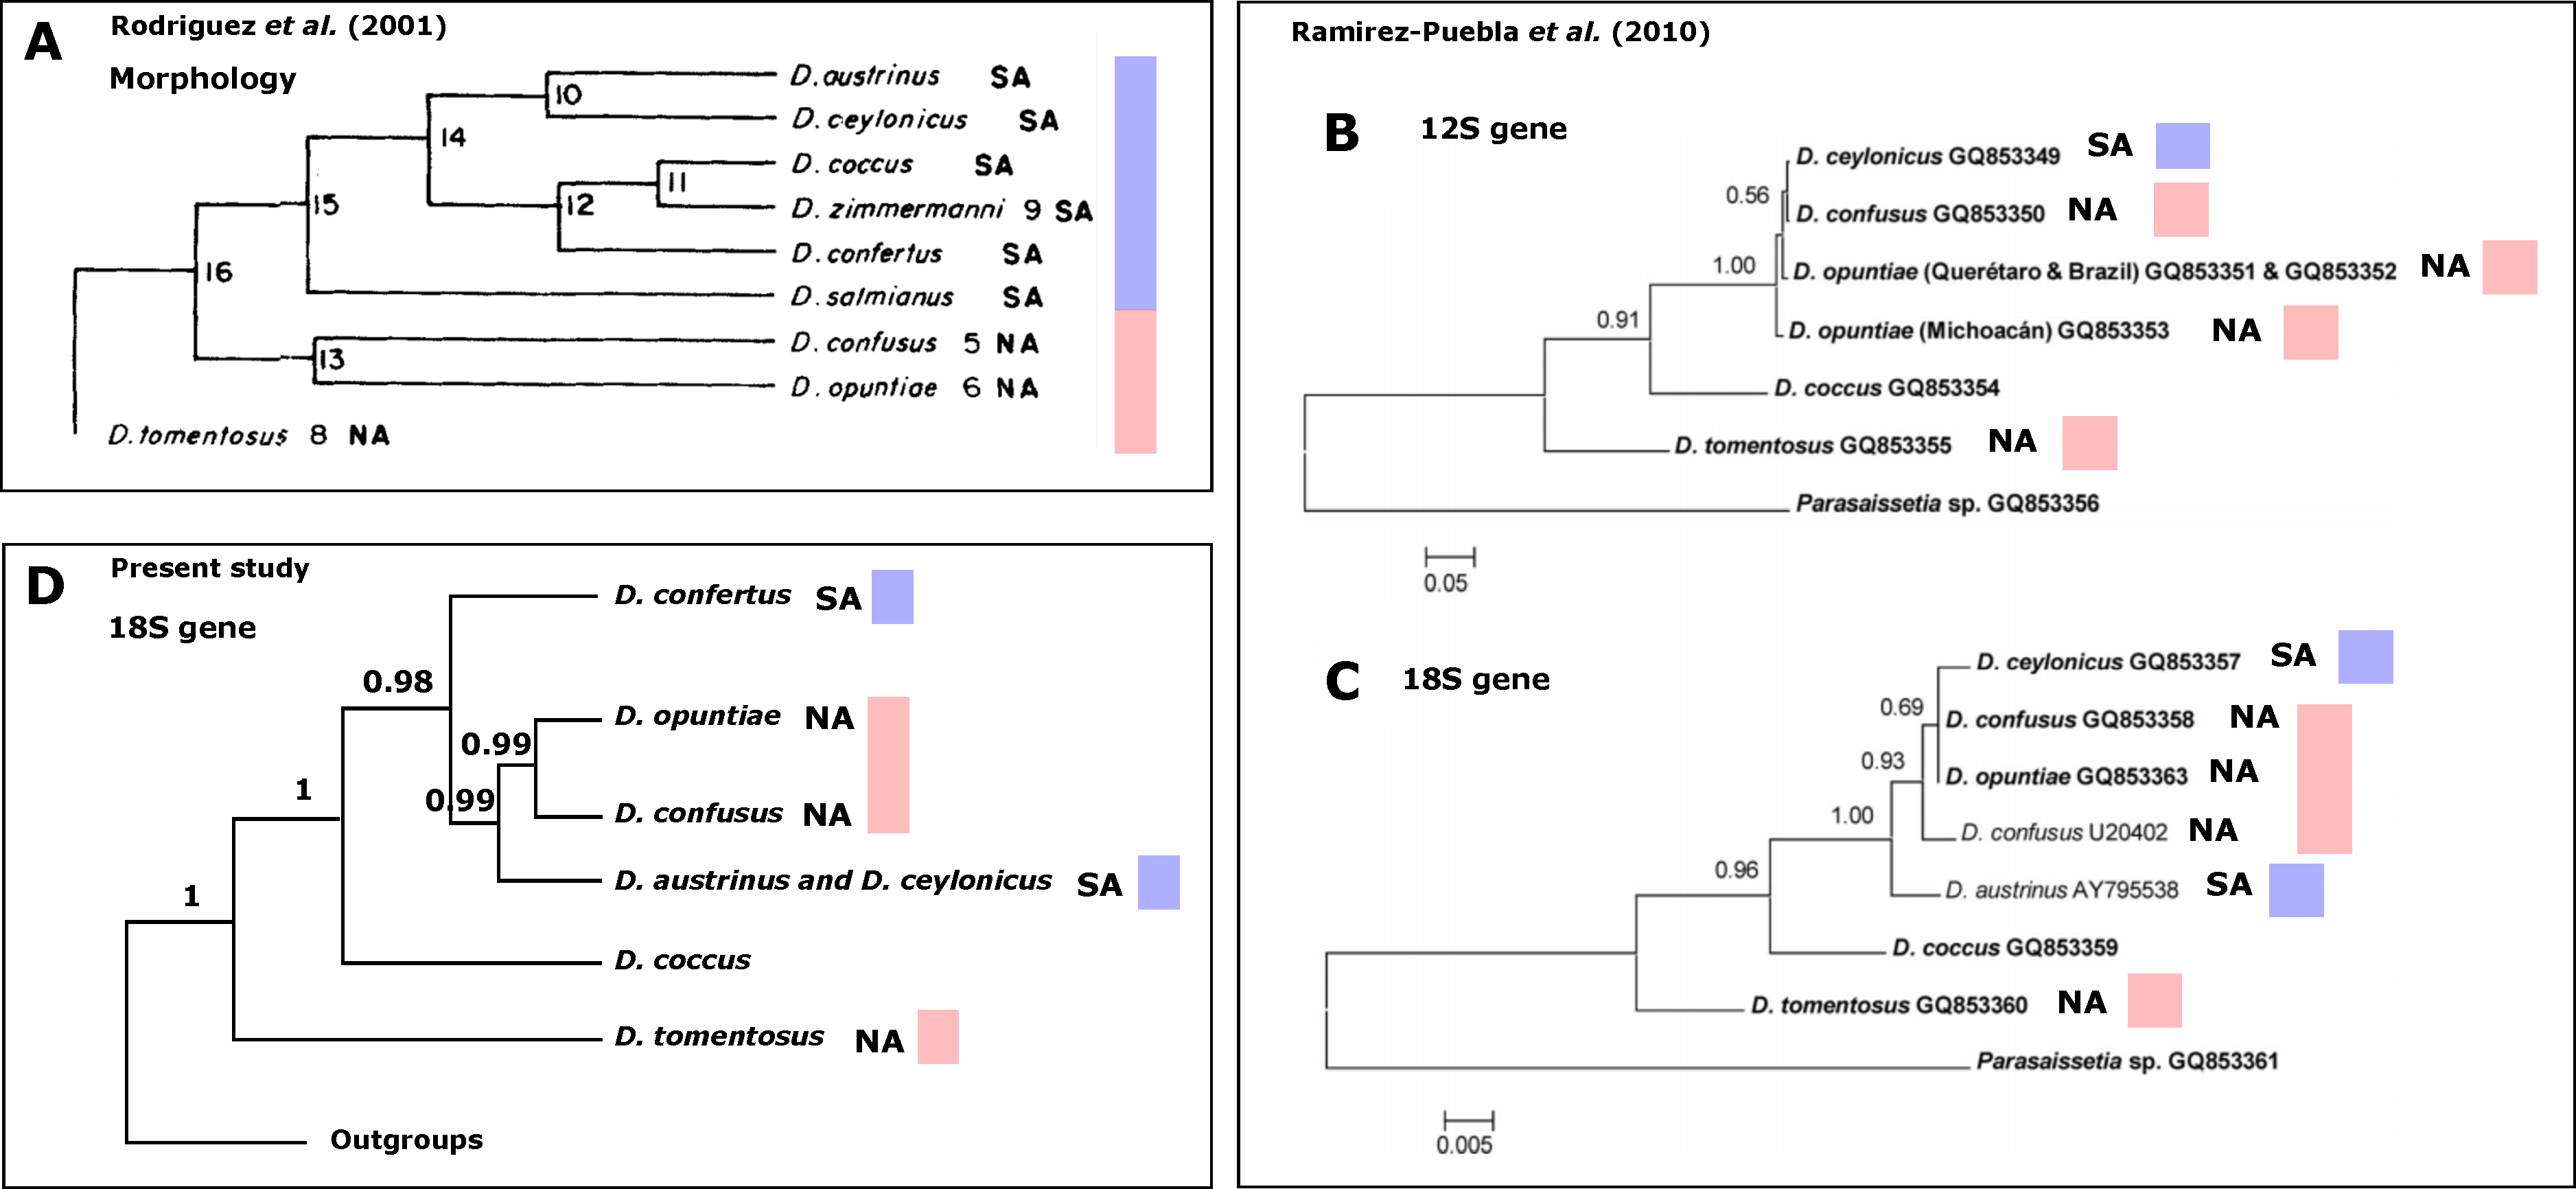
\includegraphics[scale =0.38]{Images/phylogeny_comparison.pdf}
	\caption{A comparison of the phylogenies produced by A) \citet{Rodriguez2001} based on morphological characteristics, \citet{Ramirez-Puebla2010MolecularBacteria} based on the B) 12S and C) 18S rRNA gene regions, and D) the present study, represented as a cladogram for the 18S region (not to scale). The values on the branches of diagrams B, C, and D are Bayesian posterior probability values. NA = North America; SA = South America.} 
	\label{fig:phylogeny_comparison}
\end{figure}

\end{landscape}

\section{Utility of DNA and molecular barcoding}
The barcoding methods used in this study provide a wide range of practical applications for the identification of the Dactylopiidae; particularly for countries such as South Africa and Australia that are the most heavily invaded by invasive cacti. This includes cases such as: 
\vspace{.4cm}

\begin{enumerate}
    \item Identifying potential cryptic species, new lineages, and new species that could be used for the control of invasive Cactaceae in the future.
    \item Identifying hybrids resulting from lineage crosses.
    \item Ensuring that the most effective lineages are present at field sites to enable the highest level of control possible.
    \item Distinguishing pest populations from biocontrol agent populations.
\end{enumerate}

\subsection{New species, cryptic species, and lineages}
Countries such as South Africa and Australia are eager to source and test new agents for controlling target Cactaceae. Both \citet{Paterson2011BiologicalAfrica} and  \citet{jones2016host} point out the potential need for multiple \textit{Dactylopius} lineages to control a diverse range of species. The Dactylopiidae are notoriously difficult to identify, and, as this project has highlighted, taxonomists can sometimes misidentify specimens due to problems with this family's taxonomy and identification keys. DNA and molecular data offers an independent line of evidence for identification, and also provides phylogenetic information about the relationships between species. \\
South Africa is in the process of importing what has been identified as \textit{D. ceylonicus} for the control of \textit{O. elata}, and has recently submitted an application of the release of \textit{
D. tomentosus} `californica var. parkeri' for the control of \textit{C. pallida} (Iain Paterson, pers. comm.). Up to now, the Australians have imported a total of 20 different \textit{D. tomentosus} lineages into quarantine for the potential control of a variety of \textit{Cylindropuntia} species \citep{isbcw2018Jones}. For new agents that have not yet been released, barcoding techniques can be used to confirm their identity prior to release; as they might be completely new species! Having a genetic database to compare new sequences to, as created in this project via the R-based program `Dacty-ID', will make this process quicker and easier. Although DNA barcoding alone is not sufficient to describe a new species, it can certainly be used to earmark potential samples for further investigation.

\subsection{Identifying hybrids}
Intra-specific lineages within the Dactylopiidae are known to hybridise, as discussed in Section \ref{ch01:species_summary}. This directly affects the host specificity of hybrid populations, and thus their virulence. This has important implications in the planning of agent releases; as lineages that produce less damaging hybrid offspring should be kept apart in the field and restricted to the correct target weed species. For example, \citet{Hoffmann2002BiologicalBiotypes} found that \textit{D. opuntiae} `ficus' and `stricta' lineage crosses yielded F1 hybrids that could survive equally well on either \textit{O. ficus-indica} or \textit{O. stricta} (`generalists', as opposed to their true-bred parent `specialists' that could only feed on the one preferred host species), but F2 crosses yielded offspring that contained varying combinations of both specialists and generalists. This could lead to some offspring being unable to survive if they are incompatible with their natal host plant. 
Alternatively, some lineage crosses might result in more effective hybrid offspring. \citet{Mathenge2010a}, for example, found that \textit{D. tomentosus} `cholla' and `imbricata' lineage crosses yielded hybrid offspring that displayed a greater fitness level on their parents' alternative host plant than pure-bred lineages did on the same alternative host species. \\
The dynamics of the hybridisation between other \textit{Dactylopius} lineages are still unknown.
Fragment analysis methods, such as ISSRs, could be a useful identification tool in such future studies.

\subsection{\textit{Dactylopius opuntiae}: pest or biocontrol agent?}
The \textit{Dactylopius opuntiae} `ficus' lineage (the `false
carmine cochineal') has become highly problematic to farmers cultivating \textit{Opuntia ficus-indica} in areas such as Israel, Brazil, Mexico, and Morocco \citep{spodek2014first, cruz2016autonomous, torres2018management}. Some of these areas have reported large-scale financial losses due to the feeding damage caused by this insect. North-eastern Brazil, for example, experienced losses of up to one fifth of cultivated areas valued at some US\$100 million annually \citep{torres2018management, mazzeo2019dactylopius}. Interestingly, one of the proposed hypotheses regarding the introduction and spread of this species in Brazil might also be due to a misidentification. It is postulated that populations of \textit{D. opuntiae} were mistakenly imported instead of \textit{D. coccus} for the creation of a red dye industry \citep{torres2018management}. \\
Having genetic tools to distinguish between what is a pest, and what is a beneficial biocontrol agent (such as the `stricta' lineage, that is not able to survive on \textit{O. ficus-indica} \citep{githure1999host}) can be very useful. Especially since the safety reputation of biological control is at stake. For example, the \textit{D. opuntiae} `stricta' lineage has been released in Saudi Arabia to control \textit{O. stricta}. A pest population of \textit{D. opuntiae} `ficus' is a phytosanitary pest in Israel, and was not introduced as a biocontrol agent. It is important that this pest lineage is not thought to be the same agent released in Saudi Arabia. The `stricta' lineage released in Saudi Arabia is host-specific, and will not feed on cactus crop species.

\section{Conclusion}

This thesis aimed to create multi-locus gene phylogenies for the Dactylopiidae, and to use these data to allow for the quick identification of species and intraspecific lineages. This was achieved through the use of three DNA gene regions and two ISSRs to create a reference database. Before this study, it was not possible to tell the \textit{D. opuntiae} `ficus' and `stricta' lineages apart because they are so genetically similar (and morphologically identical).
% This was done through the use of the 12S, 18S, and COI genetic markers. These enabled accurate identification at the species level, and at the lineage level for most of the \textit{Dactylopius tomentosus} lineages. The two \textit{D. opuntiae} lineages, `stricta' and `ficus', were however indistinguishable from each other. ISSR fragment analysis was subsequently employed to create unique fingerprint profiles for the two groups. The results showed a well-supported separation between them, and population-level differences within the `ficus' lineage. \\
The genetic identification tools arising from this work are important contributions to the biological control of invasive Cactaceae, as the correct identification of control agents is vital to its success. Even different lineages within the same species, and hybrids thereof, can result in different levels of damage to each target weed. \\
The taxonomic history of the Dactylopiidae is riddled with misidentifications, and so a genetic approach is a much-needed addition to the identification toolkit. This can assist in detecting new species, cryptic species, and lineages. It can also be applied to the identification of hybrids arising from lineage crosses. \\
The control of invasive Cactaceae is one of the most successful biological control initiatives in South Africa and Australia, and stands to gain substantially from this streamlined and accurate identification process.


\pagestyle{plain} % removes headers from the references

\addcontentsline{toc}{chapter}{References}
\begin{singlespacing}
\bibliography{refs}
\bibliographystyle{myplainnat} % this is a copied and altered version of the original plainnat.bst file. It's under C drive -> program files -> MikTex -> Bibtex -> bst -> natbib. You open the original file in notepad, and search for all instances of "et~al.". You replace this with " \emph{et~al.}". And then you refer to that new file (which I called myplainnat_withitalics) in your bibliography command
\end{singlespacing}


%\renewcommand{\chaptername}{Appendix}
%\renewcommand{\thechapter}{5}
%\addcontentsline{toc}{chapter}{Appendix}
\renewcommand{\chaptername}{}

\setcounter{table}{0}
\renewcommand{\thetable}{A\arabic{table}}

\setcounter{figure}{0}
\renewcommand{\thefigure}{A\arabic{figure}}

\chapter{Appendix A} 
\label{sec:appendix}

\section{Extraction protocol}
\label{appendix:extractionProtocol}
\begin{enumerate}
    \item 180 $\mu$L buffer ATL and 15 $\mu$L proteinase K was added to tissue (after all the ethanol had evaporated off), and incubated in a heatblock at 56\textsuperscript{o}C overnight.
    \item Digested tissue was centrifuged for 5 min at 16000 RCF (relative centrifugal force).
    \item The supernatant was pipetted into a clean tube, and 65 $\mu$L NaCl (5M) added. The sample was vortexed for 30s, and then centrifuged for 5 min.
    \item The supernatant was pipetted into another clean tube (leaving behind the white salt residue), and 150 $\mu$L isopropanol (98\%) added. The sample was gently mixed, and left in a freezer for at least 2 hr.
    \item The sample was centrifuged for 5 min, and the liquid removed (leaving behind the DNA pellet).
    \item 250 $\mu$L cooled ethanol (80\%) was added, followed by 30s of vortexing and 5 min centrifuging. The ethanol was then removed, and step 6 was repeated.
    \item After removing the ethanol, the sample was left in a heatblock at 40\textsuperscript{o}C for 15 min in order to dry the DNA pellet.
    \item The sample was suspended in 100 $\mu$L buffer AE, and stored at -18\textsuperscript{o}C.
\end{enumerate}

\section{DNA sequences}

\subsection{Submission to Genbank}
\label{appendix:genbank_submission}
Sequences were uploaded to Genbank via the submission portal available at \url{https://submit.ncbi.nlm.nih.gov/}. The COI protein-coding sequences were uploaded via BankIt (accessed from the same Genbank submission portal). This required information regarding the start codon position, which was found by obtaining the longest open reading frame using ORFfinder (\url{https://www.ncbi.nlm.nih.gov/orffinder/}). The genetic code was set to `Invertebrate Mitochondrial' and ORF codon start codon to `ATG and alternative initiation codons'.

\subsection{Gel images}

\begin{figure}[H]
\centering 
	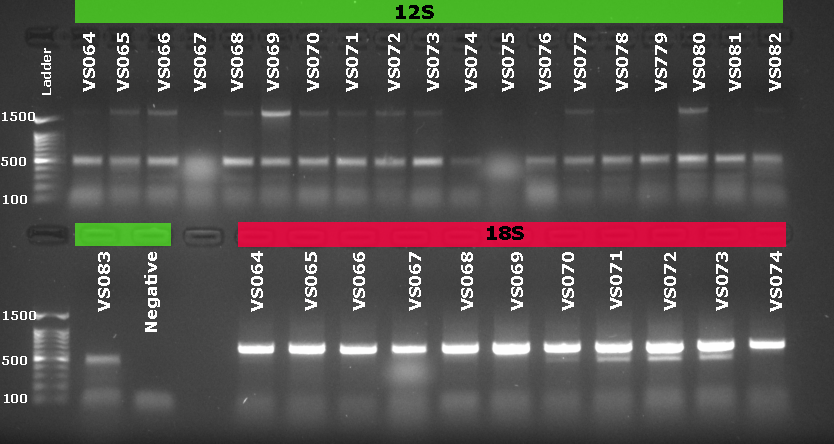
\includegraphics[scale = 1]{Images/12S_gel.pdf}
	\caption{12S and 18S PCR products visualised on 1\% agarose gel. Note the double bands in many of the 12S products; at the 500 and 1500 base pair mark.}
	\label{fig:12Sgel}
\end{figure}

\begin{figure}[H]
	\centering
	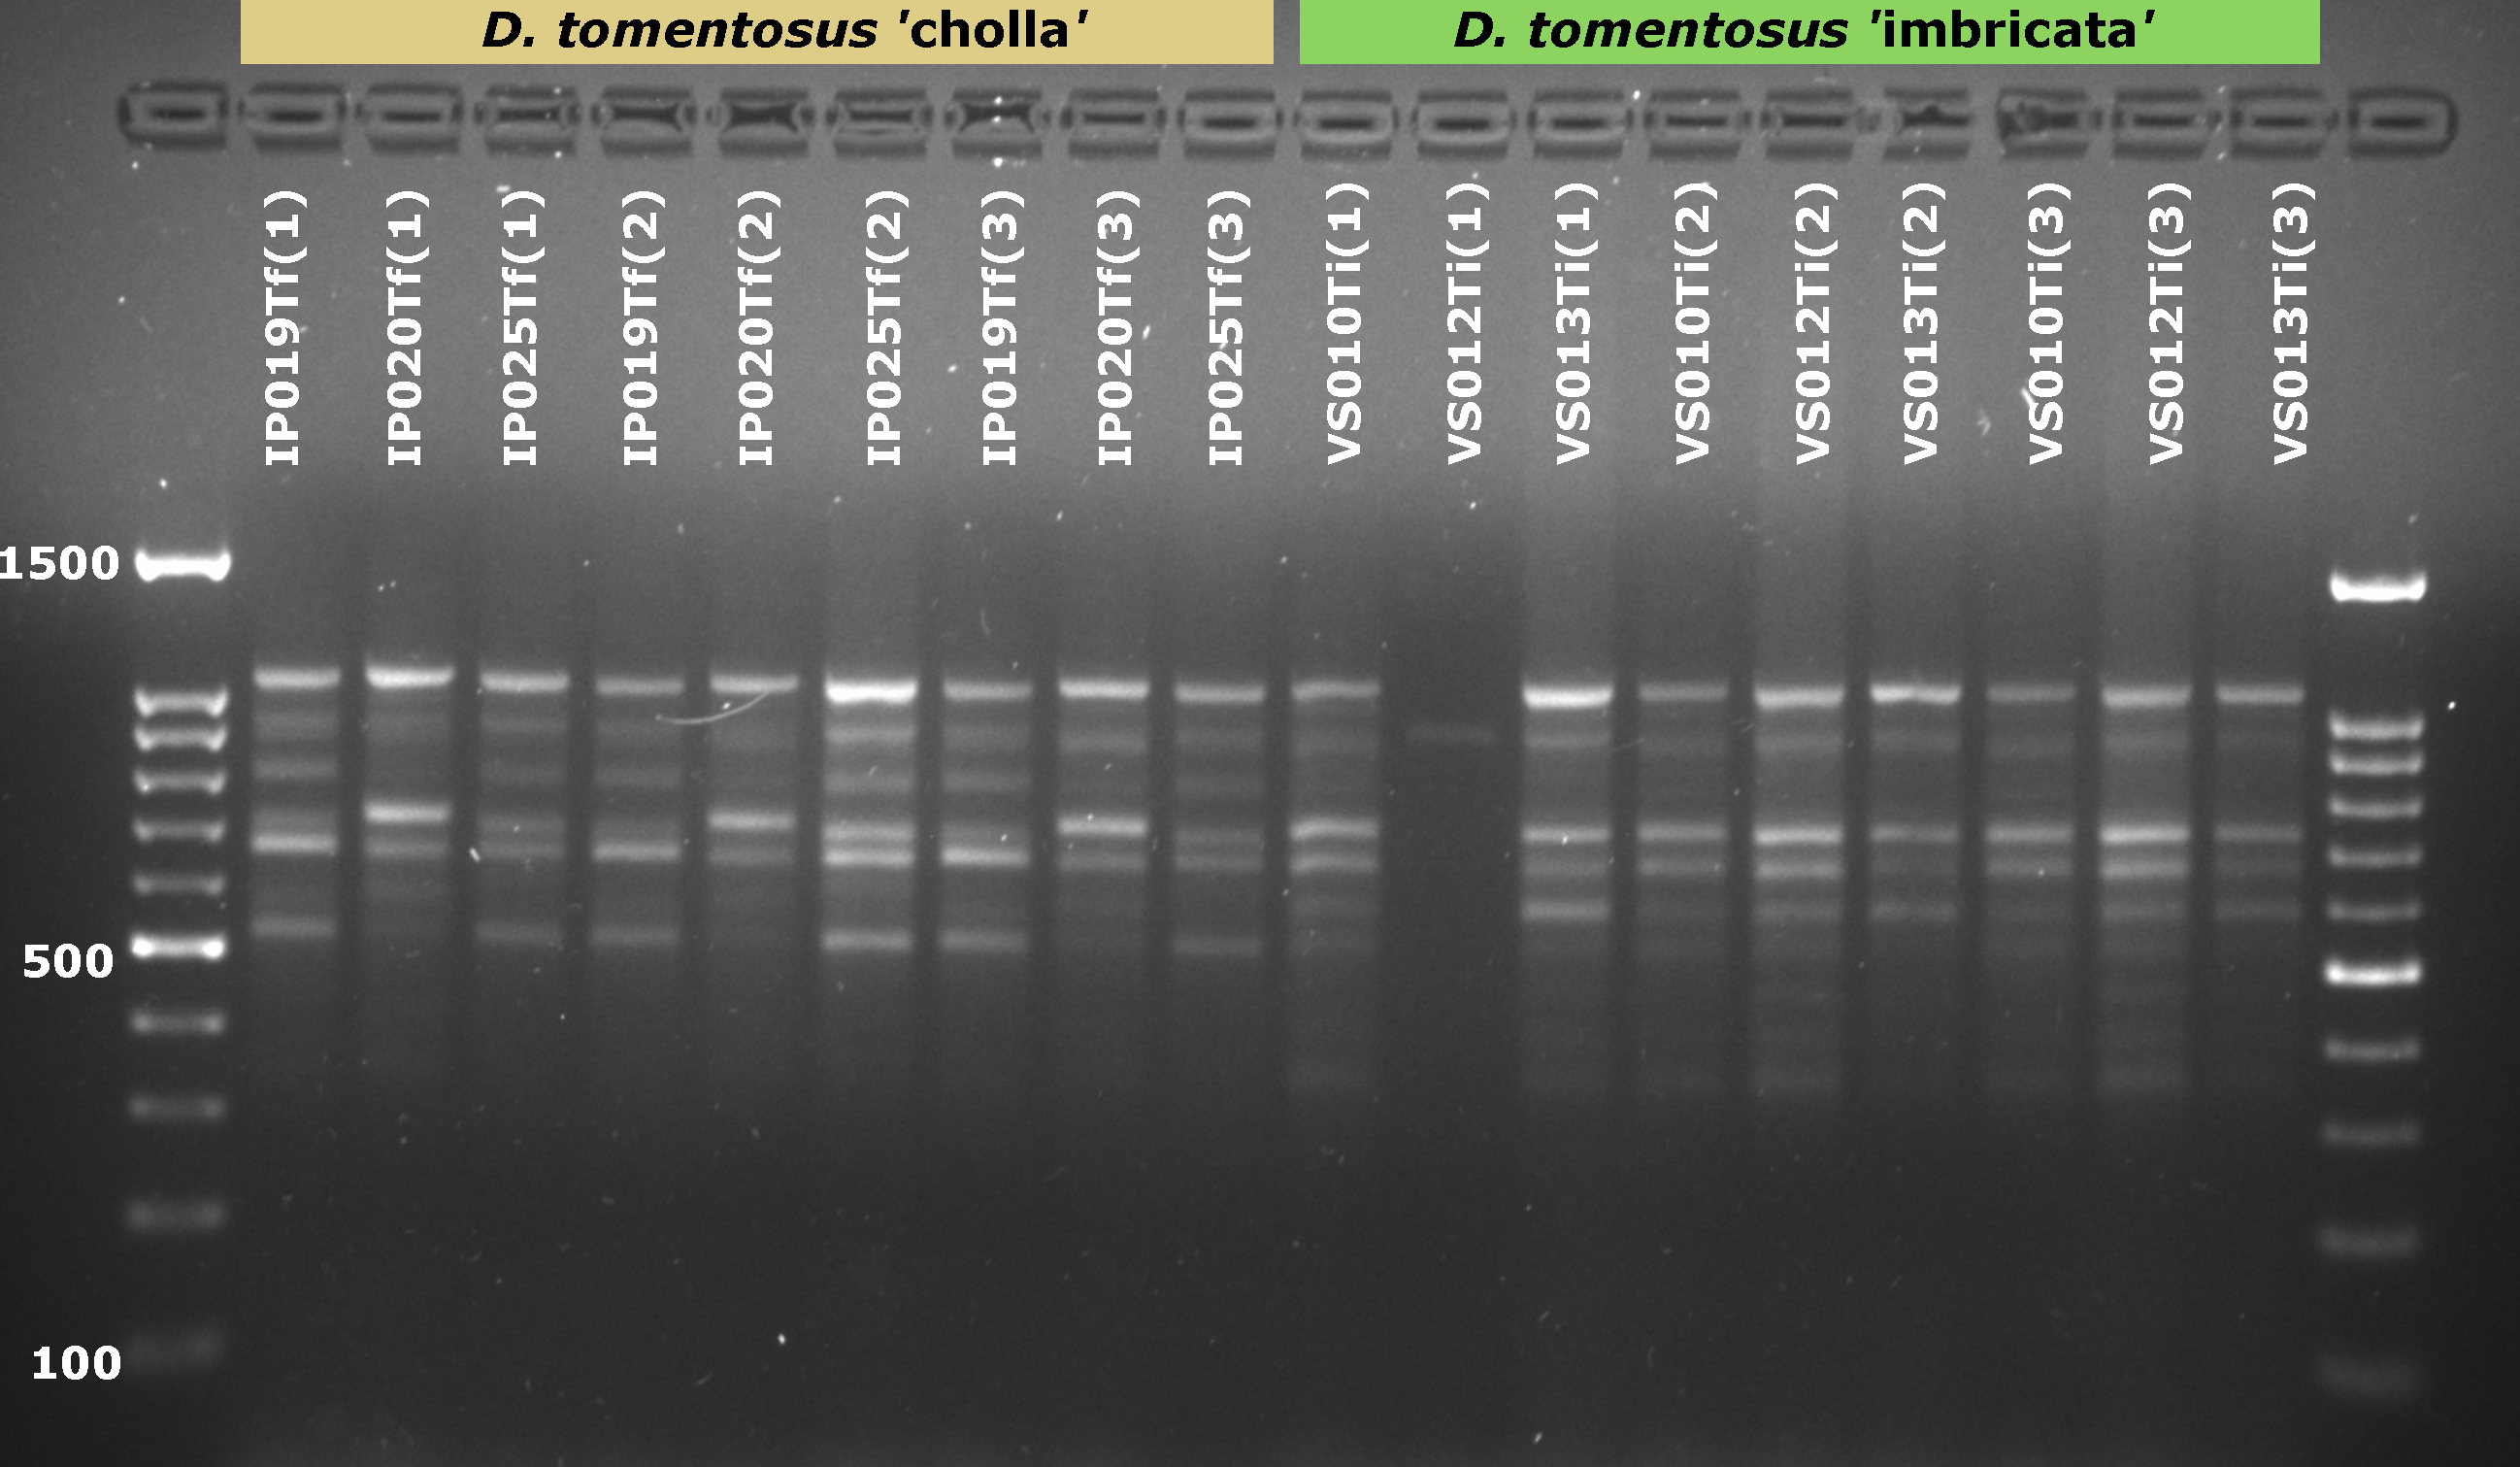
\includegraphics[scale = 0.3]{Images/ISSR_gel_T.pdf}
	\caption{ISSR banding pattern on a 1.5\% agarose gel for the two \textit{D. tomentosus} lineages (`cholla' and `imbricata'), run as a preliminary test before fragment analysis. Ladders are on the far left and right, marked at 100, 500 and 1500 base pair sizes.}
	\label{fig:issrGel}
\end{figure}

\begin{landscape}
{\scriptsize %
\renewcommand{\arraystretch}{0.5}
\begin{longtable}{@{}lllllp{2.7cm}p{2.2cm}p{5cm}p{4cm}@{}}
\caption{Genbank accession numbers for 12S, 18S and COI genetic sequences; with the extraction sample ID, species, lineage, locality and host plant information. CT Bot. Gard. = Cape Town Botanical Gardens, EC = Eastern Cape, KNP = Kruger National Park, MRF = Mass Rearing Facility. Black dots indicate samples collected in the native range in 2017.} \label{appendix:sequenceInfo} \\
\toprule
\textbf{12S} & \textbf{18S} & \textbf{COI DTOMf} & \textbf{COI PcoF1} & \textbf{Extraction ID} & \textbf{Species} & \textbf{Lineage} & \textbf{Locality} & \textbf{Host plant} \\ \midrule
MN220012 &  &  &  & VS021Au & \textit{D. austrinus} &  & South Africa: Uitenhage & \textit{Opuntia aurantiaca} \\
MN220013 & MN310065 &  &  & IP001Au & \textit{D. austrinus} &  & South Africa: Uitenhage & \textit{Opuntia aurantiaca} \\
MN220014 & MN310073 &  &  & VS001Au & \textit{D. austrinus} &  & South Africa: Uitenhage & \textit{Opuntia aurantiaca} \\
MN220038 & MN310132 &  &  & VS022Au & \textit{D. austrinus} &  & South Africa: Uitenhage & \textit{Opuntia aurantiaca} \\
MN220079 &  &  &  & VS089Au & \textit{D. austrinus} &  & South Africa: Uitenhage & \textit{Opuntia aurantiaca} \\
MN220091 & MN310131 &  &  & VS090Au & \textit{D. austrinus} &  & South Africa: Uitenhage & \textit{Opuntia aurantiaca} \\
MN220130 & MN310178 &  &  & Au4 & \textit{D. austrinus} &  & Australia: Queensland & \textit{Opuntia aurantiaca} \\
MN220131 & MN310179 &  &  & Au3 & \textit{D. austrinus} &  & Australia: Queensland & \textit{Opuntia aurantiaca} \\
MN220132 & MN310149 &  &  & Au1 & \textit{D. austrinus} &  & Australia: Queensland & \textit{Opuntia aurantiaca} \\
 & MN310069 &  &  & IP021Au & \textit{D. austrinus} &  & South Africa: Uitenhage & \textit{Opuntia aurantiaca} \\
 & MN310130 &  &  & VS091Au & \textit{D. austrinus} &  & South Africa: Uitenhage & \textit{Opuntia aurantiaca} \\
MN220010 &  &  &  & VS020C & \textit{D. ceylonicus} &  & South Africa: Uitenhage & \textit{Opuntia monacantha} \\
MN220011 & MN310074 &  &  & VS002C & \textit{D. ceylonicus} &  & South Africa: Uitenhage & \textit{Opuntia monacantha} \\
MN220037 & MN310134 &  &  & VS019C & \textit{D. ceylonicus} &  & South Africa: Uitenhage & \textit{Opuntia monacantha} \\
MN220039 & MN310133 &  &  & VS021C & \textit{D. ceylonicus} &  & South Africa: Uitenhage & \textit{Opuntia monacantha} \\
MN220122 & MN310173 &  &  & cey4 & \textit{D. ceylonicus} &  & Australia: Queensland & \textit{Opuntia monacantha} \\
MN220123 & MN310152 &  &  & cey3 & \textit{D. ceylonicus} &  & Australia: Queensland & \textit{Opuntia monacantha} \\
MN220124 & MN310160 &  &  & cey2 & \textit{D. ceylonicus} &  & Australia: Queensland & \textit{Opuntia monacantha} \\
 & MN310070 &  &  & IP022C & \textit{D. ceylonicus} &  & South Africa: Uitenhage & \textit{Opuntia monacantha} \\
 & MN310081 &  &  & VS020C & \textit{D. ceylonicus} &  & South Africa: Uitenhage & \textit{Opuntia monacantha} \\
 & MN310174 &  &  & cey1 & \textit{D. ceylonicus} &  & Australia: Queensland & \textit{Opuntia monacantha} \\
 & MN310037 &  & MN372226 & CSW001H & \textit{D. confertus} &  & Namibia, Windhoek & \textit{Harrisia sp.} \\
 & MN310038 &  & MN372227 & CSW002H & \textit{D. confertus} &  & Namibia, Windhoek & \textit{Harrisia sp.} \\
MN220015 & MN310099 &  & MN372274 & VS100Con\_s & \textit{D. confusus} &  & USA: Arizona, Tucson \textbullet & \textit{Opuntia santa-rita} \\
MN220016 & MN310100 &  &  & VS101Con\_e & \textit{D. confusus} &  & USA: Arizona, Tucson  & \textit{Opuntia engelmannii} \\
MN220017 & MN310101 &  &  & VS102Con\_e & \textit{D. confusus} &  & USA: Arizona, Tucson  & \textit{Opuntia engelmannii} \\
MN220018 & MN310102 &  &  & VS103Con\_e & \textit{D. confusus} &  & USA: Arizona, Tucson  & \textit{Opuntia engelmannii} \\
MN220019 & MN310103 &  &  & VS104Con\_e & \textit{D. confusus} &  & USA: Arizona, Tucson  & \textit{Opuntia engelmannii} \\
MN220029 &  &  & MN372263 & VS035O.4PM  & \textit{D. confusus} &  & USA: Arizona, Four Peaks Mt. \textbullet & \textit{Opuntia engelmannii} \\
MN220030 &  &  & MN372264 & VS036O.4PM  & \textit{D. confusus} &  & USA: Arizona, Four Peaks Mt. \textbullet & \textit{Opuntia engelmannii} \\
MN220031 & MN310091 &  & MN372265 & VS037O.4PM  & \textit{D. confusus} &  & USA: Arizona, Four Peaks Mt. \textbullet & \textit{Opuntia engelmannii} \\
MN220032 & MN310092 &  & MN372266 & VS038O.lc  & \textit{D. confusus} &  & USA: New Mexico, Las Cruces \textbullet & \textit{Opuntia engelmannii} \\
MN220033 & MN310093 &  & MN372267 & VS039O.lc  & \textit{D. confusus} &  & USA: New Mexico, Las Cruces \textbullet & \textit{Opuntia engelmannii} \\
MN220034 & MN310094 &  & MN372268 & VS040O.lc  & \textit{D. confusus} &  & USA: New Mexico, Las Cruces \textbullet & \textit{Opuntia engelmannii} \\
MN220054 & MN310054 &  & MN372240 & VS072u & \textit{D. confusus} &  & USA: Texas, Laredo \textbullet & \textit{Opuntia engelmannii} \\
MN220055 & MN310055 &  & MN372241 & VS073u & \textit{D. confusus} &  & USA: Texas, Laredo \textbullet & \textit{Opuntia engelmannii} \\
MN220056 & MN310056 &  & MN372242 & VS074u & \textit{D. confusus} &  & USA: Texas, Laredo \textbullet & \textit{Opuntia engelmannii} \\
MN220059 & MN310060 &  & MN372246 & VS078u & \textit{D. confusus} &  & USA: Arizona, Tucson \textbullet & \textit{Opuntia engelmannii} \\
MN220060 & MN310063 &  & MN372249 & VS081u & \textit{D. confusus} &  & USA: New Mexico, Las Cruces \textbullet & \textit{Opuntia engelmannii} \\
MN220063 & MN310061 &  & MN372247 & VS079u & \textit{D. confusus} &  & USA: Arizona, Tucson \textbullet & \textit{Opuntia engelmannii} \\
MN220064 & MN310062 &  & MN372248 & VS080u & \textit{D. confusus} &  & USA: New Mexico, Las Cruces \textbullet & \textit{Opuntia engelmannii} \\
 & MN310057 &  & MN372243 & VS075u & \textit{D. confusus} &  & USA: Texas, Laredo \textbullet & \textit{Opuntia engelmannii} \\
MN219994 & MN310078 &  &  & VS015Ofi & \textit{D. opuntiae} & ficus & South Africa: Uitenhage & \textit{Opuntia ficus-indica} \\
MN219995 & MN310079 &  & MN372255 & VS016Ofi & \textit{D. opuntiae} & ficus & South Africa: Uitenhage & \textit{Opuntia ficus-indica} \\
MN219996 & MN310080 &  & MN372256 & VS017Ofi & \textit{D. opuntiae} & ficus & South Africa: Uitenhage & \textit{Opuntia ficus-indica} \\
MN219997 & MN310095 &  & MN372269 & VS044Ofi & \textit{D. opuntiae} & ficus & Namibia: Auros farm & \textit{Opuntia ficus-indica} \\
MN219998 & MN310096 &  & MN372271 & VS046Ofi & \textit{D. opuntiae} & ficus & Namibia: Auros farm & \textit{Opuntia ficus-indica} \\
MN219999 & MN310142 &  & MN372270 & VS045Ofi & \textit{D. opuntiae} & ficus & Namibia: Auros farm & \textit{Opuntia ficus-indica} \\
MN220005 & MN310066 &  &  & IP003Os & \textit{D. opuntiae} &  & South Africa: Uitenhage, MRF & \textit{Opuntia ficus-indica} \\
MN220006 & MN310098 &  & MN372273 & VS054Os & \textit{D. opuntiae} & ficus & Namibia: Auros farm & \textit{Opuntia stricta} \\
MN220007 & MN310139 &  &  & VS055Os & \textit{D. opuntiae} & ficus & Namibia: Auros farm & \textit{Opuntia stricta} \\
MN220008 & MN310097 &  & MN372272 & VS053Os & \textit{D. opuntiae} & ficus & Namibia: Auros farm & \textit{Opuntia stricta} \\
MN220009 & MN310075 &  & MN372252 & VS004Os & \textit{D. opuntiae} &  & South Africa: Uitenhage, MRF & \textit{Opuntia ficus-indica} \\
MN220020 & MN310082 &  & MN372257 & VS026O.flag & \textit{D. opuntiae} &  & USA: Arizona, Flagstaff \textbullet & \textit{Opuntia engelmannii} \\
MN220021 & MN310083 &  & MN372258 & VS027O.flag & \textit{D. opuntiae} &  & USA: Arizona, Flagstaff \textbullet & \textit{Opuntia engelmannii} \\
MN220022 & MN310084 &  &  & VS028O.flag & \textit{D. opuntiae} &  & USA: Arizona, Flagstaff \textbullet & \textit{Opuntia engelmannii} \\
MN220023 & MN310085 &  &  & VS029O.tuc & \textit{D. opuntiae} &  & USA: Arizona, Tucson \textbullet & \textit{Opuntia engelmannii} \\
MN220024 & MN310086 &  & MN372259 & VS030O.tuc & \textit{D. opuntiae} &  & USA: Arizona, Tucson \textbullet & \textit{Opuntia engelmannii} \\
MN220025 & MN310087 &  & MN372260 & VS031O.tuc & \textit{D. opuntiae} &  & USA: Arizona, Tucson \textbullet & \textit{Opuntia engelmannii} \\
MN220026 & MN310088 &  & MN372261 & VS032O.sed & \textit{D. opuntiae} &  & USA: Arizona, Sedona \textbullet & \textit{Opuntia engelmannii} \\
MN220027 & MN310089 &  &  & VS033O.sed & \textit{D. opuntiae} &  & USA: Arizona, Sedona \textbullet & \textit{Opuntia engelmannii} \\
MN220028 & MN310090 &  & MN372262 & VS034O.sed & \textit{D. opuntiae} &  & USA: Arizona, Sedona \textbullet & \textit{Opuntia engelmannii} \\
MN220035 & MN310039 &  & MN372228 & CSW003E & \textit{D. opuntiae} & ficus & Namibia, Windhoek & \textit{Opuntia engelmannii} \\
MN220036 & MN310040 &  &  & CSW004E & \textit{D. opuntiae} & ficus & Namibia, Windhoek & \textit{Opuntia engelmannii} \\
MN220043 & MN310041 &  & MN372229 & VS059Os & \textit{D. opuntiae} &  & South Africa: Uitenhage, MRF & \textit{Opuntia ficus-indica} \\
MN220044 & MN310042 &  & MN372230 & VS060Os & \textit{D. opuntiae} &  & South Africa: Uitenhage, MRF & \textit{Opuntia ficus-indica} \\
MN220045 & MN310043 &  & MN372231 & VS061Os & \textit{D. opuntiae} &  & South Africa: Uitenhage, MRF & \textit{Opuntia ficus-indica} \\
MN220046 & MN310044 &  & MN372232 & VS062Os & \textit{D. opuntiae} &  & South Africa: Uitenhage, MRF & \textit{Opuntia ficus-indica} \\
MN220047 & MN310045 &  & MN372233 & VS063Os & \textit{D. opuntiae} &  & South Africa: Uitenhage, MRF & \textit{Opuntia ficus-indica} \\
MN220048 & MN310046 &  & MN372234 & VS064u & \textit{D. opuntiae} &  & USA: Texas, Moor Airbase \textbullet & \textit{Opuntia engelmannii} \\
MN220049 & MN310047 &  & MN372235 & VS065u & \textit{D. opuntiae} &  & USA: Texas, Moor Airbase \textbullet & \textit{Opuntia engelmannii} \\
MN220050 & MN310048 &  & MN372236 & VS066u & \textit{D. opuntiae} &  & USA: Texas, Port Isabel \textbullet & \textit{Opuntia engelmannii} \\
MN220051 & MN310050 &  & MN372238 & VS068u & \textit{D. opuntiae} &  & USA: Texas, Laredo \textbullet & \textit{Opuntia engelmannii} \\
MN220052 & MN310051 &  &  & VS069u & \textit{D. opuntiae} &  & USA: Texas, Laredo \textbullet & \textit{Opuntia engelmannii} \\
MN220053 & MN310053 &  & MN372239 & VS071u & \textit{D. opuntiae} &  & USA: Texas, Webb \textbullet & \textit{Opuntia engelmannii} \\
MN220057 & MN310058 &  & MN372244 & VS076u & \textit{D. opuntiae} &  & USA: California, Rincon \textbullet & \textit{Opuntia engelmannii} \\
MN220058 & MN310059 &  & MN372245 & VS077u & \textit{D. opuntiae} &  & USA: California, Rincon \textbullet & \textit{Opuntia engelmannii} \\
MN220061 &  &  &  & VS083u & \textit{D. opuntiae} &  & USA: Texas, Pecos County \textbullet & \textit{Opuntia engelmannii} \\
MN220062 & MN310052 &  &  & VS070u & \textit{D. opuntiae} &  & USA: Texas, Webb \textbullet & \textit{Opuntia engelmannii} \\
MN220065 & MN310104 &  &  & VS086uOE & \textit{D. opuntiae} & ficus & South Africa: Cookhouse, EC & \textit{Opuntia engelmannii} \\
MN220066 & MN310116 &  &  & VS087uOE & \textit{D. opuntiae} & ficus & South Africa: Cookhouse, EC & \textit{Opuntia engelmannii} \\
MN220067 & MN310115 &  &  & VS088uOE & \textit{D. opuntiae} & ficus & South Africa: Cookhouse, EC & \textit{Opuntia engelmannii} \\
MN220074 & MN310107 &  &  & VS106V & \textit{D. opuntiae} & ficus & South Africa: EC & \textit{Opuntia engelmannii} \\
MN220075 & MN310106 &  &  & VS107V & \textit{D. opuntiae} & ficus & South Africa: EC & \textit{Opuntia engelmannii} \\
MN220076 & MN310105 &  &  & VS108V & \textit{D. opuntiae} & ficus & South Africa: EC & \textit{Opuntia engelmannii} \\
MN220077 & MN310125 &  &  & P2S4 & \textit{D. opuntiae} & stricta & South Africa: KNP & \textit{Opuntia stricta} \\
MN220078 & MN310122 &  & MN372278 & P3S2 & \textit{D. opuntiae} & stricta & South Africa: KNP & \textit{Opuntia stricta} \\
MN220080 & MN310145 &  &  & BCCS1 & \textit{D. opuntiae} & stricta & South Africa: KNP, Skukuza & \textit{Opuntia stricta} \\
MN220081 & MN310127 &  & MN372275 & P1S4 & \textit{D. opuntiae} & stricta & South Africa: KNP & \textit{Opuntia stricta} \\
MN220082 &  &  &  & VS054Os & \textit{D. opuntiae} & ficus & South Africa: Namibia & \textit{Opuntia stricta} \\
MN220083 & MN310123 &  &  & P3S1 & \textit{D. opuntiae} & stricta & South Africa: KNP & \textit{Opuntia stricta} \\
MN220084 & MN310128 &  & MN372279 & P1S3 & \textit{D. opuntiae} & stricta & South Africa: KNP & \textit{Opuntia stricta} \\
MN220085 & MN310119 &  & MN372277 & VS151H & \textit{D. opuntiae} & stricta & South Africa & \textit{Opuntia stricta} \\
MN220086 & MN310143 &  & MN372280 & BCCS4 & \textit{D. opuntiae} & stricta & South Africa: KNP, Skukuza & \textit{Opuntia stricta} \\
MN220087 & MN310124 &  &  & P2S5 & \textit{D. opuntiae} & stricta & South Africa: KNP & \textit{Opuntia stricta} \\
MN220088 & MN310129 &  &  & P1S1 & \textit{D. opuntiae} & stricta & South Africa: KNP & \textit{Opuntia stricta} \\
MN220089 & MN310121 &  &  & VS149K & \textit{D. opuntiae} & stricta & South Africa & \textit{Opuntia stricta} \\
MN220090 & MN310144 &  &  & BCCS2 & \textit{D. opuntiae} & stricta & South Africa: KNP, Skukuza & \textit{Opuntia stricta} \\
MN220092 &  &  &  & VS146K & \textit{D. opuntiae} & stricta & South Africa & \textit{Opuntia stricta} \\
MN220093 & MN310126 &  &  & P2S2 & \textit{D. opuntiae} & stricta & South Africa: KNP & \textit{Opuntia stricta} \\
MN220094 & MN310118 &  & MN372276 & VS152H & \textit{D. opuntiae} & stricta & South Africa & \textit{Opuntia stricta} \\
MN220095 & MN310117 &  &  & VS154H & \textit{D. opuntiae} & stricta & South Africa & \textit{Opuntia stricta} \\
MN220096 &  &  &  & Ah2 & \textit{D. opuntiae} & stricta & Saudi Arabia: Jazan, Alaredah & \textit{Opuntia stricta} \\
MN220097 & MN310163 &  &  & op4 & \textit{D. opuntiae} &  & Australia: Queensland & \textit{Opuntia stricta} \\
MN220098 & MN310147 &  &  & op3 & \textit{D. opuntiae} &  & Australia: Queensland & \textit{Opuntia stricta} \\
MN220099 & MN310162 &  &  & op1 & \textit{D. opuntiae} &  & Australia: Queensland & \textit{Opuntia stricta} \\
MN220100 &  &  &  & JC3 & \textit{D. opuntiae} & stricta & Saudi Arabia: Jazan, Jazan City & \textit{Opuntia stricta} \\
MN220101 &  &  &  & JC2 & \textit{D. opuntiae} & stricta & Saudi Arabia: Jazan, Jazan City & \textit{Opuntia stricta} \\
MN220106 &  &  &  & H4 & \textit{D. opuntiae} & stricta & Saudi Arabia: Jazan, Hurob & \textit{Opuntia stricta} \\
MN220107 &  &  &  & H1 & \textit{D. opuntiae} & stricta & Saudi Arabia: Jazan, Hurob & \textit{Opuntia stricta} \\
MN220108 & MN310155 &  &  & eng1 & \textit{D. opuntiae} &  & Australia: Queensland & \textit{Opuntia engelmannii} \\
MN220111 & MN310166 &  &  & eng4 & \textit{D. opuntiae} &  & Australia: Queensland & \textit{Opuntia engelmannii} \\
MN220133 &  &  &  & AL3 & \textit{D. opuntiae} & stricta & Saudi Arabia: Jazan, Aldyer & \textit{Opuntia stricta} \\
MN220134 &  &  &  & AL2 & \textit{D. opuntiae} & stricta & Saudi Arabia: Jazan, Aldyer & \textit{Opuntia stricta} \\
MN220135 &  &  &  & Ah4 & \textit{D. opuntiae} & stricta & Saudi Arabia: Jazan, Alaredah & \textit{Opuntia stricta} \\
 & MN310049 &  & MN372237 & VS067u & \textit{D. opuntiae} &  & USA: Texas, Port Isabel & \textit{Opuntia engelmannii} \\
 & MN310064 &  & MN372250 & VS082u & \textit{D. opuntiae} &  & USA: Texas, Pecos County & \textit{Opuntia engelmannii} \\
 & MN310071 &  &  & IP024Os & \textit{D. opuntiae} &  & South Africa: Uitenhage, MRF & \textit{Opuntia ficus-indica} \\
 & MN310120 &  &  & VS150K & \textit{D. opuntiae} & stricta & South Africa & \textit{Opuntia stricta} \\
 & MN310140 &  &  & CVS262 & \textit{D. opuntiae} & ficus & South Africa: Uitenhage & \textit{Opuntia stricta} \\
 & MN310141 &  &  & CVS261 & \textit{D. opuntiae} & ficus & South Africa: Uitenhage & \textit{Opuntia stricta} \\
 & MN310167 &  &  & eng3 & \textit{D. opuntiae} &  & Australia: Queensland & \textit{Opuntia engelmannii} \\
 &  &  & MN372253 & VS008Ofi & \textit{D. opuntiae} & ficus & South Africa: Uitenhage & \textit{Opuntia ficus-indica} \\
MN220000 & MN310137 &  &  & VS014Ti & \textit{D. tomentosus} & imbricata & South Africa: Uitenhage & \textit{Cylindropuntia imbricata} \\
MN220001 & MN310077 &  &  & VS013Ti & \textit{D. tomentosus} & imbricata & South Africa: Uitenhage & \textit{Cylindropuntia imbricata} \\
MN220002 & MN310076 &  & MN372254 & VS012Ti & \textit{D. tomentosus} & imbricata & South Africa: Uitenhage & \textit{Cylindropuntia imbricata} \\
MN220102 & MN310164 &  &  & imb4 & \textit{D. tomentosus} & imbricata & Australia: Queensland & \textit{Cylindropuntia imbricata} \\
MN220103 & MN310165 &  &  & imb3 & \textit{D. tomentosus} & imbricata & Australia: Queensland & \textit{Cylindropuntia imbricata} \\
MN220104 & MN310156 &  &  & imb2 & \textit{D. tomentosus} & imbricata & Australia: Queensland & \textit{Cylindropuntia imbricata} \\
MN220105 & MN310148 &  &  & imb1 & \textit{D. tomentosus} & imbricata & Australia: Queensland & \textit{Cylindropuntia imbricata} \\
 &  &  & MN372299 & IP005Ti & \textit{D. tomentosus} & imbricata & South Africa: Uitenhage & \textit{Cylindropuntia imbricata} \\
MN220041 & MN310138 &  &  & VS010Ti & \textit{D. tomentosus} & imbricata & South Africa: Uitenhage & \textit{Cylindropuntia imbricata} \\
MN220042 & MN310136 &  &  & IP016Ti & \textit{D. tomentosus} & imbricata & South Africa: Uitenhage & \textit{Cylindropuntia imbricata} \\
MN220003 & MN310072 &  & MN372251 & IP025Tf & \textit{D. tomentosus} & cholla & South Africa: CT Bot. Gard. & \textit{C. fulgida var. mamm.} \\
MN220004 & MN310135 &  &  & VS005Tf & \textit{D. tomentosus} & cholla & South Africa: CT Bot. Gard. & \textit{C. fulgida var. mamm.} \\
MN220040 & MN310068 & MN372298 &  & IP019Tf & \textit{D. tomentosus} & cholla & South Africa: CT Bot. Gard. & \textit{C. fulgida var. mamm.} \\
MN220068 & MN310114 &  &  & VS098Tf & \textit{D. tomentosus} & cholla & South Africa: CT Bot. Gard. & \textit{C. fulgida var. mamm.} \\
MN220069 & MN310113 &  &  & VS099Tf & \textit{D. tomentosus} & cholla & South Africa: CT Bot. Gard. & \textit{C. fulgida var. mamm.} \\
MN220109 &  &  &  & Ekh6 & \textit{D. tomentosus} & cholla & South Africa: Jansenville, EC & \textit{Cylindropuntia fulgida} \\
MN220110 &  &  &  & EKh5 & \textit{D. tomentosus} & cholla & South Africa: Jansenville, EC & \textit{Cylindropuntia fulgida} \\
MN220112 &  &  &  & Ekh4 & \textit{D. tomentosus} & cholla & South Africa: Jansenville, EC & \textit{Cylindropuntia fulgida} \\
MN220119 &  & MN372287 &  & chol4 & \textit{D. tomentosus} & cholla & Australia: Queensland & \textit{Cylindropuntia fulgida} \\
MN220120 & MN310153 & MN372288 &  & chol3 & \textit{D. tomentosus} & cholla & Australia: Queensland & \textit{Cylindropuntia fulgida} \\
MN220121 & MN310172 & MN372290 &  & chol1 & \textit{D. tomentosus} & cholla & Australia: Queensland & \textit{Cylindropuntia fulgida} \\
 & MN310161 & MN372289 &  & chol2 & \textit{D. tomentosus} & cholla & Australia: Queensland & \textit{C. fulgida var. mamm.} \\
 & MN310067 &  &  & IP005Tf & \textit{D. tomentosus} & cholla & South Africa: CT Bot. Gard. & \textit{C. fulgida var. mamm.} \\
MN220070 & MN310112 &  &  & VS101Tp & \textit{D. tomentosus} & californica & Australia: Queensland & \textit{Cylindropuntia pallida} \\
MN220071 & MN310111 &  &  & VS102Tp & \textit{D. tomentosus} & californica & Australia: Queensland & \textit{Cylindropuntia pallida} \\
MN220072 & MN310109 &  &  & VS104Tp & \textit{D. tomentosus} & californica & Australia: Queensland & \textit{Cylindropuntia pallida} \\
MN220073 & MN310108 &  &  & VS105Tp & \textit{D. tomentosus} & californica & Australia: Queensland & \textit{Cylindropuntia pallida} \\
MN220125 & MN310175 & MN372291 &  & Cal4 & \textit{D. tomentosus} & californica & Australia: Queensland & \textit{Cylindropuntia pallida} \\
MN220126 & MN310151 & MN372292 &  & Cal3 & \textit{D. tomentosus} & californica & Australia: Queensland & \textit{Cylindropuntia pallida} \\
MN220127 & MN310158 & MN372293 &  & Cal2 & \textit{D. tomentosus} & californica & Australia: Queensland & \textit{Cylindropuntia pallida} \\
MN220128 & MN310176 & MN372294 &  & Cal1 & \textit{D. tomentosus} & californica & Australia: Queensland & \textit{Cylindropuntia pallida} \\
 & MN310110 &  &  & VS103Tp & \textit{D. tomentosus} & californica & Australia: Queensland & \textit{Cylindropuntia pallida} \\
MN220113 & MN310146 & MN372281 &  & ech4 & \textit{D. tomentosus} & ech. x acanth. & Australia: Queensland & \textit{\begin{tabular}[c]{@{}l@{}}C. ech. x  C. acanth.\end{tabular}} \\
MN220114 & MN310168 & MN372282 &  & ech3 & \textit{D. tomentosus} & ech. x acanth. & Australia: Queensland & \textit{\begin{tabular}[c]{@{}l@{}}C. ech. x C. acanth.\end{tabular}} \\
MN220115 &  & MN372283 &  & ech2 & \textit{D. tomentosus} & ech. x acanth. & Australia: Queensland & \textit{\begin{tabular}[c]{@{}l@{}}C. ech. x C. acanth.\end{tabular}} \\
MN220118 & MN310169 & MN372284 &  & ech1 & \textit{D. tomentosus} & ech. x acanth. & Australia: Queensland & \textit{\begin{tabular}[c]{@{}l@{}}C. ech. x C. acanth.\end{tabular}} \\
MN220116 & MN310157 & MN372285 &  & cyl3 & \textit{D. tomentosus} & cylindropuntia & Australia: Queensland & \textit{Cylindropuntia sp.} \\
MN220117 & MN310170 & MN372286 &  & cyl2 & \textit{D. tomentosus} & cylindropuntia & Australia: Queensland & \textit{Cylindropuntia sp.} \\
 & MN310154 &  &  & cyl4 & \textit{D. tomentosus} & cylindropuntia & Australia: Queensland & \textit{Cylindropuntia sp.} \\
 & MN310171 &  &  & cyl1 & \textit{D. tomentosus} & cylindropuntia & Australia: Queensland & \textit{Cylindropuntia sp.} \\
MN220129 & MN310159 & MN372297 &  & Big2 & \textit{D. tomentosus} & bigelovii & Australia: Queensland & \textit{Cylindropuntia bigelovii} \\
 & MN310150 & MN372296 &  & Big3 & \textit{D. tomentosus} & bigelovii & Australia: Queensland & \textit{Cylindropuntia bigelovii} \\
 & MN310177 & MN372295 &  & Big5 & \textit{D. tomentosus} & bigelovii & Australia: Queensland & \textit{Cylindropuntia bigelovii} \\ \bottomrule
\end{longtable}
}%


\begin{table}[H]
\centering
\caption{Sample IDs for additional DNA extractions used for ISSR analyses.}
\label{appendix:issr_sample_table}
{\scriptsize %
\renewcommand{\arraystretch}{0.5}
\begin{tabular}{@{}lllll@{}}
\toprule
\textbf{Extraction ID} & \textbf{Species} & \textbf{Lineage} & \textbf{Locality} & \textbf{Host plant} \\ \midrule
VS121O.4PM & \textit{D. confusus} &  & USA: Arizona, Four Peaks Mt. & \textit{O. engelmannii} \\
VS124O.lc & \textit{D. confusus} &  & USA: New Mexico, Las Cruces & \textit{O. engelmannii} \\
VS136 & \textit{D. confusus} &  & USA: Texas, Laredo & \textit{O. engelmannii} \\
VS137 & \textit{D. confusus} &  & USA: Texas, Laredo & \textit{O. engelmannii} \\
VS138 & \textit{D. confusus} &  & USA: Texas, Laredo & \textit{O. engelmannii} \\
VS139 & \textit{D. confusus} &  & USA: Texas, Laredo & \textit{O. engelmannii} \\
VS141 & \textit{D. confusus} &  & USA: Arizona, Tucson & \textit{O. engelmannii} \\
VS142 & \textit{D. confusus} &  & USA: Arizona, Tucson & \textit{O. engelmannii} \\
VS143 & \textit{D. confusus} &  & USA: New Mexico, Las Cruces & \textit{O. engelmannii} \\
VS144 & \textit{D. confusus} &  & USA: New Mexico, Las Cruces & \textit{O. engelmannii} \\
VS110 & \textit{D. opuntiae} & `ficus' & South Africa: EC, Prieel, near Fort Beaufort & \textit{O. ficus-indica} \\
VS111 & \textit{D. opuntiae} & `ficus' & South Africa: EC, Prieel, near Fort Beaufort & \textit{O. ficus-indica} \\
VS112 & \textit{D. opuntiae} & `ficus' & South Africa: EC, Prieel, near Fort Beaufort & \textit{O. ficus-indica} \\
VS113 & \textit{D. opuntiae} & `ficus' & South Africa: EC, Prieel, near Fort Beaufort & \textit{O. engelmannii} \\
VS114 & \textit{D. opuntiae} & `ficus' & South Africa: EC, Prieel, near Fort Beaufort & \textit{O. engelmannii} \\
VS115 & \textit{D. opuntiae} & `ficus' & South Africa: EC, Prieel, near Fort Beaufort & \textit{O. engelmannii} \\
VS116 & \textit{D. opuntiae} & `ficus' & South Africa: EC, Kluklu farm, near Fort Beaufort & \textit{O. engelmannii} \\
VS117 & \textit{D. opuntiae} & `ficus' & South Africa: EC, Kluklu farm, near Fort Beaufort & \textit{O. engelmannii} \\
VS118 & \textit{D. opuntiae} & `ficus' & South Africa: EC, Kluklu farm, near Fort Beaufort & \textit{O. engelmannii} \\
VS119O.flag & \textit{D. opuntiae} &  & USA: Arizona, Flagstaff & \textit{O. engelmannii} \\
VS120O.flag & \textit{D. opuntiae} &  & USA: Arizona, Flagstaff & \textit{O. engelmannii} \\
VS126O.sed & \textit{D. opuntiae} &  & USA: Arizona, Sedona & \textit{O. engelmannii} \\
VS129 & \textit{D. opuntiae} &  & USA: Texas, Moor Airbase & \textit{O. engelmannii} \\
VS130 & \textit{D. opuntiae} &  & USA: Texas, Port Isabel & \textit{O. engelmannii} \\
VS131 & \textit{D. opuntiae} &  & USA: Texas, Port Isabel & \textit{O. engelmannii} \\
VS132 & \textit{D. opuntiae} &  & USA: Texas, Laredo & \textit{O. engelmannii} \\
VS133 & \textit{D. opuntiae} &  & USA: Texas, Laredo & \textit{O. engelmannii} \\
VS134 & \textit{D. opuntiae} &  & USA: Texas, Webb & \textit{O. engelmannii} \\
VS135 & \textit{D. opuntiae} &  & USA: Texas, Webb & \textit{O. engelmannii} \\
VS140 & \textit{D. opuntiae} &  & USA: California, Rincon & \textit{O. engelmannii} \\
VS145 & \textit{D. opuntiae} &  & USA: Texas, Pecos County & \textit{O. engelmannii} \\
VS092Ti & \textit{D. tomentosus} & `imbricata' & South Africa: Uitenhage MRF & \textit{C. imbricata} \\
VS093Ti & \textit{D. tomentosus} & `imbricata' & South Africa: Uitenhage MRF & \textit{C. imbricata} \\
VS100Tf & \textit{D. tomentosus} & `cholla' & South Africa: Uitenhage MRF & \textit{C. fulgida} var. \textit{mamillata} \\ \bottomrule
\end{tabular}
}%
\end{table}


\begin{table}[H]
\caption{Genbank sequences used to supplement the dataset for this project. PcoF1 \& LepR1 and DTOMf \& HCO2198 are both COI primers that amplify the same region of the COI gene.} \label{appendix:outgroups}
\centering
{\scriptsize %
\renewcommand{\arraystretch}{0.4}
\begin{tabular}{@{}lllll@{}} \\ \toprule
\multicolumn{4}{c}{\textbf{Genbank accession numbers}} & \multicolumn{1}{c}{\textbf{Organism}}  \\ \toprule
\multicolumn{1}{c}{\textbf{12S}} & \textbf{18S} & \textbf{PcoF1 \& LepR1} & \textbf{DTOMf \& HCO2198} &  \\ \bottomrule
HQ893819.1 & KY9276001 &  &  & \textit{Parasaissetia nigra} \\
HQ893810.1 & HQ8937881 &  &  & \textit{Ceroplastes sinensis} \\
HQ893818.1 & HQ8937931 & GU936953.1 &  & \textit{Coccus viridis} \\
KT199030.1 & KT199030.1 &  &  & \textit{Marchalina hellenica} \\
HQ893806.1 & KT199034.1 & KP692469.1 &  & \textit{Icerya purchasi} \\
KJ701959.1 & KJ7019951 &  &  & \textit{Dactylopius coccus} \\
KJ701960.1 & KJ7019941 &  &  & \textit{Dactylopius coccus} \\
KJ701961.1 & KJ7019931 &  &  & \textit{Dactylopius coccus} \\
KJ701962.1 & KJ7019921 &  &  & \textit{Dactylopius coccus} \\
KJ701963.1 & KJ7019911 &  &  & \textit{Dactylopius coccus} \\
 &  &  &  & \textit{Ceroplastes sp.} \\
 &  &  & GU228789.1 & \textit{Dactylopius opuntiae} \\
 &  &  & GU228788.1 & \textit{Dactylopius tomentosus 'Imbricata'} \\
 &  &  & GU228787.1 & \textit{Dactylopius tomentosus 'Imbricata'} \\
 &  &  & GU228786.1 & \textit{Dactylopius tomentosus 'RoseaP'} \\
 &  &  & GU228781.1 & \textit{Dactylopius tomentosus 'ChollaDH'} \\
 &  &  & GU228780.1 & \textit{Dactylopius tomentosus 'ChollaE'} \\
 &  &  & GU228779.1 & \textit{Dactylopius tomentosus 'ChollaD'} \\
 &  &  & GU228785.1 & \textit{Dactylopius tomentosus 'RoseaY'} \\
 &  &  & GU228784.1 & \textit{Dactylopius tomentosus 'Fulgida'} \\
 &  &  & GU228783.1 & \textit{Dactylopius tomentosus 'Mamillata'} \\
 &  &  & GU228782.1 & \textit{Dactylopius tomentosus 'Molesta'} \\
 &  &  & AB440069.2 & \textit{Coccus hesperidum} \\
 &  &  & AB440071.1 & \textit{Eulecanium kunoense} \\
 &  &  & AB440073.1 & \textit{Parthenolecanium pruinosum} \\
 &  &  & AB440072.2 & \textit{Pulvinaria psidii} \\ \bottomrule
\end{tabular}
}%
\end{table}

% Please add the following required packages to your document preamble:
% \usepackage{booktabs}
\begin{table}[H]
\caption{Rhodes University and Agricultural Research Council (ARC) accession numbers for \textit{Dactylopius} samples from the native range (USA), identified by Ian Millar in 2019. Representative sample IDs refer to those used in the gene phylogenies in this project. See Table \ref{appendix:sequenceInfo} for the full list of sequences.} \label{appendix:ianMillarIds}
\centering
{\scriptsize %
\renewcommand{\arraystretch}{0.4}
\begin{tabular}{@{}llll@{}}
\toprule
\textbf{\begin{tabular}[c]{@{}l@{}}Rhodes University \\ Accession Number\end{tabular}} & \textbf{\begin{tabular}[c]{@{}l@{}}ARC \\ Accession Number\end{tabular}} & \textbf{Identity} & \textbf{\begin{tabular}[c]{@{}l@{}}Representative \\ sample ID\end{tabular}} \\ \midrule
RH1283 & HC 7331 & \textit{D. confertus} & \multirow{3}{*}{CSW001H} \\
RH1284 & HC 7331 & \textit{D. confertus} &  \\
RH1285 & HC 7331 & \textit{D. confertus} &  \\
RH1286 & HC 7332 & \textit{D. confusus} & VS072u \\
RH1287 & HC 7333 & \textit{D. opuntiae} & VS083u \\
RH1288 & HC 7334 & \textit{D. opuntiae} & VS069u \\
RH1289 &  & \textit{D. confusus} & VS080u \\
RH1290 & HC 7335 & \textit{D. opuntiae} & VS064u \\
RH1291 & HC 7336 & \textit{D. opuntiae} & VS077u \\
RH1292 & HC 7337 & \textit{D. opuntiae} & VS083u \\
RH1293 & HC 7338 & \textit{D. confusus} & VS073u \\
RH1294 &  & \textit{D. confusus} & VS078u \\
RH1295 &  & \textit{D. opuntiae} & VS066u \\ \bottomrule
\end{tabular}
}%
\end{table}

\end{landscape}


\begin{landscape}
\label{sec:tcoffee}

\begin{figure}[H]
	\centering
	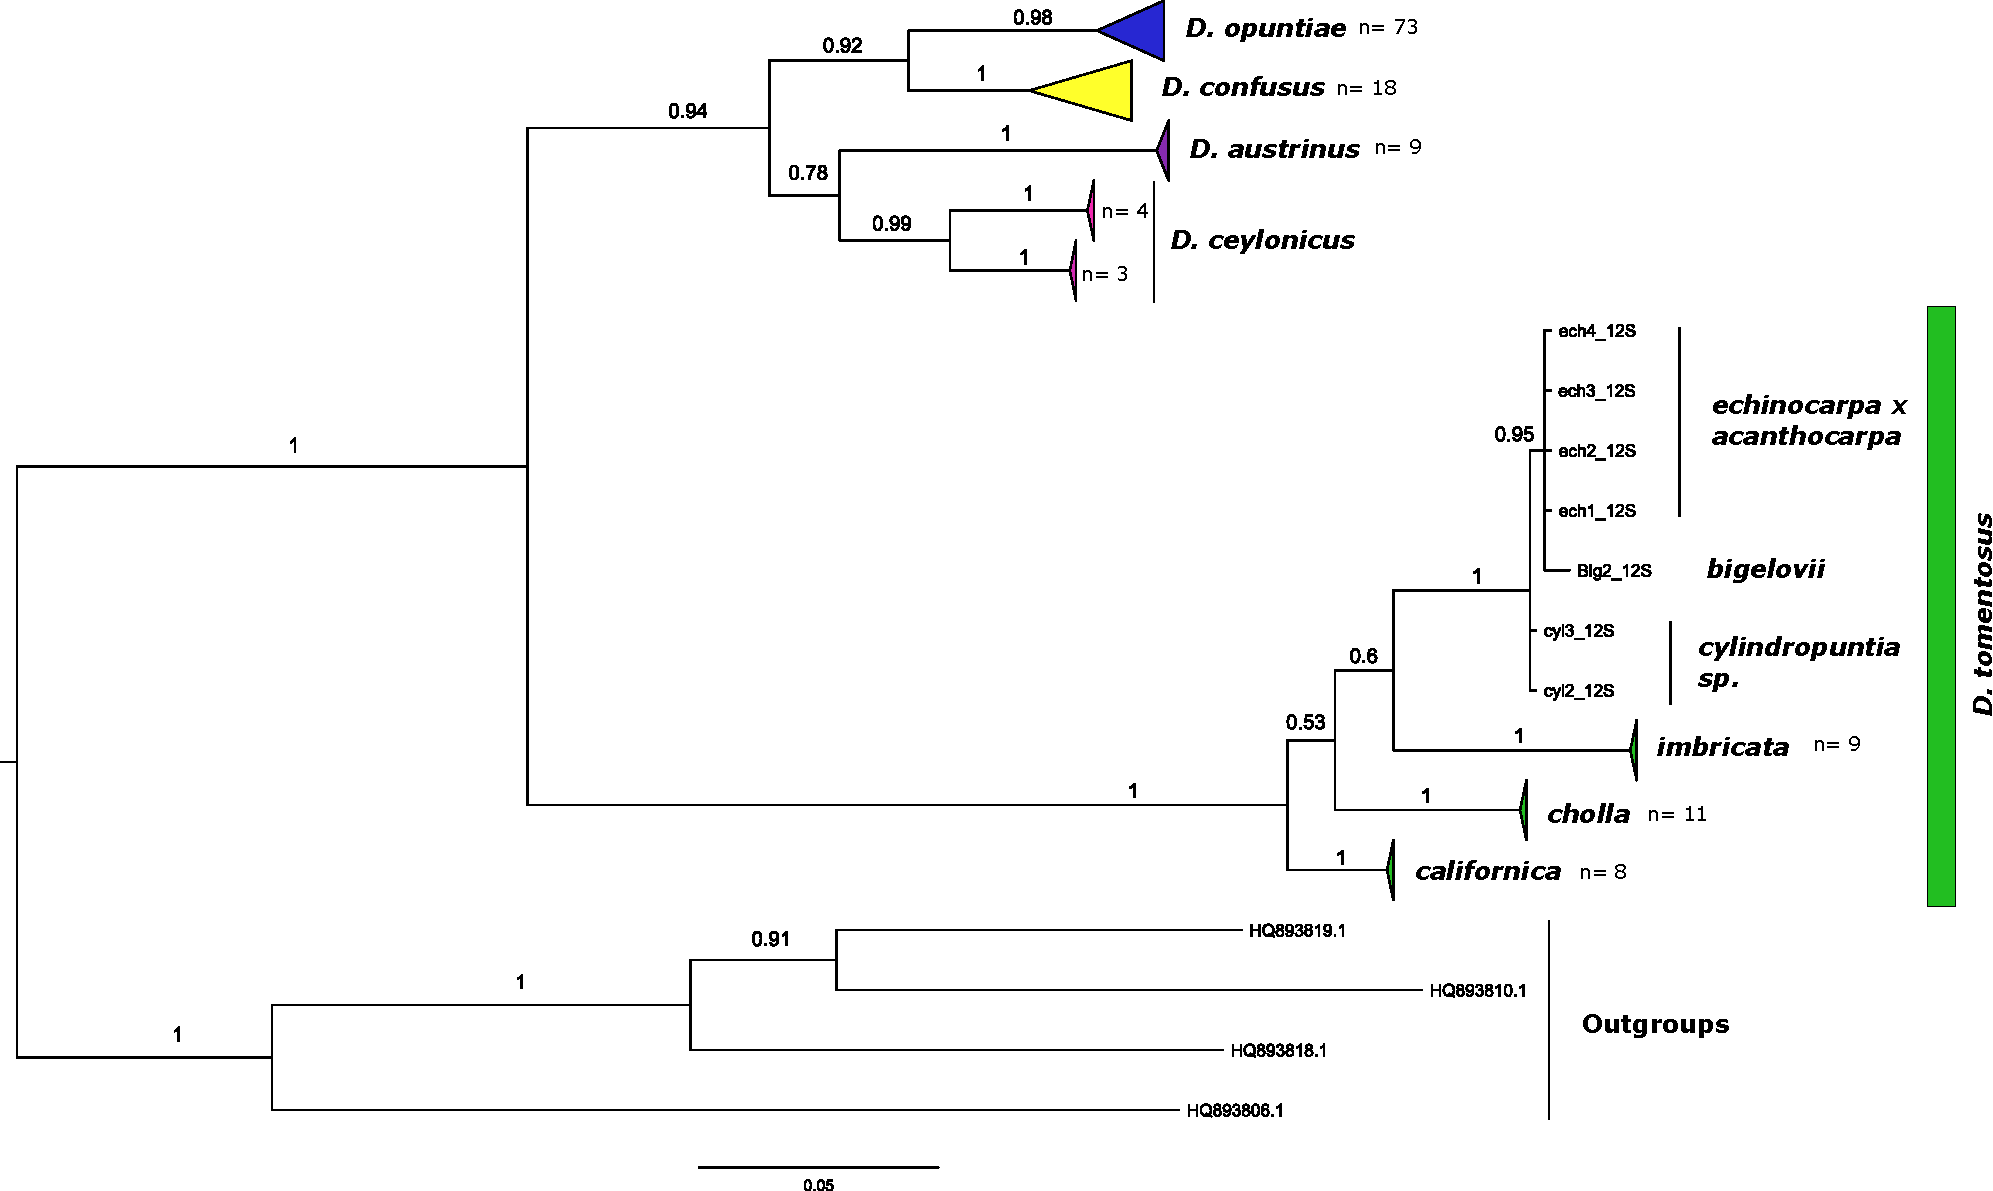
\includegraphics[scale =0.7]{Images/12S_rcoffee_collapsed_export.pdf}
	\caption{12S rRNA Bayesian phylogeny based on the alignment obtained from R-Coffee, which aligns RNA sequences according to their secondary structure. The HKY + I + G model was used, where shapepr = 0.9980, pinvarp = 0.1420 and tratiopr = 1.4096. State frequencies were 0.5155, 0.0897, 0.0282 and 0.3665. Major clades have been collapsed.}  
	\label{fig:12S_rcoffee}
\end{figure}

\end{landscape}

\section{Program settings and file formats}
\subsection{GeneMarker}
\label{appendix:genemarker_settings}

\begin{enumerate}
    \item Size standard set to `GS500LIZ' (Size editor $\rightarrow$ File $\rightarrow$ Import ABI Size Standard $\rightarrow$ select the desired size standard file) and Analysis Type to `AFLP'.
    \item The selected Raw Data Analysis settings were: Auto Range (frame), Saturation Repair, Baseline Subtraction, Pull-up Correction, Spike Removal and Local Southern.
    \item Allele Call settings were: Allele calls set to the `automatic'. Minimum Intensity for peak detection set at 50 RFU (relative fluorescence units) and Max Intensity left at the default (30000 RFU). This minimum intensity is recommended by \citet{arrigo2012automated} as a more permissive prior screening approach. \citet{prince2009} used an even lower threshold, set at 20 RFU. Peaks below the threshold are most likely due to the slippage of polymerase during the PCR elongation step, sometimes referred to as `taq stutter' \citep{DNAFragAnalysis, prince2009}. Plus-A Filter was left selected.
    \item `AFLP normalization' selected.
    \item The summary table was obtained by selecting `Report settings' followed by `Peak Table'. The `Abide by Panel', `Show Only Uncertain Alleles' and `Show Rejected Low Score Alleles' options were deselected, and the * symbol in the `Show * when no allele call is unchecked' option was deleted and left blank. Peak reads were subsequently converted into a summary table that was exported as a .txt file.
\end{enumerate}

\subsection{POPART}
\label{appendix:popart}
POPART reads in files in Nexus format, following the minimal working example below. In the `begin traits' section, the trait label index number corresponds to the column number for each sequence (i.e. a `1' in the first column = Africa, in the second column = the USA and the third column = Asia), such that sequenceA and sequenceC represents Africa, sequenceB the USA and sequenceD Asia. \\

\noindent \# NEXUS \\
begin data; \\
dimensions ntax=4 nchar=4; \\
format datatype=dna missing=N gap = -; \\
\noindent matrix \\
\noindent sequenceA \hspace{0.5cm} ACTG \\
sequenceB \hspace{0.5cm} ACGG \\
sequenceC \hspace{0.5cm}  ACTT \\
sequenceD \hspace{0.5cm}  ACCC \\
; \\
end; \\
\noindent begin traits; \\
Dimensions ntraits=3; \\
Format labels=yes separator=Comma; \\
TraitLabels Africa, USA, Asia; \\
matrix \\ 
\noindent sequenceA \hspace{0.5cm} 1,0,0 \\
sequenceB \hspace{0.5cm} 0,1,0 \\
sequenceC \hspace{0.5cm} 1,0,0 \\
sequenceD \hspace{0.5cm} 0,0,1 \\
; \\
end; \\

\subsection{SplitsTree}
\label{appendix:splitstree_input}

\noindent{\#NEXUS} \\
BEGIN Taxa; \\
DIMENSIONS NTAX = 2; \\
END; \\
BEGIN Characters; \\
DIMENSIONS NCHAR = 4; \\
FORMAT DATATYPE = STANDARD INTERLEAVE MISSING = ?; \\
MATRIX \\
Seq1 001? \\
Seq2 11?? \\ 
; \\ 
END;  

\subsection{STRUCTURE}
\label{appendix:structure_settings}

Binary data were organised in Microsoft Excel\textsuperscript{\textregistered} according to the example format below. Question mark (`?') symbols replaced with `-9', saved as a tab-delimited .txt file, and uploaded to STRUCTURE. Column 2 contained integers specifying population groupings, referred to as `PopData' in the STRUCTURE user manual. These groupings are not used as priors by default, and are otherwise useful to organise the graphical output produced by CLUMPAK \citep{Kopelman2015} (available at \url{http://clumpak.tau.ac.il/index.html}). \\

\begin{table}[H]
\centering
\begin{tabular}{@{}llccc@{}}
 &  & Locus 1 & Locus 2 & Locus 3 \\
Sample1 & 1 & 0 & 1 & -9 \\
Sample2 & 1 & 0 & 1 & 1 \\
Sample3 & 2 & 1 & 1 & 1 \\
Sample4 & 2 & -9 & 0 & 0
\end{tabular}
\end{table}

Ploidy was set to 1, missing data to -9, `Row of marker names' and `individual ID for each individual' were selected, as well as `Putative population origin for each individual'. \textit{K} was set from 1 through to at least four times the expected number of lineages to ensure thorough sampling. 20 iterations were run for each value of \textit{K} to ensure reliable output, with a burn-in of 100 000, followed by 50 000 MCMC runs (following the recommendations made by \citet{wang2017computer} and \citet{puechmaille2016program}). \citet{puechmaille2016program} found that increasing the burn-in and/or MCMC runs above these values had no further effect on the result. The `Population admixture model' and `Allele frequencies correlated' were selected (recommended by \citet{falush2003inference} and tested by \citet{puechmaille2016program}). All other parameters were left at their default settings (similar to the approach made by \citet{Sutton2017GeneticAgents}, and \citet{medrano2014population}).

\section{Jaccard's transformation}
\label{appendix:jaccards_transformation}

\vspace{0.5cm}
\begin{figure}[H]
	\centering
	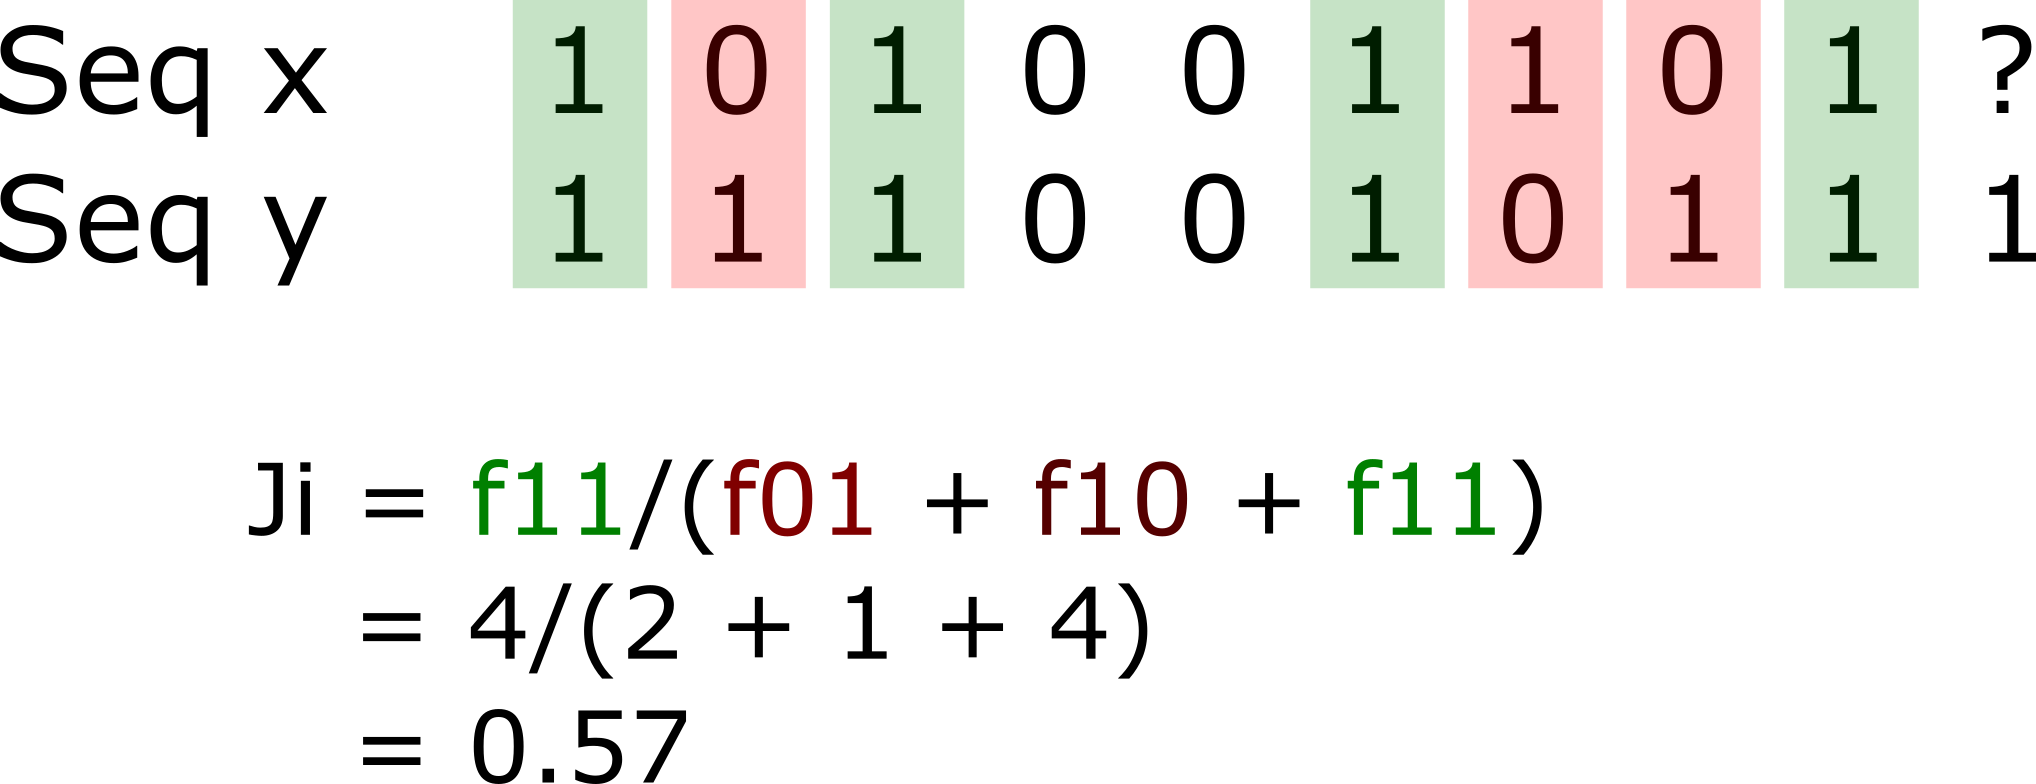
\includegraphics[scale = 1.3]{Images/jaccard}
    \newline
	\caption{An example of Jaccard's similarity index calculation. Note that the shared absence of bands are not taken into account in the calculation of pairwise distances. Jaccard's distance = 1 - J\textsubscript{i}, and therefore 0.43 in this case.}. 
	\label{fig:jaccard}
\end{figure}

% \section{Codon Saturation}

% \label{appendix:saturation}
% \begin{figure}[H]
% 	\centering
% 	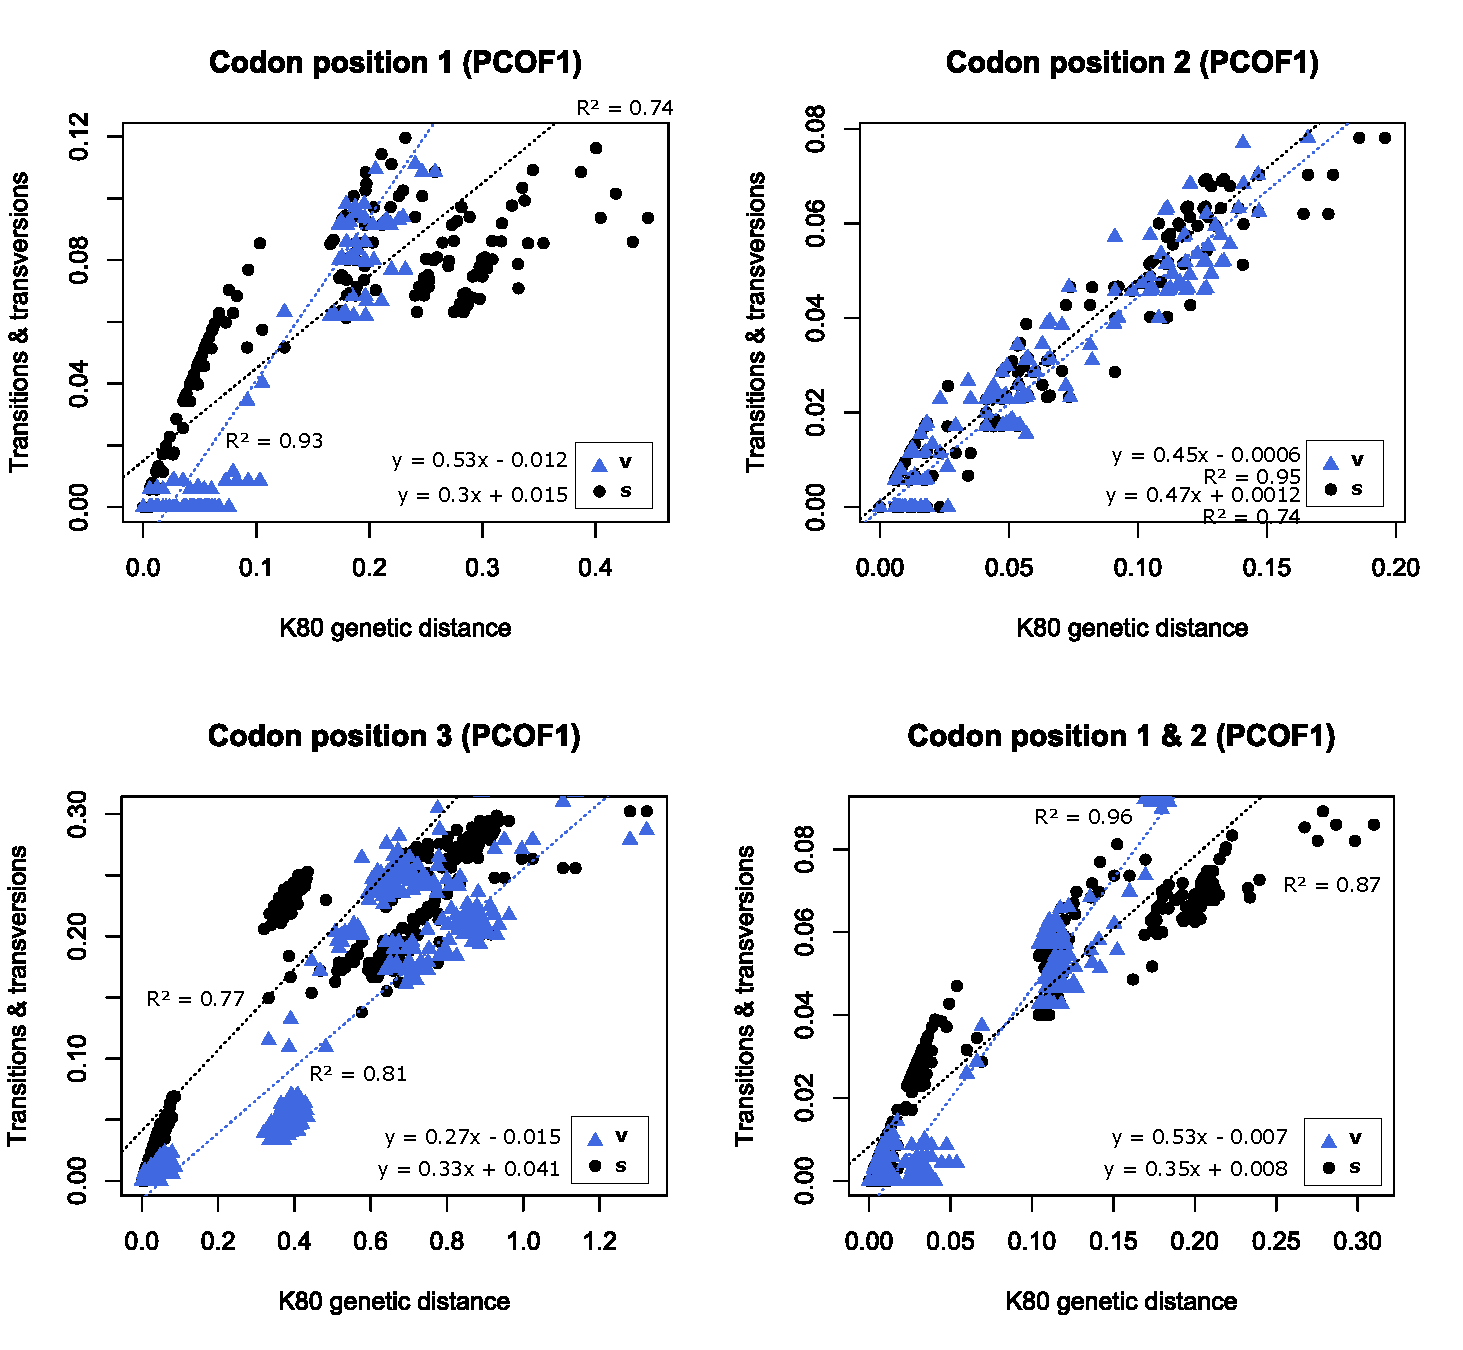
\includegraphics[scale =0.7]{Images/PCOF1_saturation.pdf}
% 	\caption{Transitions (s) and transversions (v) plotted against the K80 genetic distance for the PCOF1 gene at codon positions 1, 2, 3 and 1 \& 2. Equations of the best fit lines are shown, as well as the R\textsuperscript{2} value.}  
% 	\label{fig:pcof1_saturation}
% \end{figure}

% \begin{figure}[H]
% 	\centering
% 	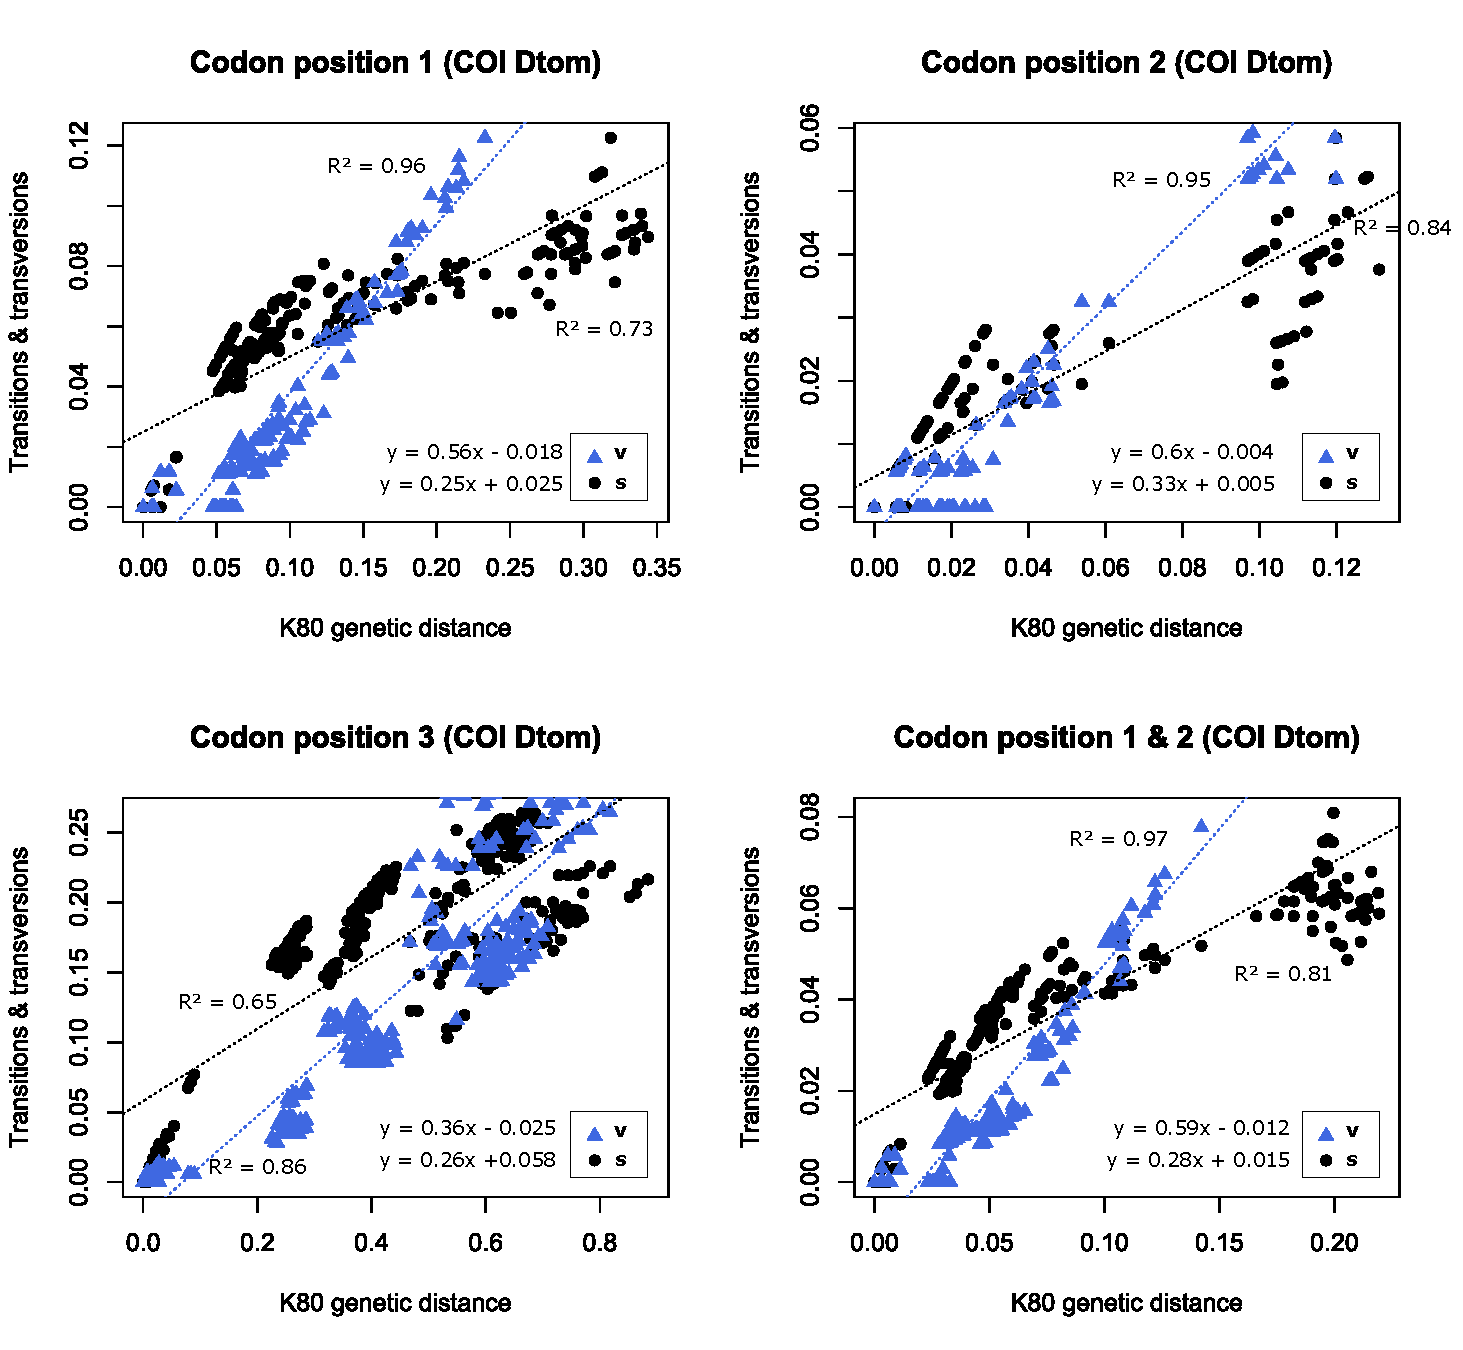
\includegraphics[scale =0.7]{Images/COIDtom_saturation.pdf}
% 	\caption{Transitions (s) and transversions (v) plotted against the K80 genetic distance for the COI (Dtom) gene at codon positions 1, 2, 3 and 1 \& 2. Equations of the best fit lines are shown, as well as the R\textsuperscript{2} value.} 
% 	\label{fig:co1_dtom_saturation}
% \end{figure}

\section{Codon saturation}

\vspace{0.5cm}
\begin{table}[H]
\renewcommand{\arraystretch}{0.4}
\caption{Codon saturation results from DAMBE for the protein-coding COI-A and COI-B gene regions. A significant p-value and an Iss value $<$ the Iss.cSym value means that there is little saturation present.}
\label{tab:saturation}
\centering
\begin{tabular}{@{}lllllll@{}}
\toprule
 & \textbf{NumOTU} & \textbf{Iss} & \textbf{Iss.cSym} & \textbf{T} & \textbf{DF} & \textbf{P} \\ \midrule
\textbf{\begin{tabular}[c]{@{}l@{}}Codon\\ Position 1\end{tabular}} & \textbf{4} & 0.357 & 0.777 & 10.403 & 200 & 0 \\
 & \textbf{8} & 0.327 & 0.734 & 10.155 & 200 & 0 \\
 & \textbf{16} & 0.311 & 0.643 & 8.428 & 200 & 0 \\
\textbf{\begin{tabular}[c]{@{}l@{}}Codon\\ Position 2\end{tabular}} & \textbf{4} & 0.273 & 0.777 & 12.203 & 200 & 0 \\
 & \textbf{8} & 0.227 & 0.734 & 12.727 & 200 & 0 \\
 & \textbf{16} & 0.228 & 0.643 & 10.415 & 200 & 0 \\
\textbf{\begin{tabular}[c]{@{}l@{}}Codon\\ Position 3\end{tabular}} & \textbf{4} & 0.578 & 0.777 & 4.956 & 200 & 0 \\
 & \textbf{8} & 0.539 & 0.734 & 4.979 & 200 & 0 \\
 & \textbf{16} & 0.534 & 0.643 & 2.843 & 200 & 0 \\
\textbf{\begin{tabular}[c]{@{}l@{}}Codon\\ Position 1 \& 2\end{tabular}} & \textbf{4} & 0.334 & 0.788 & 14.989 & 401 & 0 \\
 & \textbf{8} & 0.274 & 0.742 & 16.002 & 401 & 0 \\
 & \textbf{16} & 0.260 & 0.702 & 15.465 & 401 & 0 \\ \bottomrule
\end{tabular}
\end{table}

\begin{landscape}
\begin{figure}[]
	\centering
	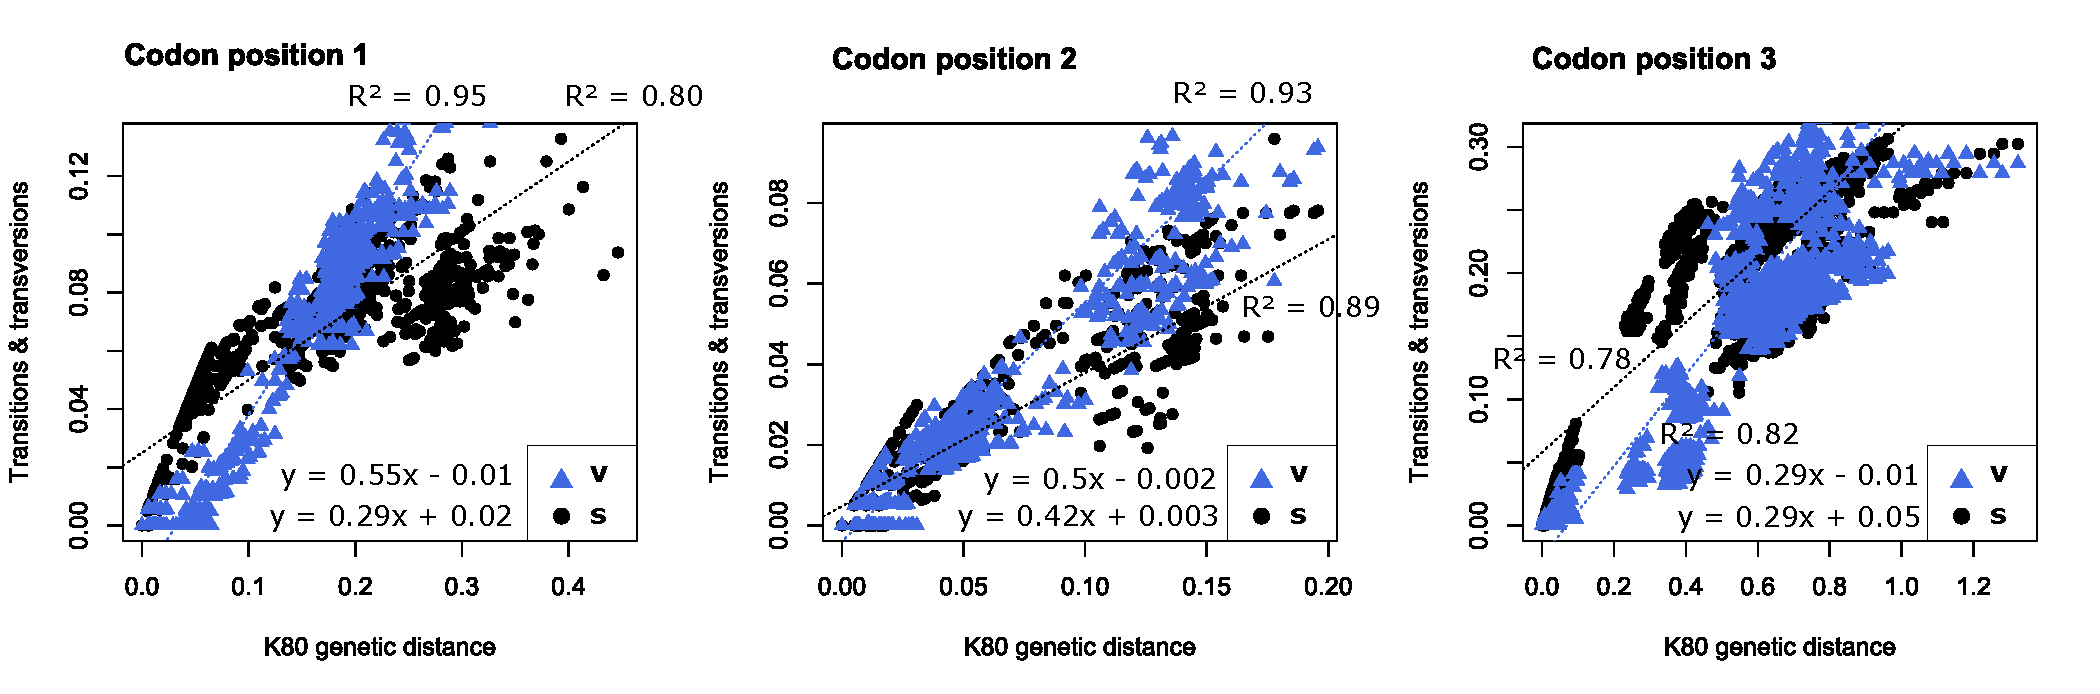
\includegraphics[scale =0.75]{Images/saturation_COI.pdf}
	\caption{Saturation graphs for codon positions 1 to 3 for the COI gene region; showing the relationship between genetic distance and the rate of transitions (s) and transversions (v).}
	\label{fig:COI_saturation_graphs}
\end{figure}
\end{landscape}


% \section{Barcode testing thresholds}

% \begin{figure}[H]
% 	\centering
% 	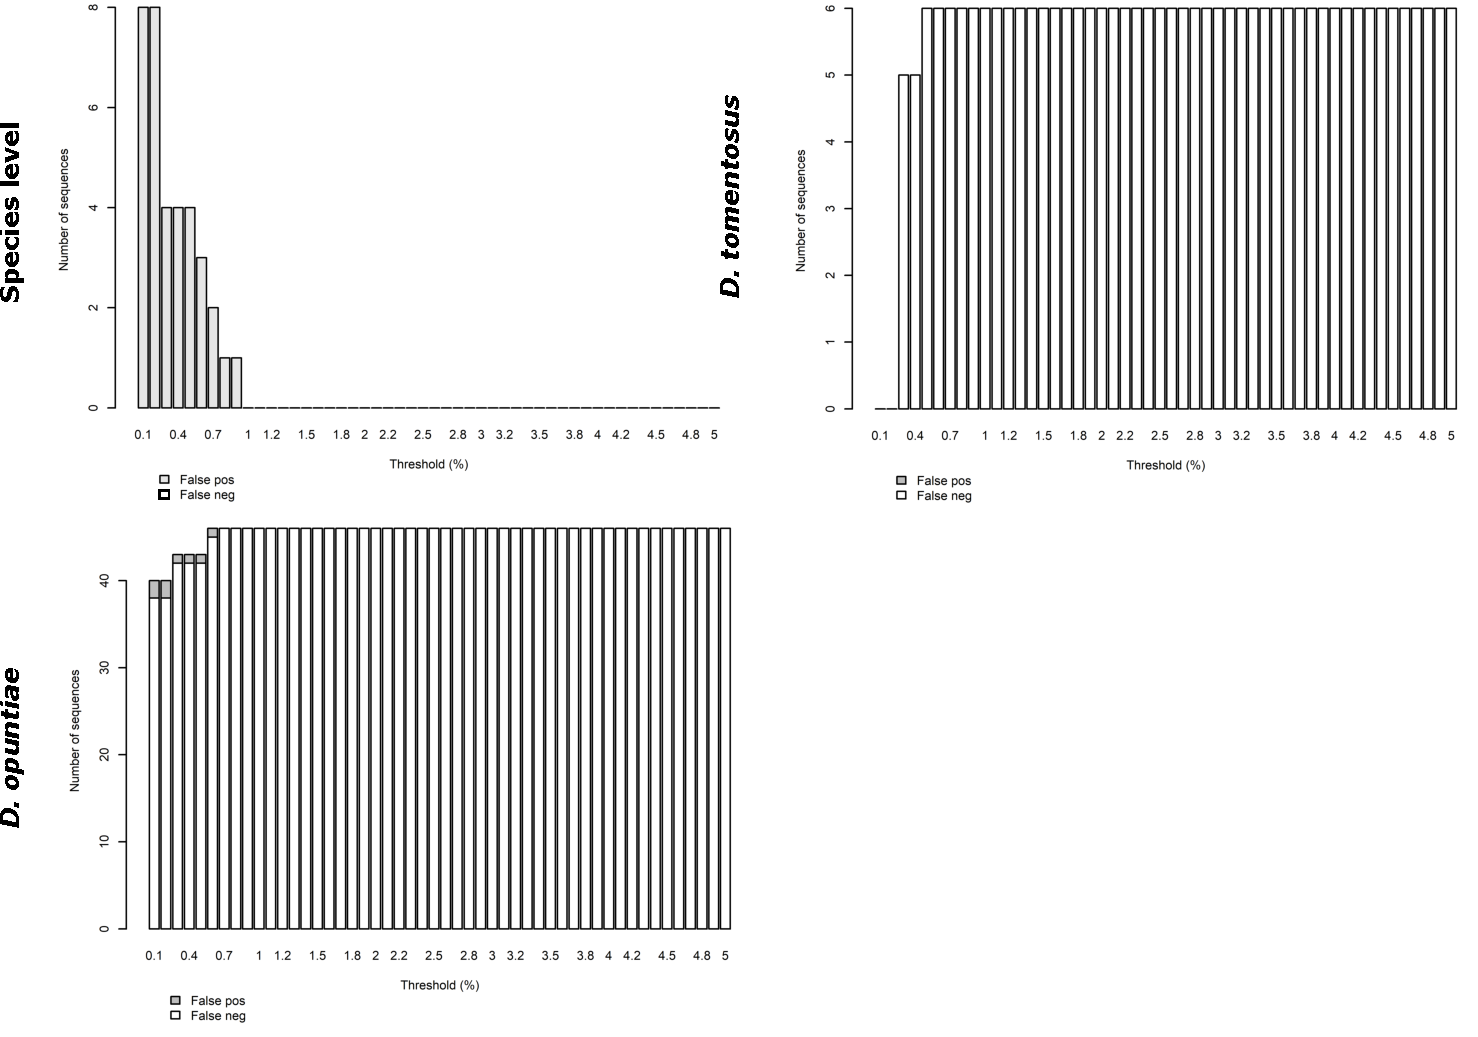
\includegraphics[scale =0.7]{Images/12S_thresholds.pdf}
% 	\caption{Genetic distance threshold values for the 12S gene at the species and lineage level. The optimal threshold percentage at the species level is at 1\% and 0.2\% for \textit{D. tomentosus} lineages. \textit{Dactylopius opuntiae} lineages did not have an optimal threshold value, with a high number of false negatives.} 
% 	\label{fig:12S_thresh}
% \end{figure}

% \begin{figure}[H]
% 	\centering
% 	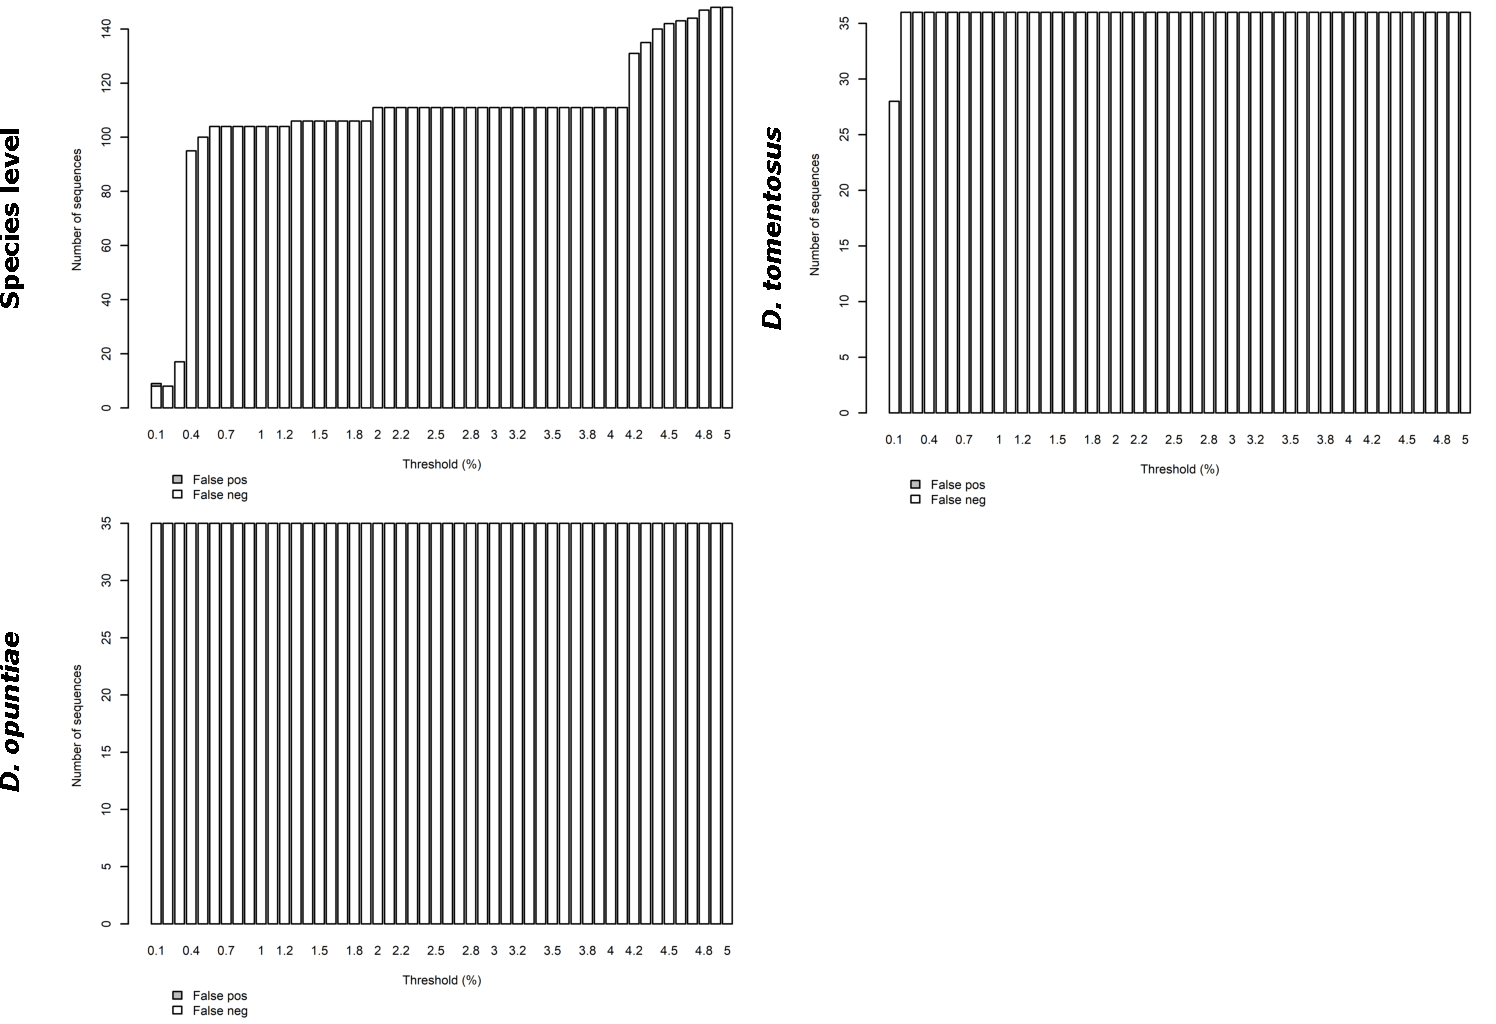
\includegraphics[scale =0.7]{Images/thresholds_18S.pdf}
% 	\caption{Genetic distance threshold values for the 18S gene at the species and lineage level. The optimal threshold value at the species level is 0.2\%. At the lineage level, both \textit{D. tomentosus} and \textit{D. opuntiae} showed a high level of false negatives.} 
% 	\label{fig:18SThresh}
% \end{figure}

% \begin{figure}[H]
% 	\centering
% 	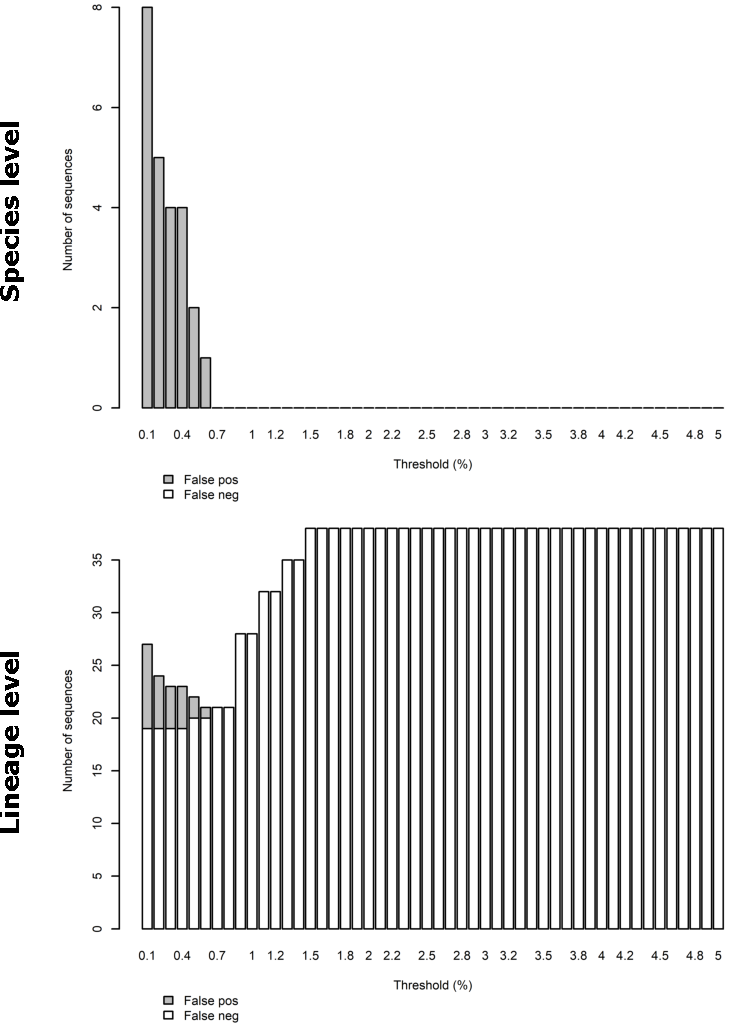
\includegraphics[scale =1]{Images/PCOF1_thresholds.pdf}
% 	\caption{Genetic distance threshold values for the PCOF1 \& LepR1 at the lineage and species level. The optimal threshold value at the species level is 0.7\%. The lineage level (\textit{D. opuntiae}) showed a high number of false negatives.} 
% 	\label{fig:pcof1Thresholds}
% \end{figure}

% \begin{figure}[H]
% 	\centering
% 	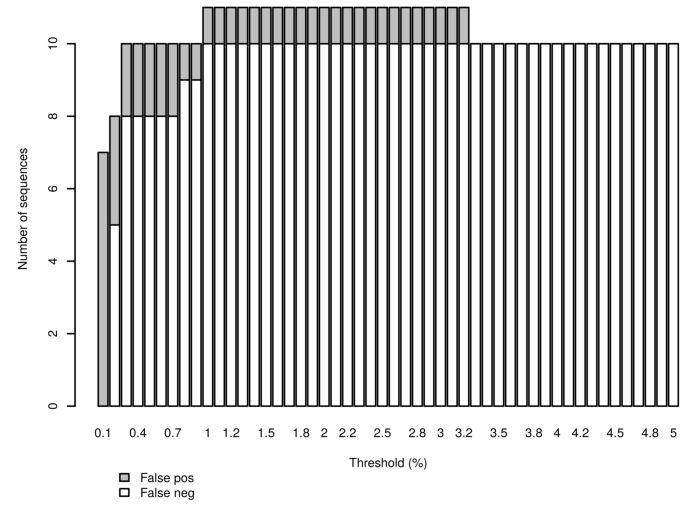
\includegraphics[scale =0.8]{Images/thresholdGraph_DTOM2.pdf}
% 	\caption{Genetic distance threshold values for DTOMf \& HCO2198 at the \textit{D. tomentosus} lineage level. `Bigelovii' and `echinocarpa x acanthocarpa' are treated as separate lineages.} 
% 	\label{fig:COIDTOM_thresh}
% \end{figure}

% \begin{figure}[H]
% 	\centering
% 	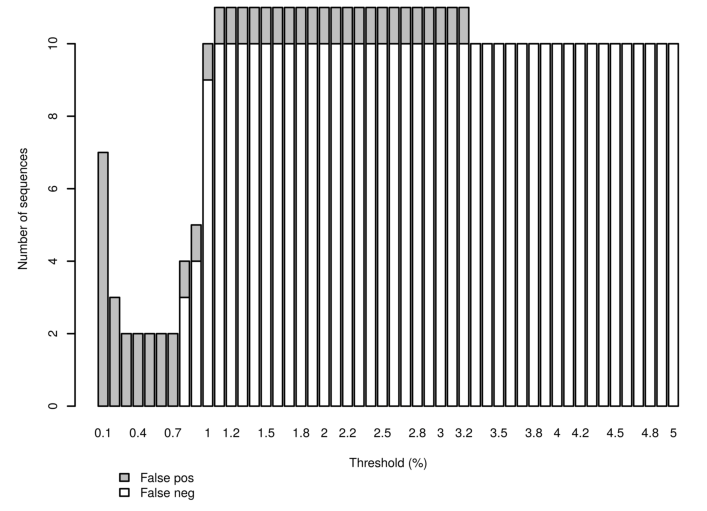
\includegraphics[scale =0.8]{Images/thresholdGraph2.pdf}
% 	\caption{Genetic distance threshold values for DTOMf \& HCO2198 at the \textit{D. tomentosus} lineage level. `Bigelovii' and `echinocarpa x acanthocarpa' are grouped as one lineage.} 
% 	\label{fig:COIDTOM_thresh2}
% \end{figure}

% \begin{figure}[H]
% 	\centering
% 	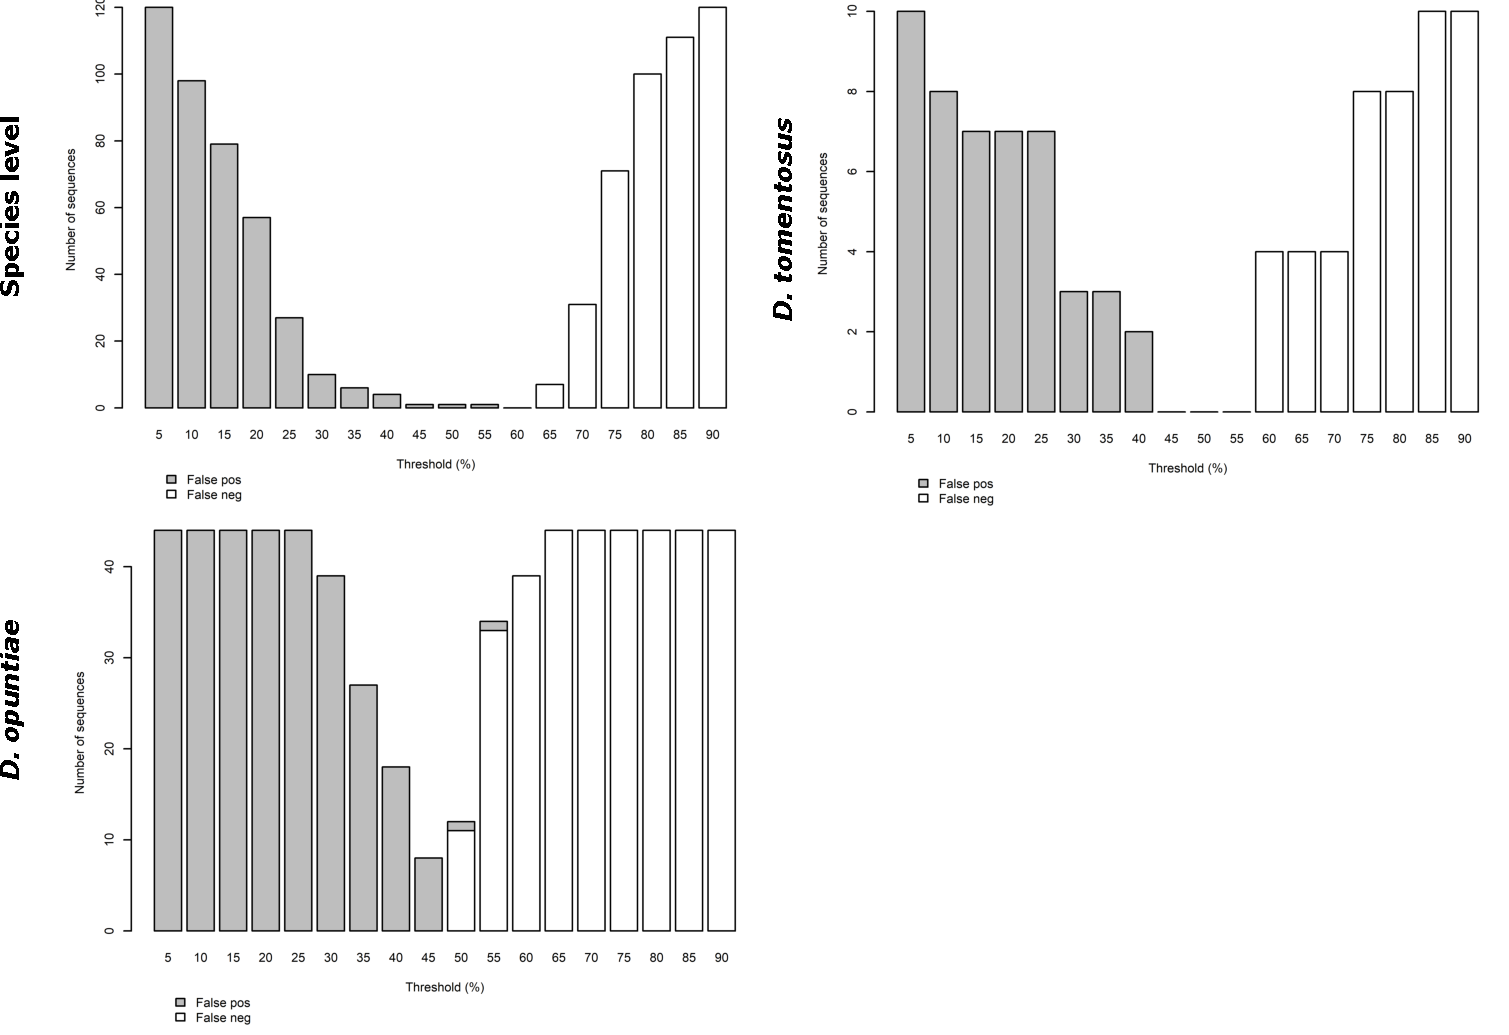
\includegraphics[scale =0.67]{Images/thresholds_issrs.pdf}
% 	\caption{Genetic distance threshold values for the species level, \textit{D. opuntiae} and \textit{D. tomentosus} lineages, for all \textit{Dactylopius} samples.} 
% 	\label{fig:ISSR_thresh}
% \end{figure}

% \section{Barcode Gaps}

% \begin{figure}[H]
% 	\centering
% 	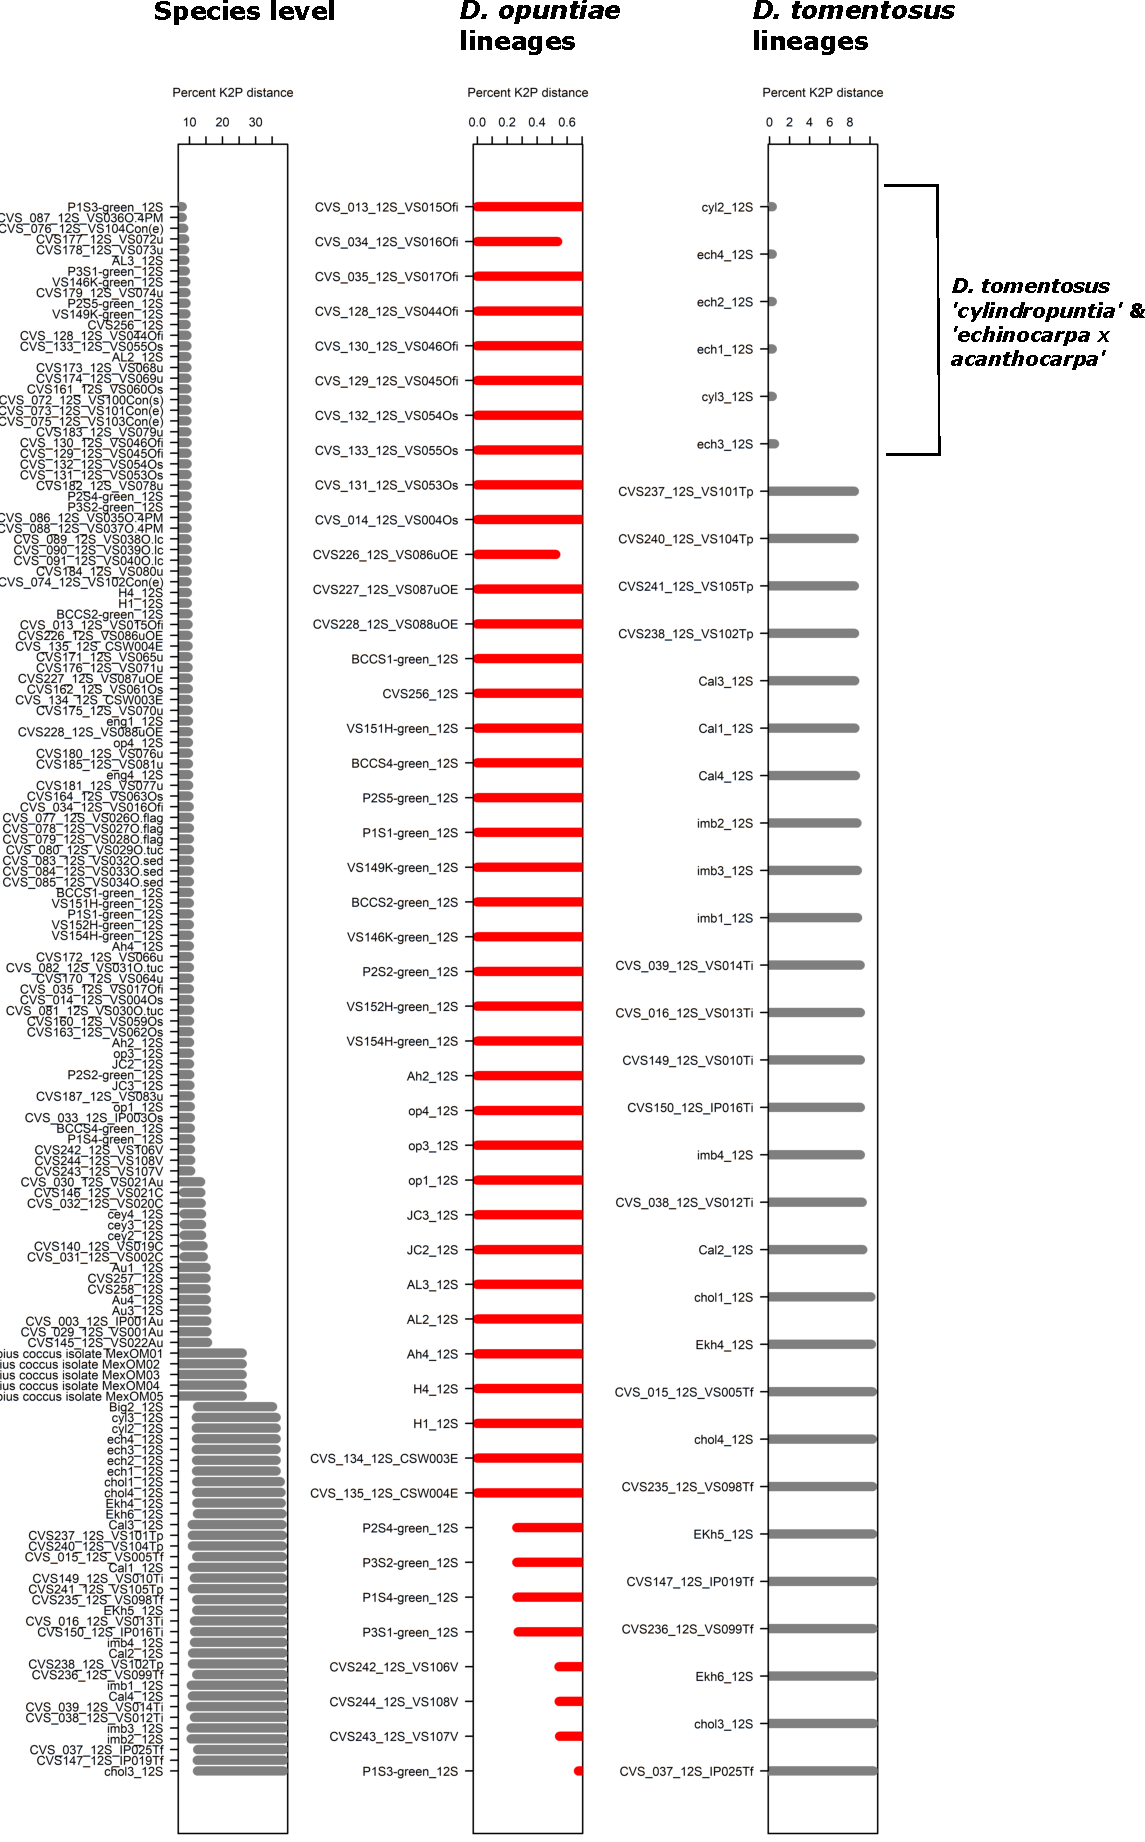
\includegraphics[scale =0.65]{Images/12S_barcode_gaps.pdf}
% 	\caption{Barcode gaps for the 12S gene at the lineage  and species levels. Red bars indicate instances where the intraspecific distance $>$ than the interspecific distance for a particular sequence (i.e. a negative barcode gap). The presence of positive barcode gaps underlies the success of genetic barcoding.} 
% 	\label{fig:12SBarcodeGap}
% \end{figure}

% \begin{figure}[H]
% 	\centering
% 	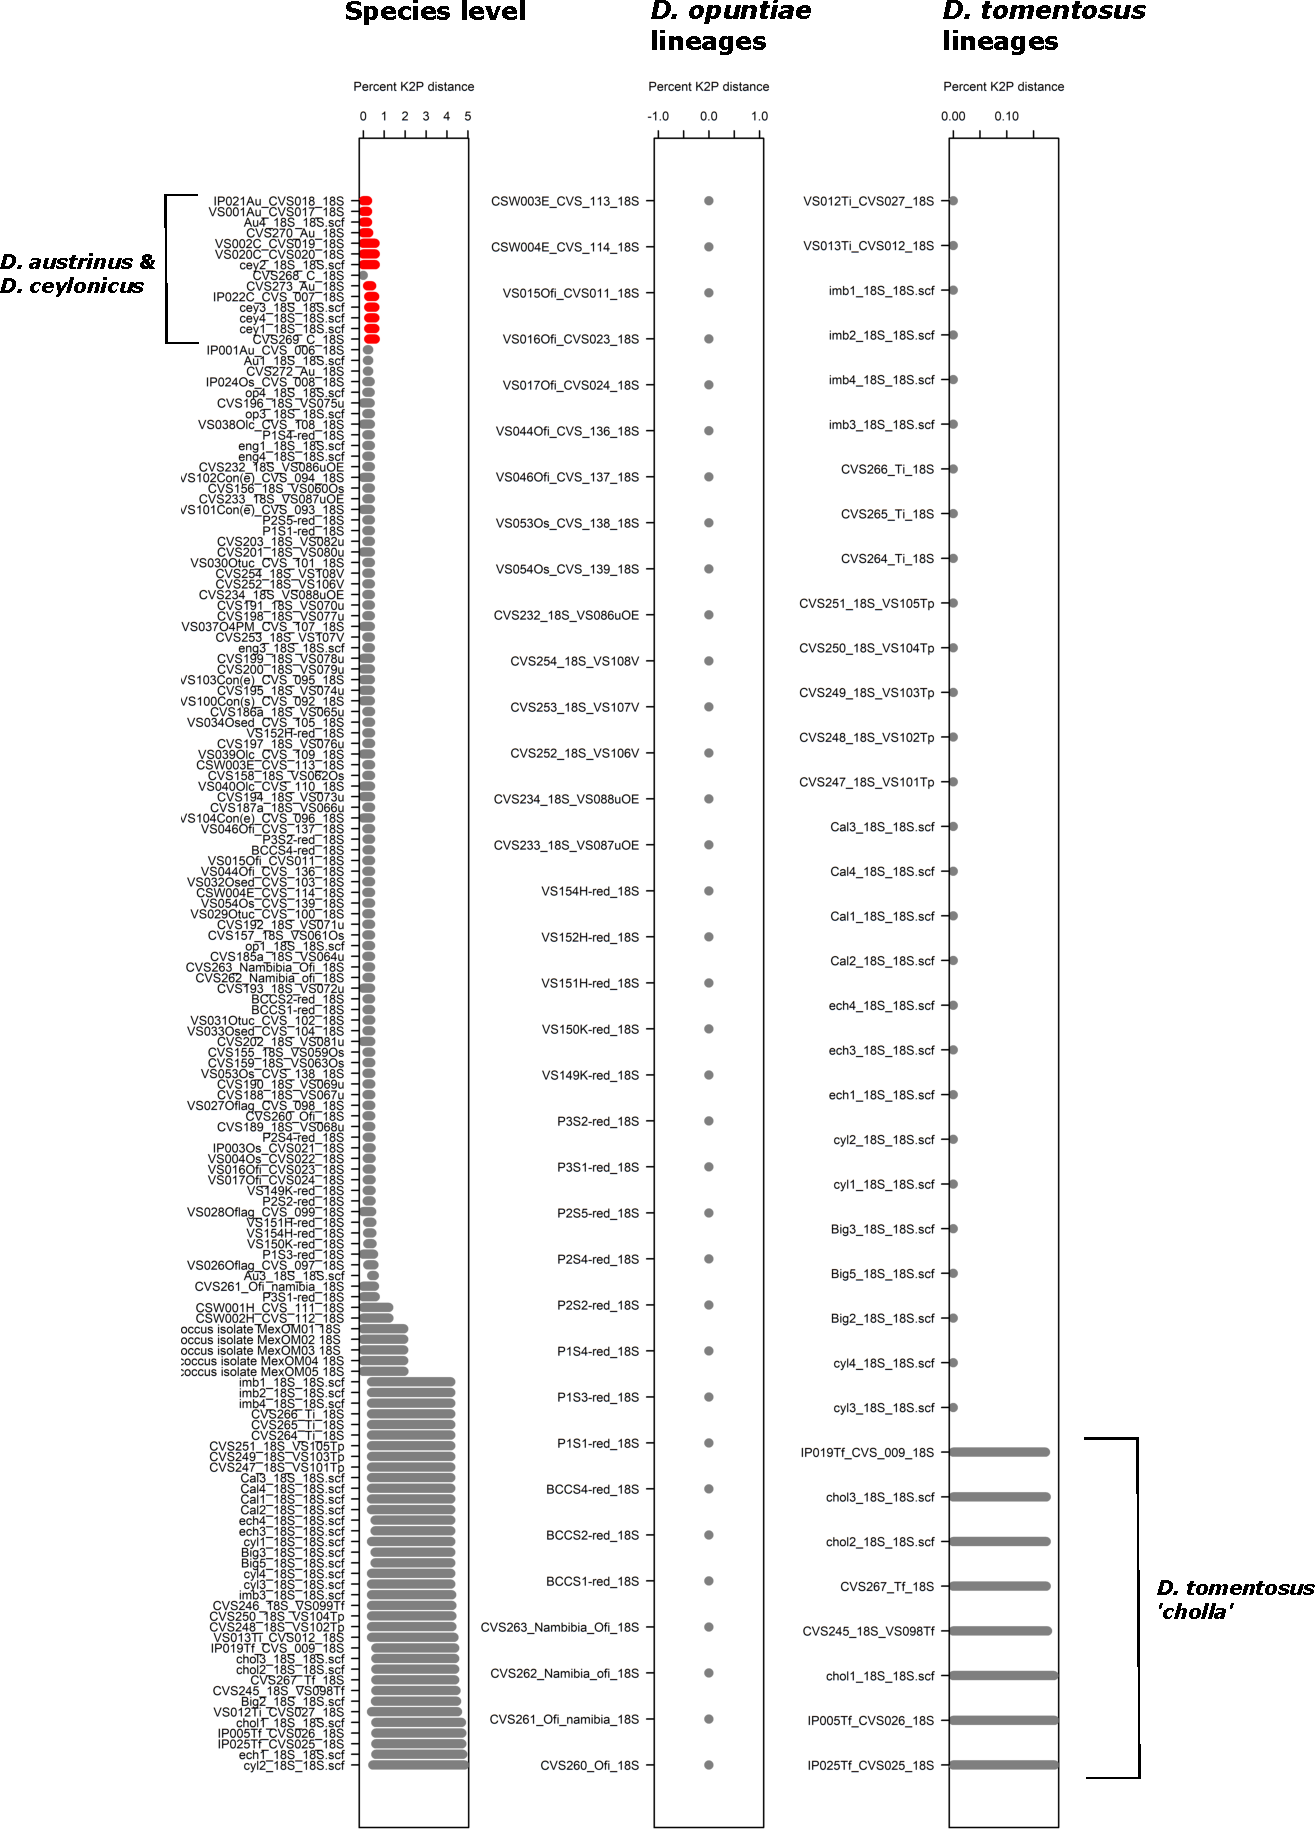
\includegraphics[scale =0.7]{Images/barcode_gaps_18S.pdf}
% 	\caption{Barcode gaps for the 18S gene at the lineage and species level. Note the smaller scale on the lineage-level graphs.} 
% 	\label{fig:18SBarcodeGap}
% \end{figure}

% \begin{figure}[H]
% 	\centering
% 	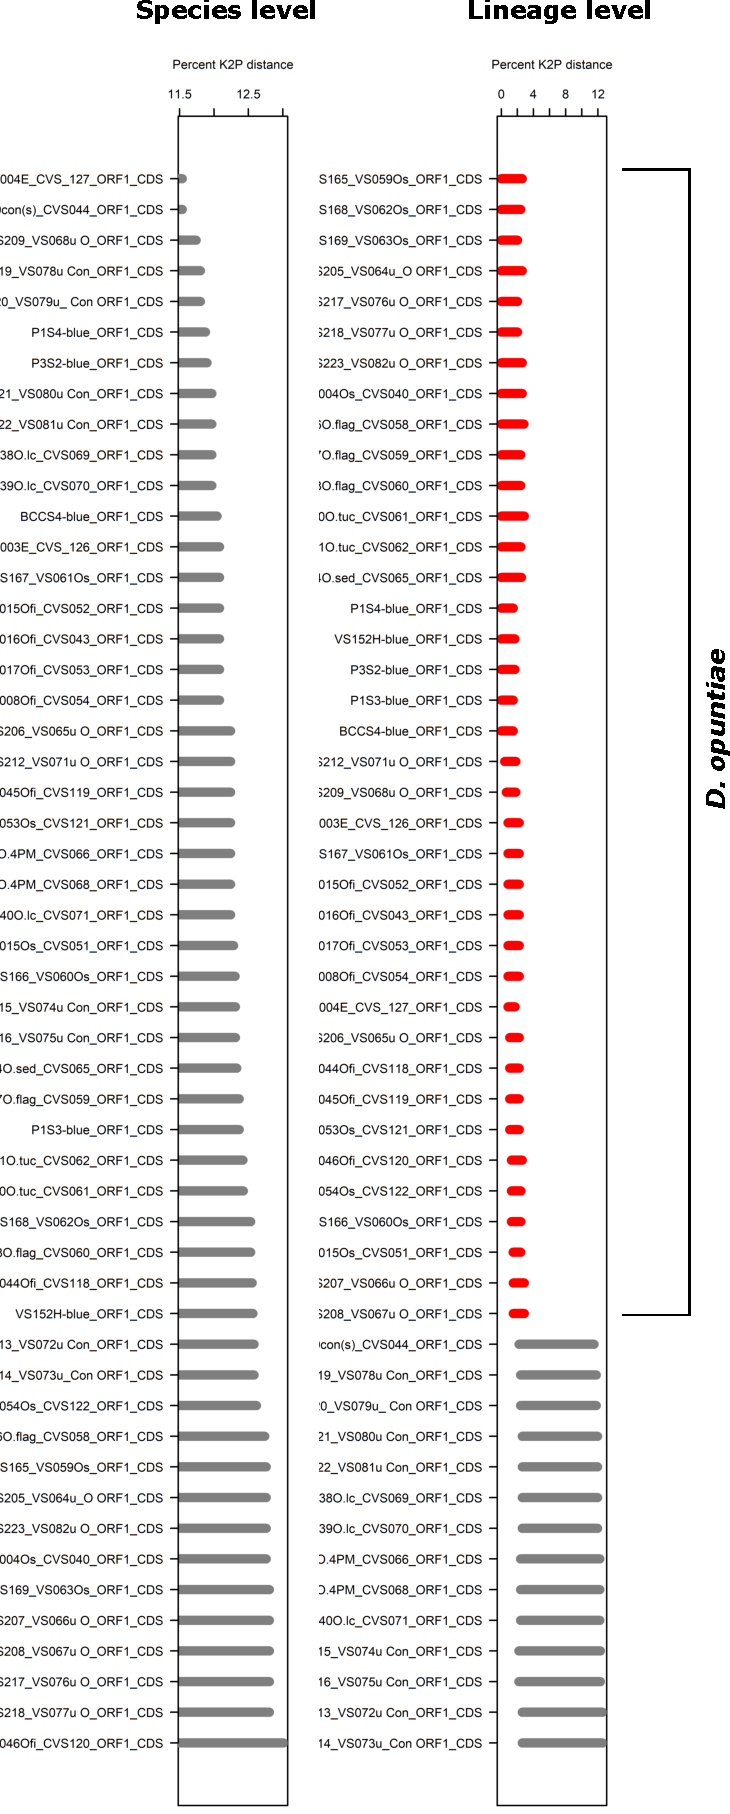
\includegraphics[scale =0.75]{Images/PCOF1_barcode_gaps.pdf}
% 	\caption{Barcode gaps for PCOF1 \& LepR1 at the species and lineage level.} 
% 	\label{fig:COI_barcodeGap}
% \end{figure}

% \newpage

% \begin{figure}[H]
% 	\centering
% 	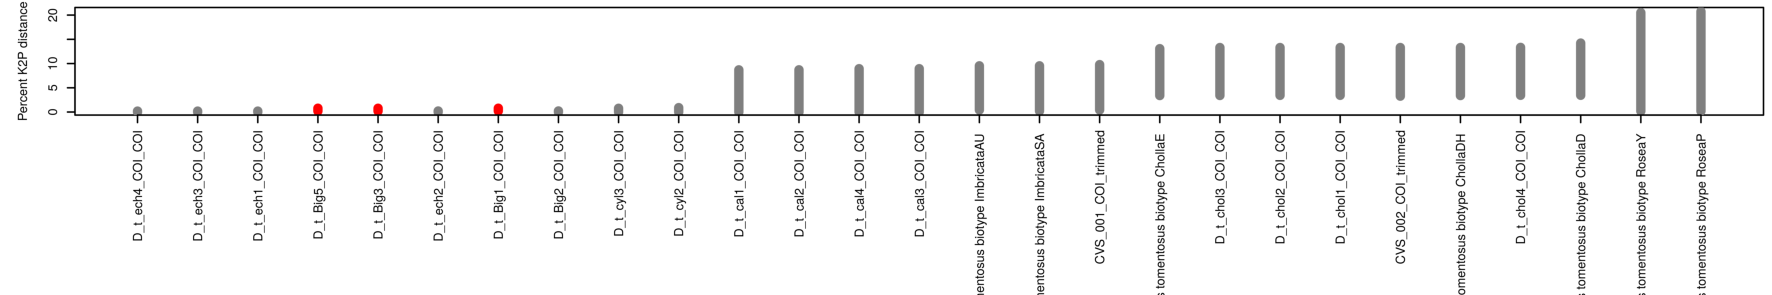
\includegraphics[scale =0.58]{Images/barcodeGap_COIDTOM2.pdf}
% 	\caption{Barcode gaps for DTOMf \& HCO2198 at the lineage (\textit{D. tomentosus}) level.} 
% 	\label{fig:COIDTOM_barcodeGap}
% \end{figure}

\section{ISSR results}

\subsection{Electropherograms}

% \begin{figure}[H]
% 	\centering
% 	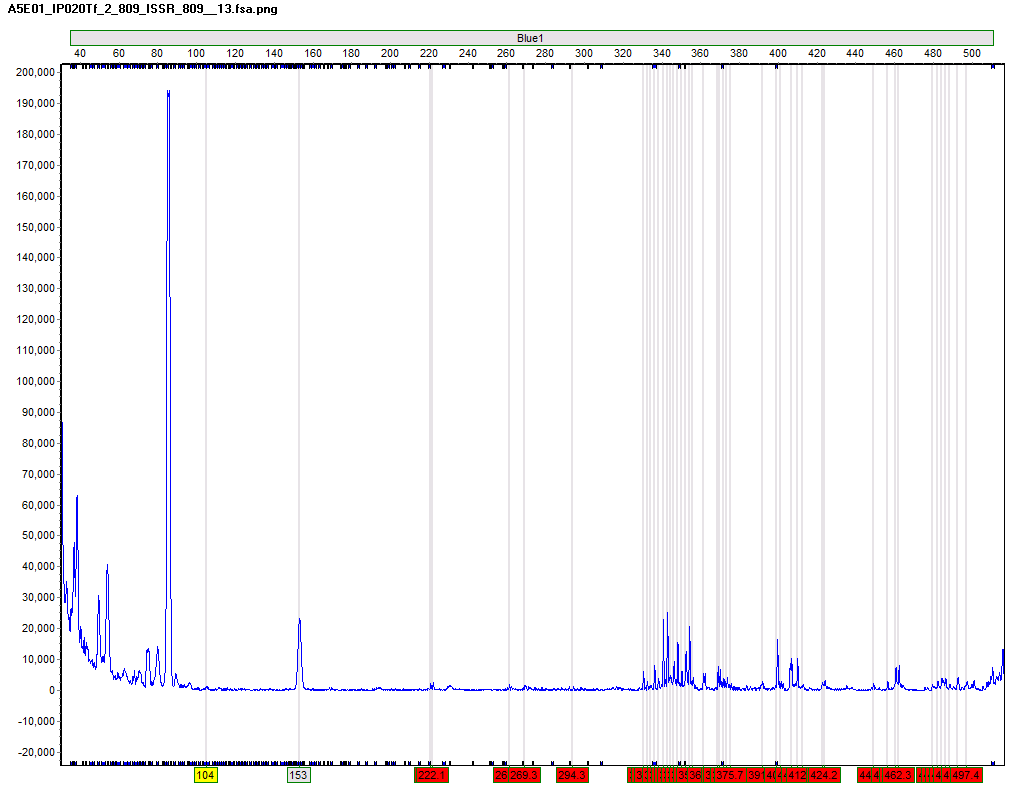
\includegraphics[scale = 0.41]{Images/Tf_electro.png}
%     \newline
% 	\caption{Processed electropherogram for a \textit{Dactylopius tomentosus} `cholla' ISSR sample labelled with 6-FAM\textsuperscript{TM} fluorescent dye. The y-axis represents Relative Fluorescence Units (RFU), and the x-axis displays fragment size in base pairs. Vertical grey lines are peak calls made by GeneMarker\textsuperscript{\textregistered} based on the selected analysis settings.} 
% 	\label{fig:Tf_electro}
% \end{figure}

\begin{figure}[H]
	\centering
	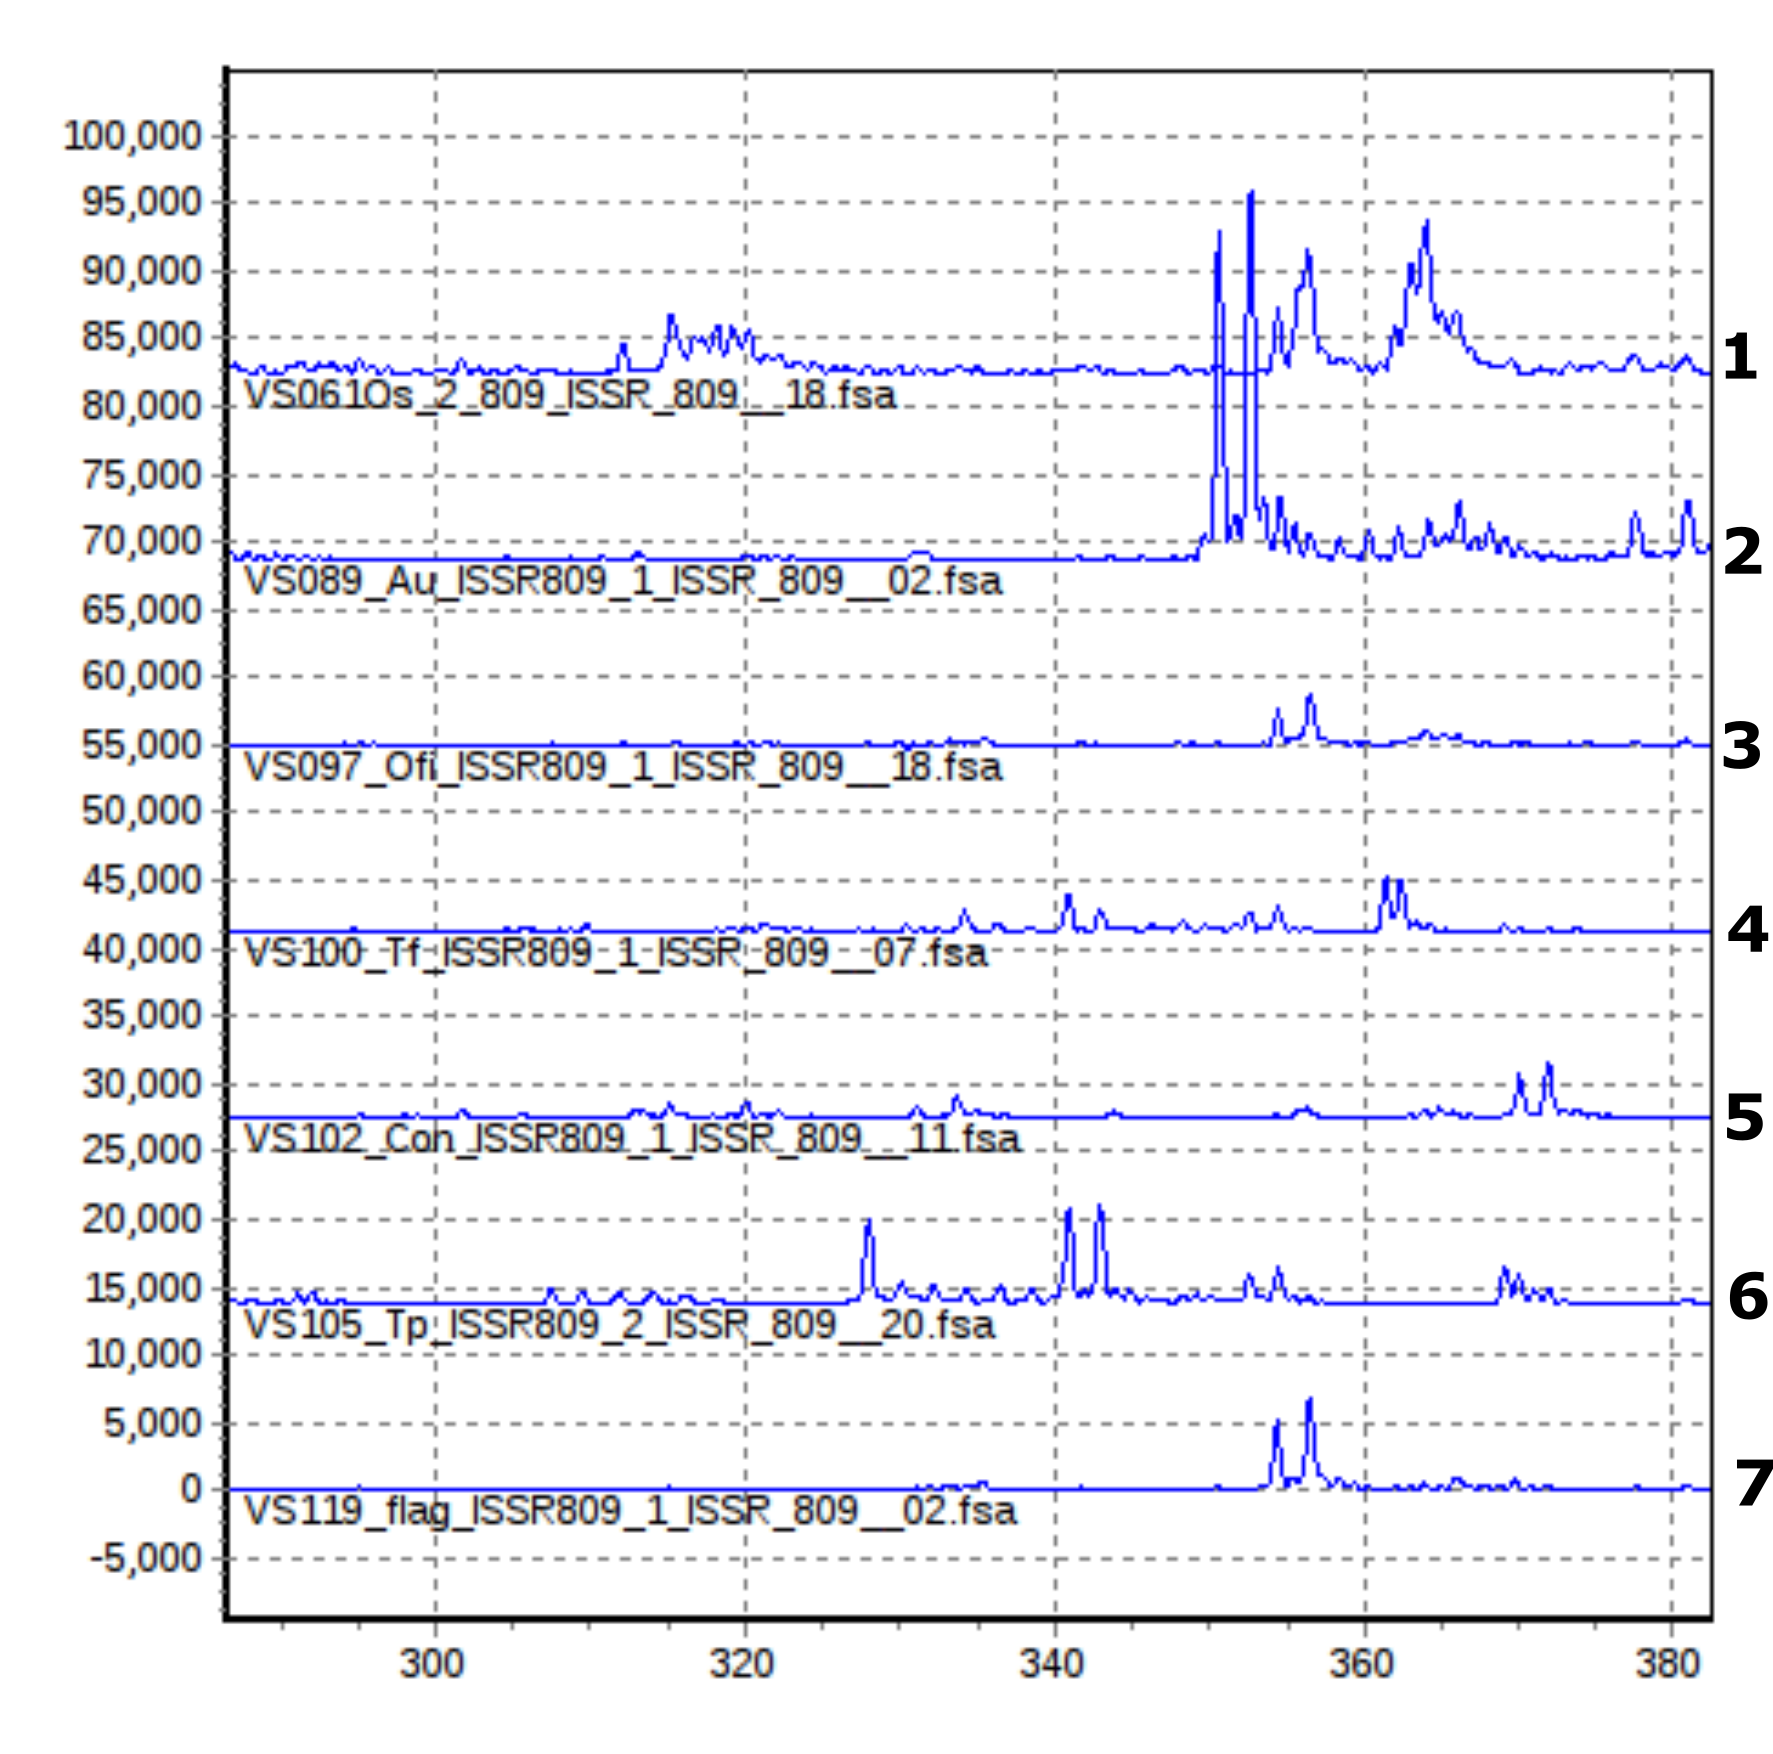
\includegraphics[scale = 1]{Images/overlay_electrophero.png}
	\caption{An overlay view of fragment sizes between 300 and 380 bp for samples (1) \textit{Dactylopius opuntiae} `stricta', (2) \textit{D. austrinus}, (3) \textit{D. opuntiae} `ficus-indica', (4) \textit{D. tomentosus} `cholla', (5) \textit{D. confusus}, (6) \textit{D. tomentosus} `pallida' and (7) \textit{D. opuntiae} collected from Flagstaff (AZ, USA). The y-axis represents Relative Fluorescence Units (RFU), and the x-axis displays fragment size in base pairs.} 
	\label{fig:overlay_electro}
\end{figure}

\subsection{Error rates}
\begin{figure}[H]
	\centering
	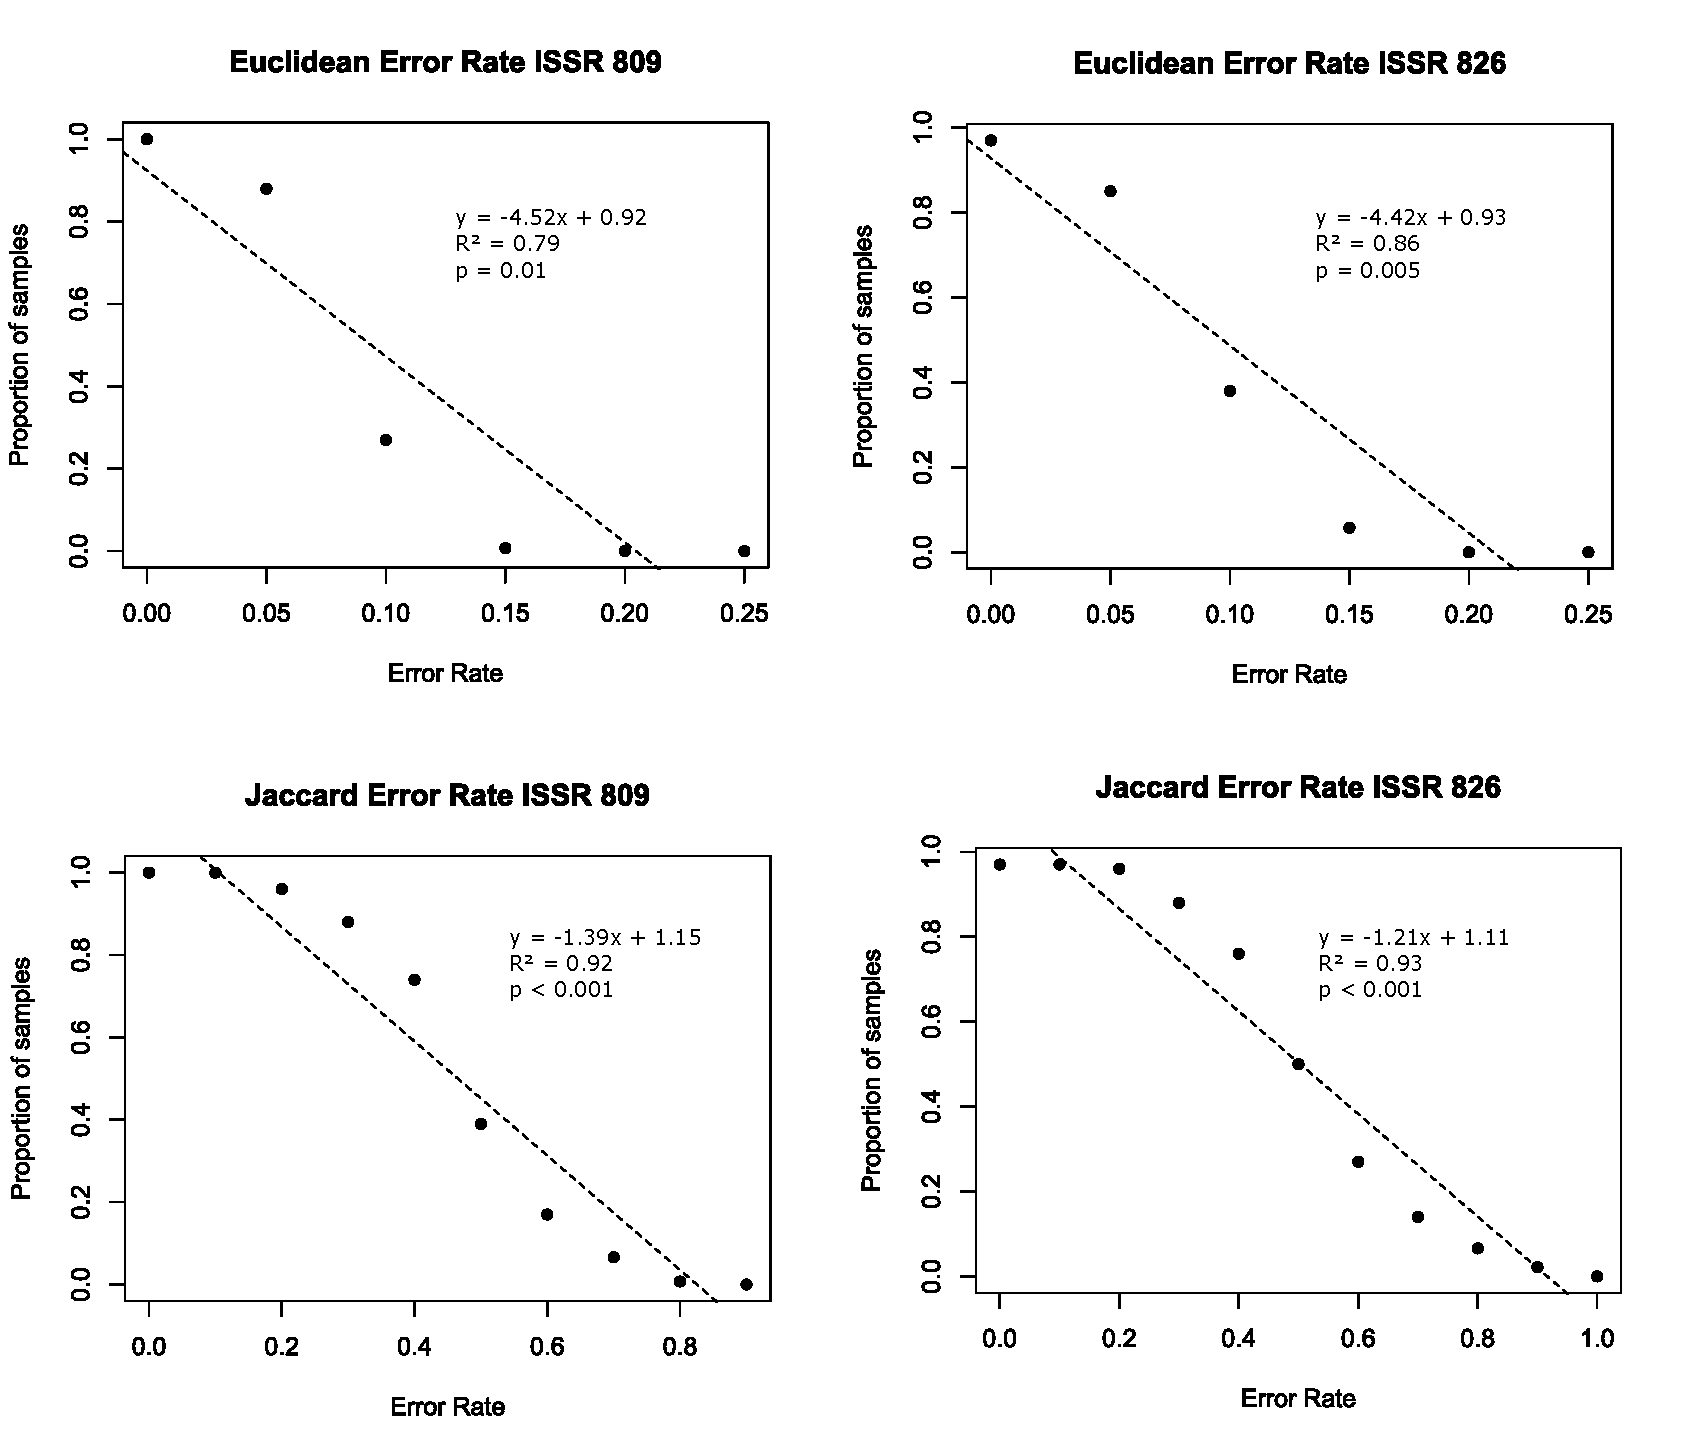
\includegraphics[scale =0.6]{Images/error_rates_graphs.pdf}
	\caption{Euclidean and Jaccard error rates for ISSR primers 826 and 809, showing the proportion of samples greater than a particular error rate. Values are representative of the full data set.}
	\label{fig:error_graphs}
\end{figure}

\begin{figure}[H]
	\centering
	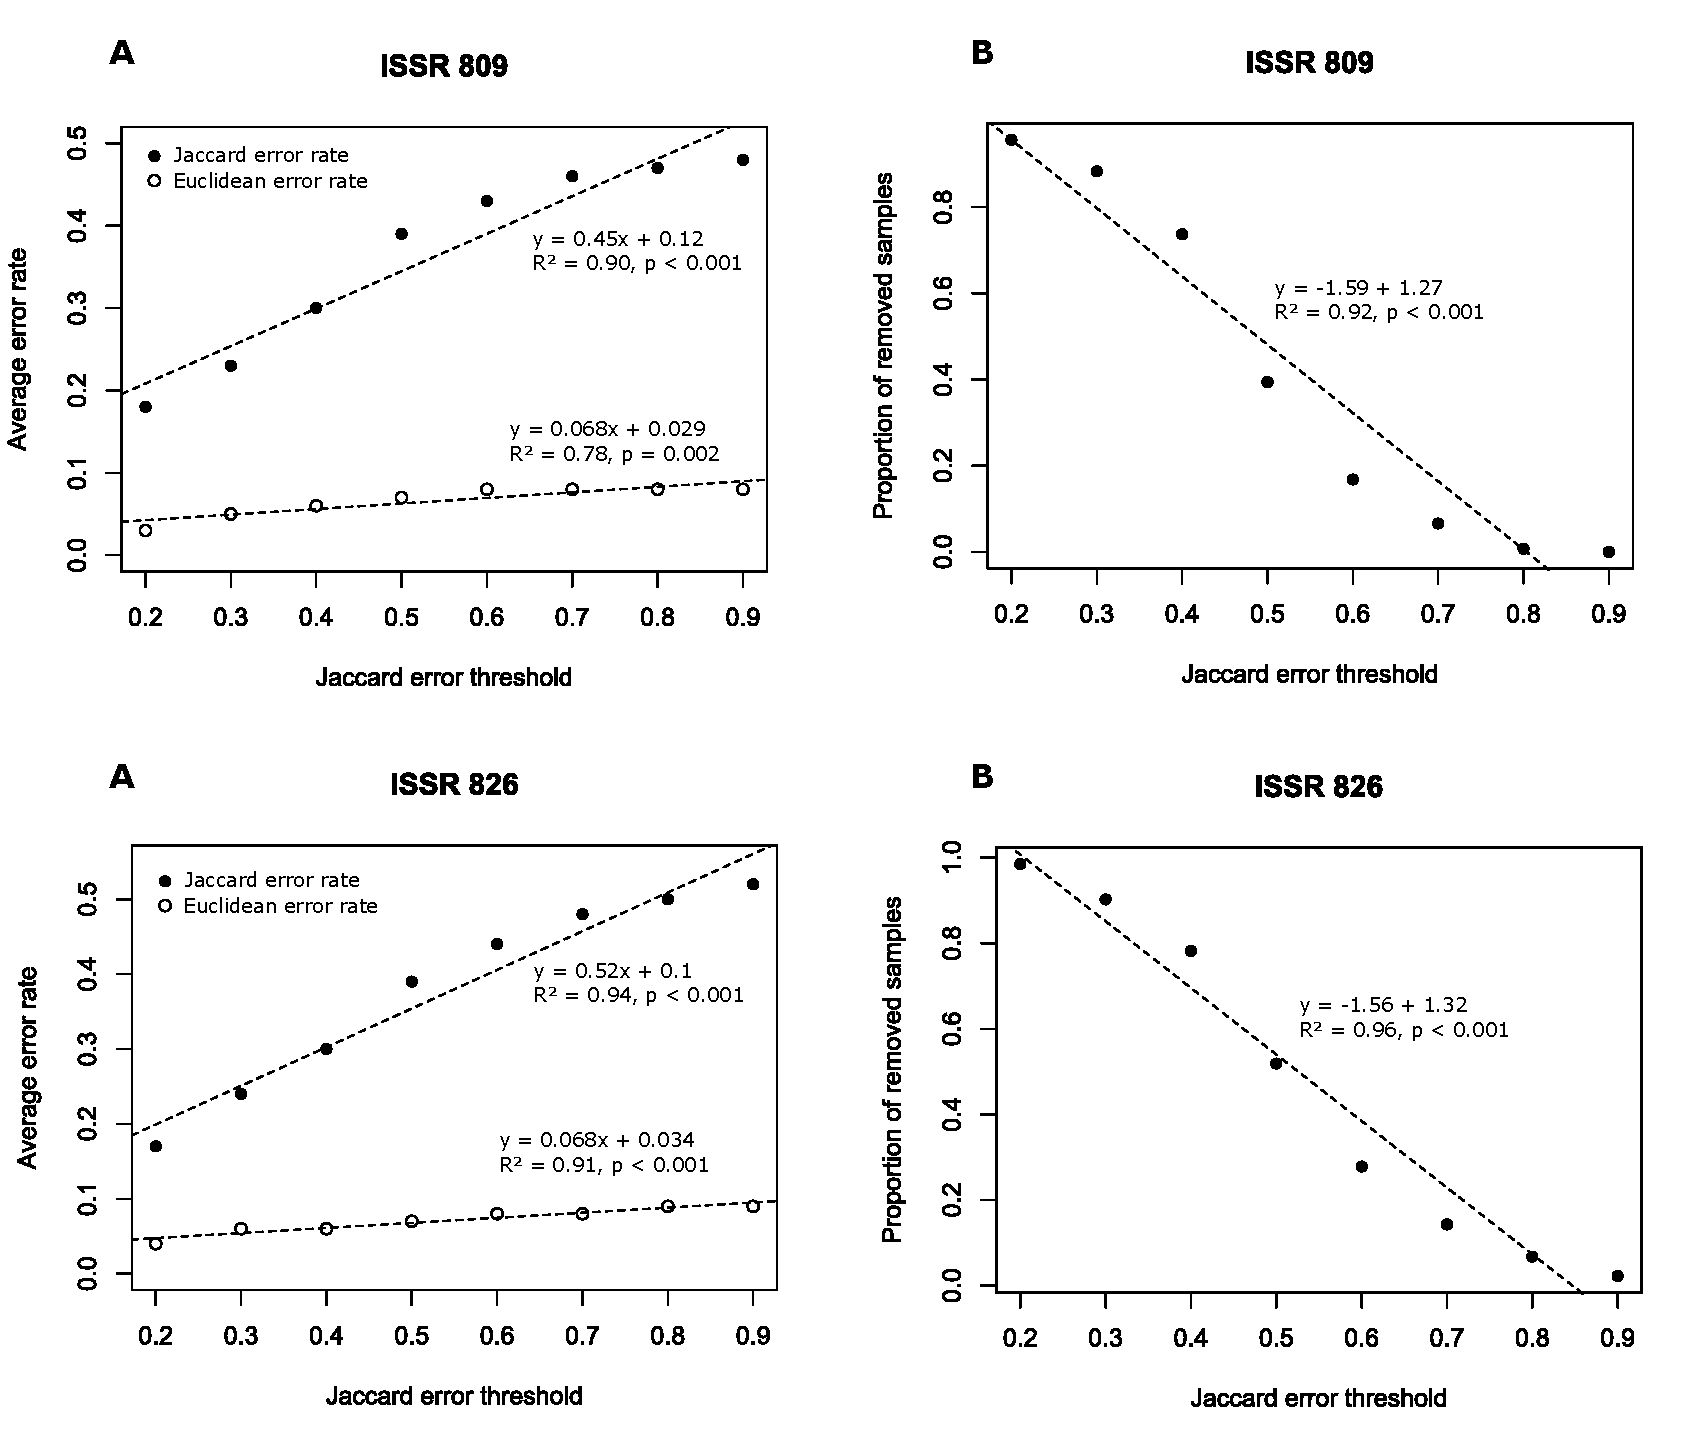
\includegraphics[scale =0.6]{Images/error_stats_graphs.pdf}
	\caption{Graphical representations of the effect of the removal of samples (ISSR 809 and ISSR 826) with a Jaccard error rate greater than a specific threshold on A) the average Jaccard and Euclidean error rates and B) the proportion of removed samples from the data set.}
	\label{fig:error_graphs2}
\end{figure}



\begin{landscape}
\subsection{Splitstree}
\label{appendix:issrSplitstrees}

\begin{figure}[H]
	\centering
	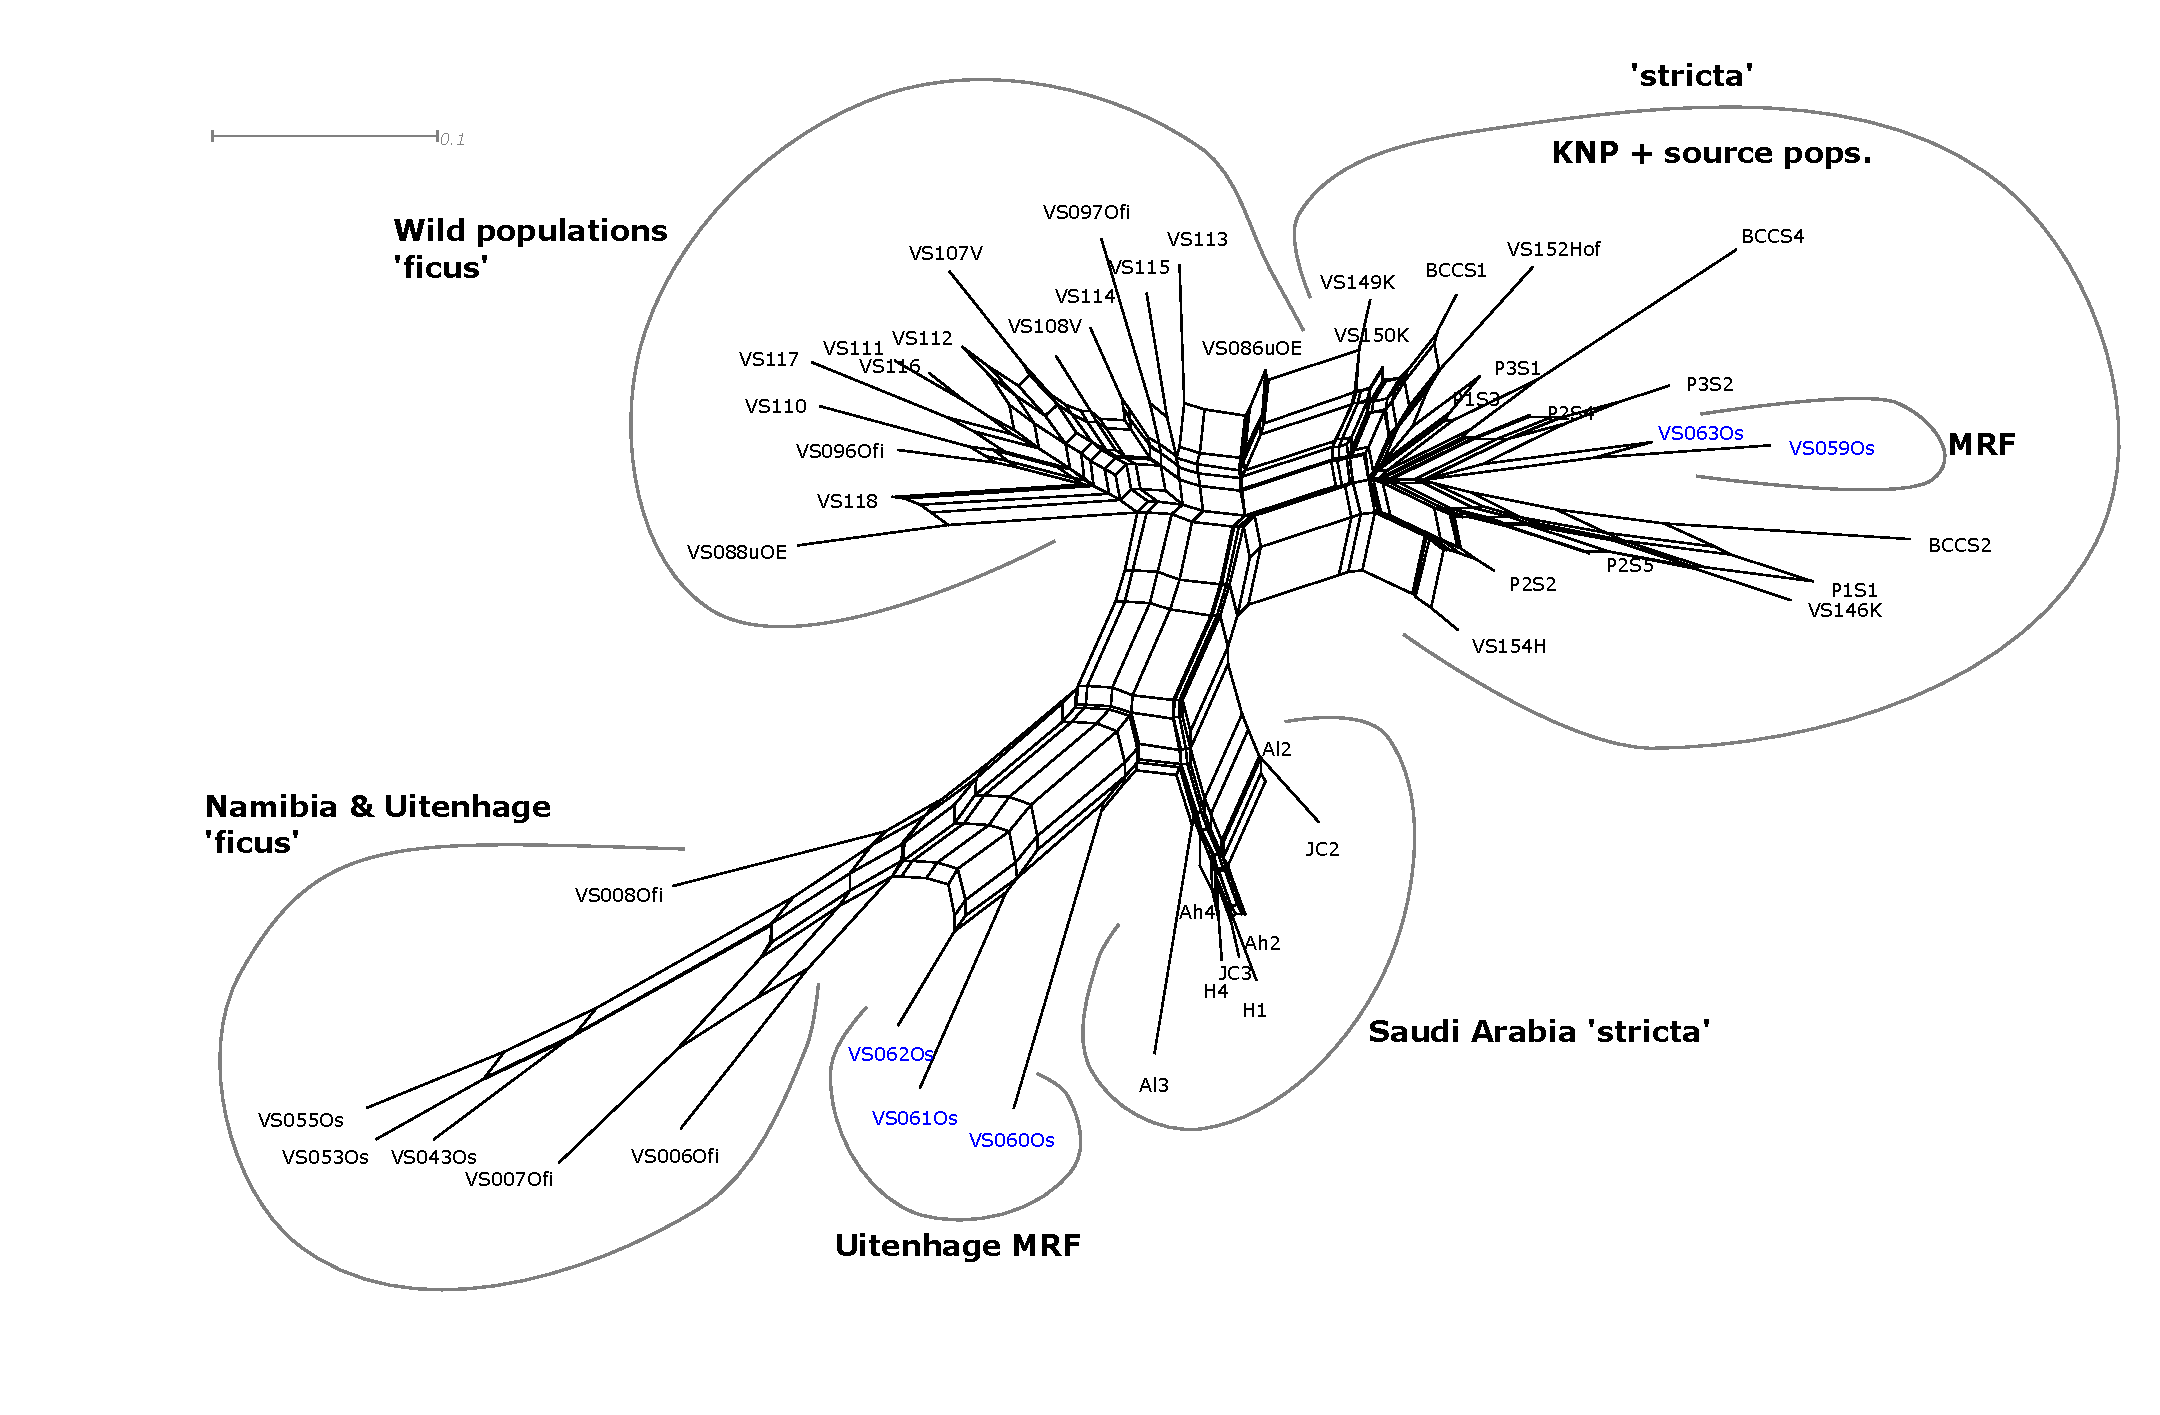
\includegraphics[scale =0.6]{Images/issr809_splitstree.pdf}
	\caption{Splitstree diagram representative of ISSR 809 only. Mass Rearing Facility (MRF) samples are shown in blue. KNP = Kruger National Park, and source pops. = the `stricta' culture kept by Hildegard Klein and John Hoffmann.} 
	\label{fig:issr809_splitstree}
\end{figure}
\end{landscape}


\begin{figure}[H]
	\centering
	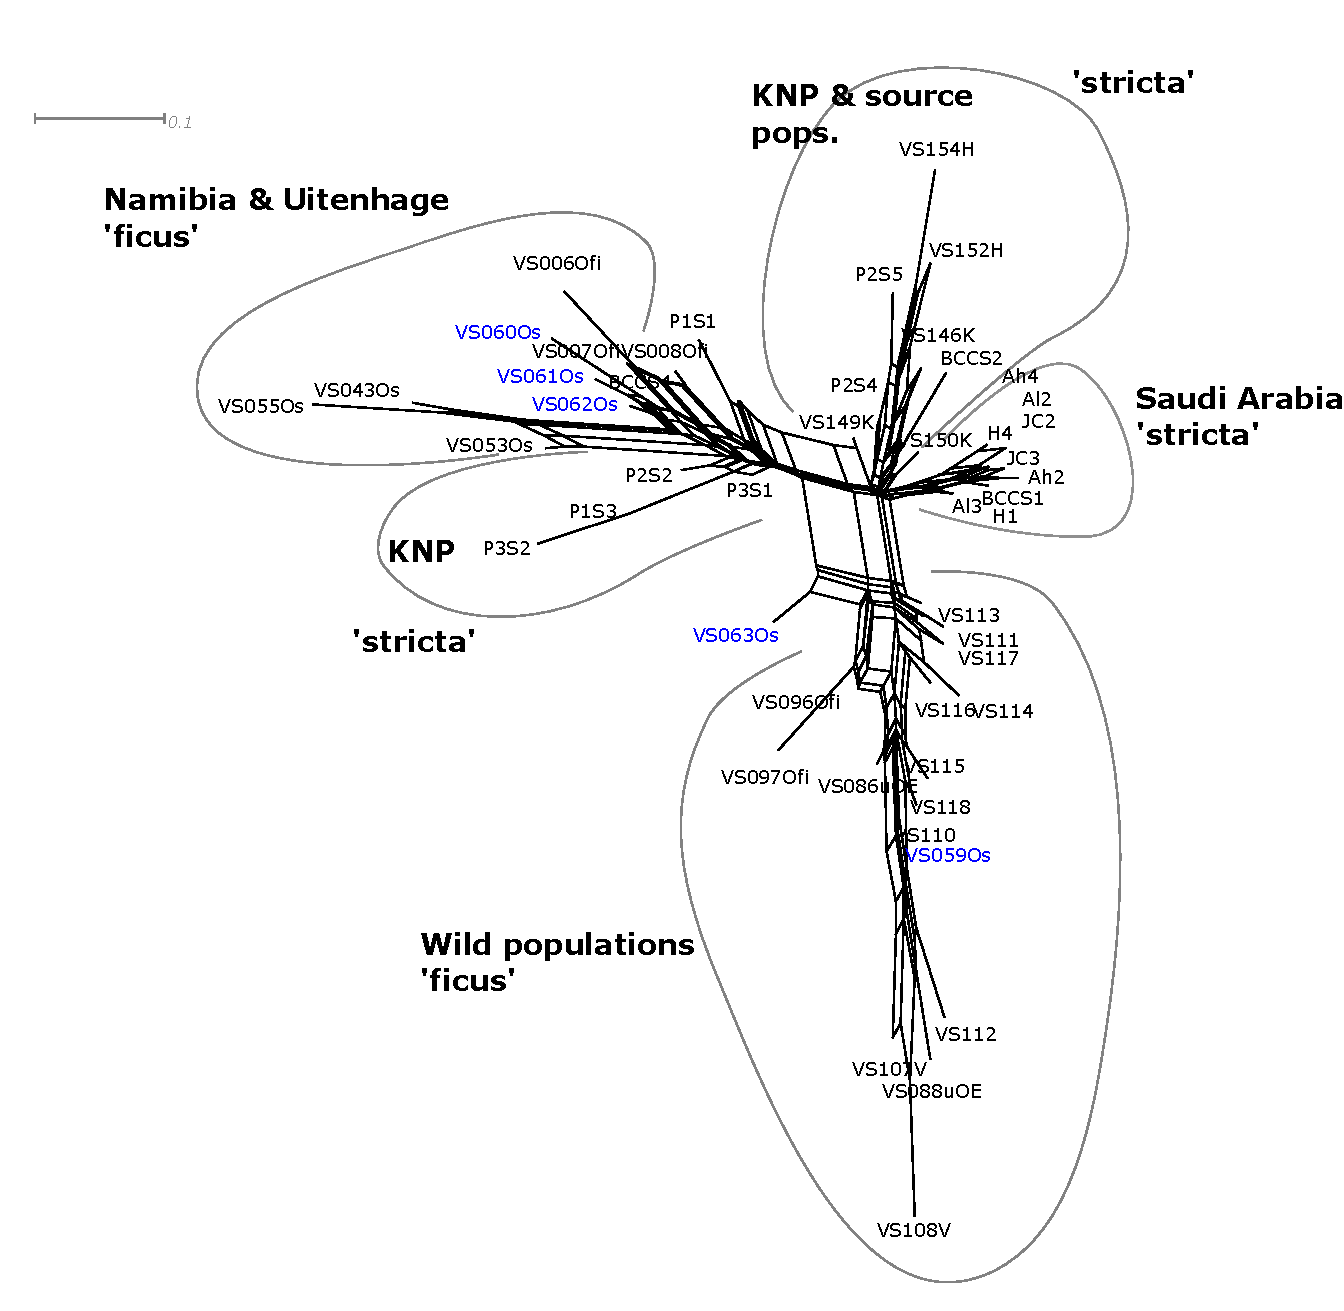
\includegraphics[scale =0.6]{Images/issr826_splitstree.pdf}
	\caption{Splitstree diagram representative of ISSR 826 only. Mass Rearing Facility (MRF) samples are shown in blue. KNP = Kruger National Park, and source pops. = the `stricta' culture kept by Hildegard Klein and John Hoffmann.} 
	\label{fig:issr826_splitstree}
\end{figure}

\begin{landscape}
\subsection{Shepard and scree plots}
\begin{figure}[H]
	\centering
	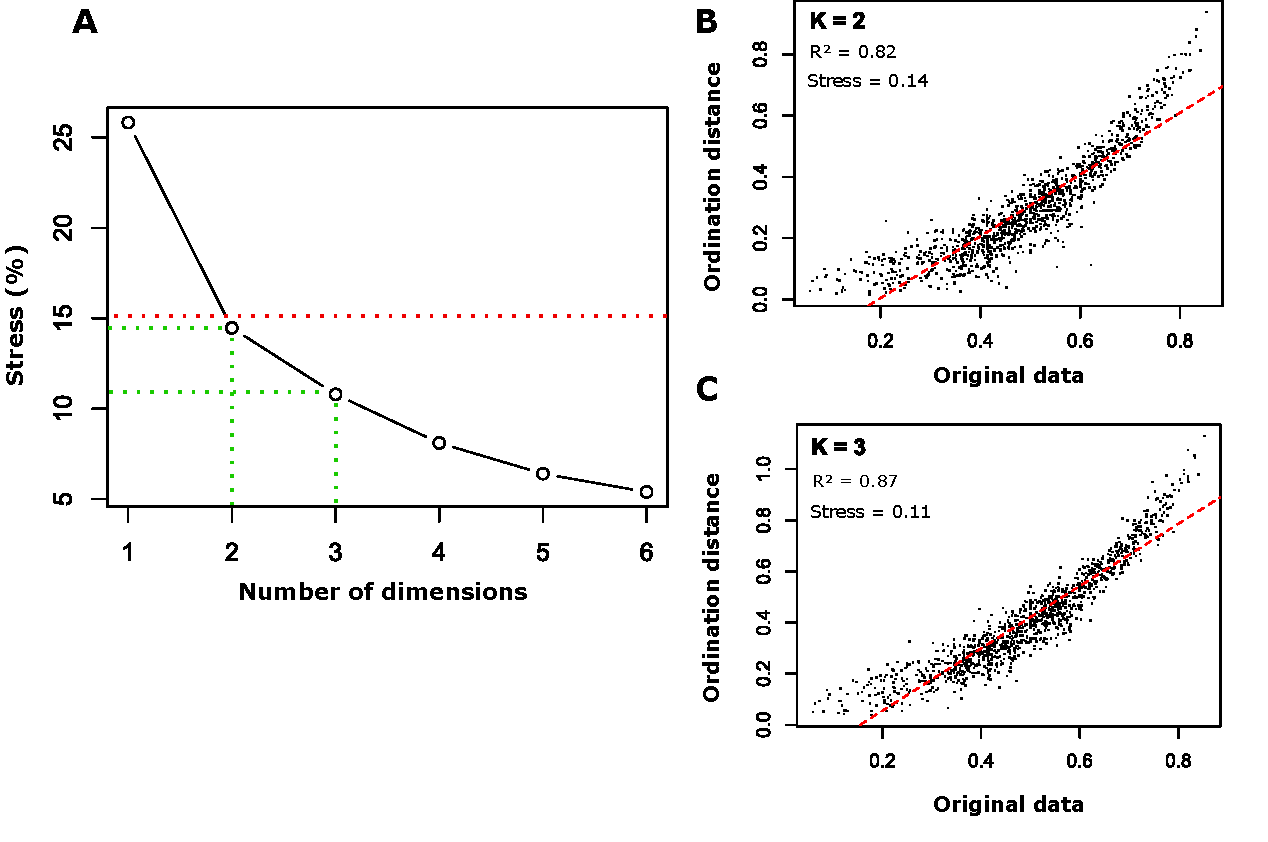
\includegraphics[scale =0.9]{Images/scree_and_shepard_plots.pdf}
	\caption{A) Scree plot showing the relationship between the number of dimensions used for a non-metric MDS, and the corresponding stress score. Stress scores below 15\% are considered to be a good fit for the data (indicated by the dashed red line). Stress scores for K = 2 and K = 3 are indicated by the dashed green lines. Shepard plots are shown in B) (K = 2) and C) (K = 3), plotting the relationship between the original distance data and the distances resulting from the ordination transformation. A high R\textsuperscript{2} value is desirable, as that indicates an accurate reflection of the data in the ordination plot.} 
	\label{fig:shep_plots}
\end{figure}
\end{landscape}

% \subsection{Structure results}
% \begin{figure}[H]
% 	\centering
% 	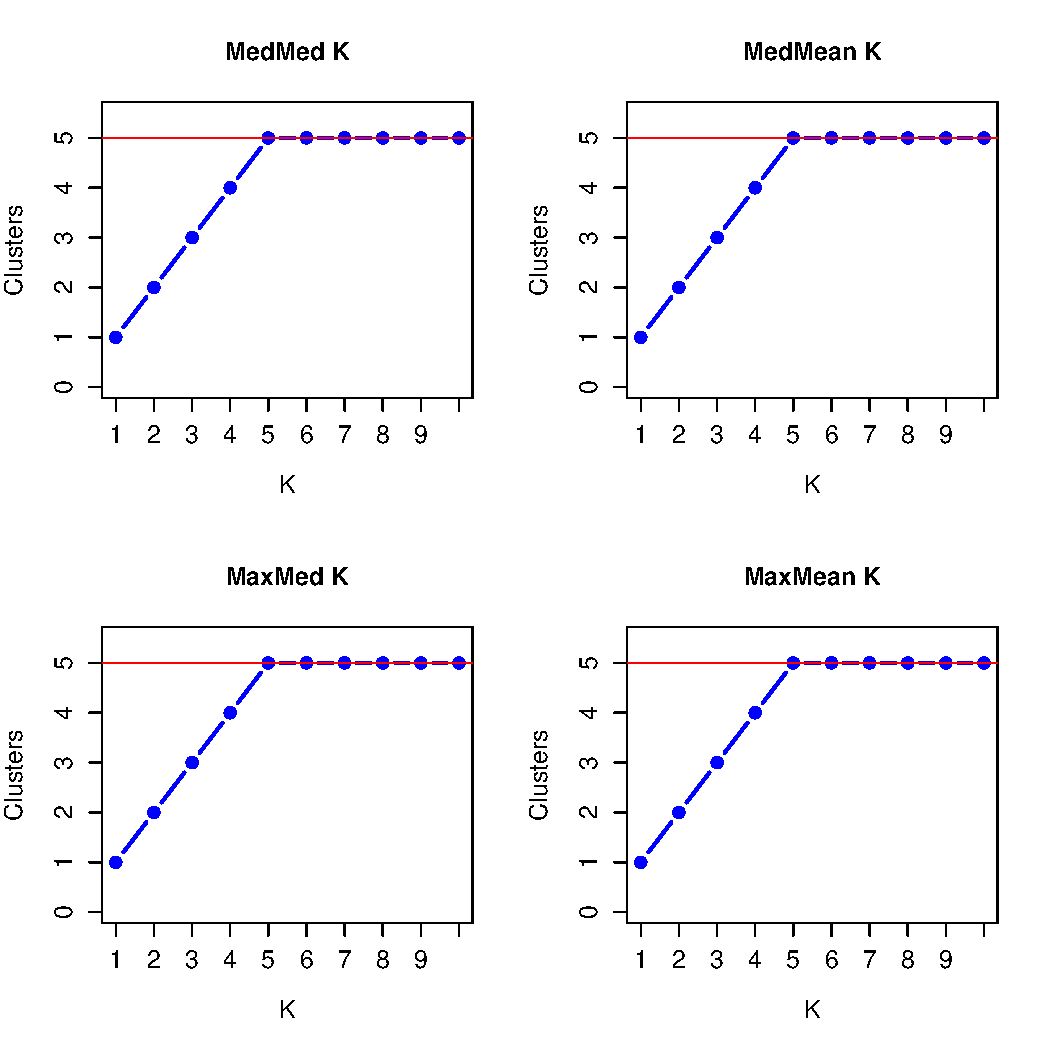
\includegraphics[scale =0.7]{Images/MedK_0,7_without_priors.pdf}
% 	\caption{Estimation of the optimal \textit{K}-value (\textit{K} = 5) according to the four methods presented by \citet{puechmaille2016program}. The threshold value presented above was set to 0.6. (PopData was not set as a prior).}
% 	\label{fig:struc_thresh0.6}
% \end{figure}

% \begin{figure}[H]
% 	\centering
% 	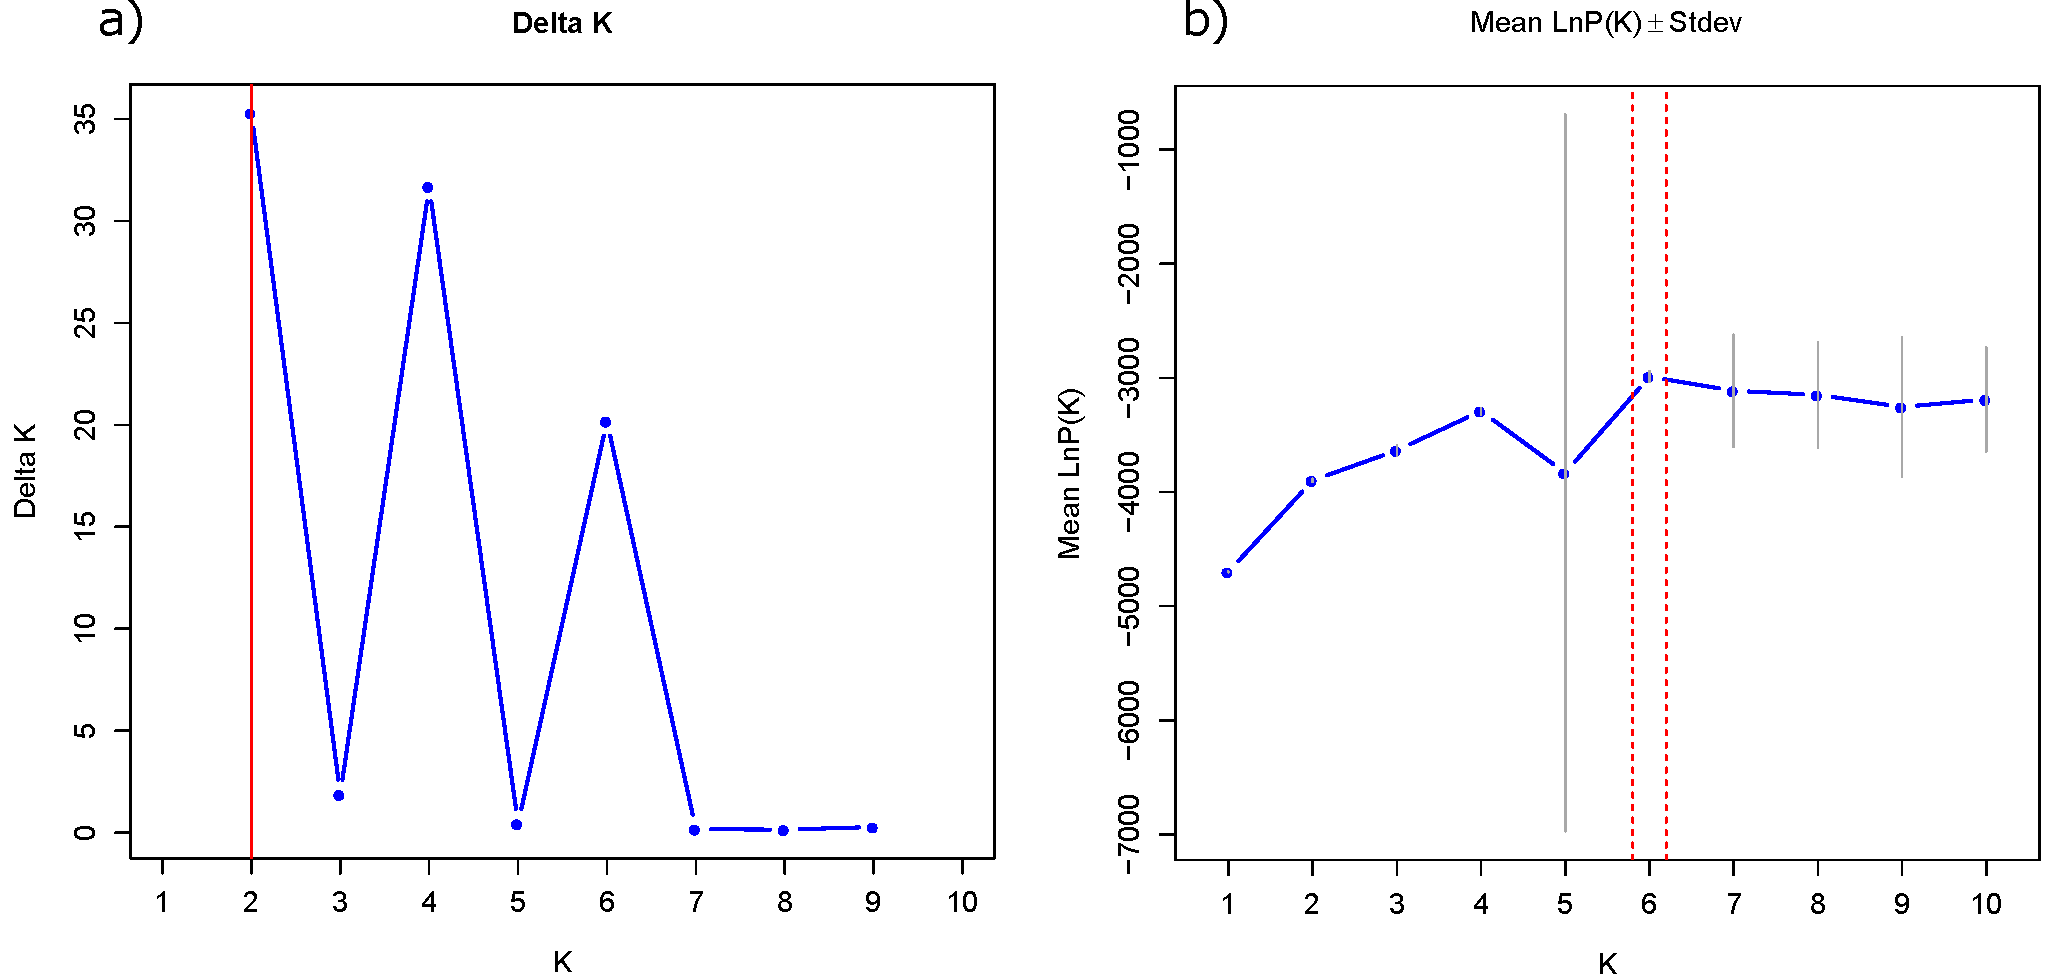
\includegraphics[scale =0.45]{Images/DeltaK_LnPK_without_priors.pdf}
% 	\caption{Estimation of the optimal \textit{K}-value, using a) $\Delta$\textit{K} and b) the mean LnP(\textit{K}) estimates as per the methods of \citet{evanno2005detecting}. (PopData was not set as a prior).}
% 	\label{fig:struc_evanno}
% \end{figure}

% \begin{figure}[H]
% 	\centering
% 	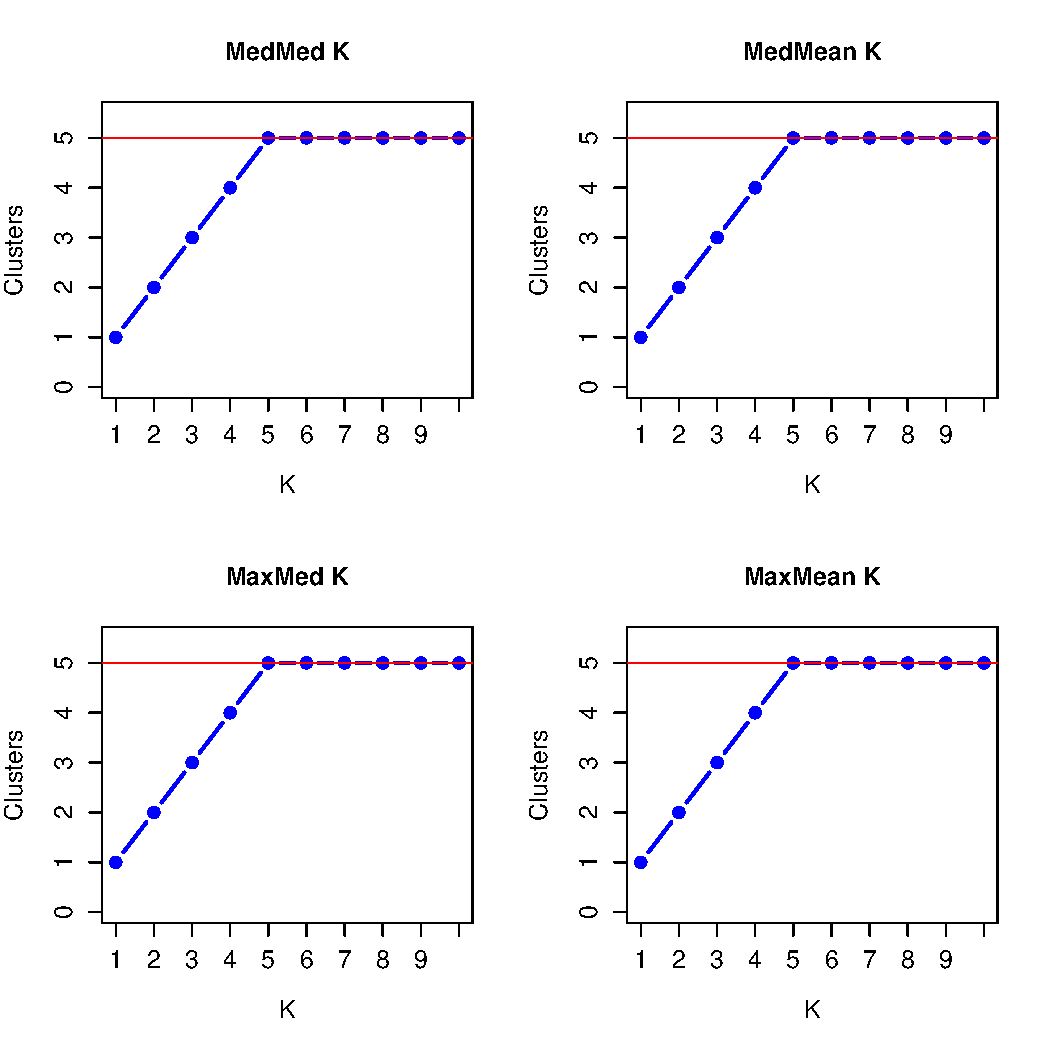
\includegraphics[scale =0.7]{Images/with_priors_structure_medK_graphs.pdf}
% 	\caption{Estimation of the optimal \textit{K}-value (\textit{K} = 5) according to the four methods presented by \citet{puechmaille2016program}. The threshold value presented above was set to 0.7. PopData set as a prior.}
% 	\label{fig:struc_K_locprior_puech}
% \end{figure}

% \begin{figure}[H]
% 	\centering
% 	\includegraphics[scale =0.45]{Images/DeltaK_LnPK.pdf}
% 	\caption{Estimation of the optimal \textit{K}-value, using a) $\Delta$\textit{K} and b) the mean LnP(\textit{K}) estimates as per the methods of \citet{evanno2005detecting}. PopData set as a prior.}
% 	\label{fig:struc_locprior_evanno}
% \end{figure}

\subsection{ISSR primer statistics}
\begin{table}[H]
\caption{POPGENE statistical output for each individual primer and their concatenation for the `stricta' and `ficus' genetic clusters. na = number of alleles, ne = effective number of alleles, h = Nei's genetic diversity, I = Shannon's information index, No. PM loci = number of polymorphic loci, \% PM loci = percentage polymorphic loci, Ht = total genetic diversity, Hs = intra population genetic diversity,  Gst = coefficient of gene differentiaion. All values presented are averages. For the intra-group statistics, Saudi Arabia + Kruger N. Park + Klein \& Hoffmann = `stricta', and Uitenhage + Namibia + wild populations = `ficus'.}
\label{tab:issr_stats_eachPrimer}
\renewcommand{\arraystretch}{0.5}
\resizebox{\columnwidth}{!}{
\begin{tabular}{@{}llcccccclll@{}}
\toprule
\textbf{Primer} & \textbf{Group} & \textbf{na} & \textbf{ne} & \textbf{h} & \textbf{I} & \textbf{No. PM loci} & \textbf{\%  PM loci} & \textbf{Ht} & \textbf{Hs} & \textbf{Gst} \\ \midrule
\textbf{ISSR 809} & stricta & 1.20 & 1.09 & 0.06 & 0.09 & 78 & 20.31 & 0.06 & 0.03 & 0.51 \\
 & ficus & 1.41 & 1.17 & 0.11 & 0.17 & 156 & 40.62 & 0.14 & 0.06 & 0.59 \\
 & Mass Rearing Facility & 1.19 & 1.14 & 0.08 & 0.11 & 74 & 19.27 &  &  &  \\
 & All & 1.45 & 1.15 & 0.10 & 0.16 & 174 & 45.31 & 0.13 & 0.10 & 0.23 \\
 & \textbf{INTRA-GROUP:} &  &  &  &  &  &  &  &  &  \\
 & Saudi Arabia & 1.08 & 1.05 & 0.03 & 0.04 & 30 & 7.81 &  &  &  \\
 & Kruger N. Park & 1.09 & 1.06 & 0.03 & 0.05 & 35 & 9.11 &  &  &  \\
 & Klein \& Hoffmann & 1.07 & 1.05 & 0.03 & 0.04 & 27 & 7.03 &  &  &  \\
 & Uitenhage & 1.15 & 1.13 & 0.07 & 0.10 & 56 & 14.58 &  &  &  \\
 & Namibia & 1.12 & 1.11 & 0.06 & 0.08 & 47 & 12.24 &  &  &  \\
 & Wild populations & 1.15 & 1.08 & 0.05 & 0.07 & 58 & 15.1 &  &  &  \\
\textbf{ISSR 826} & stricta & 1.03 & 1.03 & 0.01 & 0.02 & 11 & 3.01 & & & \\
 & ficus & 1.03 & 1.03 & 0.02 & 0.02 & 12 & 3.28 & & &  \\
 & stricta + ficus & 1.06 & 1.04 & 0.03 & 0.04 & 23 & 6.28 & & &  \\ 

 \bottomrule
\end{tabular}
}
\end{table}

% \subsection{POPGENE file input}
% \label{appendix:popgene_input}

% The POPGENE input file followed the following format, where a `.' indicates missing or ambiguous data: \newline

% \noindent /*ISSRpopgene*/ \\
% Number of populations = 2 \\
% Number of loci = 6 \\
% locus name: \\
% Locus 1 Locus 2 Locus 3 Locus 4 Locus 5 Locus 6\\

% \noindent name = population1 \\
% 001110 \\
% 001110 \\
% 0110.0 \\
% 11001. \\

% \noindent name = population2 \\
% 0.0111 \\
% 010111 \\
% 0.1110 \\
% 1110.1 \\

\subsection{Genetic distance and diversity}
All \textit{D. opuntiae} specimens showed an average Jaccard distance of 0.48 (SE $\pm$ 0.01) (Fig. \ref{fig:genetic_distances_boxplot}). None of the within-group genetic distances showed significant differences (Kruskal-Wallis ANOVA: Fig. \ref{fig:genetic_distances_boxplot}A)  Chi-square = 2.84, p= 0.24, and Fig. \ref{fig:genetic_distances_boxplot}B) Chi-square = 6.72, p= 0.081).
By group, `ficus' had the highest percentage of polymorphic loci (PM) (38.53 \%), as well as genetic diversity (h = 0.10, I = 0.16), while samples from the MRF had the lowest percentage PM loci (17.33 \%) (Table \ref{tab:popgene_stats}). \\

\begin{figure}[H]
	\centering
	\includegraphics[scale =0.75]{Images/genetic_distances_boxplot.pdf}
	\caption{Box plots for within and overall group genetic distances for \textit{D. opuntiae}, measured by the Jaccard distance (1-J). A) `ficus' taken as a whole and B) wild populations removed from `ficus' and put into its own group. Solid black dots are the means, and the same letters above each box indicate non-significance.}
	\label{fig:genetic_distances_boxplot}
\end{figure}

% At the intra-group level, wild populations (`ficus') had the highest percentage PM loci (14.8\%), and the Hoffmann and Klein `stricta' source populations had the lowest (6.67\%) (Table \ref{tab:popgene_stats}). \\
% The largest genetic distances were between Namibian `ficus' and 1) the Hoffmann and Klein `stricta' source populations (0.189), 2) Kruger National Park `stricta' (0.177), 3) wild population `ficus' (0.173) and 4) Saudi Arabian `stricta' samples (0.168) (Table \ref{tab:popgene_genetic_distances}). 
 
\begin{table}[H]
\renewcommand{\arraystretch}{0.5}
\caption{POPGENE statistical output for the concatenation of ISSR 809 and ISSR 826 for the `stricta' and `ficus' genetic clusters. na = number of alleles, ne = effective number of alleles, h = Nei's genetic diversity, I = Shannon's information index, No. PM loci = number of polymorphic loci, \% PM loci = percentage polymorphic loci, Ht = total genetic diversity, Hs = intra population genetic diversity,  Gst = coefficient of gene differentiaion. All values presented are averages. For the intra-group statistics, Saudi Arabia + Kruger N. Park + Klein \& Hoffmann = `stricta', and Uitenhage + Namibia + wild populations = `ficus'.}
\label{tab:popgene_stats}
\resizebox{\columnwidth}{!}{
\begin{tabular}{@{}llcccccclll@{}}
\toprule
\textbf{Primer} & \textbf{Group} & \textbf{na} & \textbf{ne} & \textbf{h} & \textbf{I} & \textbf{No. PM loci} & \textbf{\%  PM loci} & \textbf{Ht} & \textbf{Hs} & \textbf{Gst} \\ \midrule
 \textbf{ISSR 809 \& ISSR 826} & stricta & 1.22 & 1.10 & 0.06 & 0.10 & 165 & 22 & 0.06 & 0.03 & 0.48 \\
 & ficus & 1.39 & 1.16 & 0.10 & 0.16 & 289 & 38.53 & 0.14 & 0.05 & 0.63 \\
 & Mass Rearing Facility & 1.17 & 1.13 & 0.07 & 0.10 & 130 & 17.33 & & & \\
 & All & 1.45 & 1.15 & 0.10 & 0.16 & 337 & 44.93 & 0.12 & 0.10 & 0.21 \\
 & \textbf{INTRA-GROUP:} &  &  &  &  &  &  & & &  \\
 & Saudi Arabia & 1.07 & 1.05 & 0.03 & 0.04 & 55 & 7.33 & & &  \\
 & Kruger N. Park & 1.13 & 1.07 & 0.04 & 0.07 & 98 & 13.07 & & &  \\
 & Klein \& Hoffmann & 1.07 & 1.05 & 0.03 & 0.04 & 50 & 6.67 & & &  \\
 & Uitenhage & 1.10 & 1.09 & 0.05 & 0.07 & 78 & 10.40 & & &  \\
 & Namibia & 1.12 & 1.10 & 0.05 & 0.08 & 86 & 11.47 & & &  \\
 & Wild populations & 1.15 & 1.08 & 0.05 & 0.07 & 111 & 14.8 & & &  \\
 \bottomrule
\end{tabular}
}
\end{table}

% \subsection*{Scanning Electron Microscope images}
% \label{appendix:semImages}

% \begin{landscape}
% \begin{figure}[H]
% 	\centering
% 	\includegraphics[scale =0.5]{Images/dactylopius_austrinus.pdf}
% 	\caption{} 
% 	\label{}
% \end{figure}
% \end{landscape}

% \begin{landscape}
% \begin{figure}[H]
% 	\centering
% 	\includegraphics[scale =0.5]{Images/dactylopius_ceylonicus.pdf}
% 	\caption{} 
% 	\label{}
% \end{figure}
% \end{landscape}

% \begin{figure}[H]
% 	\centering
% 	\includegraphics[scale =0.5]{Images/dactylopius_opuntiae_ficus.pdf}
% 	\caption{} 
% 	\label{}
% \end{figure}

% \begin{figure}[H]
% 	\centering
% 	\includegraphics[scale =0.6]{Images/dactylopius_tomentosus_cholla.pdf}
% 	\caption{} 
% 	\label{}
% \end{figure}

% \begin{landscape}
% \begin{figure}[H]
% 	\centering
% 	\includegraphics[scale =0.5]{Images/dactylopius_tomentosus_imbricata.pdf}
% 	\caption{} 
% 	\label{}
% \end{figure}
% \end{landscape}

\section{R Scripts}
\label{appendix:rScripts}

\subsection{Barcode testing using SPIDER}
\label{appendix:RCODE,SPIDER}
% \textbf{R code for the basic barcode testing algorithms in the Spider package, adapted from the tutorial by \citet{Brown2012Spider:Barcoding}} \\

\begin{lstlisting}[language=R]
# Read in a .fas file
setwd("file_location")
getwd()
input = "file_name.fas"
seqs = read.dna(input, format = 'fas')
dist = dist.dna(seqs, pairwise.deletion = TRUE)
# Nearest neighbour:
sppNames = dimnames(seqs)
table(nearNeighbour(dist, sppNames))
# Threshold Identification:
table(threshID(dist, sppNames, threshold = 0.01))
# Meier's Best Close Match:
table(bestCloseMatch(dist, sppNames, threshold = 0.01))
# Optimising the threshold value from the default of 0.01:
threshVal = seq(0.001,0.02, by = 0.001)
sens = lapply(threshVal, function(x) threshOpt(dist, sppNames, thresh = x))
sensMat = do.call(rbind, sens)
barplot(t(sensMat)[4:5,], names.arg=paste((sensMat[,1]*100), "%"))
# Graphically displaying the barcoding gap:
inter = nonConDist(dist, sppNames) *100
intra = maxInDist(dist, sppNames) *100
bnd = cbind(data.frame(inter, intra))
ord = bnd[order(bnd$inter),]
plot(ord$inter, type="n", ylab="Percent K2P distance", xlab="Individual")
segCol = rep("gray50", length(ord$inter))
segCol[ord$inter-ord$intra < 0] = "red" 
segments(x0=1:length(ord$inter), y0=ord$inter, y1=ord$intra, col=segCol, lwd=6)
\end{lstlisting}

\subsection{Jaccard's transformation}
% Jaccard's transformation was applied in R using the `dist' function with the `binary' method using the following code: \newline
\label{appendix:RCODE,Jaccard}
\begin{lstlisting}[language=R]
binarymat <-read.csv("file_name.csv", header = T, sep = ",", dec = ".")
# removes the first two columns, which contain sample names and grouping information
binarymat2 = binarymat[,c(-1,-2)] 
# assign sample names as row names 
row.names(binarymat2) = binarymat[,1] 
# shortens the names to 10 characters
newnames =substring(row.names(binarymat2), 0, 10) 
row.names(binarymat2) = newnames
# replaces ? with NA, as NA's are ignored.
binarymat2[binarymat2=="?"] <- NA 
# converts the matrix to a data frame 
binarymat2 = as.data.frame(binarymat2) 
# creates a distance matrix
d = dist((binarymat2), method = "binary", diag = TRUE, upper = T) 
d = as.data.frame(as.matrix(d))
d2 =  as.dist(d)

\end{lstlisting}

\subsection{UPGMA clustering tree}
\label{appendix:RCODE,upgma}
\begin{lstlisting}[language=R]
library(pvclust)
# 'average' refers to the UPGMA method. 
# binarymat2 is transformed such that the data is organised by column.
result <- pvclust(t(binarymat2), method.dist = "binary", method.hclust="average", nboot=1000) 
p = plot(result, cex = 0.6, print.num = F, print.pv = T, cex.pv = 0.6)

\end{lstlisting}

\subsection{Non-metric MDS plot}
\label{appendix:RCODE, nmds}
\begin{lstlisting}[language=R]
# k is the number of dimensions
# d2 is the distance matrix obtained for the data using the `binary' method
fit <- isoMDS(d2, k=2) 
# view the stress value
fit$stress 
mds_plot = isoMDS(d2,k=2)
eqscplot(mds_plot$points, col = c("red", "dodgerblue3", "forestgreen", "orange")[binarymat$Group], pch = c(15, 16, 17,18)[binmat$Group])
# the number of colours and pch types selected will depend on the number of groups (binarymat$Group) inputted
scree.plot = function(d, k) {
stresses=isoMDS(d, k=k)$stress
  for(i in rev(seq(k-1)))  
  stresses=append(stresses,isoMDS(d, k=i)$stress)
  plot(seq(k),rev(stresses), type="b", xaxp=c(1,k, k-1), ylab="Stress", xlab="Number of dimensions")
}
# plot stress values for six dimensions
scree.plot(d2, k=6) 
shep<-Shepard(d2, mds_plot$points, p=2)
plot(shep, pch=".", main = "K = 2")
# R squared value
summary(lm(shep$y~shep$x)) 
# line of best fit through the points
abline(lm(shep$y~shep$x), col = "red", lty = 2) 
\end{lstlisting}

\subsection{Three dimensional non-metric MDS plot}
Although not included in the results, three dimensional nMDS (Non-metric Multidimensional Scaling) scatter plots were created in R using the plot3D package \citep{Soetaert}. The following following code was implemented: \newline

\begin{lstlisting}[language=R]
# nMDS with three dimensions
fit <- isoMDS(d2, k=3) 
x <- fit$points[,1]
y <- fit$points[,2]
z <- fit$points[,3]
library(plot3D)
# points are coloured by group, which was column 2 in the original binarymat matrix
scatter3D(x,y,z, phi = 25,  type = "h", 
pch = 19, cex = 1.5, bty = "b", colvar = as.integer(binarymat$Group), col = c("blue", "red"), colkey = list(side = 2, length = 0.5))
# an optional addition to add sample names above points in the scatter plot
text3D(x, y, z, labels = rownames(binarymat2), add = TRUE, colkey = FALSE, cex = 0.7) 
\end{lstlisting}

\subsection{ANOSIM and PERMANOVA}
\label{appendix:RCODE,anosim,permanova}
\begin{lstlisting}[language=R]
# ANOSIM:
anosim(d2, binarymat$Group, permutations = 999, distance = "jaccard")
# PERMANOVA:
library(vegan)
adonis(d2~binarymat$Group)
library(RVAideMemoire)
pairwise.perm.manova(d2, binarymat$Group)
\end{lstlisting}


\begin{landscape}
\section{Shiny Applications}
\begin{figure}[H]
	\centering
	\includegraphics[scale = 0.42]{Images/barcode_tester_gui.pdf}
    \newline
	\caption{Genetic barcode tester GUI showing the components of the application. Numbers in circles indicate the order in which data is uploaded and processed.}. 
	\label{fig:barcodeTesterGUI}
\end{figure}
\end{landscape}

\begin{landscape}
\begin{figure}[H]
	\centering
	\includegraphics[scale = 0.45]{Images/binmat_gui.pdf}
    \newline
	\caption{Binary matrix processing application (`BINMAT'), where the user uploads a .csv file containing binary data replicates in order to consolidate them. Summary statistics, error rates and the construction of a UPGMA clustering tree are also available. Non-metric MDS plots can be created by uploading a consolidated binary matrix, where filtering of samples with a low peak count can be applied.} 
	\label{fig:binmatGUI}
\end{figure}
\end{landscape}

\subsection{Dacty-ID}

When uploading this application to the Shiny server, the following command was required in R in order to set the repositories to access packages within Bioconductor (namely the DECIPHER package by \citet{wright2016using}): \\ \\
\noindent
\texttt{
setRepositories() \\
} \\
\noindent This produced the output on the console: \\ \\
\texttt{
\noindent 1: + CRAN \\
2:   BioC software \\
3:   BioC annotation \\
4:   BioC experiment \\
5:   CRAN (extras) \\
6:   Omegahat \\
7:   R-Forge \\
8:   rforge.net \\
Enter one or more numbers separated by spaces, or an empty line to cancel \\
1: } \\

\noindent Options 2, 3, and 4 were entered to include all the BioC-related dependencies.

\begin{landscape}
\begin{figure}[H]
	\centering
	\includegraphics[scale = 0.4]{Images/dactylopius_identifier_GUI.pdf}
	\caption{Identification GUI application, where the user can test the identity of a query sequence against a preselected genetic database. A phylogenetic tree is displayed on the screen, with the position of the query sequence highlighted in red.}
	\label{fig:identifier_GUI}
\end{figure}
\end{landscape}

\section{MRBAYES Nexus files}
\label{appendix:bayesblocks}

\subsection{12S}
\fbox{\parbox{\textwidth}{%
{\parindent0pt %

\#NEXUS \\
{[12S aligned sequences]} \\

begin data; \\
dimensions ntax=152 nchar=779; \\
format interleave datatype=DNA missing=N gap=-; \\

matrix \\
ALIGNED 12S SEQUENCES \\
; \\
end; \\

begin mrbayes; \\
	set autoclose=yes nowarn=yes; \\
	lset nst=6 rates=gamma ngammacat = 4 code=universal; \\
	outgroup HQ893819.1; \\
	prset revmatpr = dirichlet(6.0485, 8.2345, 15.0465, 0.0004, 42.1397, 1.0000) \\
	statefreqpr = dirichlet(0.3923, 0.1404, 0.1629, 0.3044) \\
	shapepr = fixed(0.8960); \\
	mcmc Ngen=50000000 printfreq=1000 samplefreq=1000 Nchains=4 savebrlens=yes starttree=random; \\
	sumt burnin = 1250; \\
	sump burnin = 1250; 
  
end; \\

}%
}} %

\subsection{18S}

\fbox{\parbox{\textwidth}{%
{\parindent0pt %

\#NEXUS \\
{[18S aligned sequences]} \\

begin data; \\
dimensions ntax=153 nchar=630; \\
format interleave datatype=DNA missing=N gap=-; \\

matrix \\
ALIGNED 18S SEQUENCES \\
; \\
end; \\

begin mrbayes; \\
set autoclose=yes nowarn=yes; \\
	lset nst=6 rates=propinv ngammacat = 4 code=universal; \\
	outgroup KY9276001; \\
	prset revmatpr = dirichlet(0.5109, 1.8724, 0.5109, 1.0000, 3.5607, 1.0000) \\
	pinvarpr = fixed(0.6060); \\
	mcmc Ngen=50000000 printfreq=1000 samplefreq=1000 Nchains=4 savebrlens=yes starttree=random; \\
	sumt burnin = 1250; \\
	sump burnin = 1250; \\
  
end; 

}%
}} %

\subsection{COI}

\fbox{\parbox{\textwidth}{%
{\parindent0pt %

\#NEXUS \\
{[COI aligned sequences]} \\

begin data; \\
dimensions ntax=97 nchar=603; \\
format interleave datatype=DNA missing=N gap=-; \\

matrix \\
ALIGNED COI SEQUENCES \\
; \\
end; \\

begin mrbayes; \\

	set autoclose=yes nowarn=yes; \\
	lset nst=2 rates= gamma ngammacat = 4 code=universal; \\
	outgroup AB440072.2; \\
	prset statefreqpr = dirichlet(0.3872, 0.1822,  0.0454, 0.3853) \\
	shapepr = fixed(0.6260) tratiopr = fixed(2.1838); \\
	mcmc Ngen=50000000 printfreq=1000 samplefreq=1000 Nchains=4 savebrlens=yes starttree=random; \\
	sumt burnin = 1250; \\
	sump burnin = 1250; \\
  
end; 

}%
}} %


% \subsection{DTOMf \& HCO2198}

% \fbox{\parbox{\textwidth}{%
% {\parindent0pt %

% \#NEXUS \\
% {[DTOMf aligned sequences]} \\

% begin data; \\
% dimensions ntax=24 nchar=574; \\
% format interleave datatype=DNA missing=N gap=-; \\

% matrix \\
% ALIGNED DTOMf \& HCO2198 SEQUENCES \\
% ; \\
% end; \\

% begin mrbayes; \\

% set autoclose=yes nowarn=yes; \\
% 	lset nst=6 rates=gamma ngammacat=4 code=universal; \\
% 	outgroup CVS154\_COI; \\
% 	prset revmatpr=dirichlet(1.0000,2.7143,1.0000,1.0000,12.2861,1.0000) \\ statefreqpr=dirichlet(0.3613,0.2002,0.0584,0.3801) \\
% 	shapepr=fixed(0.2940); \\
% 	mcmc Ngen=50000000 printfreq=1000 samplefreq=1000 Nchains=4 savebrlens=yes starttree=random; \\ 
% 	sumt burnin=1250; \\
% 	sump burnin=1250; \\
  
% end; 

% }%
% }} %

% \section{Costs}
% Nucleotide sequencing and ISSR fragment analysis costs approximately R 155.08 (US\$10.06) and R 90.34 (US\$5.86) per sample, respectively, at 2019 prices. Taking the replication of ISSR samples into account, the cost per sample is approximately R 155.37 (US\$10.08).
\renewcommand{\chaptername}{}

\setcounter{table}{0}
\renewcommand{\thetable}{B\arabic{table}}

\setcounter{figure}{0}
\renewcommand{\thefigure}{B\arabic{figure}}

\chapter{Appendix B: Additional literature review material} 
\label{sec:appendix2}

In their hybrid study of \textit{Dactylopius tomentosus} lineages, \citet{Mathenge2010} postulated that male and female crawlers might display differing host specifities due to the Comstockiella genetic system displayed in this insect family. In other words, males are haploid, containing only a maternal genome, while females are diploid with both a maternal and paternal genome. Taking such underlying genetic processes into account may be useful in explaining observed trends in inherited traits and the resulting host-specificity displayed by hybrid offspring. 

\section{The genetic system of the scale insects}
\label{appendix:geneticSystem}
The scale insects display one of the most diverse genetic and sex-determination systems of all the insects, including diploidy, parthenogenesis, hermaphroditism and haplodiploidy \citep{Burt2009,Ross2012}. The ancestral genetic system of scale insects is that of XX-XO (where 2n = 10), such that females are homogametic, and males are heterogametic with only one sex chromosome \citep{Hughes-Schrader1948, Nur}. 
Arrhenotoky and paternal genome elimination (PGE) (also termed ‘pseudoarrhenotoky’ or ‘parahaplodiploidy’) are variants of the haplodiploidy genetic system \citep{Haig1993,Gullan1997, Normark2004, Burt2009, Ross2010GenomicSystems}. To further complicate matters, the Hemiptera possess holocentric chromosomes, where spindle fibres attach along the length of the chromosome during cell division \citep{Hughes-Schrader1948}. This is in contrast to the typical monocentric chromosomes where spindle fibres attach to a single centromere \citep{Melters2012}. Holocentric chromosomes have allowed for a diverse range of karyotypes to form within the scale insects, such as species in the \textit{Apiomorpha} genus (Coccoidea: Eriococcidae) that display chromosome numbers from 2N = 4 to 2N = 92 \citep{Cook2000}. This is because if holocentric chromosomes become fragmented, all segments are pulled to opposite poles of the cell by spindle fibres during meiosis, as opposed to monocentric chromosomes that do not include fragmented sections and thereby maintain their original karyotype \citep{Melters2012}.  Additionally, scale insects display inverse meiosis \citep{Hughes-Schrader1948, Chandra1962, Bongiorni2004}. In this process, equational division occurs first followed by reduction division \citep{Wrensch1994, Bongiorni2004}. The difference between normal and inverse meiosis comes about due to the position of the paternal and maternal chromosomes relative to the orientation of the spindle fibres that form prior to metaphase I \citep{Wrensch1994} (Figure \ref{fig:meiosis}).

\vspace{1cm}

\begin{figure}[H]
	\centering
	\includegraphics[scale = 0.6]{Images/meiosis.pdf}
	\caption{Difference between normal and inverted meiosis. Adapted from \citet{Brown1964, Wrensch1994, Bongiorni2004}}
	\label{fig:meiosis}
\end{figure} 

\subsection{The evolution of haplodiploidy}
Haplodiploidy refers to a genetic system where males are haploid and contain only a maternal genome, and females are diploid with both a maternal and paternal genome \citep{Normark2004, DelaFilia2015}. Haploidy in males occurs through either arrhenotoky (where females produce male offspring parthenogenetically) or PGE (where the paternal genome is eliminated at different developmental stages) \citep{Bull1979, Burt2009, Ross2010GenomicSystems}.
Haplodiploidy is present in as many as 15\% of arthropods \citep{DelaFilia2015}, and has evolved at least 10 times in insects \citep{Normark2004, Normark2006}. Why this system evolved is not well understood, but the leading hypotheses suggest the antagonistic co-evolution (intragenomic conflict) between the sexes, conflict over sex-determination, the clearance of deleterious mutations and rapid adaptation, and the role of endosymbionts (intergenomic conflict) in determining chromosome dynamics are possible drivers \citep{Normark2004, Burt2009, Ross2010GenomicSystems, DelaFilia2015}. 
\citet{Bull1979} and \citet{Herrick1999} suggested that maternal and paternal chromosomes engage in an arms race during spermatogenesis to transmit their genes to the next generation, and that this may explain the evolution of the different variations of PGE in scale insects. Females that produce haploid sons increase the transferal of their genes by two-fold in the gametes that their sons will produce \citep{Bull1979}. \citet{Normark2006} suggested that if an insect group displays gregariousness (as scale insects do), maternal care or other close kin associations, and relatedness asymmetry (i.e. offspring are linked more closely through their maternal line than through paternal genes), then offspring are more likely to display cooperative rather than competitive behaviour towards each other. In this case, some male genes may pose as selfish elements and can decrease overall fitness. \\
The sex determination system of scale insects that display PGE is poorly understood, with no record of the observation of sex chromosomes in species with this genetic system \citep{Brown1964, Ross2010GenomicSystems}. It is hypothesised that sex is determined by mechanisms such as gamete imprinting, the addition of maternal proteins to eggs \citep{Ross2010GenomicSystems}, the activity of endosymbionts \citep{Buchner1965}, and factors such as temperature \citep{Nelson-Rees1962}, population density, and the age of females at mating and oviposition \citep{Ross2010b}. Studies by \citet{Sabour1972} and \citet{Bongiorni2007} suggest that PGE and sex determination are maternally controlled through the production of histone proteins such as HP1, while \citet{Buglia2004} propose that it is the sperm that are tagged with proteins that determine sex. As an extension of intragenomic conflict between the sexes, haplodiploid fathers may favour a female-biased sex ratio, as this will ensure the transmittance of their genes to offspring \citep{DelaFilia2015}. This may lead to male selection for the manipulation of PGE dynamics \citep{DelaFilia2015}. Contrastingly, females may favour a male-biased sex ratio due to resource competition between daughters \citep{Taylor1981}. Since female scale insects are sessile and longer-lived in contrast to short-lived mobile males, females require more resources for survival and reproduction \citep{Taylor1981, Ross2010b}. \citet{Ross2010GenomicSystems}, for example, showed that \textit{Planococcus citri} (Coccoidea: Pseudococcidae) facultatively adjusted the sex ratio of offspring to favour males in response to high population densities. \\
Mutation rates and the efficiency of selection differentially affects haploid and diploid organisms \citep{Otto2008}. Relatively more mutations occur in diploids than haploids due to there being twice the number of genes available \citep{Mable1998, Otto2008, DelaFilia2015}. However, because of the capacity of homologous chromosome pairs to display heterozygosity, beneficial recessive mutations are masked and may take longer to become expressed in diploids \citep{Mable1998}. Additionally, the elimination of deleterious mutations through selection may be delayed due to this property \citep{Otto2008}. Because haploids immediately express mutations, deleterious mutations may be eliminated more efficiently, and beneficial mutations can spread more quickly through a haploid population \citep{DelaFilia2015}. Since haploid cells are generally smaller than diploid cells \citep{Galitski1999}, haploids have a higher surface area to volume ratio. It has therefore been suggested that haploid organisms have the ability to take in more nutrients across their cell membranes and have a higher chance of survival under nutrient-limited conditions \citep{Lewis1985}. Additionally, a smaller genome size could be less metabolically demanding \citep{Lewis1985}. \citet{Cavalier-Smith1978} suggested that smaller-bodied organisms, such as many endoparasites, tend to display haplodiploidy while larger-bodied organisms tend to be diploid due to differences in cell volume. \\
Scale insects feed on the phloem of their host plants, which is typically sugar-rich but nitrogen-poor \citep{Buchner1965, Douglas2006}. This has led to the evolution of obligate symbiotic relationships with microorganisms such as bacteria and unicellular fungi that synthesise amino acids and vitamins that their hosts can utilise \citep{Buchner1965,Douglas1998, Douglas2006, Douglas2015}. Endosymbiotic bacteria are usually housed in specialized organs called ‘bacteriomes’, in haemolymph, or inside modified fat cells within the insect host’s body \citep{Buchner1965, Normark2004b, Rosenblueth2018}. Bacteria are vertically transmitted to offspring via the maternal line in the cytoplasm of eggs \citep{Buchner1965, Rosenblueth2018}. Since males play no role in the transferal of bacteriomes, it is theorized that a potential intergenomic conflict exists between male hosts and endosymbionts regarding sex allocation \citep{Ross2010GenomicSystems}. Bacteria would favour a female-biased ratio to ensure their survival, while male insects would resist this pressure to prevent a reduction in paternal gene transfer to offspring \citep{Ross2010GenomicSystems}. In PGE systems however, male hosts and endosymbionts may have a shared interest in a female-biased sex ratio as males can only transmit their genes to female offspring, as discussed above \citep{Ross2010GenomicSystems}. Some studies have shown that symbionts can feminise \citep{Rigaud1997} and even kill males \citep{Hurst1991}, or induce parthenogenesis in their host \citep{Stouthamer1990}. 

\subsection{Paternal genome elimination}
Paternal genome elimination involves the deactivation and elimination of the paternal half of the genome through the process of heterochromatisation in male offspring \citep{Nur, Ross2010GenomicSystems}. As such, male sons transmit only their mother's genome to the next generation, making their closest male relatives their maternal grandfathers \citep{DelaFilia2015}. In this way, selection on male genes skips a generation \citep{DelaFilia2015}. At least 20 000 recorded species display PGE \citep{DelaFilia2015}, including more than half of the approximately 6000 known species of scale insects \citep{Burt2009}. It has also been recorded in some fungus gnats (\textit{Sciara} spp.) \citep{Haig1993b}, gall midges (\textit{Mayetiola destructor}) \citep{Haig1993}, phytoseiid mites (\textit{Amblyseius} spp.) \citep{Nelson-Rees1980}, springtails (\textit{Sminthurus viridis} and \textit{Allacma fusca}) (Collembola: Sminthuridae) \citep{Dallai2000} and a species of coffee borer beetle (Coleoptera: Scolytidae) (\textit{Hypothenemus hampei}) \citep{Brun1995}.
There are three different categories of PGE, depending on the timing of the elimination of the paternal set of chromosomes in male offspring \citep{Ross2010GenomicSystems}. These are namely the lecanoid, Comstockiella and diaspidid systems, where the Dactylopiidae family displays the Comstockiella PGE system \citep{Nur} (Figure \ref{fig:pge}). The lecanoid and Comstockiella systems are very similar, the only difference is that the paternal half of the genome is eliminated during the process of spermatogenesis in the former, and before meiosis in the latter \citep{Ross2010GenomicSystems}. In the lecanoid system, both the euchromatic maternal and heterochromatic (i.e. deactivated) paternal genomes undergo meiosis, but no crossing over occurs \citep{Burt2009}. The resulting sperm cells that receive the paternal heterochromatic set are non-functional \citep{Burt2009}. The Comstockiella system results in the full or partial elimination of the heterochromatic paternal genome prior to meiosis, where the number of paternal chromosomes that are eliminated can vary between species, individuals of the same species and even between different regions of testicular cyst tissue within an individual \citep{Burt2009}.
The Diaspidid system has only been recorded in the Diaspididae family (the armored scale insects) \citep{Nur, Ross2010GenomicSystems, Burt2009}. In this system, instead of being deactivated, the paternal chromosomes are destroyed during embryogenesis, rendering males haploid throughout their lives \citep{Ross2010GenomicSystems}. 
This process could have been selected for as an energy-saving strategy to eliminate the need of replicating deactivated chromosomes, and as a means of preventing their potential reactivation \citep{Burt2009}. \citet{Nur1967}, for example, found that the male genome of the citrus mealybug \textit{Planococcus citri} (Hemiptera: Pseudococcidae) became reactivated in some tissues, including reproductive cyst tissue where spermatogenesis takes place.
\vspace{0.4cm}

\begin{figure}[H]
	\centering
	\includegraphics[scale = 0.6]{Images/PGE_system.pdf}
	\caption{Paternal genome elimination in scale insects, showing the lecanoid, diaspidid and Comstockiella  genetic systems. Adapted from \citet{Bull1979, Burt2009, Ross2010GenomicSystems}}
	\label{fig:pge}
\end{figure} 

\section{Life cycle of the Dactylopiidae}
\label{appendix:lifecycle}
\citet{Perez-Guerra1992} undertook a detailed study of the life history of \textit{D. coccus}, which is representative of the genus. Males undergo six life stages (egg $\rightarrow$ first instar $\rightarrow$ second instar $\rightarrow$ pre-pupa $\rightarrow$ pupa $\rightarrow$ winged adult), while females undergo four (egg $\rightarrow$ first instar $\rightarrow$ second instar $\rightarrow$ sessile adult female). Oviposition usually occurs at night. Eggs are a light red colour and either hatch within the female (ovoviviparity), or within ten to thirty minutes after oviposition, yielding red nymphs (referred to as `crawlers') approximately 1 mm in length \citep{Nobel2002CactiUses}. Both male and female crawlers begin producing waxy filaments within an hour of hatching to assist in wind dispersal. Following attachment to a host plant, female nymphs produce a dense protective waxy layer after the second moult. Adult females lay an average of approximately 430 eggs in their lifetime, that they oviposit in chain-like formations on the surface of the host plant. Males display a holometabolous-like life cycle, which incorporates a pre-pupal and pupal stage, giving rise to winged adults \citep{Nobel2002CactiUses}. Adult males do not feed, mate with multiple females, and live for approximately 50 to 80 days. Females are significantly longer-lived than males, living for up to five months \citep{Moran1979, Nobel2002CactiUses}.
\vspace{0.4cm}

\begin{figure}[H]
	\centering
	\includegraphics[scale = 0.65]{Images/lifecycle.pdf}
	\caption{Lifecycle of \textit{Dactylopius}. Adapted from \citet{Moran1979}}
	\label{fig:lifecycle}
\end{figure}

\begin{landscape}

\section{Genetic barcoding application examples}

	\renewcommand{\arraystretch}{0.5} % changes the linespacing
	\begin{longtable}{p{0.2\textwidth}p{1.2\textwidth}} 
		\caption{Cross-disciplinary examples of genetic barcoding} \label{tab:barcoding} \\	
		\toprule
		\multicolumn{1}{l}{\textbf{}} & \multicolumn{1}{c}{\textbf{Details}} \\ \midrule
		\multirow{2}{*}{Medicine} & Identification of the vertebrate hosts of haematophagous arthropods to better understand the ecology of host-parasite interactions and the implications for human and veterinary epidemiology \citep{Alcaide2009} \\ \cmidrule(l){2-2} 
		& Identification of sandfly (Diptera: Psychodidae) species in Columbia- vectors of Leishmania parasites \citep{Gutierrez2014} \\ \midrule
		\multirow{3}{*}{Agriculture} & Barcoding of the Heliothinae family to enable a method of rapid identification of potential crop pests entering Australia, particularly \textit{Helicoverpa} Hardwick spp. and \textit{Heliothis} Ochsenheimer spp \citep{Ball2006} \\ \cmidrule(l){2-2} 
		& Identification of two species of \textit{Busseola} (Lepidoptera: Noctuidae)- important pests of sugarcane in Ethiopia \citep{Assefa2007} \\ \cmidrule(l){2-2} 
		& Identification of invasive \textit{Spodoptera} (Lepidoptera: Noctuidae) in North America \citep{Nagoshi2011} \\ \midrule
		\multirow{4}{*}{Ecology} & Barcoding of scats, hair, blood, tissue and regurgitates to determine the presence and dispersal of wolves recolonizing the western Alps as well as assigning haplotypes to different source populations \citep{Valiere2003} \\ \cmidrule(l){2-2} 
		& Detecting the presence of a particular species of frog, \textit{Rana catesbeiana} Shaw, in water samples taken from freshwater environments \citep{Ficetola2008} \\ \cmidrule(l){2-2} 
		& Determination of the diet of \textit{Architeuthis} spp. The gut contents of a deep sea giant squid revealed the presence of \textit{Macruronus novaezelandiae} Hector, and also indicated that cannibalism occurs in this squid genus \citep{Deagle2005} \\ \cmidrule(l){2-2} 
		& Analysing ‘dirt DNA’ from soil samples as an indication of the vertebrate biodiversity in an area. The study concluded that the barcoding of eDNA can be an accurate measure of taxonomic richness and the relative biomass of species \citep{Andersen2012} \\ \midrule
		\multirow{4}{*}{Forensic science} & Detection of hairs from the protected Eurasian badger, \textit{Meles meles} L., in shaving brushes produced in the Netherlands, France, Italy, the UK and Spain \citep{Domingo-Roura2006} \\ \cmidrule(l){2-2} 
		& Uncovering the mislabeling of seafood in restaurant outlets. Sushi restaurants sampled in Los Angeles were shown to have a mislabeling percentage of 47\%, particularly regarding yellowfin tuna, yellowtail, Halibut and red snapper fish \citep{Willette2017} \\ \cmidrule(l){2-2} 
		& Uncovering of illegal trade (by means of sampling sushi) in protected fin, sei and Antarctic minke whales between Japan and the USA and South Korea \citep{Baker2010} \\ \cmidrule(l){2-2} 
		& Use of COI genetic barcoding to identify all the immature life stages of \textit{Sarcophaga impatiens} Walker (Diptera: Sarcophagidae); an important insect in forensic entomology \citep{Meiklejohn2013} \\ \midrule
		\multirow{2}{*}{Invasion biology} & Use of COI and 16S barcoding regions to identify diapausing eggs in ballast water. 64\% of the 96 samples were successfully identified to species level \citep{Briski2011} \\ \cmidrule(l){2-2} 
		& Test of different plant barcoding genes to determine the highest hit rate for the identification of invasive plants in China. It was found that ITS and matK markers were the most effective \citep{Xu2017} \\ \midrule
		\multirow{2}{0cm}{Paleontology and paleoecology} & Analysis of the diet  of \"{O}Ötzi-  the 5000 year old Neolithic mummy found in the Alps in 1991. The DNA barcoding results revealed that the man had eaten red deer (\textit{Cervus elaphus} L.), ibex (\textit{Capra ibex} L.) and cereals shortly before death. Pollen grains indicated that he must have passed through a subalpine forest during his journey \citep{Rollo2002} \\ \cmidrule(l){2-2} 
		& Analysis of permafrost sediment cores from Siberia (dating from the present to $\sim$1.5 to 2 million years ago), and cave and coastal sediments from New Zealand (dating back $\sim$600 to 3000 years). Results revealed large scale changes in plant and faunal diversity and composition over time, as well as the presence of extinct megafauna such as ratite moas in New Zealand, and mammoths, bison and horses in Siberia \citep{Willerslev2003} \\ \bottomrule
		
	\end{longtable}
\end{landscape}

\section{ISSR concept}
\begin{figure}[H]
	\centering
	\includegraphics[scale = 1]{Images/issr.pdf}
    \newline
	\caption{An illustration of the concept of ISSR-PCR showing the use of 3' and 5'-anchored primers. A 5’-anchored primer attaches to the flanking region of a microsatellite, where a 3’-anchored primer attaches to the microsatellite region flanking the ISSR and forms a shorter PCR product. The ISSR region varies in size at different loci in the genome, producing unique banding patterns for each unique individual. Diagram adapted from \citet{Zietkiewicz1994,Reddy2002,Ng2015Inter-SimpleRight}.} 
	\label{fig:issr}
\end{figure}

\end{document}